\documentclass[twoside]{book}

% Packages required by doxygen
\usepackage{fixltx2e}
\usepackage{calc}
\usepackage{doxygen}
\usepackage{graphicx}
\usepackage[utf8]{inputenc}
\usepackage{makeidx}
\usepackage{multicol}
\usepackage{multirow}
\PassOptionsToPackage{warn}{textcomp}
\usepackage{textcomp}
\usepackage[nointegrals]{wasysym}
\usepackage[table]{xcolor}

% NLS support packages
\usepackage[T2A]{fontenc}
\usepackage[russian]{babel}

% Font selection
\usepackage[T1]{fontenc}
\usepackage{mathptmx}
\usepackage[scaled=.90]{helvet}
\usepackage{courier}
\usepackage{amssymb}
\usepackage{sectsty}
\renewcommand{\familydefault}{\sfdefault}
\allsectionsfont{%
  \fontseries{bc}\selectfont%
  \color{darkgray}%
}
\renewcommand{\DoxyLabelFont}{%
  \fontseries{bc}\selectfont%
  \color{darkgray}%
}
\newcommand{\+}{\discretionary{\mbox{\scriptsize$\hookleftarrow$}}{}{}}

% Page & text layout
\usepackage{geometry}
\geometry{%
  a4paper,%
  top=2.5cm,%
  bottom=2.5cm,%
  left=2.5cm,%
  right=2.5cm%
}
\tolerance=750
\hfuzz=15pt
\hbadness=750
\setlength{\emergencystretch}{15pt}
\setlength{\parindent}{0cm}
\setlength{\parskip}{0.2cm}
\makeatletter
\renewcommand{\paragraph}{%
  \@startsection{paragraph}{4}{0ex}{-1.0ex}{1.0ex}{%
    \normalfont\normalsize\bfseries\SS@parafont%
  }%
}
\renewcommand{\subparagraph}{%
  \@startsection{subparagraph}{5}{0ex}{-1.0ex}{1.0ex}{%
    \normalfont\normalsize\bfseries\SS@subparafont%
  }%
}
\makeatother

% Headers & footers
\usepackage{fancyhdr}
\pagestyle{fancyplain}
\fancyhead[LE]{\fancyplain{}{\bfseries\thepage}}
\fancyhead[CE]{\fancyplain{}{}}
\fancyhead[RE]{\fancyplain{}{\bfseries\leftmark}}
\fancyhead[LO]{\fancyplain{}{\bfseries\rightmark}}
\fancyhead[CO]{\fancyplain{}{}}
\fancyhead[RO]{\fancyplain{}{\bfseries\thepage}}
\fancyfoot[LE]{\fancyplain{}{}}
\fancyfoot[CE]{\fancyplain{}{}}
\fancyfoot[RE]{\fancyplain{}{\bfseries\scriptsize Документация по R\+F\+M69. Последние изменения\+: Сб 31 Янв 2015 11\+:51\+:15. Создано системой Doxygen }}
\fancyfoot[LO]{\fancyplain{}{\bfseries\scriptsize Документация по R\+F\+M69. Последние изменения\+: Сб 31 Янв 2015 11\+:51\+:15. Создано системой Doxygen }}
\fancyfoot[CO]{\fancyplain{}{}}
\fancyfoot[RO]{\fancyplain{}{}}
\renewcommand{\footrulewidth}{0.4pt}
\renewcommand{\chaptermark}[1]{%
  \markboth{#1}{}%
}
\renewcommand{\sectionmark}[1]{%
  \markright{\thesection\ #1}%
}

% Indices & bibliography
\usepackage{natbib}
\usepackage[titles]{tocloft}
\setcounter{tocdepth}{3}
\setcounter{secnumdepth}{5}
\makeindex

% Hyperlinks (required, but should be loaded last)
\usepackage{ifpdf}
\ifpdf
  \usepackage[pdftex,pagebackref=true]{hyperref}
\else
  \usepackage[ps2pdf,pagebackref=true]{hyperref}
\fi
\hypersetup{%
  colorlinks=true,%
  linkcolor=blue,%
  citecolor=blue,%
  unicode%
}

% Custom commands
\newcommand{\clearemptydoublepage}{%
  \newpage{\pagestyle{empty}\cleardoublepage}%
}


%===== C O N T E N T S =====

\begin{document}

% Titlepage & ToC
\hypersetup{pageanchor=false,
             bookmarks=true,
             bookmarksnumbered=true,
             pdfencoding=unicode
            }
\pagenumbering{roman}
\begin{titlepage}
\vspace*{7cm}
\begin{center}%
{\Large R\+F\+M69 }\\
\vspace*{1cm}
{\large Создано системой Doxygen 1.8.8}\\
\vspace*{0.5cm}
{\small Сб 31 Янв 2015 11:51:15}\\
\end{center}
\end{titlepage}
\clearemptydoublepage
\tableofcontents
\clearemptydoublepage
\pagenumbering{arabic}
\hypersetup{pageanchor=true}

%--- Begin generated contents ---
\chapter{Список файлов}
\section{Файлы}
Полный список файлов.\begin{DoxyCompactList}
\item\contentsline{section}{\hyperlink{rfm69_8c}{rfm69.\+c} }{\pageref{rfm69_8c}}{}
\item\contentsline{section}{\hyperlink{rfm69_8h}{rfm69.\+h} }{\pageref{rfm69_8h}}{}
\item\contentsline{section}{\hyperlink{rfm69__registers_8h}{rfm69\+\_\+registers.\+h} }{\pageref{rfm69__registers_8h}}{}
\item\contentsline{section}{\hyperlink{rfm69__table_8h}{rfm69\+\_\+table.\+h} }{\pageref{rfm69__table_8h}}{}
\end{DoxyCompactList}

\chapter{Файлы}
\hypertarget{rfm69_8c}{\section{Файл rfm69.\+c}
\label{rfm69_8c}\index{rfm69.\+c@{rfm69.\+c}}
}
{\ttfamily \#include \char`\"{}stm32f10x\+\_\+conf.\+h\char`\"{}}\\*
{\ttfamily \#include \char`\"{}rfm69.\+h\char`\"{}}\\*
Граф включаемых заголовочных файлов для rfm69.\+c\+:
\nopagebreak
\begin{figure}[H]
\begin{center}
\leavevmode
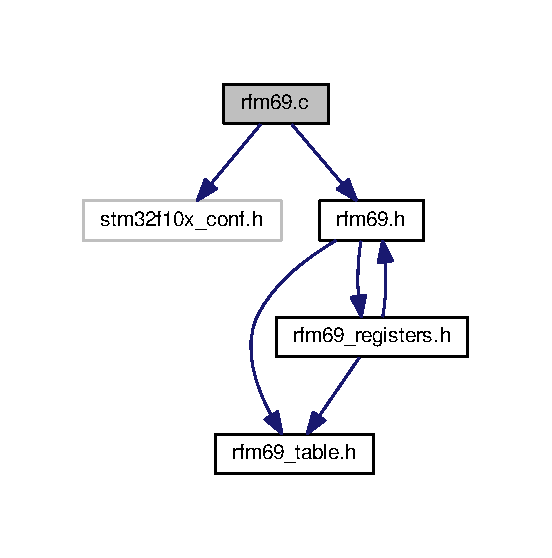
\includegraphics[width=265pt]{rfm69_8c__incl}
\end{center}
\end{figure}
\subsection*{Функции}
\begin{DoxyCompactItemize}
\item 
void \hyperlink{rfm69_8c_ab5a1d9e9c8ef50e0cb9ddb5745a20a14}{E\+X\+T\+I2\+\_\+\+I\+R\+Q\+Handler} (void)
\item 
void \hyperlink{rfm69_8c_a49cfdd46eb8d0ef3e1987514aa9343dc}{E\+X\+T\+I1\+\_\+\+I\+R\+Q\+Handler} (void)
\item 
void \hyperlink{rfm69_8c_a17e9789a29a87d2df54f12b94dd1a0b6}{E\+X\+T\+I0\+\_\+\+I\+R\+Q\+Handler} (void)
\item 
void \hyperlink{rfm69_8c_a38ad4725462bdc5e86c4ead4f04b9fc2}{T\+I\+M2\+\_\+\+I\+R\+Q\+Handler} (void)
\item 
void \hyperlink{rfm69_8c_a14af22393b087d109032f1cf718def90}{rfm69\+\_\+write} (uint8\+\_\+t address, uint8\+\_\+t data)
\item 
uint8\+\_\+t \hyperlink{rfm69_8c_ad2ff4e053c9b555d2192ba3f9af9f5f9}{rfm69\+\_\+read} (uint8\+\_\+t address)
\item 
void \hyperlink{rfm69_8c_af8adfd3a25fb7fd945fe54b25584f391}{rfm69\+\_\+write\+\_\+burst} (uint8\+\_\+t address, uint8\+\_\+t $\ast$data, uint8\+\_\+t ndata)
\item 
void \hyperlink{rfm69_8c_aaf29915020979cbcb1543723e0d1ad09}{rfm69\+\_\+read\+\_\+burst} (uint8\+\_\+t address, uint8\+\_\+t $\ast$data, uint8\+\_\+t ndata)
\item 
void \hyperlink{rfm69_8c_afc18010357577c61751d565f276ec047}{rfm69\+\_\+mcu\+\_\+init} (void)
\item 
int \hyperlink{rfm69_8c_afc9264ee91effa67d4c368944cd2f8a3}{rfm69\+\_\+init} (void)
\item 
int \hyperlink{rfm69_8c_a3141c4360d11844a68888053a7173c2a}{rfm69\+\_\+transmit\+\_\+start} (uint8\+\_\+t packet\+\_\+size\+\_\+loc, uint8\+\_\+t address)
\item 
void \hyperlink{rfm69_8c_a3c042a6544571244615b711a6e7550c7}{rfm69\+\_\+receive\+\_\+start} (void)
\item 
int \hyperlink{rfm69_8c_ac20aaa7a3c508b5086719841909aa059}{rfm69\+\_\+receive\+\_\+small\+\_\+packet} (void)
\item 
void \hyperlink{rfm69_8c_a91f032713bffeee705aeff45e4e8ecbc}{rfm69\+\_\+sleep} (void)
\item 
void \hyperlink{rfm69_8c_a76b7b034cdcbc1d12611ad48a3cfe623}{rfm69\+\_\+stby} (void)
\item 
void \hyperlink{rfm69_8c_a676f160363c34f0bf2638dded13638d7}{rfm69\+\_\+clear\+\_\+fifo} (void)
\end{DoxyCompactItemize}
\subsection*{Переменные}
\begin{DoxyCompactItemize}
\item 
uint8\+\_\+t \hyperlink{rfm69_8c_a0faa461f58d383df212724c389b98a49}{packet\+\_\+buffer} \mbox{[}64\mbox{]}
\item 
uint8\+\_\+t \hyperlink{rfm69_8c_a7f29a961561c7582c38f9a09d859f0a3}{rfm69\+\_\+condition}
\item 
uint8\+\_\+t \hyperlink{rfm69_8c_aee3ef59ff651fe7e6a9c273affdd5d5a}{packet\+\_\+size}
\item 
uint8\+\_\+t \hyperlink{rfm69_8c_a73cc4d50c6a22bbf6aa7481ebd4f8e91}{internal\+\_\+packet\+\_\+buffer} \mbox{[}64\mbox{]}
\item 
uint8\+\_\+t \hyperlink{rfm69_8c_a6c93468e672fcac11316905595027087}{internal\+\_\+pack\+\_\+size}
\end{DoxyCompactItemize}


\subsection{Функции}
\hypertarget{rfm69_8c_a17e9789a29a87d2df54f12b94dd1a0b6}{\index{rfm69.\+c@{rfm69.\+c}!E\+X\+T\+I0\+\_\+\+I\+R\+Q\+Handler@{E\+X\+T\+I0\+\_\+\+I\+R\+Q\+Handler}}
\index{E\+X\+T\+I0\+\_\+\+I\+R\+Q\+Handler@{E\+X\+T\+I0\+\_\+\+I\+R\+Q\+Handler}!rfm69.\+c@{rfm69.\+c}}
\subsubsection[{E\+X\+T\+I0\+\_\+\+I\+R\+Q\+Handler}]{\setlength{\rightskip}{0pt plus 5cm}void E\+X\+T\+I0\+\_\+\+I\+R\+Q\+Handler (
\begin{DoxyParamCaption}
\item[{void}]{}
\end{DoxyParamCaption}
)}}\label{rfm69_8c_a17e9789a29a87d2df54f12b94dd1a0b6}
\hypertarget{rfm69_8c_a49cfdd46eb8d0ef3e1987514aa9343dc}{\index{rfm69.\+c@{rfm69.\+c}!E\+X\+T\+I1\+\_\+\+I\+R\+Q\+Handler@{E\+X\+T\+I1\+\_\+\+I\+R\+Q\+Handler}}
\index{E\+X\+T\+I1\+\_\+\+I\+R\+Q\+Handler@{E\+X\+T\+I1\+\_\+\+I\+R\+Q\+Handler}!rfm69.\+c@{rfm69.\+c}}
\subsubsection[{E\+X\+T\+I1\+\_\+\+I\+R\+Q\+Handler}]{\setlength{\rightskip}{0pt plus 5cm}void E\+X\+T\+I1\+\_\+\+I\+R\+Q\+Handler (
\begin{DoxyParamCaption}
\item[{void}]{}
\end{DoxyParamCaption}
)}}\label{rfm69_8c_a49cfdd46eb8d0ef3e1987514aa9343dc}
\hypertarget{rfm69_8c_ab5a1d9e9c8ef50e0cb9ddb5745a20a14}{\index{rfm69.\+c@{rfm69.\+c}!E\+X\+T\+I2\+\_\+\+I\+R\+Q\+Handler@{E\+X\+T\+I2\+\_\+\+I\+R\+Q\+Handler}}
\index{E\+X\+T\+I2\+\_\+\+I\+R\+Q\+Handler@{E\+X\+T\+I2\+\_\+\+I\+R\+Q\+Handler}!rfm69.\+c@{rfm69.\+c}}
\subsubsection[{E\+X\+T\+I2\+\_\+\+I\+R\+Q\+Handler}]{\setlength{\rightskip}{0pt plus 5cm}void E\+X\+T\+I2\+\_\+\+I\+R\+Q\+Handler (
\begin{DoxyParamCaption}
\item[{void}]{}
\end{DoxyParamCaption}
)}}\label{rfm69_8c_ab5a1d9e9c8ef50e0cb9ddb5745a20a14}
\hypertarget{rfm69_8c_a676f160363c34f0bf2638dded13638d7}{\index{rfm69.\+c@{rfm69.\+c}!rfm69\+\_\+clear\+\_\+fifo@{rfm69\+\_\+clear\+\_\+fifo}}
\index{rfm69\+\_\+clear\+\_\+fifo@{rfm69\+\_\+clear\+\_\+fifo}!rfm69.\+c@{rfm69.\+c}}
\subsubsection[{rfm69\+\_\+clear\+\_\+fifo}]{\setlength{\rightskip}{0pt plus 5cm}void rfm69\+\_\+clear\+\_\+fifo (
\begin{DoxyParamCaption}
\item[{void}]{}
\end{DoxyParamCaption}
)}}\label{rfm69_8c_a676f160363c34f0bf2638dded13638d7}
\hypertarget{rfm69_8c_afc9264ee91effa67d4c368944cd2f8a3}{\index{rfm69.\+c@{rfm69.\+c}!rfm69\+\_\+init@{rfm69\+\_\+init}}
\index{rfm69\+\_\+init@{rfm69\+\_\+init}!rfm69.\+c@{rfm69.\+c}}
\subsubsection[{rfm69\+\_\+init}]{\setlength{\rightskip}{0pt plus 5cm}int rfm69\+\_\+init (
\begin{DoxyParamCaption}
\item[{void}]{}
\end{DoxyParamCaption}
)}}\label{rfm69_8c_afc9264ee91effa67d4c368944cd2f8a3}
\hypertarget{rfm69_8c_afc18010357577c61751d565f276ec047}{\index{rfm69.\+c@{rfm69.\+c}!rfm69\+\_\+mcu\+\_\+init@{rfm69\+\_\+mcu\+\_\+init}}
\index{rfm69\+\_\+mcu\+\_\+init@{rfm69\+\_\+mcu\+\_\+init}!rfm69.\+c@{rfm69.\+c}}
\subsubsection[{rfm69\+\_\+mcu\+\_\+init}]{\setlength{\rightskip}{0pt plus 5cm}void rfm69\+\_\+mcu\+\_\+init (
\begin{DoxyParamCaption}
\item[{void}]{}
\end{DoxyParamCaption}
)}}\label{rfm69_8c_afc18010357577c61751d565f276ec047}
\hypertarget{rfm69_8c_ad2ff4e053c9b555d2192ba3f9af9f5f9}{\index{rfm69.\+c@{rfm69.\+c}!rfm69\+\_\+read@{rfm69\+\_\+read}}
\index{rfm69\+\_\+read@{rfm69\+\_\+read}!rfm69.\+c@{rfm69.\+c}}
\subsubsection[{rfm69\+\_\+read}]{\setlength{\rightskip}{0pt plus 5cm}uint8\+\_\+t rfm69\+\_\+read (
\begin{DoxyParamCaption}
\item[{uint8\+\_\+t}]{address}
\end{DoxyParamCaption}
)}}\label{rfm69_8c_ad2ff4e053c9b555d2192ba3f9af9f5f9}
\hypertarget{rfm69_8c_aaf29915020979cbcb1543723e0d1ad09}{\index{rfm69.\+c@{rfm69.\+c}!rfm69\+\_\+read\+\_\+burst@{rfm69\+\_\+read\+\_\+burst}}
\index{rfm69\+\_\+read\+\_\+burst@{rfm69\+\_\+read\+\_\+burst}!rfm69.\+c@{rfm69.\+c}}
\subsubsection[{rfm69\+\_\+read\+\_\+burst}]{\setlength{\rightskip}{0pt plus 5cm}void rfm69\+\_\+read\+\_\+burst (
\begin{DoxyParamCaption}
\item[{uint8\+\_\+t}]{address, }
\item[{uint8\+\_\+t $\ast$}]{data, }
\item[{uint8\+\_\+t}]{ndata}
\end{DoxyParamCaption}
)}}\label{rfm69_8c_aaf29915020979cbcb1543723e0d1ad09}
\hypertarget{rfm69_8c_ac20aaa7a3c508b5086719841909aa059}{\index{rfm69.\+c@{rfm69.\+c}!rfm69\+\_\+receive\+\_\+small\+\_\+packet@{rfm69\+\_\+receive\+\_\+small\+\_\+packet}}
\index{rfm69\+\_\+receive\+\_\+small\+\_\+packet@{rfm69\+\_\+receive\+\_\+small\+\_\+packet}!rfm69.\+c@{rfm69.\+c}}
\subsubsection[{rfm69\+\_\+receive\+\_\+small\+\_\+packet}]{\setlength{\rightskip}{0pt plus 5cm}int rfm69\+\_\+receive\+\_\+small\+\_\+packet (
\begin{DoxyParamCaption}
\item[{void}]{}
\end{DoxyParamCaption}
)}}\label{rfm69_8c_ac20aaa7a3c508b5086719841909aa059}
\hypertarget{rfm69_8c_a3c042a6544571244615b711a6e7550c7}{\index{rfm69.\+c@{rfm69.\+c}!rfm69\+\_\+receive\+\_\+start@{rfm69\+\_\+receive\+\_\+start}}
\index{rfm69\+\_\+receive\+\_\+start@{rfm69\+\_\+receive\+\_\+start}!rfm69.\+c@{rfm69.\+c}}
\subsubsection[{rfm69\+\_\+receive\+\_\+start}]{\setlength{\rightskip}{0pt plus 5cm}void rfm69\+\_\+receive\+\_\+start (
\begin{DoxyParamCaption}
\item[{void}]{}
\end{DoxyParamCaption}
)}}\label{rfm69_8c_a3c042a6544571244615b711a6e7550c7}
\hypertarget{rfm69_8c_a91f032713bffeee705aeff45e4e8ecbc}{\index{rfm69.\+c@{rfm69.\+c}!rfm69\+\_\+sleep@{rfm69\+\_\+sleep}}
\index{rfm69\+\_\+sleep@{rfm69\+\_\+sleep}!rfm69.\+c@{rfm69.\+c}}
\subsubsection[{rfm69\+\_\+sleep}]{\setlength{\rightskip}{0pt plus 5cm}void rfm69\+\_\+sleep (
\begin{DoxyParamCaption}
\item[{void}]{}
\end{DoxyParamCaption}
)}}\label{rfm69_8c_a91f032713bffeee705aeff45e4e8ecbc}
\hypertarget{rfm69_8c_a76b7b034cdcbc1d12611ad48a3cfe623}{\index{rfm69.\+c@{rfm69.\+c}!rfm69\+\_\+stby@{rfm69\+\_\+stby}}
\index{rfm69\+\_\+stby@{rfm69\+\_\+stby}!rfm69.\+c@{rfm69.\+c}}
\subsubsection[{rfm69\+\_\+stby}]{\setlength{\rightskip}{0pt plus 5cm}void rfm69\+\_\+stby (
\begin{DoxyParamCaption}
\item[{void}]{}
\end{DoxyParamCaption}
)}}\label{rfm69_8c_a76b7b034cdcbc1d12611ad48a3cfe623}
\hypertarget{rfm69_8c_a3141c4360d11844a68888053a7173c2a}{\index{rfm69.\+c@{rfm69.\+c}!rfm69\+\_\+transmit\+\_\+start@{rfm69\+\_\+transmit\+\_\+start}}
\index{rfm69\+\_\+transmit\+\_\+start@{rfm69\+\_\+transmit\+\_\+start}!rfm69.\+c@{rfm69.\+c}}
\subsubsection[{rfm69\+\_\+transmit\+\_\+start}]{\setlength{\rightskip}{0pt plus 5cm}int rfm69\+\_\+transmit\+\_\+start (
\begin{DoxyParamCaption}
\item[{uint8\+\_\+t}]{packet\+\_\+size\+\_\+loc, }
\item[{uint8\+\_\+t}]{address}
\end{DoxyParamCaption}
)}}\label{rfm69_8c_a3141c4360d11844a68888053a7173c2a}
\hypertarget{rfm69_8c_a14af22393b087d109032f1cf718def90}{\index{rfm69.\+c@{rfm69.\+c}!rfm69\+\_\+write@{rfm69\+\_\+write}}
\index{rfm69\+\_\+write@{rfm69\+\_\+write}!rfm69.\+c@{rfm69.\+c}}
\subsubsection[{rfm69\+\_\+write}]{\setlength{\rightskip}{0pt plus 5cm}void rfm69\+\_\+write (
\begin{DoxyParamCaption}
\item[{uint8\+\_\+t}]{address, }
\item[{uint8\+\_\+t}]{data}
\end{DoxyParamCaption}
)}}\label{rfm69_8c_a14af22393b087d109032f1cf718def90}
\hypertarget{rfm69_8c_af8adfd3a25fb7fd945fe54b25584f391}{\index{rfm69.\+c@{rfm69.\+c}!rfm69\+\_\+write\+\_\+burst@{rfm69\+\_\+write\+\_\+burst}}
\index{rfm69\+\_\+write\+\_\+burst@{rfm69\+\_\+write\+\_\+burst}!rfm69.\+c@{rfm69.\+c}}
\subsubsection[{rfm69\+\_\+write\+\_\+burst}]{\setlength{\rightskip}{0pt plus 5cm}void rfm69\+\_\+write\+\_\+burst (
\begin{DoxyParamCaption}
\item[{uint8\+\_\+t}]{address, }
\item[{uint8\+\_\+t $\ast$}]{data, }
\item[{uint8\+\_\+t}]{ndata}
\end{DoxyParamCaption}
)}}\label{rfm69_8c_af8adfd3a25fb7fd945fe54b25584f391}
\hypertarget{rfm69_8c_a38ad4725462bdc5e86c4ead4f04b9fc2}{\index{rfm69.\+c@{rfm69.\+c}!T\+I\+M2\+\_\+\+I\+R\+Q\+Handler@{T\+I\+M2\+\_\+\+I\+R\+Q\+Handler}}
\index{T\+I\+M2\+\_\+\+I\+R\+Q\+Handler@{T\+I\+M2\+\_\+\+I\+R\+Q\+Handler}!rfm69.\+c@{rfm69.\+c}}
\subsubsection[{T\+I\+M2\+\_\+\+I\+R\+Q\+Handler}]{\setlength{\rightskip}{0pt plus 5cm}void T\+I\+M2\+\_\+\+I\+R\+Q\+Handler (
\begin{DoxyParamCaption}
\item[{void}]{}
\end{DoxyParamCaption}
)}}\label{rfm69_8c_a38ad4725462bdc5e86c4ead4f04b9fc2}


\subsection{Переменные}
\hypertarget{rfm69_8c_a6c93468e672fcac11316905595027087}{\index{rfm69.\+c@{rfm69.\+c}!internal\+\_\+pack\+\_\+size@{internal\+\_\+pack\+\_\+size}}
\index{internal\+\_\+pack\+\_\+size@{internal\+\_\+pack\+\_\+size}!rfm69.\+c@{rfm69.\+c}}
\subsubsection[{internal\+\_\+pack\+\_\+size}]{\setlength{\rightskip}{0pt plus 5cm}uint8\+\_\+t internal\+\_\+pack\+\_\+size}}\label{rfm69_8c_a6c93468e672fcac11316905595027087}
\hypertarget{rfm69_8c_a73cc4d50c6a22bbf6aa7481ebd4f8e91}{\index{rfm69.\+c@{rfm69.\+c}!internal\+\_\+packet\+\_\+buffer@{internal\+\_\+packet\+\_\+buffer}}
\index{internal\+\_\+packet\+\_\+buffer@{internal\+\_\+packet\+\_\+buffer}!rfm69.\+c@{rfm69.\+c}}
\subsubsection[{internal\+\_\+packet\+\_\+buffer}]{\setlength{\rightskip}{0pt plus 5cm}uint8\+\_\+t internal\+\_\+packet\+\_\+buffer\mbox{[}64\mbox{]}}}\label{rfm69_8c_a73cc4d50c6a22bbf6aa7481ebd4f8e91}
\hypertarget{rfm69_8c_a0faa461f58d383df212724c389b98a49}{\index{rfm69.\+c@{rfm69.\+c}!packet\+\_\+buffer@{packet\+\_\+buffer}}
\index{packet\+\_\+buffer@{packet\+\_\+buffer}!rfm69.\+c@{rfm69.\+c}}
\subsubsection[{packet\+\_\+buffer}]{\setlength{\rightskip}{0pt plus 5cm}uint8\+\_\+t packet\+\_\+buffer\mbox{[}64\mbox{]}}}\label{rfm69_8c_a0faa461f58d383df212724c389b98a49}
\hypertarget{rfm69_8c_aee3ef59ff651fe7e6a9c273affdd5d5a}{\index{rfm69.\+c@{rfm69.\+c}!packet\+\_\+size@{packet\+\_\+size}}
\index{packet\+\_\+size@{packet\+\_\+size}!rfm69.\+c@{rfm69.\+c}}
\subsubsection[{packet\+\_\+size}]{\setlength{\rightskip}{0pt plus 5cm}uint8\+\_\+t packet\+\_\+size}}\label{rfm69_8c_aee3ef59ff651fe7e6a9c273affdd5d5a}
\hypertarget{rfm69_8c_a7f29a961561c7582c38f9a09d859f0a3}{\index{rfm69.\+c@{rfm69.\+c}!rfm69\+\_\+condition@{rfm69\+\_\+condition}}
\index{rfm69\+\_\+condition@{rfm69\+\_\+condition}!rfm69.\+c@{rfm69.\+c}}
\subsubsection[{rfm69\+\_\+condition}]{\setlength{\rightskip}{0pt plus 5cm}uint8\+\_\+t rfm69\+\_\+condition}}\label{rfm69_8c_a7f29a961561c7582c38f9a09d859f0a3}

\hypertarget{rfm69_8h}{\section{Файл rfm69.\+h}
\label{rfm69_8h}\index{rfm69.\+h@{rfm69.\+h}}
}
{\ttfamily \#include \char`\"{}rfm69\+\_\+table.\+h\char`\"{}}\\*
{\ttfamily \#include \char`\"{}rfm69\+\_\+registers.\+h\char`\"{}}\\*
Граф включаемых заголовочных файлов для rfm69.\+h\+:
\nopagebreak
\begin{figure}[H]
\begin{center}
\leavevmode
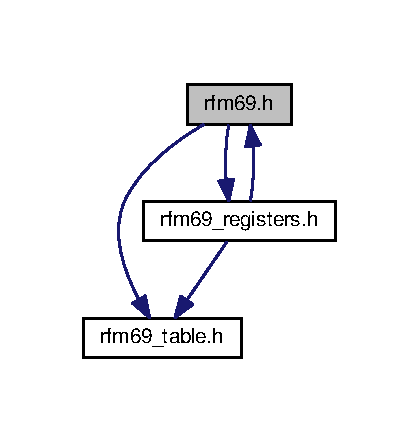
\includegraphics[width=201pt]{rfm69_8h__incl}
\end{center}
\end{figure}
Граф файлов, в которые включается этот файл\+:
\nopagebreak
\begin{figure}[H]
\begin{center}
\leavevmode
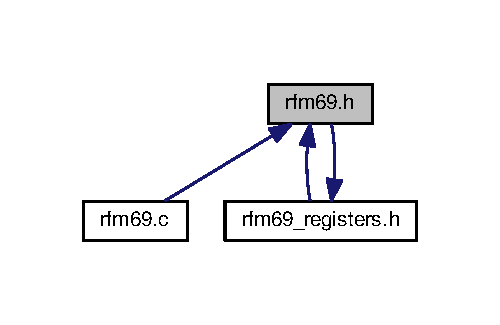
\includegraphics[width=240pt]{rfm69_8h__dep__incl}
\end{center}
\end{figure}
\subsection*{Макросы}
\begin{DoxyCompactItemize}
\item 
\#define \hyperlink{rfm69_8h_a229f2a64968a508915558a93bca313ba}{O\+O\+K}~0x08
\item 
\#define \hyperlink{rfm69_8h_aac78d98bed794339d6bb0ccdb7490776}{F\+S\+K}~0x00
\item 
\#define \hyperlink{rfm69_8h_a17468d10f0c67a4ee7b38aab09d9e096}{B\+I\+T\+R\+A\+T\+E}~9600
\item 
\#define \hyperlink{rfm69_8h_a8fbc13dcb6359fcc5168550fbdc4da41}{C\+A\+R\+R\+I\+E\+R\+\_\+\+F\+R\+E\+Q}~868250000
\item 
\#define \hyperlink{rfm69_8h_a23ecfe0a45f0d87427cf40cd95789f27}{O\+U\+T\+P\+U\+T\+\_\+\+P\+O\+W\+E\+R}~13
\item 
\#define \hyperlink{rfm69_8h_a4a4e7a01439b700bd3a6becd6dd122e0}{R\+X\+\_\+\+B\+W}~65
\item 
\#define \hyperlink{rfm69_8h_aa8796d662eb191d6f49e303b9be80e50}{R\+X\+\_\+\+B\+W\+\_\+\+A\+F\+C}~130
\item 
\#define \hyperlink{rfm69_8h_aa1aa4d62860693257a8a3e23774063f7}{O\+C\+P\+\_\+\+C\+U\+R\+R\+E\+N\+T}~95
\item 
\#define \hyperlink{rfm69_8h_aba3e95cbe8265fef1fe26fbad6c425e8}{M\+O\+D\+U\+L\+\_\+\+T\+Y\+P\+E}~\hyperlink{rfm69_8h_aac78d98bed794339d6bb0ccdb7490776}{F\+S\+K}
\begin{DoxyCompactList}\small\item\em modulation \end{DoxyCompactList}\item 
\#define \hyperlink{rfm69_8h_ab3a2e48ea0f22367d9d3a8ba0ba9a273}{D\+E\+V\+I\+A\+T\+I\+O\+N}~20000
\begin{DoxyCompactList}\small\item\em F\+S\+K parametres. \end{DoxyCompactList}\item 
\#define \hyperlink{rfm69_8h_a661d641b8772cd476fc8c565e5811c65}{R\+I\+S\+E\+\_\+\+F\+A\+L\+L\+\_\+\+T\+I\+M\+E\+\_\+\+F\+S\+K}~50
\item 
\#define \hyperlink{rfm69_8h_ad52736561cde4abc627fc5c4aefbbdb1}{O\+O\+K\+\_\+\+P\+E\+A\+K\+\_\+\+T\+H\+R\+E\+S\+\_\+\+S\+T\+E\+P}~1
\begin{DoxyCompactList}\small\item\em O\+O\+K parametres. \end{DoxyCompactList}\item 
\#define \hyperlink{rfm69_8h_af123b4ef96eb56f98e73951ab76ce314}{O\+O\+K\+\_\+\+P\+E\+A\+K\+\_\+\+T\+H\+R\+E\+S\+H\+\_\+\+D\+E\+C}~1
\item 
\#define \hyperlink{rfm69_8h_a8a06254eb0d3161503e046fcc11dca41}{O\+O\+K\+F\+I\+X\+E\+D\+T\+H\+R\+E\+S\+H}~6
\item 
\#define \hyperlink{rfm69_8h_a8aac8c5098aaf915463fb31715efa09f}{P\+R\+E\+A\+M\+B\+L\+E}~4
\begin{DoxyCompactList}\small\item\em Packet handler configuration. \end{DoxyCompactList}\item 
\#define \hyperlink{rfm69_8h_a1d00740963c7c134022150ed22a0b4d6}{S\+Y\+N\+C\+\_\+\+W\+O\+R\+D\+\_\+\+S\+I\+Z\+E}~4
\item 
\#define \hyperlink{rfm69_8h_a3e9af6b370e370158949ba1f4d064a38}{S\+Y\+N\+C\+\_\+\+W\+O\+R\+D}~0x753be1ca753be1ca
\item 
\#define \hyperlink{rfm69_8h_ab5ef4e3b214d51b79955ceae88e5c4d6}{S\+Y\+N\+C\+T\+O\+L}~2
\item 
\#define \hyperlink{rfm69_8h_a4bc8a54deffcad2b8b0818b86247312a}{R\+X\+\_\+\+A\+D\+D\+R\+E\+S\+S}~0x05
\item 
\#define \hyperlink{rfm69_8h_a294b587d460b14170d2ce3f4da9083ce}{B\+R\+O\+A\+D\+C\+A\+S\+T\+\_\+\+A\+D\+D\+R\+E\+S\+S}~0xff
\item 
\#define \hyperlink{rfm69_8h_aba9ab8b974eb6b97f9af00011e846fca}{A\+U\+T\+O\+\_\+\+R\+E\+S\+T\+A\+R\+T\+\_\+\+R\+X\+\_\+\+D\+E\+L\+A\+Y}~1
\item 
\#define \hyperlink{rfm69_8h_a8c6750b0738c6a321a0253280aea73cd}{R\+S\+S\+I\+\_\+\+T\+H\+R\+E\+S\+H}~88
\item 
\#define \hyperlink{rfm69_8h_a7d44477546ebc96920125d612e718b10}{F\+I\+F\+O\+\_\+\+T\+H\+R\+E\+S\+H\+O\+L\+D}~32
\item 
\#define \hyperlink{rfm69_8h_a53532033984f6c3768b7f0198559bf2e}{C\+U\+T\+\_\+\+O\+F\+F\+\_\+\+F\+R\+E\+Q}~4
\item 
\#define \hyperlink{rfm69_8h_a852de8dab119942f450faa8722897b5b}{C\+U\+T\+\_\+\+O\+F\+F\+\_\+\+F\+R\+E\+Q\+\_\+\+A\+F\+C}~4
\item 
\#define \hyperlink{rfm69_8h_a108423b4512abbd8ed01ddfe33955fd4}{F\+X\+O\+S\+C}~32000000
\item 
\#define \hyperlink{rfm69_8h_aef5e22694322d48a9607f13bb9a4c6f4}{F\+S\+T\+E\+P}~61
\item 
\#define \hyperlink{rfm69_8h_a598a3330b3c21701223ee0ca14316eca}{P\+I}~3.\+14159265359
\item 
\#define \hyperlink{rfm69_8h_afd27d3134ce6a92819d177152bc875b7}{R\+F\+M69\+\_\+\+B\+U\+F\+F\+E\+R\+\_\+\+S\+I\+Z\+E}~66
\item 
\#define \hyperlink{rfm69_8h_aa481f70837b530fa4f47a97a39e99315}{R\+E\+G\+O\+P\+M\+O\+D\+E\+\_\+\+D\+E\+F}~( 0$<$$<$\hyperlink{rfm69__registers_8h_ad34e500db60585f5c256b04bd898ebba}{S\+E\+Q\+U\+E\+N\+C\+E\+R\+O\+F\+F} $\vert$ 0$<$$<$\hyperlink{rfm69__registers_8h_ac873ed4655b1b8770ef2994e5c02c5d7}{L\+I\+S\+T\+E\+N\+O\+N} $\vert$ \hyperlink{rfm69__registers_8h_a6097218fc13c9936e96507d6fd9fafe0}{S\+L\+E\+E\+P\+\_\+\+M\+O\+D\+E} )
\item 
\#define \hyperlink{rfm69_8h_a24e619d07fe3e5facc0f32f6d8b759d4}{R\+E\+G\+D\+A\+T\+A\+M\+O\+D\+U\+L\+\_\+\+D\+E\+F}~( \hyperlink{rfm69__registers_8h_a366d2e1ca64909f289bde16361b6fd07}{P\+A\+C\+K\+E\+T\+\_\+\+M\+O\+D\+E} $\vert$ \hyperlink{rfm69_8h_aba3e95cbe8265fef1fe26fbad6c425e8}{M\+O\+D\+U\+L\+\_\+\+T\+Y\+P\+E} $\vert$ \hyperlink{rfm69__registers_8h_a4a70bc27906df4705fba032b0bcec59b}{G\+A\+U\+S\+S\+\_\+\+B\+T10} )
\item 
\#define \hyperlink{rfm69_8h_ace2a7039f469e7855b4308a3ed6f4a4a}{R\+E\+G\+F\+D\+E\+V\+M\+S\+B\+\_\+\+D\+E\+F}~( (\hyperlink{rfm69__registers_8h_a77666bfe5e6e90bb35003fa957f9ec6f}{F\+D\+E\+V\+\_\+\+C\+A\+L\+C}(\hyperlink{rfm69_8h_ab3a2e48ea0f22367d9d3a8ba0ba9a273}{D\+E\+V\+I\+A\+T\+I\+O\+N}) \& 0xff00) $>$$>$ 8 )
\item 
\#define \hyperlink{rfm69_8h_afdd474d90ee06120e80cd844389c8d73}{R\+E\+G\+F\+D\+E\+V\+L\+S\+B\+\_\+\+D\+E\+F}~(  \hyperlink{rfm69__registers_8h_a77666bfe5e6e90bb35003fa957f9ec6f}{F\+D\+E\+V\+\_\+\+C\+A\+L\+C}(\hyperlink{rfm69_8h_ab3a2e48ea0f22367d9d3a8ba0ba9a273}{D\+E\+V\+I\+A\+T\+I\+O\+N}) \& 0x00ff )
\item 
\#define \hyperlink{rfm69_8h_a0d47227ea1b41e85a8ed141f355ad32e}{R\+E\+G\+B\+I\+T\+R\+A\+T\+E\+M\+S\+B\+\_\+\+D\+E\+F}~( (\hyperlink{rfm69__registers_8h_ac1ae7970d0dcf267a7a5ca51687d97fe}{B\+I\+T\+R\+A\+T\+E\+\_\+\+C\+A\+L\+C}(\hyperlink{rfm69_8h_a17468d10f0c67a4ee7b38aab09d9e096}{B\+I\+T\+R\+A\+T\+E}) \& 0xff00) $>$$>$ 8 )
\item 
\#define \hyperlink{rfm69_8h_a059f8fd70a7d8cefa34bbf0bc0bbcaef}{R\+E\+G\+B\+I\+T\+R\+A\+T\+E\+L\+S\+B\+\_\+\+D\+E\+F}~(  \hyperlink{rfm69__registers_8h_ac1ae7970d0dcf267a7a5ca51687d97fe}{B\+I\+T\+R\+A\+T\+E\+\_\+\+C\+A\+L\+C}(\hyperlink{rfm69_8h_a17468d10f0c67a4ee7b38aab09d9e096}{B\+I\+T\+R\+A\+T\+E}) \& 0x00ff )
\item 
\#define \hyperlink{rfm69_8h_a1c20d269c21c060a659e69102a6d095c}{R\+E\+G\+F\+R\+F\+M\+S\+B\+\_\+\+D\+E\+F}~( (\hyperlink{rfm69__registers_8h_ae902e7a3545149f07d33ebeea9e3ba11}{F\+R\+F\+\_\+\+C\+A\+L\+C}(\hyperlink{rfm69_8h_a8fbc13dcb6359fcc5168550fbdc4da41}{C\+A\+R\+R\+I\+E\+R\+\_\+\+F\+R\+E\+Q}) \& 0xff0000) $>$$>$ 16 )
\item 
\#define \hyperlink{rfm69_8h_aa1d73304222c089ef07081fe2481ebf7}{R\+E\+G\+F\+R\+F\+M\+I\+D\+\_\+\+D\+E\+F}~( (\hyperlink{rfm69__registers_8h_ae902e7a3545149f07d33ebeea9e3ba11}{F\+R\+F\+\_\+\+C\+A\+L\+C}(\hyperlink{rfm69_8h_a8fbc13dcb6359fcc5168550fbdc4da41}{C\+A\+R\+R\+I\+E\+R\+\_\+\+F\+R\+E\+Q}) \& 0x00ff00) $>$$>$ 8 )
\item 
\#define \hyperlink{rfm69_8h_aad391d879f9a8f94ff1f6b613389eaa9}{R\+E\+G\+F\+R\+F\+L\+S\+B\+\_\+\+D\+E\+F}~(  \hyperlink{rfm69__registers_8h_ae902e7a3545149f07d33ebeea9e3ba11}{F\+R\+F\+\_\+\+C\+A\+L\+C}(\hyperlink{rfm69_8h_a8fbc13dcb6359fcc5168550fbdc4da41}{C\+A\+R\+R\+I\+E\+R\+\_\+\+F\+R\+E\+Q}) \& 0x0000ff )
\item 
\#define \hyperlink{rfm69_8h_a37446f6c54ea6ee20ae9d1490e259ae4}{R\+E\+G\+A\+F\+C\+C\+T\+R\+L\+\_\+\+D\+E\+F}~( 0$<$$<$(\hyperlink{rfm69__registers_8h_ad5d2eba8b4963a97848a746ba9094346}{A\+F\+C\+L\+O\+W\+B\+E\+T\+A\+O\+N}) )
\item 
\#define \hyperlink{rfm69_8h_ac466d41919e6f9a9abb07dee89e5e509}{R\+E\+G\+L\+I\+S\+T\+E\+N1\+\_\+\+D\+E\+F}~( 0x00 )
\item 
\#define \hyperlink{rfm69_8h_a744e206075b979d38857e336efefa838}{R\+E\+G\+L\+I\+S\+T\+E\+N2\+\_\+\+D\+E\+F}~( 0x00 )
\item 
\#define \hyperlink{rfm69_8h_a10ca27af91cffe9a96dc6059cde3af76}{R\+E\+G\+L\+I\+S\+T\+E\+N3\+\_\+\+D\+E\+F}~( 0x00 )
\item 
\#define \hyperlink{rfm69_8h_a4a6fb558c267560bca4250e1c3b7f099}{R\+E\+G\+P\+A\+L\+E\+V\+E\+L\+\_\+\+D\+E\+F}~( 1$<$$<$\hyperlink{rfm69__registers_8h_a1349892a7adac828df5ab3a395e557e0}{P\+A0\+O\+N} $\vert$ 0$<$$<$\hyperlink{rfm69__registers_8h_a0048b53a5557ee80b7792fde9f976ba5}{P\+A1\+O\+N} $\vert$ 0$<$$<$\hyperlink{rfm69__registers_8h_ae5a87eb57ec917fd5b5fe4083875e19a}{P\+A2\+O\+N} $\vert$ (\hyperlink{rfm69__registers_8h_acb5c8c4439d716b93a8d4767ac398e60}{O\+U\+T\+\_\+\+P\+O\+W\+E\+R\+\_\+\+C\+A\+L\+C}(\hyperlink{rfm69_8h_a23ecfe0a45f0d87427cf40cd95789f27}{O\+U\+T\+P\+U\+T\+\_\+\+P\+O\+W\+E\+R})) )
\item 
\#define \hyperlink{rfm69_8h_a6bbce267488fbde0e103bd7895425a48}{R\+E\+G\+P\+A\+R\+A\+M\+P\+\_\+\+D\+E\+F}~( \hyperlink{rfm69__table_8h_ab1c78669a770ddfb58e99c063225f32f}{P\+A\+R\+A\+M\+P} )
\item 
\#define \hyperlink{rfm69_8h_a37f49e9dab08064c9bbbd9adadcc7206}{R\+E\+G\+O\+C\+P\+\_\+\+D\+E\+F}~( 1$<$$<$\hyperlink{rfm69__registers_8h_a241fa810dd7c750734cf4d02893a8aaf}{O\+C\+P\+O\+N}	$\vert$ (\hyperlink{rfm69__registers_8h_aedcc657b574a4c9f7956f94ad2e65d4a}{O\+C\+P\+\_\+\+C\+U\+R\+R\+E\+N\+T\+\_\+\+C\+A\+L\+C}(\hyperlink{rfm69_8h_aa1aa4d62860693257a8a3e23774063f7}{O\+C\+P\+\_\+\+C\+U\+R\+R\+E\+N\+T})) )
\item 
\#define \hyperlink{rfm69_8h_ab155c7ec3074d618035101f097a0d734}{R\+E\+G\+L\+N\+A\+\_\+\+D\+E\+F}~( 1$<$$<$\hyperlink{rfm69__registers_8h_a95610ecbca4757054e9becc0f6da8001}{L\+N\+A\+Z\+I\+N} $\vert$ \hyperlink{rfm69__registers_8h_a49a78405e3eb02eaf9ffc105a608f478}{L\+N\+A\+G\+A\+I\+N\+\_\+\+A\+U\+T\+O} )
\item 
\#define \hyperlink{rfm69_8h_ae21147f19d0a85394abdb4cdf6d6f099}{R\+E\+G\+R\+X\+B\+W\+\_\+\+D\+E\+F}~( D\+C\+C\+F\+R\+E\+Q $\vert$ \hyperlink{rfm69__table_8h_ade419dfc07a685580dd336aa324f17ad}{R\+X\+B\+W} )
\item 
\#define \hyperlink{rfm69_8h_a83bd804449c3b53827fb334ed871c2ef}{R\+E\+G\+A\+F\+C\+B\+W\+\_\+\+D\+E\+F}~( D\+C\+C\+F\+R\+E\+Q\+A\+F\+C $\vert$ R\+X\+B\+W\+A\+F\+C )
\item 
\#define \hyperlink{rfm69_8h_a4b4a58302244d924e5fe1c0fa676b143}{R\+E\+G\+O\+O\+K\+P\+E\+A\+K\+\_\+\+D\+E\+F}~( 0x00 )
\item 
\#define \hyperlink{rfm69_8h_ae85fcceb41012504b3939be585b76646}{R\+E\+G\+O\+O\+K\+A\+V\+G\+\_\+\+D\+E\+F}~( 0x00 )
\item 
\#define \hyperlink{rfm69_8h_a8b5a4d8e8e8842be6c606481af7c691d}{R\+E\+G\+O\+O\+K\+F\+I\+X\+\_\+\+D\+E\+F}~( 0x00 )
\item 
\#define \hyperlink{rfm69_8h_a3549c6f967228085201f21c160e5e24a}{R\+E\+G\+A\+F\+C\+F\+E\+I\+\_\+\+D\+E\+F}~( (1$<$$<$\hyperlink{rfm69__registers_8h_ac3f3f8de47d947af91e9b12e8a461e2c}{A\+F\+C\+A\+U\+T\+O\+C\+L\+E\+A\+R}) $\vert$ (1$<$$<$\hyperlink{rfm69__registers_8h_ab65fcdba5953290d2b432eab78862c90}{A\+F\+C\+A\+U\+T\+O\+O\+N}) )
\item 
\#define \hyperlink{rfm69_8h_a49498083cf536aa97ac7013559e62f80}{R\+E\+G\+D\+I\+O\+M\+A\+P\+P\+I\+N\+G1\+\_\+\+D\+E\+F}~( \hyperlink{rfm69__registers_8h_a4f3496e7ca63e021951eb2710254afa1}{D\+I\+O0\+M\+A\+P0} $\vert$ \hyperlink{rfm69__registers_8h_a45c774244e4f9ecc7b74c3d27c3c9e25}{D\+I\+O1\+M\+A\+P0} $\vert$ \hyperlink{rfm69__registers_8h_a3247a01dec1629f6cb03b84784d84bbe}{D\+I\+O2\+M\+A\+P2} $\vert$ \hyperlink{rfm69__registers_8h_af9f9c18fc5ead63d4aaa535177542834}{D\+I\+O3\+M\+A\+P1} )
\item 
\#define \hyperlink{rfm69_8h_aa0ffae0f96a59ee7baffe72d2103b821}{R\+E\+G\+D\+I\+O\+M\+A\+P\+P\+I\+N\+G2\+\_\+\+D\+E\+F}~( \hyperlink{rfm69__registers_8h_a72f94132418287bf937d1d3bbd4becb4}{D\+I\+O5\+M\+A\+P0} $\vert$ \hyperlink{rfm69__registers_8h_ac9da285bce38f36312291a81815b7f09}{C\+L\+K\+O\+U\+T8\+M} )
\item 
\#define \hyperlink{rfm69_8h_a88592234f9104d00e24fb7cb02ffddb3}{R\+E\+G\+R\+S\+S\+I\+T\+H\+R\+E\+S\+H\+\_\+\+D\+E\+F}~( \hyperlink{rfm69__registers_8h_aab1351f68c4bd1865fae376734674afd}{R\+S\+S\+I\+\_\+\+T\+H\+R\+E\+S\+H\+\_\+\+C\+A\+L\+C}(\hyperlink{rfm69_8h_a8c6750b0738c6a321a0253280aea73cd}{R\+S\+S\+I\+\_\+\+T\+H\+R\+E\+S\+H}) )
\item 
\#define \hyperlink{rfm69_8h_a41db30e231f76a5d2d04fb9464682221}{R\+E\+G\+P\+R\+E\+A\+M\+B\+L\+E\+M\+S\+B\+\_\+\+D\+E\+F}~( (\hyperlink{rfm69_8h_a8aac8c5098aaf915463fb31715efa09f}{P\+R\+E\+A\+M\+B\+L\+E} \& 0xff00) $>$$>$ 8 )
\item 
\#define \hyperlink{rfm69_8h_a36c1e97cbe8818ea8ce402f81c3e426f}{R\+E\+G\+P\+R\+E\+A\+M\+B\+L\+E\+L\+S\+B\+\_\+\+D\+E\+F}~( \hyperlink{rfm69_8h_a8aac8c5098aaf915463fb31715efa09f}{P\+R\+E\+A\+M\+B\+L\+E} \& 0x00ff )
\item 
\#define \hyperlink{rfm69_8h_ad45d749cfbd080b1ade430d184259665}{R\+E\+G\+S\+Y\+N\+C\+C\+O\+N\+F\+I\+G\+\_\+\+D\+E\+F}~( \hyperlink{rfm69__registers_8h_ae106483494497c8026ab22e1ef8fcdf6}{S\+Y\+N\+C\+\_\+\+W\+O\+R\+D\+\_\+\+O\+N} $\vert$ 0$<$$<$\hyperlink{rfm69__registers_8h_ad5136933340ac95954fc304b58fc005c}{F\+I\+F\+O\+F\+I\+L\+L\+C\+O\+N\+D} $\vert$ \hyperlink{rfm69__registers_8h_acd179fc969c2f0e41b6bd5e1aa7906f1}{S\+Y\+N\+C\+S\+I\+Z\+E\+\_\+\+C\+A\+L\+C}(\hyperlink{rfm69_8h_a1d00740963c7c134022150ed22a0b4d6}{S\+Y\+N\+C\+\_\+\+W\+O\+R\+D\+\_\+\+S\+I\+Z\+E}) $\vert$ (\hyperlink{rfm69_8h_ab5ef4e3b214d51b79955ceae88e5c4d6}{S\+Y\+N\+C\+T\+O\+L}\&0x07) )
\item 
\#define \hyperlink{rfm69_8h_abb8b6a0817157e19c1459b528609bef6}{R\+E\+G\+S\+Y\+N\+C\+V\+A\+L\+U\+E1\+\_\+\+D\+E\+F}~(  \hyperlink{rfm69_8h_a3e9af6b370e370158949ba1f4d064a38}{S\+Y\+N\+C\+\_\+\+W\+O\+R\+D} \& 0x00000000000000ff )
\item 
\#define \hyperlink{rfm69_8h_a5938c1eed62833fd33833926b605daad}{R\+E\+G\+S\+Y\+N\+C\+V\+A\+L\+U\+E2\+\_\+\+D\+E\+F}~( (\hyperlink{rfm69_8h_a3e9af6b370e370158949ba1f4d064a38}{S\+Y\+N\+C\+\_\+\+W\+O\+R\+D} \& 0x000000000000ff00) $>$$>$ 8 )
\item 
\#define \hyperlink{rfm69_8h_a3e4146486356d6d599ac7ab25367edf2}{R\+E\+G\+S\+Y\+N\+C\+V\+A\+L\+U\+E3\+\_\+\+D\+E\+F}~( (\hyperlink{rfm69_8h_a3e9af6b370e370158949ba1f4d064a38}{S\+Y\+N\+C\+\_\+\+W\+O\+R\+D} \& 0x0000000000ff0000) $>$$>$ 16 )
\item 
\#define \hyperlink{rfm69_8h_a2cc875d0068b61df3a073cda2e3f92c7}{R\+E\+G\+S\+Y\+N\+C\+V\+A\+L\+U\+E4\+\_\+\+D\+E\+F}~( (\hyperlink{rfm69_8h_a3e9af6b370e370158949ba1f4d064a38}{S\+Y\+N\+C\+\_\+\+W\+O\+R\+D} \& 0x00000000ff000000) $>$$>$ 24 )
\item 
\#define \hyperlink{rfm69_8h_ae75d99c6b7e350e913fadad0ba291f8b}{R\+E\+G\+S\+Y\+N\+C\+V\+A\+L\+U\+E5\+\_\+\+D\+E\+F}~( (\hyperlink{rfm69_8h_a3e9af6b370e370158949ba1f4d064a38}{S\+Y\+N\+C\+\_\+\+W\+O\+R\+D} \& 0x000000ff00000000) $>$$>$ 32 )
\item 
\#define \hyperlink{rfm69_8h_a621156521341eaef210ff6b989b558e8}{R\+E\+G\+S\+Y\+N\+C\+V\+A\+L\+U\+E6\+\_\+\+D\+E\+F}~( (\hyperlink{rfm69_8h_a3e9af6b370e370158949ba1f4d064a38}{S\+Y\+N\+C\+\_\+\+W\+O\+R\+D} \& 0x0000ff0000000000) $>$$>$ 40 )
\item 
\#define \hyperlink{rfm69_8h_a4964b030f4dcb285357b3b2e14f6a846}{R\+E\+G\+S\+Y\+N\+C\+V\+A\+L\+U\+E7\+\_\+\+D\+E\+F}~( (\hyperlink{rfm69_8h_a3e9af6b370e370158949ba1f4d064a38}{S\+Y\+N\+C\+\_\+\+W\+O\+R\+D} \& 0x00ff000000000000) $>$$>$ 48 )
\item 
\#define \hyperlink{rfm69_8h_a0a73edb0344f2832c428d70efc4c93b2}{R\+E\+G\+S\+Y\+N\+C\+V\+A\+L\+U\+E8\+\_\+\+D\+E\+F}~( (\hyperlink{rfm69_8h_a3e9af6b370e370158949ba1f4d064a38}{S\+Y\+N\+C\+\_\+\+W\+O\+R\+D} \& 0xff00000000000000) $>$$>$ 56 )
\item 
\#define \hyperlink{rfm69_8h_a4edc7c51a6b7019f02aaac0153cfe291}{R\+E\+G\+P\+A\+C\+K\+E\+T\+C\+O\+N\+F\+I\+G1\+\_\+\+D\+E\+F}~( 1$<$$<$\hyperlink{rfm69__registers_8h_a5db0212961ff5494d1c9d6efdcf03730}{P\+A\+C\+K\+E\+T\+F\+O\+R\+M\+A\+T} $\vert$ \hyperlink{rfm69__registers_8h_a15df7bdfa2cb6787bd141aefc0f93e12}{E\+N\+C\+O\+D\+I\+N\+G\+\_\+\+O\+F\+F} $\vert$ 1$<$$<$\hyperlink{rfm69__registers_8h_a73c706d20d14f72e4864392b4bad9799}{C\+R\+C\+O\+N} $\vert$ 0$<$$<$\hyperlink{rfm69__registers_8h_ad5bfb4aedaab8eef409e4e7838caa375}{C\+R\+C\+A\+U\+T\+O\+C\+L\+E\+A\+R\+O\+F\+F} $\vert$ \hyperlink{rfm69__registers_8h_ab3f7692a1ea401ba18ca18246ebef425}{N\+O\+D\+E\+\_\+\+B\+R\+O\+A\+D\+C\+A\+S\+T\+\_\+\+A\+D\+D\+R})
\item 
\#define \hyperlink{rfm69_8h_ac435942286d0fbaa4a2348b1d6b03149}{R\+E\+G\+P\+A\+Y\+L\+O\+A\+D\+L\+E\+N\+G\+H\+T\+\_\+\+D\+E\+F}~( 0xff )
\item 
\#define \hyperlink{rfm69_8h_acf240a368a432961a78b49c8929d9cf8}{R\+E\+G\+N\+O\+D\+E\+A\+D\+R\+S\+\_\+\+D\+E\+F}~( \hyperlink{rfm69_8h_a4bc8a54deffcad2b8b0818b86247312a}{R\+X\+\_\+\+A\+D\+D\+R\+E\+S\+S} )
\item 
\#define \hyperlink{rfm69_8h_a32a04d199c1544c555dee9cfe22b493c}{R\+E\+G\+B\+R\+O\+A\+D\+C\+A\+S\+T\+A\+D\+R\+S\+\_\+\+D\+E\+F}~( \hyperlink{rfm69_8h_a294b587d460b14170d2ce3f4da9083ce}{B\+R\+O\+A\+D\+C\+A\+S\+T\+\_\+\+A\+D\+D\+R\+E\+S\+S} )
\item 
\#define \hyperlink{rfm69_8h_adca98589141cfeb6c3e890100a20f4e6}{R\+E\+G\+A\+U\+T\+O\+M\+O\+D\+E\+S\+\_\+\+D\+E\+F}~( 0x00 )
\item 
\#define \hyperlink{rfm69_8h_a80f5b2e2d127d5b33010280ef26bbad3}{R\+E\+G\+F\+I\+F\+O\+T\+H\+R\+E\+S\+\_\+\+D\+E\+F}~( 1$<$$<$\hyperlink{rfm69__registers_8h_a7500b77df8de3795a4eb235ed24c70f3}{T\+X\+S\+T\+A\+R\+T\+C\+O\+N\+D} $\vert$ (\hyperlink{rfm69_8h_a7d44477546ebc96920125d612e718b10}{F\+I\+F\+O\+\_\+\+T\+H\+R\+E\+S\+H\+O\+L\+D}\&0x7f) )
\item 
\#define \hyperlink{rfm69_8h_a8b312d3af71aabaa16ac6bccd20e56c8}{R\+E\+G\+P\+A\+C\+K\+E\+T\+C\+O\+N\+F\+I\+G2\+\_\+\+D\+E\+F}~( \hyperlink{rfm69__table_8h_aa2f9059f987d6088a0b77a2af76e3ab2}{I\+N\+T\+E\+R\+P\+A\+C\+K\+E\+T\+R\+X\+D\+E\+L\+A\+Y} $\vert$ 1$<$$<$\hyperlink{rfm69__registers_8h_a2056d2ccf745e838f1436ce70d8e81ff}{A\+U\+T\+O\+R\+X\+R\+E\+S\+T\+A\+R\+T\+O\+N} $\vert$ 0$<$$<$\hyperlink{rfm69__registers_8h_a329c471460a05db1a3cfb2c357465529}{A\+E\+S\+O\+N} )
\item 
\#define \hyperlink{rfm69_8h_a41b4bd5e1c812d2c0c4fc175f7416804}{R\+E\+G\+A\+E\+S\+K\+E\+Y1\+\_\+\+D\+E\+F}~( 0x00 )
\item 
\#define \hyperlink{rfm69_8h_a81b13a3ea9b82e96d01fb76ede373578}{R\+E\+G\+A\+E\+S\+K\+E\+Y2\+\_\+\+D\+E\+F}~( 0x00 )
\item 
\#define \hyperlink{rfm69_8h_a5f16df0f4a3c405ce57bb25441a34f2f}{R\+E\+G\+A\+E\+S\+K\+E\+Y3\+\_\+\+D\+E\+F}~( 0x00 )
\item 
\#define \hyperlink{rfm69_8h_a743a411748a454195cd543fd3fa2e80f}{R\+E\+G\+A\+E\+S\+K\+E\+Y4\+\_\+\+D\+E\+F}~( 0x00 )
\item 
\#define \hyperlink{rfm69_8h_ad8689cd7abb93ca0f9548aa8e704f81d}{R\+E\+G\+A\+E\+S\+K\+E\+Y5\+\_\+\+D\+E\+F}~( 0x00 )
\item 
\#define \hyperlink{rfm69_8h_ac6bf8865dda1078012bb86e903034f46}{R\+E\+G\+A\+E\+S\+K\+E\+Y6\+\_\+\+D\+E\+F}~( 0x00 )
\item 
\#define \hyperlink{rfm69_8h_afd145bb3bbc38eae1921221e10dca955}{R\+E\+G\+A\+E\+S\+K\+E\+Y7\+\_\+\+D\+E\+F}~( 0x00 )
\item 
\#define \hyperlink{rfm69_8h_a3ef01a4b58d93969d9e780dd1feb81b5}{R\+E\+G\+A\+E\+S\+K\+E\+Y8\+\_\+\+D\+E\+F}~( 0x00 )
\item 
\#define \hyperlink{rfm69_8h_af75dd93e24e4c14c6467cf2be42f8fd4}{R\+E\+G\+A\+E\+S\+K\+E\+Y9\+\_\+\+D\+E\+F}~( 0x00 )
\item 
\#define \hyperlink{rfm69_8h_ac549a0a5b4d2bac59255f57236f2a991}{R\+E\+G\+A\+E\+S\+K\+E\+Y10\+\_\+\+D\+E\+F}~( 0x00 )
\item 
\#define \hyperlink{rfm69_8h_a557d80768e46c07e52b68e79b9245f85}{R\+E\+G\+A\+E\+S\+K\+E\+Y11\+\_\+\+D\+E\+F}~( 0x00 )
\item 
\#define \hyperlink{rfm69_8h_a6ab4399dffd4d837bc1c7aedc8df01ef}{R\+E\+G\+A\+E\+S\+K\+E\+Y12\+\_\+\+D\+E\+F}~( 0x00 )
\item 
\#define \hyperlink{rfm69_8h_a321d435524c9ce359d633b5b00e659f1}{R\+E\+G\+A\+E\+S\+K\+E\+Y13\+\_\+\+D\+E\+F}~( 0x00 )
\item 
\#define \hyperlink{rfm69_8h_a2ebc9cd28d516436e5acaf720533842d}{R\+E\+G\+A\+E\+S\+K\+E\+Y14\+\_\+\+D\+E\+F}~( 0x00 )
\item 
\#define \hyperlink{rfm69_8h_a684147b2e747d9ef12fc7fee45284bc0}{R\+E\+G\+A\+E\+S\+K\+E\+Y15\+\_\+\+D\+E\+F}~( 0x00 )
\item 
\#define \hyperlink{rfm69_8h_a94e15c31c6e1f43c5c48583920f3f039}{R\+E\+G\+A\+E\+S\+K\+E\+Y16\+\_\+\+D\+E\+F}~( 0x00 )
\item 
\#define \hyperlink{rfm69_8h_a9d5d5f54264410cda15c20060e6265cd}{C\+R\+C\+O\+K\+\_\+\+P\+K\+Sent\+\_\+\+Line}~E\+X\+T\+I\+\_\+\+Line2
\item 
\#define \hyperlink{rfm69_8h_a804ae6b1a8127fc52b4f6742cbbb03f2}{Fifo\+Level\+\_\+\+Line}~E\+X\+T\+I\+\_\+\+Line1
\item 
\#define \hyperlink{rfm69_8h_ab9e0536e23e13affa9c84d6f6259172d}{Sync\+Addr\+\_\+\+Line}~E\+X\+T\+I\+\_\+\+Line0
\item 
\#define \hyperlink{rfm69_8h_a8bce2f7b28914b649b55dc779c66838a}{N\+S\+S\+\_\+\+Port}~G\+P\+I\+O\+A
\item 
\#define \hyperlink{rfm69_8h_aedbee85879aa9a3d494f0502ad1f82cd}{N\+S\+S\+\_\+\+Pin}~G\+P\+I\+O\+\_\+\+Pin\+\_\+3
\item 
\#define \hyperlink{rfm69_8h_af402a3554782ca9b66273776a516cdc9}{E\+X\+T\+I\+\_\+\+Port1}~G\+P\+I\+O\+\_\+\+Port\+Source\+G\+P\+I\+O\+B
\item 
\#define \hyperlink{rfm69_8h_afdefc677cae2122279f3aeeb3f6cb3c8}{E\+X\+T\+I\+\_\+\+Port23}~G\+P\+I\+O\+\_\+\+Port\+Source\+G\+P\+I\+O\+A
\item 
\#define \hyperlink{rfm69_8h_a83302997180949ef0538ffaaacf1d832}{E\+X\+T\+I\+\_\+\+Pin1}~G\+P\+I\+O\+\_\+\+Pin\+Source0
\item 
\#define \hyperlink{rfm69_8h_a7021fc9bc0f7bf9e98ba7264b2e5cbff}{E\+X\+T\+I\+\_\+\+Pin2}~G\+P\+I\+O\+\_\+\+Pin\+Source1
\item 
\#define \hyperlink{rfm69_8h_a13e8a49e0edf0710a362ba4efa8f6533}{E\+X\+T\+I\+\_\+\+Pin3}~G\+P\+I\+O\+\_\+\+Pin\+Source2
\item 
\#define \hyperlink{rfm69_8h_add1b7df122f5f0dc96eb8dfd3d0a80ff}{R\+F\+M69\+\_\+\+S\+Y\+N\+C\+A\+D\+D\+R\+\_\+\+P\+E\+R\+I\+O\+D}~\hyperlink{rfm69_8h_a8aac8c5098aaf915463fb31715efa09f}{P\+R\+E\+A\+M\+B\+L\+E} + \hyperlink{rfm69_8h_a1d00740963c7c134022150ed22a0b4d6}{S\+Y\+N\+C\+\_\+\+W\+O\+R\+D\+\_\+\+S\+I\+Z\+E} + 1
\end{DoxyCompactItemize}
\subsection*{Перечисления}
\begin{DoxyCompactItemize}
\item 
enum \{ \\*
\hyperlink{rfm69_8h_a06fc87d81c62e9abb8790b6e5713c55ba100341cd68397fd697b86439b4aca9ed}{R\+F\+M69\+\_\+\+S\+P\+I\+\_\+\+F\+A\+I\+L\+E\+D} = 1, 
\hyperlink{rfm69_8h_a06fc87d81c62e9abb8790b6e5713c55ba0f464bbbdc9e2e6795f713e194521c3d}{R\+F\+M69\+\_\+\+S\+L\+E\+E\+P}, 
\hyperlink{rfm69_8h_a06fc87d81c62e9abb8790b6e5713c55bace14731600372a2f328a5cd727570fbc}{R\+F\+M69\+\_\+\+S\+T\+B\+Y}, 
\hyperlink{rfm69_8h_a06fc87d81c62e9abb8790b6e5713c55ba778608da6788aae63668b8511bba32a1}{R\+F\+M69\+\_\+\+R\+X}, 
\\*
\hyperlink{rfm69_8h_a06fc87d81c62e9abb8790b6e5713c55ba289aded594cf744abe36d6126736a06e}{R\+F\+M69\+\_\+\+T\+X}, 
\hyperlink{rfm69_8h_a06fc87d81c62e9abb8790b6e5713c55badc0a15b8d6e072ff02e1e89e35a73226}{R\+F\+M69\+\_\+\+N\+E\+W\+\_\+\+P\+A\+C\+K}
 \}
\end{DoxyCompactItemize}
\subsection*{Функции}
\begin{DoxyCompactItemize}
\item 
void \hyperlink{rfm69_8h_a14af22393b087d109032f1cf718def90}{rfm69\+\_\+write} (uint8\+\_\+t address, uint8\+\_\+t data)
\item 
uint8\+\_\+t \hyperlink{rfm69_8h_ad2ff4e053c9b555d2192ba3f9af9f5f9}{rfm69\+\_\+read} (uint8\+\_\+t address)
\item 
void \hyperlink{rfm69_8h_af8adfd3a25fb7fd945fe54b25584f391}{rfm69\+\_\+write\+\_\+burst} (uint8\+\_\+t address, uint8\+\_\+t $\ast$data, uint8\+\_\+t ndata)
\item 
void \hyperlink{rfm69_8h_aaf29915020979cbcb1543723e0d1ad09}{rfm69\+\_\+read\+\_\+burst} (uint8\+\_\+t address, uint8\+\_\+t $\ast$data, uint8\+\_\+t ndata)
\item 
void \hyperlink{rfm69_8h_afc18010357577c61751d565f276ec047}{rfm69\+\_\+mcu\+\_\+init} (void)
\item 
int \hyperlink{rfm69_8h_afc9264ee91effa67d4c368944cd2f8a3}{rfm69\+\_\+init} (void)
\item 
int \hyperlink{rfm69_8h_a13883b87b275d312974ef052cdccef86}{rfm69\+\_\+transmit\+\_\+start} (uint8\+\_\+t \hyperlink{rfm69_8c_aee3ef59ff651fe7e6a9c273affdd5d5a}{packet\+\_\+size}, uint8\+\_\+t address)
\item 
void \hyperlink{rfm69_8h_a3c042a6544571244615b711a6e7550c7}{rfm69\+\_\+receive\+\_\+start} (void)
\item 
int \hyperlink{rfm69_8h_ac20aaa7a3c508b5086719841909aa059}{rfm69\+\_\+receive\+\_\+small\+\_\+packet} (void)
\item 
void \hyperlink{rfm69_8h_a91f032713bffeee705aeff45e4e8ecbc}{rfm69\+\_\+sleep} (void)
\item 
void \hyperlink{rfm69_8h_a76b7b034cdcbc1d12611ad48a3cfe623}{rfm69\+\_\+stby} (void)
\item 
void \hyperlink{rfm69_8h_a676f160363c34f0bf2638dded13638d7}{rfm69\+\_\+clear\+\_\+fifo} (void)
\end{DoxyCompactItemize}


\subsection{Макросы}
\hypertarget{rfm69_8h_aba9ab8b974eb6b97f9af00011e846fca}{\index{rfm69.\+h@{rfm69.\+h}!A\+U\+T\+O\+\_\+\+R\+E\+S\+T\+A\+R\+T\+\_\+\+R\+X\+\_\+\+D\+E\+L\+A\+Y@{A\+U\+T\+O\+\_\+\+R\+E\+S\+T\+A\+R\+T\+\_\+\+R\+X\+\_\+\+D\+E\+L\+A\+Y}}
\index{A\+U\+T\+O\+\_\+\+R\+E\+S\+T\+A\+R\+T\+\_\+\+R\+X\+\_\+\+D\+E\+L\+A\+Y@{A\+U\+T\+O\+\_\+\+R\+E\+S\+T\+A\+R\+T\+\_\+\+R\+X\+\_\+\+D\+E\+L\+A\+Y}!rfm69.\+h@{rfm69.\+h}}
\subsubsection[{A\+U\+T\+O\+\_\+\+R\+E\+S\+T\+A\+R\+T\+\_\+\+R\+X\+\_\+\+D\+E\+L\+A\+Y}]{\setlength{\rightskip}{0pt plus 5cm}\#define A\+U\+T\+O\+\_\+\+R\+E\+S\+T\+A\+R\+T\+\_\+\+R\+X\+\_\+\+D\+E\+L\+A\+Y~1}}\label{rfm69_8h_aba9ab8b974eb6b97f9af00011e846fca}
\hypertarget{rfm69_8h_a17468d10f0c67a4ee7b38aab09d9e096}{\index{rfm69.\+h@{rfm69.\+h}!B\+I\+T\+R\+A\+T\+E@{B\+I\+T\+R\+A\+T\+E}}
\index{B\+I\+T\+R\+A\+T\+E@{B\+I\+T\+R\+A\+T\+E}!rfm69.\+h@{rfm69.\+h}}
\subsubsection[{B\+I\+T\+R\+A\+T\+E}]{\setlength{\rightskip}{0pt plus 5cm}\#define B\+I\+T\+R\+A\+T\+E~9600}}\label{rfm69_8h_a17468d10f0c67a4ee7b38aab09d9e096}
\hypertarget{rfm69_8h_a294b587d460b14170d2ce3f4da9083ce}{\index{rfm69.\+h@{rfm69.\+h}!B\+R\+O\+A\+D\+C\+A\+S\+T\+\_\+\+A\+D\+D\+R\+E\+S\+S@{B\+R\+O\+A\+D\+C\+A\+S\+T\+\_\+\+A\+D\+D\+R\+E\+S\+S}}
\index{B\+R\+O\+A\+D\+C\+A\+S\+T\+\_\+\+A\+D\+D\+R\+E\+S\+S@{B\+R\+O\+A\+D\+C\+A\+S\+T\+\_\+\+A\+D\+D\+R\+E\+S\+S}!rfm69.\+h@{rfm69.\+h}}
\subsubsection[{B\+R\+O\+A\+D\+C\+A\+S\+T\+\_\+\+A\+D\+D\+R\+E\+S\+S}]{\setlength{\rightskip}{0pt plus 5cm}\#define B\+R\+O\+A\+D\+C\+A\+S\+T\+\_\+\+A\+D\+D\+R\+E\+S\+S~0xff}}\label{rfm69_8h_a294b587d460b14170d2ce3f4da9083ce}
\hypertarget{rfm69_8h_a8fbc13dcb6359fcc5168550fbdc4da41}{\index{rfm69.\+h@{rfm69.\+h}!C\+A\+R\+R\+I\+E\+R\+\_\+\+F\+R\+E\+Q@{C\+A\+R\+R\+I\+E\+R\+\_\+\+F\+R\+E\+Q}}
\index{C\+A\+R\+R\+I\+E\+R\+\_\+\+F\+R\+E\+Q@{C\+A\+R\+R\+I\+E\+R\+\_\+\+F\+R\+E\+Q}!rfm69.\+h@{rfm69.\+h}}
\subsubsection[{C\+A\+R\+R\+I\+E\+R\+\_\+\+F\+R\+E\+Q}]{\setlength{\rightskip}{0pt plus 5cm}\#define C\+A\+R\+R\+I\+E\+R\+\_\+\+F\+R\+E\+Q~868250000}}\label{rfm69_8h_a8fbc13dcb6359fcc5168550fbdc4da41}
\hypertarget{rfm69_8h_a9d5d5f54264410cda15c20060e6265cd}{\index{rfm69.\+h@{rfm69.\+h}!C\+R\+C\+O\+K\+\_\+\+P\+K\+Sent\+\_\+\+Line@{C\+R\+C\+O\+K\+\_\+\+P\+K\+Sent\+\_\+\+Line}}
\index{C\+R\+C\+O\+K\+\_\+\+P\+K\+Sent\+\_\+\+Line@{C\+R\+C\+O\+K\+\_\+\+P\+K\+Sent\+\_\+\+Line}!rfm69.\+h@{rfm69.\+h}}
\subsubsection[{C\+R\+C\+O\+K\+\_\+\+P\+K\+Sent\+\_\+\+Line}]{\setlength{\rightskip}{0pt plus 5cm}\#define C\+R\+C\+O\+K\+\_\+\+P\+K\+Sent\+\_\+\+Line~E\+X\+T\+I\+\_\+\+Line2}}\label{rfm69_8h_a9d5d5f54264410cda15c20060e6265cd}
\hypertarget{rfm69_8h_a53532033984f6c3768b7f0198559bf2e}{\index{rfm69.\+h@{rfm69.\+h}!C\+U\+T\+\_\+\+O\+F\+F\+\_\+\+F\+R\+E\+Q@{C\+U\+T\+\_\+\+O\+F\+F\+\_\+\+F\+R\+E\+Q}}
\index{C\+U\+T\+\_\+\+O\+F\+F\+\_\+\+F\+R\+E\+Q@{C\+U\+T\+\_\+\+O\+F\+F\+\_\+\+F\+R\+E\+Q}!rfm69.\+h@{rfm69.\+h}}
\subsubsection[{C\+U\+T\+\_\+\+O\+F\+F\+\_\+\+F\+R\+E\+Q}]{\setlength{\rightskip}{0pt plus 5cm}\#define C\+U\+T\+\_\+\+O\+F\+F\+\_\+\+F\+R\+E\+Q~4}}\label{rfm69_8h_a53532033984f6c3768b7f0198559bf2e}
\hypertarget{rfm69_8h_a852de8dab119942f450faa8722897b5b}{\index{rfm69.\+h@{rfm69.\+h}!C\+U\+T\+\_\+\+O\+F\+F\+\_\+\+F\+R\+E\+Q\+\_\+\+A\+F\+C@{C\+U\+T\+\_\+\+O\+F\+F\+\_\+\+F\+R\+E\+Q\+\_\+\+A\+F\+C}}
\index{C\+U\+T\+\_\+\+O\+F\+F\+\_\+\+F\+R\+E\+Q\+\_\+\+A\+F\+C@{C\+U\+T\+\_\+\+O\+F\+F\+\_\+\+F\+R\+E\+Q\+\_\+\+A\+F\+C}!rfm69.\+h@{rfm69.\+h}}
\subsubsection[{C\+U\+T\+\_\+\+O\+F\+F\+\_\+\+F\+R\+E\+Q\+\_\+\+A\+F\+C}]{\setlength{\rightskip}{0pt plus 5cm}\#define C\+U\+T\+\_\+\+O\+F\+F\+\_\+\+F\+R\+E\+Q\+\_\+\+A\+F\+C~4}}\label{rfm69_8h_a852de8dab119942f450faa8722897b5b}
\hypertarget{rfm69_8h_ab3a2e48ea0f22367d9d3a8ba0ba9a273}{\index{rfm69.\+h@{rfm69.\+h}!D\+E\+V\+I\+A\+T\+I\+O\+N@{D\+E\+V\+I\+A\+T\+I\+O\+N}}
\index{D\+E\+V\+I\+A\+T\+I\+O\+N@{D\+E\+V\+I\+A\+T\+I\+O\+N}!rfm69.\+h@{rfm69.\+h}}
\subsubsection[{D\+E\+V\+I\+A\+T\+I\+O\+N}]{\setlength{\rightskip}{0pt plus 5cm}\#define D\+E\+V\+I\+A\+T\+I\+O\+N~20000}}\label{rfm69_8h_ab3a2e48ea0f22367d9d3a8ba0ba9a273}


F\+S\+K parametres. 

\hypertarget{rfm69_8h_a83302997180949ef0538ffaaacf1d832}{\index{rfm69.\+h@{rfm69.\+h}!E\+X\+T\+I\+\_\+\+Pin1@{E\+X\+T\+I\+\_\+\+Pin1}}
\index{E\+X\+T\+I\+\_\+\+Pin1@{E\+X\+T\+I\+\_\+\+Pin1}!rfm69.\+h@{rfm69.\+h}}
\subsubsection[{E\+X\+T\+I\+\_\+\+Pin1}]{\setlength{\rightskip}{0pt plus 5cm}\#define E\+X\+T\+I\+\_\+\+Pin1~G\+P\+I\+O\+\_\+\+Pin\+Source0}}\label{rfm69_8h_a83302997180949ef0538ffaaacf1d832}
\hypertarget{rfm69_8h_a7021fc9bc0f7bf9e98ba7264b2e5cbff}{\index{rfm69.\+h@{rfm69.\+h}!E\+X\+T\+I\+\_\+\+Pin2@{E\+X\+T\+I\+\_\+\+Pin2}}
\index{E\+X\+T\+I\+\_\+\+Pin2@{E\+X\+T\+I\+\_\+\+Pin2}!rfm69.\+h@{rfm69.\+h}}
\subsubsection[{E\+X\+T\+I\+\_\+\+Pin2}]{\setlength{\rightskip}{0pt plus 5cm}\#define E\+X\+T\+I\+\_\+\+Pin2~G\+P\+I\+O\+\_\+\+Pin\+Source1}}\label{rfm69_8h_a7021fc9bc0f7bf9e98ba7264b2e5cbff}
\hypertarget{rfm69_8h_a13e8a49e0edf0710a362ba4efa8f6533}{\index{rfm69.\+h@{rfm69.\+h}!E\+X\+T\+I\+\_\+\+Pin3@{E\+X\+T\+I\+\_\+\+Pin3}}
\index{E\+X\+T\+I\+\_\+\+Pin3@{E\+X\+T\+I\+\_\+\+Pin3}!rfm69.\+h@{rfm69.\+h}}
\subsubsection[{E\+X\+T\+I\+\_\+\+Pin3}]{\setlength{\rightskip}{0pt plus 5cm}\#define E\+X\+T\+I\+\_\+\+Pin3~G\+P\+I\+O\+\_\+\+Pin\+Source2}}\label{rfm69_8h_a13e8a49e0edf0710a362ba4efa8f6533}
\hypertarget{rfm69_8h_af402a3554782ca9b66273776a516cdc9}{\index{rfm69.\+h@{rfm69.\+h}!E\+X\+T\+I\+\_\+\+Port1@{E\+X\+T\+I\+\_\+\+Port1}}
\index{E\+X\+T\+I\+\_\+\+Port1@{E\+X\+T\+I\+\_\+\+Port1}!rfm69.\+h@{rfm69.\+h}}
\subsubsection[{E\+X\+T\+I\+\_\+\+Port1}]{\setlength{\rightskip}{0pt plus 5cm}\#define E\+X\+T\+I\+\_\+\+Port1~G\+P\+I\+O\+\_\+\+Port\+Source\+G\+P\+I\+O\+B}}\label{rfm69_8h_af402a3554782ca9b66273776a516cdc9}
\hypertarget{rfm69_8h_afdefc677cae2122279f3aeeb3f6cb3c8}{\index{rfm69.\+h@{rfm69.\+h}!E\+X\+T\+I\+\_\+\+Port23@{E\+X\+T\+I\+\_\+\+Port23}}
\index{E\+X\+T\+I\+\_\+\+Port23@{E\+X\+T\+I\+\_\+\+Port23}!rfm69.\+h@{rfm69.\+h}}
\subsubsection[{E\+X\+T\+I\+\_\+\+Port23}]{\setlength{\rightskip}{0pt plus 5cm}\#define E\+X\+T\+I\+\_\+\+Port23~G\+P\+I\+O\+\_\+\+Port\+Source\+G\+P\+I\+O\+A}}\label{rfm69_8h_afdefc677cae2122279f3aeeb3f6cb3c8}
\hypertarget{rfm69_8h_a7d44477546ebc96920125d612e718b10}{\index{rfm69.\+h@{rfm69.\+h}!F\+I\+F\+O\+\_\+\+T\+H\+R\+E\+S\+H\+O\+L\+D@{F\+I\+F\+O\+\_\+\+T\+H\+R\+E\+S\+H\+O\+L\+D}}
\index{F\+I\+F\+O\+\_\+\+T\+H\+R\+E\+S\+H\+O\+L\+D@{F\+I\+F\+O\+\_\+\+T\+H\+R\+E\+S\+H\+O\+L\+D}!rfm69.\+h@{rfm69.\+h}}
\subsubsection[{F\+I\+F\+O\+\_\+\+T\+H\+R\+E\+S\+H\+O\+L\+D}]{\setlength{\rightskip}{0pt plus 5cm}\#define F\+I\+F\+O\+\_\+\+T\+H\+R\+E\+S\+H\+O\+L\+D~32}}\label{rfm69_8h_a7d44477546ebc96920125d612e718b10}
\hypertarget{rfm69_8h_a804ae6b1a8127fc52b4f6742cbbb03f2}{\index{rfm69.\+h@{rfm69.\+h}!Fifo\+Level\+\_\+\+Line@{Fifo\+Level\+\_\+\+Line}}
\index{Fifo\+Level\+\_\+\+Line@{Fifo\+Level\+\_\+\+Line}!rfm69.\+h@{rfm69.\+h}}
\subsubsection[{Fifo\+Level\+\_\+\+Line}]{\setlength{\rightskip}{0pt plus 5cm}\#define Fifo\+Level\+\_\+\+Line~E\+X\+T\+I\+\_\+\+Line1}}\label{rfm69_8h_a804ae6b1a8127fc52b4f6742cbbb03f2}
\hypertarget{rfm69_8h_aac78d98bed794339d6bb0ccdb7490776}{\index{rfm69.\+h@{rfm69.\+h}!F\+S\+K@{F\+S\+K}}
\index{F\+S\+K@{F\+S\+K}!rfm69.\+h@{rfm69.\+h}}
\subsubsection[{F\+S\+K}]{\setlength{\rightskip}{0pt plus 5cm}\#define F\+S\+K~0x00}}\label{rfm69_8h_aac78d98bed794339d6bb0ccdb7490776}
\hypertarget{rfm69_8h_aef5e22694322d48a9607f13bb9a4c6f4}{\index{rfm69.\+h@{rfm69.\+h}!F\+S\+T\+E\+P@{F\+S\+T\+E\+P}}
\index{F\+S\+T\+E\+P@{F\+S\+T\+E\+P}!rfm69.\+h@{rfm69.\+h}}
\subsubsection[{F\+S\+T\+E\+P}]{\setlength{\rightskip}{0pt plus 5cm}\#define F\+S\+T\+E\+P~61}}\label{rfm69_8h_aef5e22694322d48a9607f13bb9a4c6f4}
\hypertarget{rfm69_8h_a108423b4512abbd8ed01ddfe33955fd4}{\index{rfm69.\+h@{rfm69.\+h}!F\+X\+O\+S\+C@{F\+X\+O\+S\+C}}
\index{F\+X\+O\+S\+C@{F\+X\+O\+S\+C}!rfm69.\+h@{rfm69.\+h}}
\subsubsection[{F\+X\+O\+S\+C}]{\setlength{\rightskip}{0pt plus 5cm}\#define F\+X\+O\+S\+C~32000000}}\label{rfm69_8h_a108423b4512abbd8ed01ddfe33955fd4}
\hypertarget{rfm69_8h_aba3e95cbe8265fef1fe26fbad6c425e8}{\index{rfm69.\+h@{rfm69.\+h}!M\+O\+D\+U\+L\+\_\+\+T\+Y\+P\+E@{M\+O\+D\+U\+L\+\_\+\+T\+Y\+P\+E}}
\index{M\+O\+D\+U\+L\+\_\+\+T\+Y\+P\+E@{M\+O\+D\+U\+L\+\_\+\+T\+Y\+P\+E}!rfm69.\+h@{rfm69.\+h}}
\subsubsection[{M\+O\+D\+U\+L\+\_\+\+T\+Y\+P\+E}]{\setlength{\rightskip}{0pt plus 5cm}\#define M\+O\+D\+U\+L\+\_\+\+T\+Y\+P\+E~{\bf F\+S\+K}}}\label{rfm69_8h_aba3e95cbe8265fef1fe26fbad6c425e8}


modulation 

\hypertarget{rfm69_8h_aedbee85879aa9a3d494f0502ad1f82cd}{\index{rfm69.\+h@{rfm69.\+h}!N\+S\+S\+\_\+\+Pin@{N\+S\+S\+\_\+\+Pin}}
\index{N\+S\+S\+\_\+\+Pin@{N\+S\+S\+\_\+\+Pin}!rfm69.\+h@{rfm69.\+h}}
\subsubsection[{N\+S\+S\+\_\+\+Pin}]{\setlength{\rightskip}{0pt plus 5cm}\#define N\+S\+S\+\_\+\+Pin~G\+P\+I\+O\+\_\+\+Pin\+\_\+3}}\label{rfm69_8h_aedbee85879aa9a3d494f0502ad1f82cd}
\hypertarget{rfm69_8h_a8bce2f7b28914b649b55dc779c66838a}{\index{rfm69.\+h@{rfm69.\+h}!N\+S\+S\+\_\+\+Port@{N\+S\+S\+\_\+\+Port}}
\index{N\+S\+S\+\_\+\+Port@{N\+S\+S\+\_\+\+Port}!rfm69.\+h@{rfm69.\+h}}
\subsubsection[{N\+S\+S\+\_\+\+Port}]{\setlength{\rightskip}{0pt plus 5cm}\#define N\+S\+S\+\_\+\+Port~G\+P\+I\+O\+A}}\label{rfm69_8h_a8bce2f7b28914b649b55dc779c66838a}
\hypertarget{rfm69_8h_aa1aa4d62860693257a8a3e23774063f7}{\index{rfm69.\+h@{rfm69.\+h}!O\+C\+P\+\_\+\+C\+U\+R\+R\+E\+N\+T@{O\+C\+P\+\_\+\+C\+U\+R\+R\+E\+N\+T}}
\index{O\+C\+P\+\_\+\+C\+U\+R\+R\+E\+N\+T@{O\+C\+P\+\_\+\+C\+U\+R\+R\+E\+N\+T}!rfm69.\+h@{rfm69.\+h}}
\subsubsection[{O\+C\+P\+\_\+\+C\+U\+R\+R\+E\+N\+T}]{\setlength{\rightskip}{0pt plus 5cm}\#define O\+C\+P\+\_\+\+C\+U\+R\+R\+E\+N\+T~95}}\label{rfm69_8h_aa1aa4d62860693257a8a3e23774063f7}
\hypertarget{rfm69_8h_a229f2a64968a508915558a93bca313ba}{\index{rfm69.\+h@{rfm69.\+h}!O\+O\+K@{O\+O\+K}}
\index{O\+O\+K@{O\+O\+K}!rfm69.\+h@{rfm69.\+h}}
\subsubsection[{O\+O\+K}]{\setlength{\rightskip}{0pt plus 5cm}\#define O\+O\+K~0x08}}\label{rfm69_8h_a229f2a64968a508915558a93bca313ba}
\hypertarget{rfm69_8h_ad52736561cde4abc627fc5c4aefbbdb1}{\index{rfm69.\+h@{rfm69.\+h}!O\+O\+K\+\_\+\+P\+E\+A\+K\+\_\+\+T\+H\+R\+E\+S\+\_\+\+S\+T\+E\+P@{O\+O\+K\+\_\+\+P\+E\+A\+K\+\_\+\+T\+H\+R\+E\+S\+\_\+\+S\+T\+E\+P}}
\index{O\+O\+K\+\_\+\+P\+E\+A\+K\+\_\+\+T\+H\+R\+E\+S\+\_\+\+S\+T\+E\+P@{O\+O\+K\+\_\+\+P\+E\+A\+K\+\_\+\+T\+H\+R\+E\+S\+\_\+\+S\+T\+E\+P}!rfm69.\+h@{rfm69.\+h}}
\subsubsection[{O\+O\+K\+\_\+\+P\+E\+A\+K\+\_\+\+T\+H\+R\+E\+S\+\_\+\+S\+T\+E\+P}]{\setlength{\rightskip}{0pt plus 5cm}\#define O\+O\+K\+\_\+\+P\+E\+A\+K\+\_\+\+T\+H\+R\+E\+S\+\_\+\+S\+T\+E\+P~1}}\label{rfm69_8h_ad52736561cde4abc627fc5c4aefbbdb1}


O\+O\+K parametres. 

\hypertarget{rfm69_8h_af123b4ef96eb56f98e73951ab76ce314}{\index{rfm69.\+h@{rfm69.\+h}!O\+O\+K\+\_\+\+P\+E\+A\+K\+\_\+\+T\+H\+R\+E\+S\+H\+\_\+\+D\+E\+C@{O\+O\+K\+\_\+\+P\+E\+A\+K\+\_\+\+T\+H\+R\+E\+S\+H\+\_\+\+D\+E\+C}}
\index{O\+O\+K\+\_\+\+P\+E\+A\+K\+\_\+\+T\+H\+R\+E\+S\+H\+\_\+\+D\+E\+C@{O\+O\+K\+\_\+\+P\+E\+A\+K\+\_\+\+T\+H\+R\+E\+S\+H\+\_\+\+D\+E\+C}!rfm69.\+h@{rfm69.\+h}}
\subsubsection[{O\+O\+K\+\_\+\+P\+E\+A\+K\+\_\+\+T\+H\+R\+E\+S\+H\+\_\+\+D\+E\+C}]{\setlength{\rightskip}{0pt plus 5cm}\#define O\+O\+K\+\_\+\+P\+E\+A\+K\+\_\+\+T\+H\+R\+E\+S\+H\+\_\+\+D\+E\+C~1}}\label{rfm69_8h_af123b4ef96eb56f98e73951ab76ce314}
\hypertarget{rfm69_8h_a8a06254eb0d3161503e046fcc11dca41}{\index{rfm69.\+h@{rfm69.\+h}!O\+O\+K\+F\+I\+X\+E\+D\+T\+H\+R\+E\+S\+H@{O\+O\+K\+F\+I\+X\+E\+D\+T\+H\+R\+E\+S\+H}}
\index{O\+O\+K\+F\+I\+X\+E\+D\+T\+H\+R\+E\+S\+H@{O\+O\+K\+F\+I\+X\+E\+D\+T\+H\+R\+E\+S\+H}!rfm69.\+h@{rfm69.\+h}}
\subsubsection[{O\+O\+K\+F\+I\+X\+E\+D\+T\+H\+R\+E\+S\+H}]{\setlength{\rightskip}{0pt plus 5cm}\#define O\+O\+K\+F\+I\+X\+E\+D\+T\+H\+R\+E\+S\+H~6}}\label{rfm69_8h_a8a06254eb0d3161503e046fcc11dca41}
\hypertarget{rfm69_8h_a23ecfe0a45f0d87427cf40cd95789f27}{\index{rfm69.\+h@{rfm69.\+h}!O\+U\+T\+P\+U\+T\+\_\+\+P\+O\+W\+E\+R@{O\+U\+T\+P\+U\+T\+\_\+\+P\+O\+W\+E\+R}}
\index{O\+U\+T\+P\+U\+T\+\_\+\+P\+O\+W\+E\+R@{O\+U\+T\+P\+U\+T\+\_\+\+P\+O\+W\+E\+R}!rfm69.\+h@{rfm69.\+h}}
\subsubsection[{O\+U\+T\+P\+U\+T\+\_\+\+P\+O\+W\+E\+R}]{\setlength{\rightskip}{0pt plus 5cm}\#define O\+U\+T\+P\+U\+T\+\_\+\+P\+O\+W\+E\+R~13}}\label{rfm69_8h_a23ecfe0a45f0d87427cf40cd95789f27}
\hypertarget{rfm69_8h_a598a3330b3c21701223ee0ca14316eca}{\index{rfm69.\+h@{rfm69.\+h}!P\+I@{P\+I}}
\index{P\+I@{P\+I}!rfm69.\+h@{rfm69.\+h}}
\subsubsection[{P\+I}]{\setlength{\rightskip}{0pt plus 5cm}\#define P\+I~3.\+14159265359}}\label{rfm69_8h_a598a3330b3c21701223ee0ca14316eca}
\hypertarget{rfm69_8h_a8aac8c5098aaf915463fb31715efa09f}{\index{rfm69.\+h@{rfm69.\+h}!P\+R\+E\+A\+M\+B\+L\+E@{P\+R\+E\+A\+M\+B\+L\+E}}
\index{P\+R\+E\+A\+M\+B\+L\+E@{P\+R\+E\+A\+M\+B\+L\+E}!rfm69.\+h@{rfm69.\+h}}
\subsubsection[{P\+R\+E\+A\+M\+B\+L\+E}]{\setlength{\rightskip}{0pt plus 5cm}\#define P\+R\+E\+A\+M\+B\+L\+E~4}}\label{rfm69_8h_a8aac8c5098aaf915463fb31715efa09f}


Packet handler configuration. 

\hypertarget{rfm69_8h_ac549a0a5b4d2bac59255f57236f2a991}{\index{rfm69.\+h@{rfm69.\+h}!R\+E\+G\+A\+E\+S\+K\+E\+Y10\+\_\+\+D\+E\+F@{R\+E\+G\+A\+E\+S\+K\+E\+Y10\+\_\+\+D\+E\+F}}
\index{R\+E\+G\+A\+E\+S\+K\+E\+Y10\+\_\+\+D\+E\+F@{R\+E\+G\+A\+E\+S\+K\+E\+Y10\+\_\+\+D\+E\+F}!rfm69.\+h@{rfm69.\+h}}
\subsubsection[{R\+E\+G\+A\+E\+S\+K\+E\+Y10\+\_\+\+D\+E\+F}]{\setlength{\rightskip}{0pt plus 5cm}\#define R\+E\+G\+A\+E\+S\+K\+E\+Y10\+\_\+\+D\+E\+F~( 0x00 )}}\label{rfm69_8h_ac549a0a5b4d2bac59255f57236f2a991}
\hypertarget{rfm69_8h_a557d80768e46c07e52b68e79b9245f85}{\index{rfm69.\+h@{rfm69.\+h}!R\+E\+G\+A\+E\+S\+K\+E\+Y11\+\_\+\+D\+E\+F@{R\+E\+G\+A\+E\+S\+K\+E\+Y11\+\_\+\+D\+E\+F}}
\index{R\+E\+G\+A\+E\+S\+K\+E\+Y11\+\_\+\+D\+E\+F@{R\+E\+G\+A\+E\+S\+K\+E\+Y11\+\_\+\+D\+E\+F}!rfm69.\+h@{rfm69.\+h}}
\subsubsection[{R\+E\+G\+A\+E\+S\+K\+E\+Y11\+\_\+\+D\+E\+F}]{\setlength{\rightskip}{0pt plus 5cm}\#define R\+E\+G\+A\+E\+S\+K\+E\+Y11\+\_\+\+D\+E\+F~( 0x00 )}}\label{rfm69_8h_a557d80768e46c07e52b68e79b9245f85}
\hypertarget{rfm69_8h_a6ab4399dffd4d837bc1c7aedc8df01ef}{\index{rfm69.\+h@{rfm69.\+h}!R\+E\+G\+A\+E\+S\+K\+E\+Y12\+\_\+\+D\+E\+F@{R\+E\+G\+A\+E\+S\+K\+E\+Y12\+\_\+\+D\+E\+F}}
\index{R\+E\+G\+A\+E\+S\+K\+E\+Y12\+\_\+\+D\+E\+F@{R\+E\+G\+A\+E\+S\+K\+E\+Y12\+\_\+\+D\+E\+F}!rfm69.\+h@{rfm69.\+h}}
\subsubsection[{R\+E\+G\+A\+E\+S\+K\+E\+Y12\+\_\+\+D\+E\+F}]{\setlength{\rightskip}{0pt plus 5cm}\#define R\+E\+G\+A\+E\+S\+K\+E\+Y12\+\_\+\+D\+E\+F~( 0x00 )}}\label{rfm69_8h_a6ab4399dffd4d837bc1c7aedc8df01ef}
\hypertarget{rfm69_8h_a321d435524c9ce359d633b5b00e659f1}{\index{rfm69.\+h@{rfm69.\+h}!R\+E\+G\+A\+E\+S\+K\+E\+Y13\+\_\+\+D\+E\+F@{R\+E\+G\+A\+E\+S\+K\+E\+Y13\+\_\+\+D\+E\+F}}
\index{R\+E\+G\+A\+E\+S\+K\+E\+Y13\+\_\+\+D\+E\+F@{R\+E\+G\+A\+E\+S\+K\+E\+Y13\+\_\+\+D\+E\+F}!rfm69.\+h@{rfm69.\+h}}
\subsubsection[{R\+E\+G\+A\+E\+S\+K\+E\+Y13\+\_\+\+D\+E\+F}]{\setlength{\rightskip}{0pt plus 5cm}\#define R\+E\+G\+A\+E\+S\+K\+E\+Y13\+\_\+\+D\+E\+F~( 0x00 )}}\label{rfm69_8h_a321d435524c9ce359d633b5b00e659f1}
\hypertarget{rfm69_8h_a2ebc9cd28d516436e5acaf720533842d}{\index{rfm69.\+h@{rfm69.\+h}!R\+E\+G\+A\+E\+S\+K\+E\+Y14\+\_\+\+D\+E\+F@{R\+E\+G\+A\+E\+S\+K\+E\+Y14\+\_\+\+D\+E\+F}}
\index{R\+E\+G\+A\+E\+S\+K\+E\+Y14\+\_\+\+D\+E\+F@{R\+E\+G\+A\+E\+S\+K\+E\+Y14\+\_\+\+D\+E\+F}!rfm69.\+h@{rfm69.\+h}}
\subsubsection[{R\+E\+G\+A\+E\+S\+K\+E\+Y14\+\_\+\+D\+E\+F}]{\setlength{\rightskip}{0pt plus 5cm}\#define R\+E\+G\+A\+E\+S\+K\+E\+Y14\+\_\+\+D\+E\+F~( 0x00 )}}\label{rfm69_8h_a2ebc9cd28d516436e5acaf720533842d}
\hypertarget{rfm69_8h_a684147b2e747d9ef12fc7fee45284bc0}{\index{rfm69.\+h@{rfm69.\+h}!R\+E\+G\+A\+E\+S\+K\+E\+Y15\+\_\+\+D\+E\+F@{R\+E\+G\+A\+E\+S\+K\+E\+Y15\+\_\+\+D\+E\+F}}
\index{R\+E\+G\+A\+E\+S\+K\+E\+Y15\+\_\+\+D\+E\+F@{R\+E\+G\+A\+E\+S\+K\+E\+Y15\+\_\+\+D\+E\+F}!rfm69.\+h@{rfm69.\+h}}
\subsubsection[{R\+E\+G\+A\+E\+S\+K\+E\+Y15\+\_\+\+D\+E\+F}]{\setlength{\rightskip}{0pt plus 5cm}\#define R\+E\+G\+A\+E\+S\+K\+E\+Y15\+\_\+\+D\+E\+F~( 0x00 )}}\label{rfm69_8h_a684147b2e747d9ef12fc7fee45284bc0}
\hypertarget{rfm69_8h_a94e15c31c6e1f43c5c48583920f3f039}{\index{rfm69.\+h@{rfm69.\+h}!R\+E\+G\+A\+E\+S\+K\+E\+Y16\+\_\+\+D\+E\+F@{R\+E\+G\+A\+E\+S\+K\+E\+Y16\+\_\+\+D\+E\+F}}
\index{R\+E\+G\+A\+E\+S\+K\+E\+Y16\+\_\+\+D\+E\+F@{R\+E\+G\+A\+E\+S\+K\+E\+Y16\+\_\+\+D\+E\+F}!rfm69.\+h@{rfm69.\+h}}
\subsubsection[{R\+E\+G\+A\+E\+S\+K\+E\+Y16\+\_\+\+D\+E\+F}]{\setlength{\rightskip}{0pt plus 5cm}\#define R\+E\+G\+A\+E\+S\+K\+E\+Y16\+\_\+\+D\+E\+F~( 0x00 )}}\label{rfm69_8h_a94e15c31c6e1f43c5c48583920f3f039}
\hypertarget{rfm69_8h_a41b4bd5e1c812d2c0c4fc175f7416804}{\index{rfm69.\+h@{rfm69.\+h}!R\+E\+G\+A\+E\+S\+K\+E\+Y1\+\_\+\+D\+E\+F@{R\+E\+G\+A\+E\+S\+K\+E\+Y1\+\_\+\+D\+E\+F}}
\index{R\+E\+G\+A\+E\+S\+K\+E\+Y1\+\_\+\+D\+E\+F@{R\+E\+G\+A\+E\+S\+K\+E\+Y1\+\_\+\+D\+E\+F}!rfm69.\+h@{rfm69.\+h}}
\subsubsection[{R\+E\+G\+A\+E\+S\+K\+E\+Y1\+\_\+\+D\+E\+F}]{\setlength{\rightskip}{0pt plus 5cm}\#define R\+E\+G\+A\+E\+S\+K\+E\+Y1\+\_\+\+D\+E\+F~( 0x00 )}}\label{rfm69_8h_a41b4bd5e1c812d2c0c4fc175f7416804}
\hypertarget{rfm69_8h_a81b13a3ea9b82e96d01fb76ede373578}{\index{rfm69.\+h@{rfm69.\+h}!R\+E\+G\+A\+E\+S\+K\+E\+Y2\+\_\+\+D\+E\+F@{R\+E\+G\+A\+E\+S\+K\+E\+Y2\+\_\+\+D\+E\+F}}
\index{R\+E\+G\+A\+E\+S\+K\+E\+Y2\+\_\+\+D\+E\+F@{R\+E\+G\+A\+E\+S\+K\+E\+Y2\+\_\+\+D\+E\+F}!rfm69.\+h@{rfm69.\+h}}
\subsubsection[{R\+E\+G\+A\+E\+S\+K\+E\+Y2\+\_\+\+D\+E\+F}]{\setlength{\rightskip}{0pt plus 5cm}\#define R\+E\+G\+A\+E\+S\+K\+E\+Y2\+\_\+\+D\+E\+F~( 0x00 )}}\label{rfm69_8h_a81b13a3ea9b82e96d01fb76ede373578}
\hypertarget{rfm69_8h_a5f16df0f4a3c405ce57bb25441a34f2f}{\index{rfm69.\+h@{rfm69.\+h}!R\+E\+G\+A\+E\+S\+K\+E\+Y3\+\_\+\+D\+E\+F@{R\+E\+G\+A\+E\+S\+K\+E\+Y3\+\_\+\+D\+E\+F}}
\index{R\+E\+G\+A\+E\+S\+K\+E\+Y3\+\_\+\+D\+E\+F@{R\+E\+G\+A\+E\+S\+K\+E\+Y3\+\_\+\+D\+E\+F}!rfm69.\+h@{rfm69.\+h}}
\subsubsection[{R\+E\+G\+A\+E\+S\+K\+E\+Y3\+\_\+\+D\+E\+F}]{\setlength{\rightskip}{0pt plus 5cm}\#define R\+E\+G\+A\+E\+S\+K\+E\+Y3\+\_\+\+D\+E\+F~( 0x00 )}}\label{rfm69_8h_a5f16df0f4a3c405ce57bb25441a34f2f}
\hypertarget{rfm69_8h_a743a411748a454195cd543fd3fa2e80f}{\index{rfm69.\+h@{rfm69.\+h}!R\+E\+G\+A\+E\+S\+K\+E\+Y4\+\_\+\+D\+E\+F@{R\+E\+G\+A\+E\+S\+K\+E\+Y4\+\_\+\+D\+E\+F}}
\index{R\+E\+G\+A\+E\+S\+K\+E\+Y4\+\_\+\+D\+E\+F@{R\+E\+G\+A\+E\+S\+K\+E\+Y4\+\_\+\+D\+E\+F}!rfm69.\+h@{rfm69.\+h}}
\subsubsection[{R\+E\+G\+A\+E\+S\+K\+E\+Y4\+\_\+\+D\+E\+F}]{\setlength{\rightskip}{0pt plus 5cm}\#define R\+E\+G\+A\+E\+S\+K\+E\+Y4\+\_\+\+D\+E\+F~( 0x00 )}}\label{rfm69_8h_a743a411748a454195cd543fd3fa2e80f}
\hypertarget{rfm69_8h_ad8689cd7abb93ca0f9548aa8e704f81d}{\index{rfm69.\+h@{rfm69.\+h}!R\+E\+G\+A\+E\+S\+K\+E\+Y5\+\_\+\+D\+E\+F@{R\+E\+G\+A\+E\+S\+K\+E\+Y5\+\_\+\+D\+E\+F}}
\index{R\+E\+G\+A\+E\+S\+K\+E\+Y5\+\_\+\+D\+E\+F@{R\+E\+G\+A\+E\+S\+K\+E\+Y5\+\_\+\+D\+E\+F}!rfm69.\+h@{rfm69.\+h}}
\subsubsection[{R\+E\+G\+A\+E\+S\+K\+E\+Y5\+\_\+\+D\+E\+F}]{\setlength{\rightskip}{0pt plus 5cm}\#define R\+E\+G\+A\+E\+S\+K\+E\+Y5\+\_\+\+D\+E\+F~( 0x00 )}}\label{rfm69_8h_ad8689cd7abb93ca0f9548aa8e704f81d}
\hypertarget{rfm69_8h_ac6bf8865dda1078012bb86e903034f46}{\index{rfm69.\+h@{rfm69.\+h}!R\+E\+G\+A\+E\+S\+K\+E\+Y6\+\_\+\+D\+E\+F@{R\+E\+G\+A\+E\+S\+K\+E\+Y6\+\_\+\+D\+E\+F}}
\index{R\+E\+G\+A\+E\+S\+K\+E\+Y6\+\_\+\+D\+E\+F@{R\+E\+G\+A\+E\+S\+K\+E\+Y6\+\_\+\+D\+E\+F}!rfm69.\+h@{rfm69.\+h}}
\subsubsection[{R\+E\+G\+A\+E\+S\+K\+E\+Y6\+\_\+\+D\+E\+F}]{\setlength{\rightskip}{0pt plus 5cm}\#define R\+E\+G\+A\+E\+S\+K\+E\+Y6\+\_\+\+D\+E\+F~( 0x00 )}}\label{rfm69_8h_ac6bf8865dda1078012bb86e903034f46}
\hypertarget{rfm69_8h_afd145bb3bbc38eae1921221e10dca955}{\index{rfm69.\+h@{rfm69.\+h}!R\+E\+G\+A\+E\+S\+K\+E\+Y7\+\_\+\+D\+E\+F@{R\+E\+G\+A\+E\+S\+K\+E\+Y7\+\_\+\+D\+E\+F}}
\index{R\+E\+G\+A\+E\+S\+K\+E\+Y7\+\_\+\+D\+E\+F@{R\+E\+G\+A\+E\+S\+K\+E\+Y7\+\_\+\+D\+E\+F}!rfm69.\+h@{rfm69.\+h}}
\subsubsection[{R\+E\+G\+A\+E\+S\+K\+E\+Y7\+\_\+\+D\+E\+F}]{\setlength{\rightskip}{0pt plus 5cm}\#define R\+E\+G\+A\+E\+S\+K\+E\+Y7\+\_\+\+D\+E\+F~( 0x00 )}}\label{rfm69_8h_afd145bb3bbc38eae1921221e10dca955}
\hypertarget{rfm69_8h_a3ef01a4b58d93969d9e780dd1feb81b5}{\index{rfm69.\+h@{rfm69.\+h}!R\+E\+G\+A\+E\+S\+K\+E\+Y8\+\_\+\+D\+E\+F@{R\+E\+G\+A\+E\+S\+K\+E\+Y8\+\_\+\+D\+E\+F}}
\index{R\+E\+G\+A\+E\+S\+K\+E\+Y8\+\_\+\+D\+E\+F@{R\+E\+G\+A\+E\+S\+K\+E\+Y8\+\_\+\+D\+E\+F}!rfm69.\+h@{rfm69.\+h}}
\subsubsection[{R\+E\+G\+A\+E\+S\+K\+E\+Y8\+\_\+\+D\+E\+F}]{\setlength{\rightskip}{0pt plus 5cm}\#define R\+E\+G\+A\+E\+S\+K\+E\+Y8\+\_\+\+D\+E\+F~( 0x00 )}}\label{rfm69_8h_a3ef01a4b58d93969d9e780dd1feb81b5}
\hypertarget{rfm69_8h_af75dd93e24e4c14c6467cf2be42f8fd4}{\index{rfm69.\+h@{rfm69.\+h}!R\+E\+G\+A\+E\+S\+K\+E\+Y9\+\_\+\+D\+E\+F@{R\+E\+G\+A\+E\+S\+K\+E\+Y9\+\_\+\+D\+E\+F}}
\index{R\+E\+G\+A\+E\+S\+K\+E\+Y9\+\_\+\+D\+E\+F@{R\+E\+G\+A\+E\+S\+K\+E\+Y9\+\_\+\+D\+E\+F}!rfm69.\+h@{rfm69.\+h}}
\subsubsection[{R\+E\+G\+A\+E\+S\+K\+E\+Y9\+\_\+\+D\+E\+F}]{\setlength{\rightskip}{0pt plus 5cm}\#define R\+E\+G\+A\+E\+S\+K\+E\+Y9\+\_\+\+D\+E\+F~( 0x00 )}}\label{rfm69_8h_af75dd93e24e4c14c6467cf2be42f8fd4}
\hypertarget{rfm69_8h_a83bd804449c3b53827fb334ed871c2ef}{\index{rfm69.\+h@{rfm69.\+h}!R\+E\+G\+A\+F\+C\+B\+W\+\_\+\+D\+E\+F@{R\+E\+G\+A\+F\+C\+B\+W\+\_\+\+D\+E\+F}}
\index{R\+E\+G\+A\+F\+C\+B\+W\+\_\+\+D\+E\+F@{R\+E\+G\+A\+F\+C\+B\+W\+\_\+\+D\+E\+F}!rfm69.\+h@{rfm69.\+h}}
\subsubsection[{R\+E\+G\+A\+F\+C\+B\+W\+\_\+\+D\+E\+F}]{\setlength{\rightskip}{0pt plus 5cm}\#define R\+E\+G\+A\+F\+C\+B\+W\+\_\+\+D\+E\+F~( D\+C\+C\+F\+R\+E\+Q\+A\+F\+C $\vert$ R\+X\+B\+W\+A\+F\+C )}}\label{rfm69_8h_a83bd804449c3b53827fb334ed871c2ef}
\hypertarget{rfm69_8h_a37446f6c54ea6ee20ae9d1490e259ae4}{\index{rfm69.\+h@{rfm69.\+h}!R\+E\+G\+A\+F\+C\+C\+T\+R\+L\+\_\+\+D\+E\+F@{R\+E\+G\+A\+F\+C\+C\+T\+R\+L\+\_\+\+D\+E\+F}}
\index{R\+E\+G\+A\+F\+C\+C\+T\+R\+L\+\_\+\+D\+E\+F@{R\+E\+G\+A\+F\+C\+C\+T\+R\+L\+\_\+\+D\+E\+F}!rfm69.\+h@{rfm69.\+h}}
\subsubsection[{R\+E\+G\+A\+F\+C\+C\+T\+R\+L\+\_\+\+D\+E\+F}]{\setlength{\rightskip}{0pt plus 5cm}\#define R\+E\+G\+A\+F\+C\+C\+T\+R\+L\+\_\+\+D\+E\+F~( 0$<$$<$({\bf A\+F\+C\+L\+O\+W\+B\+E\+T\+A\+O\+N}) )}}\label{rfm69_8h_a37446f6c54ea6ee20ae9d1490e259ae4}
\hypertarget{rfm69_8h_a3549c6f967228085201f21c160e5e24a}{\index{rfm69.\+h@{rfm69.\+h}!R\+E\+G\+A\+F\+C\+F\+E\+I\+\_\+\+D\+E\+F@{R\+E\+G\+A\+F\+C\+F\+E\+I\+\_\+\+D\+E\+F}}
\index{R\+E\+G\+A\+F\+C\+F\+E\+I\+\_\+\+D\+E\+F@{R\+E\+G\+A\+F\+C\+F\+E\+I\+\_\+\+D\+E\+F}!rfm69.\+h@{rfm69.\+h}}
\subsubsection[{R\+E\+G\+A\+F\+C\+F\+E\+I\+\_\+\+D\+E\+F}]{\setlength{\rightskip}{0pt plus 5cm}\#define R\+E\+G\+A\+F\+C\+F\+E\+I\+\_\+\+D\+E\+F~( (1$<$$<${\bf A\+F\+C\+A\+U\+T\+O\+C\+L\+E\+A\+R}) $\vert$ (1$<$$<${\bf A\+F\+C\+A\+U\+T\+O\+O\+N}) )}}\label{rfm69_8h_a3549c6f967228085201f21c160e5e24a}
\hypertarget{rfm69_8h_adca98589141cfeb6c3e890100a20f4e6}{\index{rfm69.\+h@{rfm69.\+h}!R\+E\+G\+A\+U\+T\+O\+M\+O\+D\+E\+S\+\_\+\+D\+E\+F@{R\+E\+G\+A\+U\+T\+O\+M\+O\+D\+E\+S\+\_\+\+D\+E\+F}}
\index{R\+E\+G\+A\+U\+T\+O\+M\+O\+D\+E\+S\+\_\+\+D\+E\+F@{R\+E\+G\+A\+U\+T\+O\+M\+O\+D\+E\+S\+\_\+\+D\+E\+F}!rfm69.\+h@{rfm69.\+h}}
\subsubsection[{R\+E\+G\+A\+U\+T\+O\+M\+O\+D\+E\+S\+\_\+\+D\+E\+F}]{\setlength{\rightskip}{0pt plus 5cm}\#define R\+E\+G\+A\+U\+T\+O\+M\+O\+D\+E\+S\+\_\+\+D\+E\+F~( 0x00 )}}\label{rfm69_8h_adca98589141cfeb6c3e890100a20f4e6}
\hypertarget{rfm69_8h_a059f8fd70a7d8cefa34bbf0bc0bbcaef}{\index{rfm69.\+h@{rfm69.\+h}!R\+E\+G\+B\+I\+T\+R\+A\+T\+E\+L\+S\+B\+\_\+\+D\+E\+F@{R\+E\+G\+B\+I\+T\+R\+A\+T\+E\+L\+S\+B\+\_\+\+D\+E\+F}}
\index{R\+E\+G\+B\+I\+T\+R\+A\+T\+E\+L\+S\+B\+\_\+\+D\+E\+F@{R\+E\+G\+B\+I\+T\+R\+A\+T\+E\+L\+S\+B\+\_\+\+D\+E\+F}!rfm69.\+h@{rfm69.\+h}}
\subsubsection[{R\+E\+G\+B\+I\+T\+R\+A\+T\+E\+L\+S\+B\+\_\+\+D\+E\+F}]{\setlength{\rightskip}{0pt plus 5cm}\#define R\+E\+G\+B\+I\+T\+R\+A\+T\+E\+L\+S\+B\+\_\+\+D\+E\+F~(  {\bf B\+I\+T\+R\+A\+T\+E\+\_\+\+C\+A\+L\+C}({\bf B\+I\+T\+R\+A\+T\+E}) \& 0x00ff )}}\label{rfm69_8h_a059f8fd70a7d8cefa34bbf0bc0bbcaef}
\hypertarget{rfm69_8h_a0d47227ea1b41e85a8ed141f355ad32e}{\index{rfm69.\+h@{rfm69.\+h}!R\+E\+G\+B\+I\+T\+R\+A\+T\+E\+M\+S\+B\+\_\+\+D\+E\+F@{R\+E\+G\+B\+I\+T\+R\+A\+T\+E\+M\+S\+B\+\_\+\+D\+E\+F}}
\index{R\+E\+G\+B\+I\+T\+R\+A\+T\+E\+M\+S\+B\+\_\+\+D\+E\+F@{R\+E\+G\+B\+I\+T\+R\+A\+T\+E\+M\+S\+B\+\_\+\+D\+E\+F}!rfm69.\+h@{rfm69.\+h}}
\subsubsection[{R\+E\+G\+B\+I\+T\+R\+A\+T\+E\+M\+S\+B\+\_\+\+D\+E\+F}]{\setlength{\rightskip}{0pt plus 5cm}\#define R\+E\+G\+B\+I\+T\+R\+A\+T\+E\+M\+S\+B\+\_\+\+D\+E\+F~( ({\bf B\+I\+T\+R\+A\+T\+E\+\_\+\+C\+A\+L\+C}({\bf B\+I\+T\+R\+A\+T\+E}) \& 0xff00) $>$$>$ 8 )}}\label{rfm69_8h_a0d47227ea1b41e85a8ed141f355ad32e}
\hypertarget{rfm69_8h_a32a04d199c1544c555dee9cfe22b493c}{\index{rfm69.\+h@{rfm69.\+h}!R\+E\+G\+B\+R\+O\+A\+D\+C\+A\+S\+T\+A\+D\+R\+S\+\_\+\+D\+E\+F@{R\+E\+G\+B\+R\+O\+A\+D\+C\+A\+S\+T\+A\+D\+R\+S\+\_\+\+D\+E\+F}}
\index{R\+E\+G\+B\+R\+O\+A\+D\+C\+A\+S\+T\+A\+D\+R\+S\+\_\+\+D\+E\+F@{R\+E\+G\+B\+R\+O\+A\+D\+C\+A\+S\+T\+A\+D\+R\+S\+\_\+\+D\+E\+F}!rfm69.\+h@{rfm69.\+h}}
\subsubsection[{R\+E\+G\+B\+R\+O\+A\+D\+C\+A\+S\+T\+A\+D\+R\+S\+\_\+\+D\+E\+F}]{\setlength{\rightskip}{0pt plus 5cm}\#define R\+E\+G\+B\+R\+O\+A\+D\+C\+A\+S\+T\+A\+D\+R\+S\+\_\+\+D\+E\+F~( {\bf B\+R\+O\+A\+D\+C\+A\+S\+T\+\_\+\+A\+D\+D\+R\+E\+S\+S} )}}\label{rfm69_8h_a32a04d199c1544c555dee9cfe22b493c}
\hypertarget{rfm69_8h_a24e619d07fe3e5facc0f32f6d8b759d4}{\index{rfm69.\+h@{rfm69.\+h}!R\+E\+G\+D\+A\+T\+A\+M\+O\+D\+U\+L\+\_\+\+D\+E\+F@{R\+E\+G\+D\+A\+T\+A\+M\+O\+D\+U\+L\+\_\+\+D\+E\+F}}
\index{R\+E\+G\+D\+A\+T\+A\+M\+O\+D\+U\+L\+\_\+\+D\+E\+F@{R\+E\+G\+D\+A\+T\+A\+M\+O\+D\+U\+L\+\_\+\+D\+E\+F}!rfm69.\+h@{rfm69.\+h}}
\subsubsection[{R\+E\+G\+D\+A\+T\+A\+M\+O\+D\+U\+L\+\_\+\+D\+E\+F}]{\setlength{\rightskip}{0pt plus 5cm}\#define R\+E\+G\+D\+A\+T\+A\+M\+O\+D\+U\+L\+\_\+\+D\+E\+F~( {\bf P\+A\+C\+K\+E\+T\+\_\+\+M\+O\+D\+E} $\vert$ {\bf M\+O\+D\+U\+L\+\_\+\+T\+Y\+P\+E} $\vert$ {\bf G\+A\+U\+S\+S\+\_\+\+B\+T10} )}}\label{rfm69_8h_a24e619d07fe3e5facc0f32f6d8b759d4}
\hypertarget{rfm69_8h_a49498083cf536aa97ac7013559e62f80}{\index{rfm69.\+h@{rfm69.\+h}!R\+E\+G\+D\+I\+O\+M\+A\+P\+P\+I\+N\+G1\+\_\+\+D\+E\+F@{R\+E\+G\+D\+I\+O\+M\+A\+P\+P\+I\+N\+G1\+\_\+\+D\+E\+F}}
\index{R\+E\+G\+D\+I\+O\+M\+A\+P\+P\+I\+N\+G1\+\_\+\+D\+E\+F@{R\+E\+G\+D\+I\+O\+M\+A\+P\+P\+I\+N\+G1\+\_\+\+D\+E\+F}!rfm69.\+h@{rfm69.\+h}}
\subsubsection[{R\+E\+G\+D\+I\+O\+M\+A\+P\+P\+I\+N\+G1\+\_\+\+D\+E\+F}]{\setlength{\rightskip}{0pt plus 5cm}\#define R\+E\+G\+D\+I\+O\+M\+A\+P\+P\+I\+N\+G1\+\_\+\+D\+E\+F~( {\bf D\+I\+O0\+M\+A\+P0} $\vert$ {\bf D\+I\+O1\+M\+A\+P0} $\vert$ {\bf D\+I\+O2\+M\+A\+P2} $\vert$ {\bf D\+I\+O3\+M\+A\+P1} )}}\label{rfm69_8h_a49498083cf536aa97ac7013559e62f80}
\hypertarget{rfm69_8h_aa0ffae0f96a59ee7baffe72d2103b821}{\index{rfm69.\+h@{rfm69.\+h}!R\+E\+G\+D\+I\+O\+M\+A\+P\+P\+I\+N\+G2\+\_\+\+D\+E\+F@{R\+E\+G\+D\+I\+O\+M\+A\+P\+P\+I\+N\+G2\+\_\+\+D\+E\+F}}
\index{R\+E\+G\+D\+I\+O\+M\+A\+P\+P\+I\+N\+G2\+\_\+\+D\+E\+F@{R\+E\+G\+D\+I\+O\+M\+A\+P\+P\+I\+N\+G2\+\_\+\+D\+E\+F}!rfm69.\+h@{rfm69.\+h}}
\subsubsection[{R\+E\+G\+D\+I\+O\+M\+A\+P\+P\+I\+N\+G2\+\_\+\+D\+E\+F}]{\setlength{\rightskip}{0pt plus 5cm}\#define R\+E\+G\+D\+I\+O\+M\+A\+P\+P\+I\+N\+G2\+\_\+\+D\+E\+F~( {\bf D\+I\+O5\+M\+A\+P0} $\vert$ {\bf C\+L\+K\+O\+U\+T8\+M} )}}\label{rfm69_8h_aa0ffae0f96a59ee7baffe72d2103b821}
\hypertarget{rfm69_8h_afdd474d90ee06120e80cd844389c8d73}{\index{rfm69.\+h@{rfm69.\+h}!R\+E\+G\+F\+D\+E\+V\+L\+S\+B\+\_\+\+D\+E\+F@{R\+E\+G\+F\+D\+E\+V\+L\+S\+B\+\_\+\+D\+E\+F}}
\index{R\+E\+G\+F\+D\+E\+V\+L\+S\+B\+\_\+\+D\+E\+F@{R\+E\+G\+F\+D\+E\+V\+L\+S\+B\+\_\+\+D\+E\+F}!rfm69.\+h@{rfm69.\+h}}
\subsubsection[{R\+E\+G\+F\+D\+E\+V\+L\+S\+B\+\_\+\+D\+E\+F}]{\setlength{\rightskip}{0pt plus 5cm}\#define R\+E\+G\+F\+D\+E\+V\+L\+S\+B\+\_\+\+D\+E\+F~(  {\bf F\+D\+E\+V\+\_\+\+C\+A\+L\+C}({\bf D\+E\+V\+I\+A\+T\+I\+O\+N}) \& 0x00ff )}}\label{rfm69_8h_afdd474d90ee06120e80cd844389c8d73}
\hypertarget{rfm69_8h_ace2a7039f469e7855b4308a3ed6f4a4a}{\index{rfm69.\+h@{rfm69.\+h}!R\+E\+G\+F\+D\+E\+V\+M\+S\+B\+\_\+\+D\+E\+F@{R\+E\+G\+F\+D\+E\+V\+M\+S\+B\+\_\+\+D\+E\+F}}
\index{R\+E\+G\+F\+D\+E\+V\+M\+S\+B\+\_\+\+D\+E\+F@{R\+E\+G\+F\+D\+E\+V\+M\+S\+B\+\_\+\+D\+E\+F}!rfm69.\+h@{rfm69.\+h}}
\subsubsection[{R\+E\+G\+F\+D\+E\+V\+M\+S\+B\+\_\+\+D\+E\+F}]{\setlength{\rightskip}{0pt plus 5cm}\#define R\+E\+G\+F\+D\+E\+V\+M\+S\+B\+\_\+\+D\+E\+F~( ({\bf F\+D\+E\+V\+\_\+\+C\+A\+L\+C}({\bf D\+E\+V\+I\+A\+T\+I\+O\+N}) \& 0xff00) $>$$>$ 8 )}}\label{rfm69_8h_ace2a7039f469e7855b4308a3ed6f4a4a}
\hypertarget{rfm69_8h_a80f5b2e2d127d5b33010280ef26bbad3}{\index{rfm69.\+h@{rfm69.\+h}!R\+E\+G\+F\+I\+F\+O\+T\+H\+R\+E\+S\+\_\+\+D\+E\+F@{R\+E\+G\+F\+I\+F\+O\+T\+H\+R\+E\+S\+\_\+\+D\+E\+F}}
\index{R\+E\+G\+F\+I\+F\+O\+T\+H\+R\+E\+S\+\_\+\+D\+E\+F@{R\+E\+G\+F\+I\+F\+O\+T\+H\+R\+E\+S\+\_\+\+D\+E\+F}!rfm69.\+h@{rfm69.\+h}}
\subsubsection[{R\+E\+G\+F\+I\+F\+O\+T\+H\+R\+E\+S\+\_\+\+D\+E\+F}]{\setlength{\rightskip}{0pt plus 5cm}\#define R\+E\+G\+F\+I\+F\+O\+T\+H\+R\+E\+S\+\_\+\+D\+E\+F~( 1$<$$<${\bf T\+X\+S\+T\+A\+R\+T\+C\+O\+N\+D} $\vert$ ({\bf F\+I\+F\+O\+\_\+\+T\+H\+R\+E\+S\+H\+O\+L\+D}\&0x7f) )}}\label{rfm69_8h_a80f5b2e2d127d5b33010280ef26bbad3}
\hypertarget{rfm69_8h_aad391d879f9a8f94ff1f6b613389eaa9}{\index{rfm69.\+h@{rfm69.\+h}!R\+E\+G\+F\+R\+F\+L\+S\+B\+\_\+\+D\+E\+F@{R\+E\+G\+F\+R\+F\+L\+S\+B\+\_\+\+D\+E\+F}}
\index{R\+E\+G\+F\+R\+F\+L\+S\+B\+\_\+\+D\+E\+F@{R\+E\+G\+F\+R\+F\+L\+S\+B\+\_\+\+D\+E\+F}!rfm69.\+h@{rfm69.\+h}}
\subsubsection[{R\+E\+G\+F\+R\+F\+L\+S\+B\+\_\+\+D\+E\+F}]{\setlength{\rightskip}{0pt plus 5cm}\#define R\+E\+G\+F\+R\+F\+L\+S\+B\+\_\+\+D\+E\+F~(  {\bf F\+R\+F\+\_\+\+C\+A\+L\+C}({\bf C\+A\+R\+R\+I\+E\+R\+\_\+\+F\+R\+E\+Q}) \& 0x0000ff )}}\label{rfm69_8h_aad391d879f9a8f94ff1f6b613389eaa9}
\hypertarget{rfm69_8h_aa1d73304222c089ef07081fe2481ebf7}{\index{rfm69.\+h@{rfm69.\+h}!R\+E\+G\+F\+R\+F\+M\+I\+D\+\_\+\+D\+E\+F@{R\+E\+G\+F\+R\+F\+M\+I\+D\+\_\+\+D\+E\+F}}
\index{R\+E\+G\+F\+R\+F\+M\+I\+D\+\_\+\+D\+E\+F@{R\+E\+G\+F\+R\+F\+M\+I\+D\+\_\+\+D\+E\+F}!rfm69.\+h@{rfm69.\+h}}
\subsubsection[{R\+E\+G\+F\+R\+F\+M\+I\+D\+\_\+\+D\+E\+F}]{\setlength{\rightskip}{0pt plus 5cm}\#define R\+E\+G\+F\+R\+F\+M\+I\+D\+\_\+\+D\+E\+F~( ({\bf F\+R\+F\+\_\+\+C\+A\+L\+C}({\bf C\+A\+R\+R\+I\+E\+R\+\_\+\+F\+R\+E\+Q}) \& 0x00ff00) $>$$>$ 8 )}}\label{rfm69_8h_aa1d73304222c089ef07081fe2481ebf7}
\hypertarget{rfm69_8h_a1c20d269c21c060a659e69102a6d095c}{\index{rfm69.\+h@{rfm69.\+h}!R\+E\+G\+F\+R\+F\+M\+S\+B\+\_\+\+D\+E\+F@{R\+E\+G\+F\+R\+F\+M\+S\+B\+\_\+\+D\+E\+F}}
\index{R\+E\+G\+F\+R\+F\+M\+S\+B\+\_\+\+D\+E\+F@{R\+E\+G\+F\+R\+F\+M\+S\+B\+\_\+\+D\+E\+F}!rfm69.\+h@{rfm69.\+h}}
\subsubsection[{R\+E\+G\+F\+R\+F\+M\+S\+B\+\_\+\+D\+E\+F}]{\setlength{\rightskip}{0pt plus 5cm}\#define R\+E\+G\+F\+R\+F\+M\+S\+B\+\_\+\+D\+E\+F~( ({\bf F\+R\+F\+\_\+\+C\+A\+L\+C}({\bf C\+A\+R\+R\+I\+E\+R\+\_\+\+F\+R\+E\+Q}) \& 0xff0000) $>$$>$ 16 )}}\label{rfm69_8h_a1c20d269c21c060a659e69102a6d095c}
\hypertarget{rfm69_8h_ac466d41919e6f9a9abb07dee89e5e509}{\index{rfm69.\+h@{rfm69.\+h}!R\+E\+G\+L\+I\+S\+T\+E\+N1\+\_\+\+D\+E\+F@{R\+E\+G\+L\+I\+S\+T\+E\+N1\+\_\+\+D\+E\+F}}
\index{R\+E\+G\+L\+I\+S\+T\+E\+N1\+\_\+\+D\+E\+F@{R\+E\+G\+L\+I\+S\+T\+E\+N1\+\_\+\+D\+E\+F}!rfm69.\+h@{rfm69.\+h}}
\subsubsection[{R\+E\+G\+L\+I\+S\+T\+E\+N1\+\_\+\+D\+E\+F}]{\setlength{\rightskip}{0pt plus 5cm}\#define R\+E\+G\+L\+I\+S\+T\+E\+N1\+\_\+\+D\+E\+F~( 0x00 )}}\label{rfm69_8h_ac466d41919e6f9a9abb07dee89e5e509}
\hypertarget{rfm69_8h_a744e206075b979d38857e336efefa838}{\index{rfm69.\+h@{rfm69.\+h}!R\+E\+G\+L\+I\+S\+T\+E\+N2\+\_\+\+D\+E\+F@{R\+E\+G\+L\+I\+S\+T\+E\+N2\+\_\+\+D\+E\+F}}
\index{R\+E\+G\+L\+I\+S\+T\+E\+N2\+\_\+\+D\+E\+F@{R\+E\+G\+L\+I\+S\+T\+E\+N2\+\_\+\+D\+E\+F}!rfm69.\+h@{rfm69.\+h}}
\subsubsection[{R\+E\+G\+L\+I\+S\+T\+E\+N2\+\_\+\+D\+E\+F}]{\setlength{\rightskip}{0pt plus 5cm}\#define R\+E\+G\+L\+I\+S\+T\+E\+N2\+\_\+\+D\+E\+F~( 0x00 )}}\label{rfm69_8h_a744e206075b979d38857e336efefa838}
\hypertarget{rfm69_8h_a10ca27af91cffe9a96dc6059cde3af76}{\index{rfm69.\+h@{rfm69.\+h}!R\+E\+G\+L\+I\+S\+T\+E\+N3\+\_\+\+D\+E\+F@{R\+E\+G\+L\+I\+S\+T\+E\+N3\+\_\+\+D\+E\+F}}
\index{R\+E\+G\+L\+I\+S\+T\+E\+N3\+\_\+\+D\+E\+F@{R\+E\+G\+L\+I\+S\+T\+E\+N3\+\_\+\+D\+E\+F}!rfm69.\+h@{rfm69.\+h}}
\subsubsection[{R\+E\+G\+L\+I\+S\+T\+E\+N3\+\_\+\+D\+E\+F}]{\setlength{\rightskip}{0pt plus 5cm}\#define R\+E\+G\+L\+I\+S\+T\+E\+N3\+\_\+\+D\+E\+F~( 0x00 )}}\label{rfm69_8h_a10ca27af91cffe9a96dc6059cde3af76}
\hypertarget{rfm69_8h_ab155c7ec3074d618035101f097a0d734}{\index{rfm69.\+h@{rfm69.\+h}!R\+E\+G\+L\+N\+A\+\_\+\+D\+E\+F@{R\+E\+G\+L\+N\+A\+\_\+\+D\+E\+F}}
\index{R\+E\+G\+L\+N\+A\+\_\+\+D\+E\+F@{R\+E\+G\+L\+N\+A\+\_\+\+D\+E\+F}!rfm69.\+h@{rfm69.\+h}}
\subsubsection[{R\+E\+G\+L\+N\+A\+\_\+\+D\+E\+F}]{\setlength{\rightskip}{0pt plus 5cm}\#define R\+E\+G\+L\+N\+A\+\_\+\+D\+E\+F~( 1$<$$<${\bf L\+N\+A\+Z\+I\+N} $\vert$ {\bf L\+N\+A\+G\+A\+I\+N\+\_\+\+A\+U\+T\+O} )}}\label{rfm69_8h_ab155c7ec3074d618035101f097a0d734}
\hypertarget{rfm69_8h_acf240a368a432961a78b49c8929d9cf8}{\index{rfm69.\+h@{rfm69.\+h}!R\+E\+G\+N\+O\+D\+E\+A\+D\+R\+S\+\_\+\+D\+E\+F@{R\+E\+G\+N\+O\+D\+E\+A\+D\+R\+S\+\_\+\+D\+E\+F}}
\index{R\+E\+G\+N\+O\+D\+E\+A\+D\+R\+S\+\_\+\+D\+E\+F@{R\+E\+G\+N\+O\+D\+E\+A\+D\+R\+S\+\_\+\+D\+E\+F}!rfm69.\+h@{rfm69.\+h}}
\subsubsection[{R\+E\+G\+N\+O\+D\+E\+A\+D\+R\+S\+\_\+\+D\+E\+F}]{\setlength{\rightskip}{0pt plus 5cm}\#define R\+E\+G\+N\+O\+D\+E\+A\+D\+R\+S\+\_\+\+D\+E\+F~( {\bf R\+X\+\_\+\+A\+D\+D\+R\+E\+S\+S} )}}\label{rfm69_8h_acf240a368a432961a78b49c8929d9cf8}
\hypertarget{rfm69_8h_a37f49e9dab08064c9bbbd9adadcc7206}{\index{rfm69.\+h@{rfm69.\+h}!R\+E\+G\+O\+C\+P\+\_\+\+D\+E\+F@{R\+E\+G\+O\+C\+P\+\_\+\+D\+E\+F}}
\index{R\+E\+G\+O\+C\+P\+\_\+\+D\+E\+F@{R\+E\+G\+O\+C\+P\+\_\+\+D\+E\+F}!rfm69.\+h@{rfm69.\+h}}
\subsubsection[{R\+E\+G\+O\+C\+P\+\_\+\+D\+E\+F}]{\setlength{\rightskip}{0pt plus 5cm}\#define R\+E\+G\+O\+C\+P\+\_\+\+D\+E\+F~( 1$<$$<${\bf O\+C\+P\+O\+N}	$\vert$ ({\bf O\+C\+P\+\_\+\+C\+U\+R\+R\+E\+N\+T\+\_\+\+C\+A\+L\+C}({\bf O\+C\+P\+\_\+\+C\+U\+R\+R\+E\+N\+T})) )}}\label{rfm69_8h_a37f49e9dab08064c9bbbd9adadcc7206}
\hypertarget{rfm69_8h_ae85fcceb41012504b3939be585b76646}{\index{rfm69.\+h@{rfm69.\+h}!R\+E\+G\+O\+O\+K\+A\+V\+G\+\_\+\+D\+E\+F@{R\+E\+G\+O\+O\+K\+A\+V\+G\+\_\+\+D\+E\+F}}
\index{R\+E\+G\+O\+O\+K\+A\+V\+G\+\_\+\+D\+E\+F@{R\+E\+G\+O\+O\+K\+A\+V\+G\+\_\+\+D\+E\+F}!rfm69.\+h@{rfm69.\+h}}
\subsubsection[{R\+E\+G\+O\+O\+K\+A\+V\+G\+\_\+\+D\+E\+F}]{\setlength{\rightskip}{0pt plus 5cm}\#define R\+E\+G\+O\+O\+K\+A\+V\+G\+\_\+\+D\+E\+F~( 0x00 )}}\label{rfm69_8h_ae85fcceb41012504b3939be585b76646}
\hypertarget{rfm69_8h_a8b5a4d8e8e8842be6c606481af7c691d}{\index{rfm69.\+h@{rfm69.\+h}!R\+E\+G\+O\+O\+K\+F\+I\+X\+\_\+\+D\+E\+F@{R\+E\+G\+O\+O\+K\+F\+I\+X\+\_\+\+D\+E\+F}}
\index{R\+E\+G\+O\+O\+K\+F\+I\+X\+\_\+\+D\+E\+F@{R\+E\+G\+O\+O\+K\+F\+I\+X\+\_\+\+D\+E\+F}!rfm69.\+h@{rfm69.\+h}}
\subsubsection[{R\+E\+G\+O\+O\+K\+F\+I\+X\+\_\+\+D\+E\+F}]{\setlength{\rightskip}{0pt plus 5cm}\#define R\+E\+G\+O\+O\+K\+F\+I\+X\+\_\+\+D\+E\+F~( 0x00 )}}\label{rfm69_8h_a8b5a4d8e8e8842be6c606481af7c691d}
\hypertarget{rfm69_8h_a4b4a58302244d924e5fe1c0fa676b143}{\index{rfm69.\+h@{rfm69.\+h}!R\+E\+G\+O\+O\+K\+P\+E\+A\+K\+\_\+\+D\+E\+F@{R\+E\+G\+O\+O\+K\+P\+E\+A\+K\+\_\+\+D\+E\+F}}
\index{R\+E\+G\+O\+O\+K\+P\+E\+A\+K\+\_\+\+D\+E\+F@{R\+E\+G\+O\+O\+K\+P\+E\+A\+K\+\_\+\+D\+E\+F}!rfm69.\+h@{rfm69.\+h}}
\subsubsection[{R\+E\+G\+O\+O\+K\+P\+E\+A\+K\+\_\+\+D\+E\+F}]{\setlength{\rightskip}{0pt plus 5cm}\#define R\+E\+G\+O\+O\+K\+P\+E\+A\+K\+\_\+\+D\+E\+F~( 0x00 )}}\label{rfm69_8h_a4b4a58302244d924e5fe1c0fa676b143}
\hypertarget{rfm69_8h_aa481f70837b530fa4f47a97a39e99315}{\index{rfm69.\+h@{rfm69.\+h}!R\+E\+G\+O\+P\+M\+O\+D\+E\+\_\+\+D\+E\+F@{R\+E\+G\+O\+P\+M\+O\+D\+E\+\_\+\+D\+E\+F}}
\index{R\+E\+G\+O\+P\+M\+O\+D\+E\+\_\+\+D\+E\+F@{R\+E\+G\+O\+P\+M\+O\+D\+E\+\_\+\+D\+E\+F}!rfm69.\+h@{rfm69.\+h}}
\subsubsection[{R\+E\+G\+O\+P\+M\+O\+D\+E\+\_\+\+D\+E\+F}]{\setlength{\rightskip}{0pt plus 5cm}\#define R\+E\+G\+O\+P\+M\+O\+D\+E\+\_\+\+D\+E\+F~( 0$<$$<${\bf S\+E\+Q\+U\+E\+N\+C\+E\+R\+O\+F\+F} $\vert$ 0$<$$<${\bf L\+I\+S\+T\+E\+N\+O\+N} $\vert$ {\bf S\+L\+E\+E\+P\+\_\+\+M\+O\+D\+E} )}}\label{rfm69_8h_aa481f70837b530fa4f47a97a39e99315}
\hypertarget{rfm69_8h_a4edc7c51a6b7019f02aaac0153cfe291}{\index{rfm69.\+h@{rfm69.\+h}!R\+E\+G\+P\+A\+C\+K\+E\+T\+C\+O\+N\+F\+I\+G1\+\_\+\+D\+E\+F@{R\+E\+G\+P\+A\+C\+K\+E\+T\+C\+O\+N\+F\+I\+G1\+\_\+\+D\+E\+F}}
\index{R\+E\+G\+P\+A\+C\+K\+E\+T\+C\+O\+N\+F\+I\+G1\+\_\+\+D\+E\+F@{R\+E\+G\+P\+A\+C\+K\+E\+T\+C\+O\+N\+F\+I\+G1\+\_\+\+D\+E\+F}!rfm69.\+h@{rfm69.\+h}}
\subsubsection[{R\+E\+G\+P\+A\+C\+K\+E\+T\+C\+O\+N\+F\+I\+G1\+\_\+\+D\+E\+F}]{\setlength{\rightskip}{0pt plus 5cm}\#define R\+E\+G\+P\+A\+C\+K\+E\+T\+C\+O\+N\+F\+I\+G1\+\_\+\+D\+E\+F~( 1$<$$<${\bf P\+A\+C\+K\+E\+T\+F\+O\+R\+M\+A\+T} $\vert$ {\bf E\+N\+C\+O\+D\+I\+N\+G\+\_\+\+O\+F\+F} $\vert$ 1$<$$<${\bf C\+R\+C\+O\+N} $\vert$ 0$<$$<${\bf C\+R\+C\+A\+U\+T\+O\+C\+L\+E\+A\+R\+O\+F\+F} $\vert$ {\bf N\+O\+D\+E\+\_\+\+B\+R\+O\+A\+D\+C\+A\+S\+T\+\_\+\+A\+D\+D\+R})}}\label{rfm69_8h_a4edc7c51a6b7019f02aaac0153cfe291}
\hypertarget{rfm69_8h_a8b312d3af71aabaa16ac6bccd20e56c8}{\index{rfm69.\+h@{rfm69.\+h}!R\+E\+G\+P\+A\+C\+K\+E\+T\+C\+O\+N\+F\+I\+G2\+\_\+\+D\+E\+F@{R\+E\+G\+P\+A\+C\+K\+E\+T\+C\+O\+N\+F\+I\+G2\+\_\+\+D\+E\+F}}
\index{R\+E\+G\+P\+A\+C\+K\+E\+T\+C\+O\+N\+F\+I\+G2\+\_\+\+D\+E\+F@{R\+E\+G\+P\+A\+C\+K\+E\+T\+C\+O\+N\+F\+I\+G2\+\_\+\+D\+E\+F}!rfm69.\+h@{rfm69.\+h}}
\subsubsection[{R\+E\+G\+P\+A\+C\+K\+E\+T\+C\+O\+N\+F\+I\+G2\+\_\+\+D\+E\+F}]{\setlength{\rightskip}{0pt plus 5cm}\#define R\+E\+G\+P\+A\+C\+K\+E\+T\+C\+O\+N\+F\+I\+G2\+\_\+\+D\+E\+F~( {\bf I\+N\+T\+E\+R\+P\+A\+C\+K\+E\+T\+R\+X\+D\+E\+L\+A\+Y} $\vert$ 1$<$$<${\bf A\+U\+T\+O\+R\+X\+R\+E\+S\+T\+A\+R\+T\+O\+N} $\vert$ 0$<$$<${\bf A\+E\+S\+O\+N} )}}\label{rfm69_8h_a8b312d3af71aabaa16ac6bccd20e56c8}
\hypertarget{rfm69_8h_a4a6fb558c267560bca4250e1c3b7f099}{\index{rfm69.\+h@{rfm69.\+h}!R\+E\+G\+P\+A\+L\+E\+V\+E\+L\+\_\+\+D\+E\+F@{R\+E\+G\+P\+A\+L\+E\+V\+E\+L\+\_\+\+D\+E\+F}}
\index{R\+E\+G\+P\+A\+L\+E\+V\+E\+L\+\_\+\+D\+E\+F@{R\+E\+G\+P\+A\+L\+E\+V\+E\+L\+\_\+\+D\+E\+F}!rfm69.\+h@{rfm69.\+h}}
\subsubsection[{R\+E\+G\+P\+A\+L\+E\+V\+E\+L\+\_\+\+D\+E\+F}]{\setlength{\rightskip}{0pt plus 5cm}\#define R\+E\+G\+P\+A\+L\+E\+V\+E\+L\+\_\+\+D\+E\+F~( 1$<$$<${\bf P\+A0\+O\+N} $\vert$ 0$<$$<${\bf P\+A1\+O\+N} $\vert$ 0$<$$<${\bf P\+A2\+O\+N} $\vert$ ({\bf O\+U\+T\+\_\+\+P\+O\+W\+E\+R\+\_\+\+C\+A\+L\+C}({\bf O\+U\+T\+P\+U\+T\+\_\+\+P\+O\+W\+E\+R})) )}}\label{rfm69_8h_a4a6fb558c267560bca4250e1c3b7f099}
\hypertarget{rfm69_8h_a6bbce267488fbde0e103bd7895425a48}{\index{rfm69.\+h@{rfm69.\+h}!R\+E\+G\+P\+A\+R\+A\+M\+P\+\_\+\+D\+E\+F@{R\+E\+G\+P\+A\+R\+A\+M\+P\+\_\+\+D\+E\+F}}
\index{R\+E\+G\+P\+A\+R\+A\+M\+P\+\_\+\+D\+E\+F@{R\+E\+G\+P\+A\+R\+A\+M\+P\+\_\+\+D\+E\+F}!rfm69.\+h@{rfm69.\+h}}
\subsubsection[{R\+E\+G\+P\+A\+R\+A\+M\+P\+\_\+\+D\+E\+F}]{\setlength{\rightskip}{0pt plus 5cm}\#define R\+E\+G\+P\+A\+R\+A\+M\+P\+\_\+\+D\+E\+F~( {\bf P\+A\+R\+A\+M\+P} )}}\label{rfm69_8h_a6bbce267488fbde0e103bd7895425a48}
\hypertarget{rfm69_8h_ac435942286d0fbaa4a2348b1d6b03149}{\index{rfm69.\+h@{rfm69.\+h}!R\+E\+G\+P\+A\+Y\+L\+O\+A\+D\+L\+E\+N\+G\+H\+T\+\_\+\+D\+E\+F@{R\+E\+G\+P\+A\+Y\+L\+O\+A\+D\+L\+E\+N\+G\+H\+T\+\_\+\+D\+E\+F}}
\index{R\+E\+G\+P\+A\+Y\+L\+O\+A\+D\+L\+E\+N\+G\+H\+T\+\_\+\+D\+E\+F@{R\+E\+G\+P\+A\+Y\+L\+O\+A\+D\+L\+E\+N\+G\+H\+T\+\_\+\+D\+E\+F}!rfm69.\+h@{rfm69.\+h}}
\subsubsection[{R\+E\+G\+P\+A\+Y\+L\+O\+A\+D\+L\+E\+N\+G\+H\+T\+\_\+\+D\+E\+F}]{\setlength{\rightskip}{0pt plus 5cm}\#define R\+E\+G\+P\+A\+Y\+L\+O\+A\+D\+L\+E\+N\+G\+H\+T\+\_\+\+D\+E\+F~( 0xff )}}\label{rfm69_8h_ac435942286d0fbaa4a2348b1d6b03149}
\hypertarget{rfm69_8h_a36c1e97cbe8818ea8ce402f81c3e426f}{\index{rfm69.\+h@{rfm69.\+h}!R\+E\+G\+P\+R\+E\+A\+M\+B\+L\+E\+L\+S\+B\+\_\+\+D\+E\+F@{R\+E\+G\+P\+R\+E\+A\+M\+B\+L\+E\+L\+S\+B\+\_\+\+D\+E\+F}}
\index{R\+E\+G\+P\+R\+E\+A\+M\+B\+L\+E\+L\+S\+B\+\_\+\+D\+E\+F@{R\+E\+G\+P\+R\+E\+A\+M\+B\+L\+E\+L\+S\+B\+\_\+\+D\+E\+F}!rfm69.\+h@{rfm69.\+h}}
\subsubsection[{R\+E\+G\+P\+R\+E\+A\+M\+B\+L\+E\+L\+S\+B\+\_\+\+D\+E\+F}]{\setlength{\rightskip}{0pt plus 5cm}\#define R\+E\+G\+P\+R\+E\+A\+M\+B\+L\+E\+L\+S\+B\+\_\+\+D\+E\+F~( {\bf P\+R\+E\+A\+M\+B\+L\+E} \& 0x00ff )}}\label{rfm69_8h_a36c1e97cbe8818ea8ce402f81c3e426f}
\hypertarget{rfm69_8h_a41db30e231f76a5d2d04fb9464682221}{\index{rfm69.\+h@{rfm69.\+h}!R\+E\+G\+P\+R\+E\+A\+M\+B\+L\+E\+M\+S\+B\+\_\+\+D\+E\+F@{R\+E\+G\+P\+R\+E\+A\+M\+B\+L\+E\+M\+S\+B\+\_\+\+D\+E\+F}}
\index{R\+E\+G\+P\+R\+E\+A\+M\+B\+L\+E\+M\+S\+B\+\_\+\+D\+E\+F@{R\+E\+G\+P\+R\+E\+A\+M\+B\+L\+E\+M\+S\+B\+\_\+\+D\+E\+F}!rfm69.\+h@{rfm69.\+h}}
\subsubsection[{R\+E\+G\+P\+R\+E\+A\+M\+B\+L\+E\+M\+S\+B\+\_\+\+D\+E\+F}]{\setlength{\rightskip}{0pt plus 5cm}\#define R\+E\+G\+P\+R\+E\+A\+M\+B\+L\+E\+M\+S\+B\+\_\+\+D\+E\+F~( ({\bf P\+R\+E\+A\+M\+B\+L\+E} \& 0xff00) $>$$>$ 8 )}}\label{rfm69_8h_a41db30e231f76a5d2d04fb9464682221}
\hypertarget{rfm69_8h_a88592234f9104d00e24fb7cb02ffddb3}{\index{rfm69.\+h@{rfm69.\+h}!R\+E\+G\+R\+S\+S\+I\+T\+H\+R\+E\+S\+H\+\_\+\+D\+E\+F@{R\+E\+G\+R\+S\+S\+I\+T\+H\+R\+E\+S\+H\+\_\+\+D\+E\+F}}
\index{R\+E\+G\+R\+S\+S\+I\+T\+H\+R\+E\+S\+H\+\_\+\+D\+E\+F@{R\+E\+G\+R\+S\+S\+I\+T\+H\+R\+E\+S\+H\+\_\+\+D\+E\+F}!rfm69.\+h@{rfm69.\+h}}
\subsubsection[{R\+E\+G\+R\+S\+S\+I\+T\+H\+R\+E\+S\+H\+\_\+\+D\+E\+F}]{\setlength{\rightskip}{0pt plus 5cm}\#define R\+E\+G\+R\+S\+S\+I\+T\+H\+R\+E\+S\+H\+\_\+\+D\+E\+F~( {\bf R\+S\+S\+I\+\_\+\+T\+H\+R\+E\+S\+H\+\_\+\+C\+A\+L\+C}({\bf R\+S\+S\+I\+\_\+\+T\+H\+R\+E\+S\+H}) )}}\label{rfm69_8h_a88592234f9104d00e24fb7cb02ffddb3}
\hypertarget{rfm69_8h_ae21147f19d0a85394abdb4cdf6d6f099}{\index{rfm69.\+h@{rfm69.\+h}!R\+E\+G\+R\+X\+B\+W\+\_\+\+D\+E\+F@{R\+E\+G\+R\+X\+B\+W\+\_\+\+D\+E\+F}}
\index{R\+E\+G\+R\+X\+B\+W\+\_\+\+D\+E\+F@{R\+E\+G\+R\+X\+B\+W\+\_\+\+D\+E\+F}!rfm69.\+h@{rfm69.\+h}}
\subsubsection[{R\+E\+G\+R\+X\+B\+W\+\_\+\+D\+E\+F}]{\setlength{\rightskip}{0pt plus 5cm}\#define R\+E\+G\+R\+X\+B\+W\+\_\+\+D\+E\+F~( D\+C\+C\+F\+R\+E\+Q $\vert$ {\bf R\+X\+B\+W} )}}\label{rfm69_8h_ae21147f19d0a85394abdb4cdf6d6f099}
\hypertarget{rfm69_8h_ad45d749cfbd080b1ade430d184259665}{\index{rfm69.\+h@{rfm69.\+h}!R\+E\+G\+S\+Y\+N\+C\+C\+O\+N\+F\+I\+G\+\_\+\+D\+E\+F@{R\+E\+G\+S\+Y\+N\+C\+C\+O\+N\+F\+I\+G\+\_\+\+D\+E\+F}}
\index{R\+E\+G\+S\+Y\+N\+C\+C\+O\+N\+F\+I\+G\+\_\+\+D\+E\+F@{R\+E\+G\+S\+Y\+N\+C\+C\+O\+N\+F\+I\+G\+\_\+\+D\+E\+F}!rfm69.\+h@{rfm69.\+h}}
\subsubsection[{R\+E\+G\+S\+Y\+N\+C\+C\+O\+N\+F\+I\+G\+\_\+\+D\+E\+F}]{\setlength{\rightskip}{0pt plus 5cm}\#define R\+E\+G\+S\+Y\+N\+C\+C\+O\+N\+F\+I\+G\+\_\+\+D\+E\+F~( {\bf S\+Y\+N\+C\+\_\+\+W\+O\+R\+D\+\_\+\+O\+N} $\vert$ 0$<$$<${\bf F\+I\+F\+O\+F\+I\+L\+L\+C\+O\+N\+D} $\vert$ {\bf S\+Y\+N\+C\+S\+I\+Z\+E\+\_\+\+C\+A\+L\+C}({\bf S\+Y\+N\+C\+\_\+\+W\+O\+R\+D\+\_\+\+S\+I\+Z\+E}) $\vert$ ({\bf S\+Y\+N\+C\+T\+O\+L}\&0x07) )}}\label{rfm69_8h_ad45d749cfbd080b1ade430d184259665}
\hypertarget{rfm69_8h_abb8b6a0817157e19c1459b528609bef6}{\index{rfm69.\+h@{rfm69.\+h}!R\+E\+G\+S\+Y\+N\+C\+V\+A\+L\+U\+E1\+\_\+\+D\+E\+F@{R\+E\+G\+S\+Y\+N\+C\+V\+A\+L\+U\+E1\+\_\+\+D\+E\+F}}
\index{R\+E\+G\+S\+Y\+N\+C\+V\+A\+L\+U\+E1\+\_\+\+D\+E\+F@{R\+E\+G\+S\+Y\+N\+C\+V\+A\+L\+U\+E1\+\_\+\+D\+E\+F}!rfm69.\+h@{rfm69.\+h}}
\subsubsection[{R\+E\+G\+S\+Y\+N\+C\+V\+A\+L\+U\+E1\+\_\+\+D\+E\+F}]{\setlength{\rightskip}{0pt plus 5cm}\#define R\+E\+G\+S\+Y\+N\+C\+V\+A\+L\+U\+E1\+\_\+\+D\+E\+F~(  {\bf S\+Y\+N\+C\+\_\+\+W\+O\+R\+D} \& 0x00000000000000ff )}}\label{rfm69_8h_abb8b6a0817157e19c1459b528609bef6}
\hypertarget{rfm69_8h_a5938c1eed62833fd33833926b605daad}{\index{rfm69.\+h@{rfm69.\+h}!R\+E\+G\+S\+Y\+N\+C\+V\+A\+L\+U\+E2\+\_\+\+D\+E\+F@{R\+E\+G\+S\+Y\+N\+C\+V\+A\+L\+U\+E2\+\_\+\+D\+E\+F}}
\index{R\+E\+G\+S\+Y\+N\+C\+V\+A\+L\+U\+E2\+\_\+\+D\+E\+F@{R\+E\+G\+S\+Y\+N\+C\+V\+A\+L\+U\+E2\+\_\+\+D\+E\+F}!rfm69.\+h@{rfm69.\+h}}
\subsubsection[{R\+E\+G\+S\+Y\+N\+C\+V\+A\+L\+U\+E2\+\_\+\+D\+E\+F}]{\setlength{\rightskip}{0pt plus 5cm}\#define R\+E\+G\+S\+Y\+N\+C\+V\+A\+L\+U\+E2\+\_\+\+D\+E\+F~( ({\bf S\+Y\+N\+C\+\_\+\+W\+O\+R\+D} \& 0x000000000000ff00) $>$$>$ 8 )}}\label{rfm69_8h_a5938c1eed62833fd33833926b605daad}
\hypertarget{rfm69_8h_a3e4146486356d6d599ac7ab25367edf2}{\index{rfm69.\+h@{rfm69.\+h}!R\+E\+G\+S\+Y\+N\+C\+V\+A\+L\+U\+E3\+\_\+\+D\+E\+F@{R\+E\+G\+S\+Y\+N\+C\+V\+A\+L\+U\+E3\+\_\+\+D\+E\+F}}
\index{R\+E\+G\+S\+Y\+N\+C\+V\+A\+L\+U\+E3\+\_\+\+D\+E\+F@{R\+E\+G\+S\+Y\+N\+C\+V\+A\+L\+U\+E3\+\_\+\+D\+E\+F}!rfm69.\+h@{rfm69.\+h}}
\subsubsection[{R\+E\+G\+S\+Y\+N\+C\+V\+A\+L\+U\+E3\+\_\+\+D\+E\+F}]{\setlength{\rightskip}{0pt plus 5cm}\#define R\+E\+G\+S\+Y\+N\+C\+V\+A\+L\+U\+E3\+\_\+\+D\+E\+F~( ({\bf S\+Y\+N\+C\+\_\+\+W\+O\+R\+D} \& 0x0000000000ff0000) $>$$>$ 16 )}}\label{rfm69_8h_a3e4146486356d6d599ac7ab25367edf2}
\hypertarget{rfm69_8h_a2cc875d0068b61df3a073cda2e3f92c7}{\index{rfm69.\+h@{rfm69.\+h}!R\+E\+G\+S\+Y\+N\+C\+V\+A\+L\+U\+E4\+\_\+\+D\+E\+F@{R\+E\+G\+S\+Y\+N\+C\+V\+A\+L\+U\+E4\+\_\+\+D\+E\+F}}
\index{R\+E\+G\+S\+Y\+N\+C\+V\+A\+L\+U\+E4\+\_\+\+D\+E\+F@{R\+E\+G\+S\+Y\+N\+C\+V\+A\+L\+U\+E4\+\_\+\+D\+E\+F}!rfm69.\+h@{rfm69.\+h}}
\subsubsection[{R\+E\+G\+S\+Y\+N\+C\+V\+A\+L\+U\+E4\+\_\+\+D\+E\+F}]{\setlength{\rightskip}{0pt plus 5cm}\#define R\+E\+G\+S\+Y\+N\+C\+V\+A\+L\+U\+E4\+\_\+\+D\+E\+F~( ({\bf S\+Y\+N\+C\+\_\+\+W\+O\+R\+D} \& 0x00000000ff000000) $>$$>$ 24 )}}\label{rfm69_8h_a2cc875d0068b61df3a073cda2e3f92c7}
\hypertarget{rfm69_8h_ae75d99c6b7e350e913fadad0ba291f8b}{\index{rfm69.\+h@{rfm69.\+h}!R\+E\+G\+S\+Y\+N\+C\+V\+A\+L\+U\+E5\+\_\+\+D\+E\+F@{R\+E\+G\+S\+Y\+N\+C\+V\+A\+L\+U\+E5\+\_\+\+D\+E\+F}}
\index{R\+E\+G\+S\+Y\+N\+C\+V\+A\+L\+U\+E5\+\_\+\+D\+E\+F@{R\+E\+G\+S\+Y\+N\+C\+V\+A\+L\+U\+E5\+\_\+\+D\+E\+F}!rfm69.\+h@{rfm69.\+h}}
\subsubsection[{R\+E\+G\+S\+Y\+N\+C\+V\+A\+L\+U\+E5\+\_\+\+D\+E\+F}]{\setlength{\rightskip}{0pt plus 5cm}\#define R\+E\+G\+S\+Y\+N\+C\+V\+A\+L\+U\+E5\+\_\+\+D\+E\+F~( ({\bf S\+Y\+N\+C\+\_\+\+W\+O\+R\+D} \& 0x000000ff00000000) $>$$>$ 32 )}}\label{rfm69_8h_ae75d99c6b7e350e913fadad0ba291f8b}
\hypertarget{rfm69_8h_a621156521341eaef210ff6b989b558e8}{\index{rfm69.\+h@{rfm69.\+h}!R\+E\+G\+S\+Y\+N\+C\+V\+A\+L\+U\+E6\+\_\+\+D\+E\+F@{R\+E\+G\+S\+Y\+N\+C\+V\+A\+L\+U\+E6\+\_\+\+D\+E\+F}}
\index{R\+E\+G\+S\+Y\+N\+C\+V\+A\+L\+U\+E6\+\_\+\+D\+E\+F@{R\+E\+G\+S\+Y\+N\+C\+V\+A\+L\+U\+E6\+\_\+\+D\+E\+F}!rfm69.\+h@{rfm69.\+h}}
\subsubsection[{R\+E\+G\+S\+Y\+N\+C\+V\+A\+L\+U\+E6\+\_\+\+D\+E\+F}]{\setlength{\rightskip}{0pt plus 5cm}\#define R\+E\+G\+S\+Y\+N\+C\+V\+A\+L\+U\+E6\+\_\+\+D\+E\+F~( ({\bf S\+Y\+N\+C\+\_\+\+W\+O\+R\+D} \& 0x0000ff0000000000) $>$$>$ 40 )}}\label{rfm69_8h_a621156521341eaef210ff6b989b558e8}
\hypertarget{rfm69_8h_a4964b030f4dcb285357b3b2e14f6a846}{\index{rfm69.\+h@{rfm69.\+h}!R\+E\+G\+S\+Y\+N\+C\+V\+A\+L\+U\+E7\+\_\+\+D\+E\+F@{R\+E\+G\+S\+Y\+N\+C\+V\+A\+L\+U\+E7\+\_\+\+D\+E\+F}}
\index{R\+E\+G\+S\+Y\+N\+C\+V\+A\+L\+U\+E7\+\_\+\+D\+E\+F@{R\+E\+G\+S\+Y\+N\+C\+V\+A\+L\+U\+E7\+\_\+\+D\+E\+F}!rfm69.\+h@{rfm69.\+h}}
\subsubsection[{R\+E\+G\+S\+Y\+N\+C\+V\+A\+L\+U\+E7\+\_\+\+D\+E\+F}]{\setlength{\rightskip}{0pt plus 5cm}\#define R\+E\+G\+S\+Y\+N\+C\+V\+A\+L\+U\+E7\+\_\+\+D\+E\+F~( ({\bf S\+Y\+N\+C\+\_\+\+W\+O\+R\+D} \& 0x00ff000000000000) $>$$>$ 48 )}}\label{rfm69_8h_a4964b030f4dcb285357b3b2e14f6a846}
\hypertarget{rfm69_8h_a0a73edb0344f2832c428d70efc4c93b2}{\index{rfm69.\+h@{rfm69.\+h}!R\+E\+G\+S\+Y\+N\+C\+V\+A\+L\+U\+E8\+\_\+\+D\+E\+F@{R\+E\+G\+S\+Y\+N\+C\+V\+A\+L\+U\+E8\+\_\+\+D\+E\+F}}
\index{R\+E\+G\+S\+Y\+N\+C\+V\+A\+L\+U\+E8\+\_\+\+D\+E\+F@{R\+E\+G\+S\+Y\+N\+C\+V\+A\+L\+U\+E8\+\_\+\+D\+E\+F}!rfm69.\+h@{rfm69.\+h}}
\subsubsection[{R\+E\+G\+S\+Y\+N\+C\+V\+A\+L\+U\+E8\+\_\+\+D\+E\+F}]{\setlength{\rightskip}{0pt plus 5cm}\#define R\+E\+G\+S\+Y\+N\+C\+V\+A\+L\+U\+E8\+\_\+\+D\+E\+F~( ({\bf S\+Y\+N\+C\+\_\+\+W\+O\+R\+D} \& 0xff00000000000000) $>$$>$ 56 )}}\label{rfm69_8h_a0a73edb0344f2832c428d70efc4c93b2}
\hypertarget{rfm69_8h_afd27d3134ce6a92819d177152bc875b7}{\index{rfm69.\+h@{rfm69.\+h}!R\+F\+M69\+\_\+\+B\+U\+F\+F\+E\+R\+\_\+\+S\+I\+Z\+E@{R\+F\+M69\+\_\+\+B\+U\+F\+F\+E\+R\+\_\+\+S\+I\+Z\+E}}
\index{R\+F\+M69\+\_\+\+B\+U\+F\+F\+E\+R\+\_\+\+S\+I\+Z\+E@{R\+F\+M69\+\_\+\+B\+U\+F\+F\+E\+R\+\_\+\+S\+I\+Z\+E}!rfm69.\+h@{rfm69.\+h}}
\subsubsection[{R\+F\+M69\+\_\+\+B\+U\+F\+F\+E\+R\+\_\+\+S\+I\+Z\+E}]{\setlength{\rightskip}{0pt plus 5cm}\#define R\+F\+M69\+\_\+\+B\+U\+F\+F\+E\+R\+\_\+\+S\+I\+Z\+E~66}}\label{rfm69_8h_afd27d3134ce6a92819d177152bc875b7}
\hypertarget{rfm69_8h_add1b7df122f5f0dc96eb8dfd3d0a80ff}{\index{rfm69.\+h@{rfm69.\+h}!R\+F\+M69\+\_\+\+S\+Y\+N\+C\+A\+D\+D\+R\+\_\+\+P\+E\+R\+I\+O\+D@{R\+F\+M69\+\_\+\+S\+Y\+N\+C\+A\+D\+D\+R\+\_\+\+P\+E\+R\+I\+O\+D}}
\index{R\+F\+M69\+\_\+\+S\+Y\+N\+C\+A\+D\+D\+R\+\_\+\+P\+E\+R\+I\+O\+D@{R\+F\+M69\+\_\+\+S\+Y\+N\+C\+A\+D\+D\+R\+\_\+\+P\+E\+R\+I\+O\+D}!rfm69.\+h@{rfm69.\+h}}
\subsubsection[{R\+F\+M69\+\_\+\+S\+Y\+N\+C\+A\+D\+D\+R\+\_\+\+P\+E\+R\+I\+O\+D}]{\setlength{\rightskip}{0pt plus 5cm}\#define R\+F\+M69\+\_\+\+S\+Y\+N\+C\+A\+D\+D\+R\+\_\+\+P\+E\+R\+I\+O\+D~{\bf P\+R\+E\+A\+M\+B\+L\+E} + {\bf S\+Y\+N\+C\+\_\+\+W\+O\+R\+D\+\_\+\+S\+I\+Z\+E} + 1}}\label{rfm69_8h_add1b7df122f5f0dc96eb8dfd3d0a80ff}
\hypertarget{rfm69_8h_a661d641b8772cd476fc8c565e5811c65}{\index{rfm69.\+h@{rfm69.\+h}!R\+I\+S\+E\+\_\+\+F\+A\+L\+L\+\_\+\+T\+I\+M\+E\+\_\+\+F\+S\+K@{R\+I\+S\+E\+\_\+\+F\+A\+L\+L\+\_\+\+T\+I\+M\+E\+\_\+\+F\+S\+K}}
\index{R\+I\+S\+E\+\_\+\+F\+A\+L\+L\+\_\+\+T\+I\+M\+E\+\_\+\+F\+S\+K@{R\+I\+S\+E\+\_\+\+F\+A\+L\+L\+\_\+\+T\+I\+M\+E\+\_\+\+F\+S\+K}!rfm69.\+h@{rfm69.\+h}}
\subsubsection[{R\+I\+S\+E\+\_\+\+F\+A\+L\+L\+\_\+\+T\+I\+M\+E\+\_\+\+F\+S\+K}]{\setlength{\rightskip}{0pt plus 5cm}\#define R\+I\+S\+E\+\_\+\+F\+A\+L\+L\+\_\+\+T\+I\+M\+E\+\_\+\+F\+S\+K~50}}\label{rfm69_8h_a661d641b8772cd476fc8c565e5811c65}
\hypertarget{rfm69_8h_a8c6750b0738c6a321a0253280aea73cd}{\index{rfm69.\+h@{rfm69.\+h}!R\+S\+S\+I\+\_\+\+T\+H\+R\+E\+S\+H@{R\+S\+S\+I\+\_\+\+T\+H\+R\+E\+S\+H}}
\index{R\+S\+S\+I\+\_\+\+T\+H\+R\+E\+S\+H@{R\+S\+S\+I\+\_\+\+T\+H\+R\+E\+S\+H}!rfm69.\+h@{rfm69.\+h}}
\subsubsection[{R\+S\+S\+I\+\_\+\+T\+H\+R\+E\+S\+H}]{\setlength{\rightskip}{0pt plus 5cm}\#define R\+S\+S\+I\+\_\+\+T\+H\+R\+E\+S\+H~88}}\label{rfm69_8h_a8c6750b0738c6a321a0253280aea73cd}
\hypertarget{rfm69_8h_a4bc8a54deffcad2b8b0818b86247312a}{\index{rfm69.\+h@{rfm69.\+h}!R\+X\+\_\+\+A\+D\+D\+R\+E\+S\+S@{R\+X\+\_\+\+A\+D\+D\+R\+E\+S\+S}}
\index{R\+X\+\_\+\+A\+D\+D\+R\+E\+S\+S@{R\+X\+\_\+\+A\+D\+D\+R\+E\+S\+S}!rfm69.\+h@{rfm69.\+h}}
\subsubsection[{R\+X\+\_\+\+A\+D\+D\+R\+E\+S\+S}]{\setlength{\rightskip}{0pt plus 5cm}\#define R\+X\+\_\+\+A\+D\+D\+R\+E\+S\+S~0x05}}\label{rfm69_8h_a4bc8a54deffcad2b8b0818b86247312a}
\hypertarget{rfm69_8h_a4a4e7a01439b700bd3a6becd6dd122e0}{\index{rfm69.\+h@{rfm69.\+h}!R\+X\+\_\+\+B\+W@{R\+X\+\_\+\+B\+W}}
\index{R\+X\+\_\+\+B\+W@{R\+X\+\_\+\+B\+W}!rfm69.\+h@{rfm69.\+h}}
\subsubsection[{R\+X\+\_\+\+B\+W}]{\setlength{\rightskip}{0pt plus 5cm}\#define R\+X\+\_\+\+B\+W~65}}\label{rfm69_8h_a4a4e7a01439b700bd3a6becd6dd122e0}
\hypertarget{rfm69_8h_aa8796d662eb191d6f49e303b9be80e50}{\index{rfm69.\+h@{rfm69.\+h}!R\+X\+\_\+\+B\+W\+\_\+\+A\+F\+C@{R\+X\+\_\+\+B\+W\+\_\+\+A\+F\+C}}
\index{R\+X\+\_\+\+B\+W\+\_\+\+A\+F\+C@{R\+X\+\_\+\+B\+W\+\_\+\+A\+F\+C}!rfm69.\+h@{rfm69.\+h}}
\subsubsection[{R\+X\+\_\+\+B\+W\+\_\+\+A\+F\+C}]{\setlength{\rightskip}{0pt plus 5cm}\#define R\+X\+\_\+\+B\+W\+\_\+\+A\+F\+C~130}}\label{rfm69_8h_aa8796d662eb191d6f49e303b9be80e50}
\hypertarget{rfm69_8h_a3e9af6b370e370158949ba1f4d064a38}{\index{rfm69.\+h@{rfm69.\+h}!S\+Y\+N\+C\+\_\+\+W\+O\+R\+D@{S\+Y\+N\+C\+\_\+\+W\+O\+R\+D}}
\index{S\+Y\+N\+C\+\_\+\+W\+O\+R\+D@{S\+Y\+N\+C\+\_\+\+W\+O\+R\+D}!rfm69.\+h@{rfm69.\+h}}
\subsubsection[{S\+Y\+N\+C\+\_\+\+W\+O\+R\+D}]{\setlength{\rightskip}{0pt plus 5cm}\#define S\+Y\+N\+C\+\_\+\+W\+O\+R\+D~0x753be1ca753be1ca}}\label{rfm69_8h_a3e9af6b370e370158949ba1f4d064a38}
\hypertarget{rfm69_8h_a1d00740963c7c134022150ed22a0b4d6}{\index{rfm69.\+h@{rfm69.\+h}!S\+Y\+N\+C\+\_\+\+W\+O\+R\+D\+\_\+\+S\+I\+Z\+E@{S\+Y\+N\+C\+\_\+\+W\+O\+R\+D\+\_\+\+S\+I\+Z\+E}}
\index{S\+Y\+N\+C\+\_\+\+W\+O\+R\+D\+\_\+\+S\+I\+Z\+E@{S\+Y\+N\+C\+\_\+\+W\+O\+R\+D\+\_\+\+S\+I\+Z\+E}!rfm69.\+h@{rfm69.\+h}}
\subsubsection[{S\+Y\+N\+C\+\_\+\+W\+O\+R\+D\+\_\+\+S\+I\+Z\+E}]{\setlength{\rightskip}{0pt plus 5cm}\#define S\+Y\+N\+C\+\_\+\+W\+O\+R\+D\+\_\+\+S\+I\+Z\+E~4}}\label{rfm69_8h_a1d00740963c7c134022150ed22a0b4d6}
\hypertarget{rfm69_8h_ab9e0536e23e13affa9c84d6f6259172d}{\index{rfm69.\+h@{rfm69.\+h}!Sync\+Addr\+\_\+\+Line@{Sync\+Addr\+\_\+\+Line}}
\index{Sync\+Addr\+\_\+\+Line@{Sync\+Addr\+\_\+\+Line}!rfm69.\+h@{rfm69.\+h}}
\subsubsection[{Sync\+Addr\+\_\+\+Line}]{\setlength{\rightskip}{0pt plus 5cm}\#define Sync\+Addr\+\_\+\+Line~E\+X\+T\+I\+\_\+\+Line0}}\label{rfm69_8h_ab9e0536e23e13affa9c84d6f6259172d}
\hypertarget{rfm69_8h_ab5ef4e3b214d51b79955ceae88e5c4d6}{\index{rfm69.\+h@{rfm69.\+h}!S\+Y\+N\+C\+T\+O\+L@{S\+Y\+N\+C\+T\+O\+L}}
\index{S\+Y\+N\+C\+T\+O\+L@{S\+Y\+N\+C\+T\+O\+L}!rfm69.\+h@{rfm69.\+h}}
\subsubsection[{S\+Y\+N\+C\+T\+O\+L}]{\setlength{\rightskip}{0pt plus 5cm}\#define S\+Y\+N\+C\+T\+O\+L~2}}\label{rfm69_8h_ab5ef4e3b214d51b79955ceae88e5c4d6}


\subsection{Перечисления}
\hypertarget{rfm69_8h_a06fc87d81c62e9abb8790b6e5713c55b}{\subsubsection[{anonymous enum}]{\setlength{\rightskip}{0pt plus 5cm}anonymous enum}}\label{rfm69_8h_a06fc87d81c62e9abb8790b6e5713c55b}
\begin{Desc}
\item[Элементы перечислений]\par
\begin{description}
\index{R\+F\+M69\+\_\+\+S\+P\+I\+\_\+\+F\+A\+I\+L\+E\+D@{R\+F\+M69\+\_\+\+S\+P\+I\+\_\+\+F\+A\+I\+L\+E\+D}!rfm69.\+h@{rfm69.\+h}}\index{rfm69.\+h@{rfm69.\+h}!R\+F\+M69\+\_\+\+S\+P\+I\+\_\+\+F\+A\+I\+L\+E\+D@{R\+F\+M69\+\_\+\+S\+P\+I\+\_\+\+F\+A\+I\+L\+E\+D}}\item[{\em 
\hypertarget{rfm69_8h_a06fc87d81c62e9abb8790b6e5713c55ba100341cd68397fd697b86439b4aca9ed}{R\+F\+M69\+\_\+\+S\+P\+I\+\_\+\+F\+A\+I\+L\+E\+D}\label{rfm69_8h_a06fc87d81c62e9abb8790b6e5713c55ba100341cd68397fd697b86439b4aca9ed}
}]\index{R\+F\+M69\+\_\+\+S\+L\+E\+E\+P@{R\+F\+M69\+\_\+\+S\+L\+E\+E\+P}!rfm69.\+h@{rfm69.\+h}}\index{rfm69.\+h@{rfm69.\+h}!R\+F\+M69\+\_\+\+S\+L\+E\+E\+P@{R\+F\+M69\+\_\+\+S\+L\+E\+E\+P}}\item[{\em 
\hypertarget{rfm69_8h_a06fc87d81c62e9abb8790b6e5713c55ba0f464bbbdc9e2e6795f713e194521c3d}{R\+F\+M69\+\_\+\+S\+L\+E\+E\+P}\label{rfm69_8h_a06fc87d81c62e9abb8790b6e5713c55ba0f464bbbdc9e2e6795f713e194521c3d}
}]\index{R\+F\+M69\+\_\+\+S\+T\+B\+Y@{R\+F\+M69\+\_\+\+S\+T\+B\+Y}!rfm69.\+h@{rfm69.\+h}}\index{rfm69.\+h@{rfm69.\+h}!R\+F\+M69\+\_\+\+S\+T\+B\+Y@{R\+F\+M69\+\_\+\+S\+T\+B\+Y}}\item[{\em 
\hypertarget{rfm69_8h_a06fc87d81c62e9abb8790b6e5713c55bace14731600372a2f328a5cd727570fbc}{R\+F\+M69\+\_\+\+S\+T\+B\+Y}\label{rfm69_8h_a06fc87d81c62e9abb8790b6e5713c55bace14731600372a2f328a5cd727570fbc}
}]\index{R\+F\+M69\+\_\+\+R\+X@{R\+F\+M69\+\_\+\+R\+X}!rfm69.\+h@{rfm69.\+h}}\index{rfm69.\+h@{rfm69.\+h}!R\+F\+M69\+\_\+\+R\+X@{R\+F\+M69\+\_\+\+R\+X}}\item[{\em 
\hypertarget{rfm69_8h_a06fc87d81c62e9abb8790b6e5713c55ba778608da6788aae63668b8511bba32a1}{R\+F\+M69\+\_\+\+R\+X}\label{rfm69_8h_a06fc87d81c62e9abb8790b6e5713c55ba778608da6788aae63668b8511bba32a1}
}]\index{R\+F\+M69\+\_\+\+T\+X@{R\+F\+M69\+\_\+\+T\+X}!rfm69.\+h@{rfm69.\+h}}\index{rfm69.\+h@{rfm69.\+h}!R\+F\+M69\+\_\+\+T\+X@{R\+F\+M69\+\_\+\+T\+X}}\item[{\em 
\hypertarget{rfm69_8h_a06fc87d81c62e9abb8790b6e5713c55ba289aded594cf744abe36d6126736a06e}{R\+F\+M69\+\_\+\+T\+X}\label{rfm69_8h_a06fc87d81c62e9abb8790b6e5713c55ba289aded594cf744abe36d6126736a06e}
}]\index{R\+F\+M69\+\_\+\+N\+E\+W\+\_\+\+P\+A\+C\+K@{R\+F\+M69\+\_\+\+N\+E\+W\+\_\+\+P\+A\+C\+K}!rfm69.\+h@{rfm69.\+h}}\index{rfm69.\+h@{rfm69.\+h}!R\+F\+M69\+\_\+\+N\+E\+W\+\_\+\+P\+A\+C\+K@{R\+F\+M69\+\_\+\+N\+E\+W\+\_\+\+P\+A\+C\+K}}\item[{\em 
\hypertarget{rfm69_8h_a06fc87d81c62e9abb8790b6e5713c55badc0a15b8d6e072ff02e1e89e35a73226}{R\+F\+M69\+\_\+\+N\+E\+W\+\_\+\+P\+A\+C\+K}\label{rfm69_8h_a06fc87d81c62e9abb8790b6e5713c55badc0a15b8d6e072ff02e1e89e35a73226}
}]\end{description}
\end{Desc}


\subsection{Функции}
\hypertarget{rfm69_8h_a676f160363c34f0bf2638dded13638d7}{\index{rfm69.\+h@{rfm69.\+h}!rfm69\+\_\+clear\+\_\+fifo@{rfm69\+\_\+clear\+\_\+fifo}}
\index{rfm69\+\_\+clear\+\_\+fifo@{rfm69\+\_\+clear\+\_\+fifo}!rfm69.\+h@{rfm69.\+h}}
\subsubsection[{rfm69\+\_\+clear\+\_\+fifo}]{\setlength{\rightskip}{0pt plus 5cm}void rfm69\+\_\+clear\+\_\+fifo (
\begin{DoxyParamCaption}
\item[{void}]{}
\end{DoxyParamCaption}
)}}\label{rfm69_8h_a676f160363c34f0bf2638dded13638d7}
\hypertarget{rfm69_8h_afc9264ee91effa67d4c368944cd2f8a3}{\index{rfm69.\+h@{rfm69.\+h}!rfm69\+\_\+init@{rfm69\+\_\+init}}
\index{rfm69\+\_\+init@{rfm69\+\_\+init}!rfm69.\+h@{rfm69.\+h}}
\subsubsection[{rfm69\+\_\+init}]{\setlength{\rightskip}{0pt plus 5cm}int rfm69\+\_\+init (
\begin{DoxyParamCaption}
\item[{void}]{}
\end{DoxyParamCaption}
)}}\label{rfm69_8h_afc9264ee91effa67d4c368944cd2f8a3}
\hypertarget{rfm69_8h_afc18010357577c61751d565f276ec047}{\index{rfm69.\+h@{rfm69.\+h}!rfm69\+\_\+mcu\+\_\+init@{rfm69\+\_\+mcu\+\_\+init}}
\index{rfm69\+\_\+mcu\+\_\+init@{rfm69\+\_\+mcu\+\_\+init}!rfm69.\+h@{rfm69.\+h}}
\subsubsection[{rfm69\+\_\+mcu\+\_\+init}]{\setlength{\rightskip}{0pt plus 5cm}void rfm69\+\_\+mcu\+\_\+init (
\begin{DoxyParamCaption}
\item[{void}]{}
\end{DoxyParamCaption}
)}}\label{rfm69_8h_afc18010357577c61751d565f276ec047}
\hypertarget{rfm69_8h_ad2ff4e053c9b555d2192ba3f9af9f5f9}{\index{rfm69.\+h@{rfm69.\+h}!rfm69\+\_\+read@{rfm69\+\_\+read}}
\index{rfm69\+\_\+read@{rfm69\+\_\+read}!rfm69.\+h@{rfm69.\+h}}
\subsubsection[{rfm69\+\_\+read}]{\setlength{\rightskip}{0pt plus 5cm}uint8\+\_\+t rfm69\+\_\+read (
\begin{DoxyParamCaption}
\item[{uint8\+\_\+t}]{address}
\end{DoxyParamCaption}
)}}\label{rfm69_8h_ad2ff4e053c9b555d2192ba3f9af9f5f9}
\hypertarget{rfm69_8h_aaf29915020979cbcb1543723e0d1ad09}{\index{rfm69.\+h@{rfm69.\+h}!rfm69\+\_\+read\+\_\+burst@{rfm69\+\_\+read\+\_\+burst}}
\index{rfm69\+\_\+read\+\_\+burst@{rfm69\+\_\+read\+\_\+burst}!rfm69.\+h@{rfm69.\+h}}
\subsubsection[{rfm69\+\_\+read\+\_\+burst}]{\setlength{\rightskip}{0pt plus 5cm}void rfm69\+\_\+read\+\_\+burst (
\begin{DoxyParamCaption}
\item[{uint8\+\_\+t}]{address, }
\item[{uint8\+\_\+t $\ast$}]{data, }
\item[{uint8\+\_\+t}]{ndata}
\end{DoxyParamCaption}
)}}\label{rfm69_8h_aaf29915020979cbcb1543723e0d1ad09}
\hypertarget{rfm69_8h_ac20aaa7a3c508b5086719841909aa059}{\index{rfm69.\+h@{rfm69.\+h}!rfm69\+\_\+receive\+\_\+small\+\_\+packet@{rfm69\+\_\+receive\+\_\+small\+\_\+packet}}
\index{rfm69\+\_\+receive\+\_\+small\+\_\+packet@{rfm69\+\_\+receive\+\_\+small\+\_\+packet}!rfm69.\+h@{rfm69.\+h}}
\subsubsection[{rfm69\+\_\+receive\+\_\+small\+\_\+packet}]{\setlength{\rightskip}{0pt plus 5cm}int rfm69\+\_\+receive\+\_\+small\+\_\+packet (
\begin{DoxyParamCaption}
\item[{void}]{}
\end{DoxyParamCaption}
)}}\label{rfm69_8h_ac20aaa7a3c508b5086719841909aa059}
\hypertarget{rfm69_8h_a3c042a6544571244615b711a6e7550c7}{\index{rfm69.\+h@{rfm69.\+h}!rfm69\+\_\+receive\+\_\+start@{rfm69\+\_\+receive\+\_\+start}}
\index{rfm69\+\_\+receive\+\_\+start@{rfm69\+\_\+receive\+\_\+start}!rfm69.\+h@{rfm69.\+h}}
\subsubsection[{rfm69\+\_\+receive\+\_\+start}]{\setlength{\rightskip}{0pt plus 5cm}void rfm69\+\_\+receive\+\_\+start (
\begin{DoxyParamCaption}
\item[{void}]{}
\end{DoxyParamCaption}
)}}\label{rfm69_8h_a3c042a6544571244615b711a6e7550c7}
\hypertarget{rfm69_8h_a91f032713bffeee705aeff45e4e8ecbc}{\index{rfm69.\+h@{rfm69.\+h}!rfm69\+\_\+sleep@{rfm69\+\_\+sleep}}
\index{rfm69\+\_\+sleep@{rfm69\+\_\+sleep}!rfm69.\+h@{rfm69.\+h}}
\subsubsection[{rfm69\+\_\+sleep}]{\setlength{\rightskip}{0pt plus 5cm}void rfm69\+\_\+sleep (
\begin{DoxyParamCaption}
\item[{void}]{}
\end{DoxyParamCaption}
)}}\label{rfm69_8h_a91f032713bffeee705aeff45e4e8ecbc}
\hypertarget{rfm69_8h_a76b7b034cdcbc1d12611ad48a3cfe623}{\index{rfm69.\+h@{rfm69.\+h}!rfm69\+\_\+stby@{rfm69\+\_\+stby}}
\index{rfm69\+\_\+stby@{rfm69\+\_\+stby}!rfm69.\+h@{rfm69.\+h}}
\subsubsection[{rfm69\+\_\+stby}]{\setlength{\rightskip}{0pt plus 5cm}void rfm69\+\_\+stby (
\begin{DoxyParamCaption}
\item[{void}]{}
\end{DoxyParamCaption}
)}}\label{rfm69_8h_a76b7b034cdcbc1d12611ad48a3cfe623}
\hypertarget{rfm69_8h_a13883b87b275d312974ef052cdccef86}{\index{rfm69.\+h@{rfm69.\+h}!rfm69\+\_\+transmit\+\_\+start@{rfm69\+\_\+transmit\+\_\+start}}
\index{rfm69\+\_\+transmit\+\_\+start@{rfm69\+\_\+transmit\+\_\+start}!rfm69.\+h@{rfm69.\+h}}
\subsubsection[{rfm69\+\_\+transmit\+\_\+start}]{\setlength{\rightskip}{0pt plus 5cm}int rfm69\+\_\+transmit\+\_\+start (
\begin{DoxyParamCaption}
\item[{uint8\+\_\+t}]{packet\+\_\+size, }
\item[{uint8\+\_\+t}]{address}
\end{DoxyParamCaption}
)}}\label{rfm69_8h_a13883b87b275d312974ef052cdccef86}
\hypertarget{rfm69_8h_a14af22393b087d109032f1cf718def90}{\index{rfm69.\+h@{rfm69.\+h}!rfm69\+\_\+write@{rfm69\+\_\+write}}
\index{rfm69\+\_\+write@{rfm69\+\_\+write}!rfm69.\+h@{rfm69.\+h}}
\subsubsection[{rfm69\+\_\+write}]{\setlength{\rightskip}{0pt plus 5cm}void rfm69\+\_\+write (
\begin{DoxyParamCaption}
\item[{uint8\+\_\+t}]{address, }
\item[{uint8\+\_\+t}]{data}
\end{DoxyParamCaption}
)}}\label{rfm69_8h_a14af22393b087d109032f1cf718def90}
\hypertarget{rfm69_8h_af8adfd3a25fb7fd945fe54b25584f391}{\index{rfm69.\+h@{rfm69.\+h}!rfm69\+\_\+write\+\_\+burst@{rfm69\+\_\+write\+\_\+burst}}
\index{rfm69\+\_\+write\+\_\+burst@{rfm69\+\_\+write\+\_\+burst}!rfm69.\+h@{rfm69.\+h}}
\subsubsection[{rfm69\+\_\+write\+\_\+burst}]{\setlength{\rightskip}{0pt plus 5cm}void rfm69\+\_\+write\+\_\+burst (
\begin{DoxyParamCaption}
\item[{uint8\+\_\+t}]{address, }
\item[{uint8\+\_\+t $\ast$}]{data, }
\item[{uint8\+\_\+t}]{ndata}
\end{DoxyParamCaption}
)}}\label{rfm69_8h_af8adfd3a25fb7fd945fe54b25584f391}

\hypertarget{rfm69__registers_8h}{\section{Файл rfm69\+\_\+registers.\+h}
\label{rfm69__registers_8h}\index{rfm69\+\_\+registers.\+h@{rfm69\+\_\+registers.\+h}}
}
{\ttfamily \#include \char`\"{}rfm69\+\_\+table.\+h\char`\"{}}\\*
{\ttfamily \#include \char`\"{}rfm69.\+h\char`\"{}}\\*
Граф включаемых заголовочных файлов для rfm69\+\_\+registers.\+h\+:
\nopagebreak
\begin{figure}[H]
\begin{center}
\leavevmode
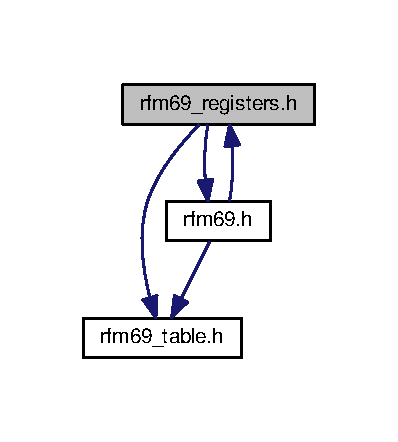
\includegraphics[width=191pt]{rfm69__registers_8h__incl}
\end{center}
\end{figure}
Граф файлов, в которые включается этот файл\+:
\nopagebreak
\begin{figure}[H]
\begin{center}
\leavevmode
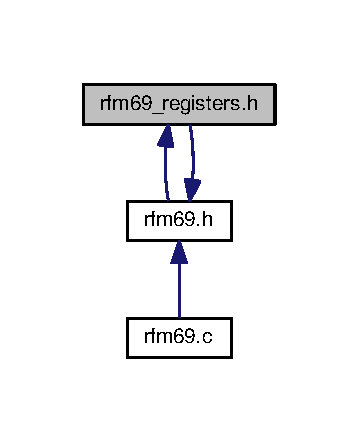
\includegraphics[width=172pt]{rfm69__registers_8h__dep__incl}
\end{center}
\end{figure}
\subsection*{Макросы}
\begin{DoxyCompactItemize}
\item 
\#define \hyperlink{rfm69__registers_8h_a20ec1927b7f8bef2f0e096b2e241d749}{R\+E\+G\+F\+I\+F\+O}~0x00
\item 
\#define \hyperlink{rfm69__registers_8h_a725aadf224f762f20fd93bfc3edcbb76}{R\+E\+G\+O\+P\+M\+O\+D\+E}~0x01
\item 
\#define \hyperlink{rfm69__registers_8h_ad34e500db60585f5c256b04bd898ebba}{S\+E\+Q\+U\+E\+N\+C\+E\+R\+O\+F\+F}~7
\item 
\#define \hyperlink{rfm69__registers_8h_ac873ed4655b1b8770ef2994e5c02c5d7}{L\+I\+S\+T\+E\+N\+O\+N}~6
\item 
\#define \hyperlink{rfm69__registers_8h_a4f6f5d1b390ad4a277eade9bb426bfa2}{L\+I\+S\+T\+E\+N\+A\+B\+O\+R\+T}~5
\item 
\#define \hyperlink{rfm69__registers_8h_aca1f7e0907b7f07b7ea6ddbe8fac6ac5}{R\+X\+\_\+\+M\+O\+D\+E}~0x10
\item 
\#define \hyperlink{rfm69__registers_8h_a60bcaae69589922d624e3a7c1cedd686}{T\+X\+\_\+\+M\+O\+D\+E}~0x0c
\item 
\#define \hyperlink{rfm69__registers_8h_a03829d3a0bcb79ea69d359c0e23b7a43}{F\+S\+\_\+\+M\+O\+D\+E}~0x08
\item 
\#define \hyperlink{rfm69__registers_8h_a706e8f23c905d8e9c63fe75c5a74d462}{S\+T\+B\+Y\+\_\+\+M\+O\+D\+E}~0x04
\item 
\#define \hyperlink{rfm69__registers_8h_a6097218fc13c9936e96507d6fd9fafe0}{S\+L\+E\+E\+P\+\_\+\+M\+O\+D\+E}~0x00
\item 
\#define \hyperlink{rfm69__registers_8h_a11e8550da335f8b4ae8b85c5c2db4921}{R\+E\+G\+D\+A\+T\+A\+M\+O\+D\+U\+L}~0x02
\item 
\#define \hyperlink{rfm69__registers_8h_ac08f2c3736cc23fc9d36d95d4f6a205f}{C\+O\+N\+T\+\_\+\+M\+O\+D\+E}~0x60
\item 
\#define \hyperlink{rfm69__registers_8h_a720d690ab49854e6eb434d2c2ede8e24}{C\+O\+N\+T\+\_\+\+S\+Y\+N\+C\+H\+\_\+\+M\+O\+D\+E}~0x40
\item 
\#define \hyperlink{rfm69__registers_8h_a366d2e1ca64909f289bde16361b6fd07}{P\+A\+C\+K\+E\+T\+\_\+\+M\+O\+D\+E}~0x00
\item 
\#define \hyperlink{rfm69__registers_8h_ab69783dc911fb5e872ee21543a3bc23f}{G\+A\+U\+S\+S\+\_\+\+B\+T03}~0x03
\item 
\#define \hyperlink{rfm69__registers_8h_a2fa9dc5e3fc4742b46551703ba1c9500}{G\+A\+U\+S\+S\+\_\+\+B\+T05}~0x02
\item 
\#define \hyperlink{rfm69__registers_8h_a4a70bc27906df4705fba032b0bcec59b}{G\+A\+U\+S\+S\+\_\+\+B\+T10}~0x01
\item 
\#define \hyperlink{rfm69__registers_8h_a4ce846d2651bdbbabc166ea0603902d6}{N\+O\+\_\+\+S\+H\+A\+P\+I\+N\+G}~0x00
\item 
\#define \hyperlink{rfm69__registers_8h_a097e1638f022624c30fb2a99e2230325}{R\+E\+G\+B\+I\+T\+R\+A\+T\+E\+M\+S\+B}~0x03
\item 
\#define \hyperlink{rfm69__registers_8h_a8a8aeb284eaba32c7f413543988d8fde}{R\+E\+G\+B\+I\+T\+R\+A\+T\+E\+L\+S\+B}~0x04
\item 
\#define \hyperlink{rfm69__registers_8h_ac1ae7970d0dcf267a7a5ca51687d97fe}{B\+I\+T\+R\+A\+T\+E\+\_\+\+C\+A\+L\+C}(br\+\_\+par)~\hyperlink{rfm69_8h_a108423b4512abbd8ed01ddfe33955fd4}{F\+X\+O\+S\+C}/(br\+\_\+par)
\item 
\#define \hyperlink{rfm69__registers_8h_a61b5340a670344fef34a246193f7260a}{R\+E\+G\+F\+D\+E\+V\+M\+S\+B}~0x05
\item 
\#define \hyperlink{rfm69__registers_8h_a0fde08a8331c90bb87675ed0f5c694d7}{R\+E\+G\+F\+D\+E\+V\+L\+S\+B}~0x06
\item 
\#define \hyperlink{rfm69__registers_8h_a77666bfe5e6e90bb35003fa957f9ec6f}{F\+D\+E\+V\+\_\+\+C\+A\+L\+C}(fdev\+\_\+par)~(fdev\+\_\+par)/\hyperlink{rfm69_8h_aef5e22694322d48a9607f13bb9a4c6f4}{F\+S\+T\+E\+P}
\item 
\#define \hyperlink{rfm69__registers_8h_a2d4455b84d3bb31e9037664d84114c26}{R\+E\+G\+F\+R\+F\+M\+S\+B}~0x07
\item 
\#define \hyperlink{rfm69__registers_8h_a09a33074e73ae38230fec3a5783395a9}{R\+E\+G\+F\+R\+F\+M\+I\+D}~0x08
\item 
\#define \hyperlink{rfm69__registers_8h_a6dd2f58496f2d15c8a0a388f75301023}{R\+E\+G\+F\+R\+F\+L\+S\+B}~0x09
\item 
\#define \hyperlink{rfm69__registers_8h_ae902e7a3545149f07d33ebeea9e3ba11}{F\+R\+F\+\_\+\+C\+A\+L\+C}(frf\+\_\+par)~(frf\+\_\+par)/\hyperlink{rfm69_8h_aef5e22694322d48a9607f13bb9a4c6f4}{F\+S\+T\+E\+P}
\item 
\#define \hyperlink{rfm69__registers_8h_a9ab2d8a0684900022d9a84ff558ee5e2}{R\+E\+G\+O\+S\+C1}~0x0a
\item 
\#define \hyperlink{rfm69__registers_8h_ae462be44633b786c55de7007403a379f}{R\+C\+C\+A\+L\+S\+T\+A\+R\+T}~7
\item 
\#define \hyperlink{rfm69__registers_8h_a8922110741ed3478468f73162cfc1a6d}{R\+C\+C\+A\+L\+D\+O\+N\+E}~6
\item 
\#define \hyperlink{rfm69__registers_8h_a9b83d33f4777a793bd16609f717b7082}{R\+E\+G\+A\+F\+C\+C\+T\+R\+L}~0x0b
\item 
\#define \hyperlink{rfm69__registers_8h_ad5d2eba8b4963a97848a746ba9094346}{A\+F\+C\+L\+O\+W\+B\+E\+T\+A\+O\+N}~5
\item 
\#define \hyperlink{rfm69__registers_8h_a71306bd3eec974fa3ada43b3e2dbdd35}{R\+E\+G\+L\+I\+S\+T\+E\+N1}~0x0d
\item 
\#define \hyperlink{rfm69__registers_8h_a57f032180697bcacf5b20f7a38af99a3}{L\+I\+S\+T\+E\+N\+I\+D\+L\+E262\+M}~0xc0
\item 
\#define \hyperlink{rfm69__registers_8h_a5b70af578773aa3acd705cf6d85498f6}{L\+I\+S\+T\+E\+N\+I\+D\+L\+E4\+M1}~0x80
\item 
\#define \hyperlink{rfm69__registers_8h_a3b3e093a7843affae6faf2bbcc739be5}{L\+I\+S\+T\+E\+N\+I\+D\+L\+E64\+U}~0x40
\item 
\#define \hyperlink{rfm69__registers_8h_a6cb137d5e823989e7689476ea73a5cc2}{L\+I\+S\+T\+E\+N\+R\+X262\+M}~0x30
\item 
\#define \hyperlink{rfm69__registers_8h_a58f75f5c4cedd4218ef0dc5c04a64126}{L\+I\+S\+T\+E\+N\+R\+X4\+M1}~0x20
\item 
\#define \hyperlink{rfm69__registers_8h_a2f45a4ab81593661a3292463c086458e}{L\+I\+S\+T\+E\+N\+R\+X64\+U}~0x10
\item 
\#define \hyperlink{rfm69__registers_8h_a0b72ec5c1408de14cd281ad7ee3d0c19}{L\+I\+S\+T\+E\+N\+C\+R\+I\+T\+E\+R\+I\+A}~3
\item 
\#define \hyperlink{rfm69__registers_8h_a8115466d2e70941b52432eee7a51d4f4}{L\+I\+S\+T\+E\+N\+E\+N\+D1}~0x00
\item 
\#define \hyperlink{rfm69__registers_8h_a1883b06541fa927c7aeab7074de4f209}{L\+I\+S\+T\+E\+N\+E\+N\+D2}~0x02
\item 
\#define \hyperlink{rfm69__registers_8h_ae80469e5b55ea62811140ba203331c18}{L\+I\+S\+T\+E\+N\+E\+N\+D3}~0x04
\item 
\#define \hyperlink{rfm69__registers_8h_a9ddae3ddaa84bf43fa2d22d9b7ff982f}{L\+I\+S\+T\+E\+N\+E\+N\+D4}~0x06
\item 
\#define \hyperlink{rfm69__registers_8h_a0578317a8618587883d8b137310fdc44}{R\+E\+G\+L\+I\+S\+T\+E\+N2}~0x0e
\item 
\#define \hyperlink{rfm69__registers_8h_a591993b8a74af8cc8a56baa3aa0880ee}{R\+E\+G\+L\+I\+S\+T\+E\+N3}~0x0f
\item 
\#define \hyperlink{rfm69__registers_8h_ac7860f81933f078c6ec0a6fc60a11a6a}{R\+E\+G\+V\+E\+R\+S\+I\+O\+N}~0x10
\item 
\#define \hyperlink{rfm69__registers_8h_ab846b1273c96f70c1a4d44c1c06f744f}{R\+E\+G\+P\+A\+L\+E\+V\+E\+L}~0x11
\item 
\#define \hyperlink{rfm69__registers_8h_a1349892a7adac828df5ab3a395e557e0}{P\+A0\+O\+N}~7
\item 
\#define \hyperlink{rfm69__registers_8h_a0048b53a5557ee80b7792fde9f976ba5}{P\+A1\+O\+N}~6
\item 
\#define \hyperlink{rfm69__registers_8h_ae5a87eb57ec917fd5b5fe4083875e19a}{P\+A2\+O\+N}~5
\item 
\#define \hyperlink{rfm69__registers_8h_acb5c8c4439d716b93a8d4767ac398e60}{O\+U\+T\+\_\+\+P\+O\+W\+E\+R\+\_\+\+C\+A\+L\+C}(power\+\_\+par)~0x1f\&(18 + (power\+\_\+par))
\item 
\#define \hyperlink{rfm69__registers_8h_a1d32019f8d7bdfc812efc3b4159465be}{R\+E\+G\+P\+A\+R\+A\+M\+P}~0x12
\item 
\#define \hyperlink{rfm69__registers_8h_adb13d996270e7b3405f50af85c397922}{R\+E\+G\+O\+C\+P}~0x13
\item 
\#define \hyperlink{rfm69__registers_8h_a241fa810dd7c750734cf4d02893a8aaf}{O\+C\+P\+O\+N}~4
\item 
\#define \hyperlink{rfm69__registers_8h_aedcc657b574a4c9f7956f94ad2e65d4a}{O\+C\+P\+\_\+\+C\+U\+R\+R\+E\+N\+T\+\_\+\+C\+A\+L\+C}(ocp\+\_\+param)~0x0f\&(((ocp\+\_\+param)/5) -\/ 9)
\item 
\#define \hyperlink{rfm69__registers_8h_a124c0f8478c91b94f395a12f1900dd98}{R\+E\+G\+L\+N\+A}~0x18
\item 
\#define \hyperlink{rfm69__registers_8h_a95610ecbca4757054e9becc0f6da8001}{L\+N\+A\+Z\+I\+N}~7
\item 
\#define \hyperlink{rfm69__registers_8h_a49a78405e3eb02eaf9ffc105a608f478}{L\+N\+A\+G\+A\+I\+N\+\_\+\+A\+U\+T\+O}~0x00
\item 
\#define \hyperlink{rfm69__registers_8h_a84873bed84b9340fea0f0efa2f530413}{L\+N\+A\+G\+A\+I\+N\+\_\+0\+D\+B}~0x01
\item 
\#define \hyperlink{rfm69__registers_8h_a7c479aca2d55a39ce6ea29b19e049fee}{L\+N\+A\+G\+A\+I\+N\+\_\+6\+D\+B}~0x02
\item 
\#define \hyperlink{rfm69__registers_8h_abec8e8899abb8676e271a393dc71e4cc}{L\+N\+A\+G\+A\+I\+N\+\_\+12\+D\+B}~0x03
\item 
\#define \hyperlink{rfm69__registers_8h_a4f5bbac109b2fb500f51e37a9e8e5584}{L\+N\+A\+G\+A\+I\+N\+\_\+24\+D\+B}~0x04
\item 
\#define \hyperlink{rfm69__registers_8h_abd10dd2297d2d315c17627f73472de17}{L\+N\+A\+G\+A\+I\+N\+\_\+36\+D\+B}~0x05
\item 
\#define \hyperlink{rfm69__registers_8h_ac2b74f9b02bba028a47c3cca0963e641}{L\+N\+A\+G\+A\+I\+N\+\_\+48\+D\+B}~0x06
\item 
\#define \hyperlink{rfm69__registers_8h_a04d948dfd6c111a781e9d4faff096ddc}{R\+E\+G\+R\+X\+B\+W}~0x19
\item 
\#define \hyperlink{rfm69__registers_8h_a3618990d81a06a7579a4235ba9087c7b}{R\+E\+G\+A\+F\+C\+B\+W}~0x1a
\item 
\#define \hyperlink{rfm69__registers_8h_a7551afc713c923527a9e440621453ed1}{R\+E\+G\+O\+O\+K\+P\+E\+A\+K}~0x1b
\item 
\#define \hyperlink{rfm69__registers_8h_aeff2ccb27679b8484f8e026c43245589}{O\+O\+K\+T\+H\+R\+E\+S\+F\+I\+X\+E\+D}~0x00
\item 
\#define \hyperlink{rfm69__registers_8h_a1f168d02ead502f19915a4d30f65af5a}{O\+O\+K\+T\+H\+R\+E\+S\+P\+E\+A\+K}~0x40
\item 
\#define \hyperlink{rfm69__registers_8h_af212a794e44077811e9d17865b9e7615}{O\+O\+K\+T\+H\+R\+E\+S\+A\+V\+E\+R\+A\+G\+E}~0x80
\item 
\#define \hyperlink{rfm69__registers_8h_a1e7581c4ffcbed58604c591226e4d978}{R\+E\+G\+O\+O\+K\+A\+V\+G}~0x1c
\item 
\#define \hyperlink{rfm69__registers_8h_a0aa0e89486d7839ba9c4e84c65fae7bd}{R\+E\+G\+O\+O\+K\+F\+I\+X}~0x1d
\item 
\#define \hyperlink{rfm69__registers_8h_a549146031e910654195343941b259b4a}{R\+E\+G\+A\+F\+C\+F\+E\+I}~0x1e
\item 
\#define \hyperlink{rfm69__registers_8h_ae62e1cd7f99a669aace9977a00223e04}{F\+E\+I\+D\+O\+N\+E}~6
\item 
\#define \hyperlink{rfm69__registers_8h_a5ef3181e5a9fd8907344932012b2dc06}{F\+E\+I\+S\+T\+A\+R\+T}~5
\item 
\#define \hyperlink{rfm69__registers_8h_a89c452b62e13a82d037b2b55e5618781}{A\+F\+C\+D\+O\+N\+E}~4
\item 
\#define \hyperlink{rfm69__registers_8h_ac3f3f8de47d947af91e9b12e8a461e2c}{A\+F\+C\+A\+U\+T\+O\+C\+L\+E\+A\+R}~3
\item 
\#define \hyperlink{rfm69__registers_8h_ab65fcdba5953290d2b432eab78862c90}{A\+F\+C\+A\+U\+T\+O\+O\+N}~2
\item 
\#define \hyperlink{rfm69__registers_8h_a743e57d19924300e6a03ed29ca842378}{A\+F\+C\+C\+L\+E\+A\+R}~1
\item 
\#define \hyperlink{rfm69__registers_8h_a530b80f625c918cd513e806690c3eb8f}{A\+F\+C\+S\+T\+A\+R\+T}~0
\item 
\#define \hyperlink{rfm69__registers_8h_ae1d8204973c4f035a2531a49399932bc}{R\+E\+G\+A\+F\+C\+M\+S\+B}~0x1f
\item 
\#define \hyperlink{rfm69__registers_8h_a30bb86310fbf89c247c1d7633ac3d5fd}{R\+E\+G\+A\+F\+C\+L\+S\+B}~0x20
\item 
\#define \hyperlink{rfm69__registers_8h_a978731b8f67ea668b31cd6ebbce46438}{A\+F\+C\+\_\+\+V\+A\+L\+U\+E}(afc\+\_\+par)~(afc\+\_\+par)$\ast$\hyperlink{rfm69_8h_aef5e22694322d48a9607f13bb9a4c6f4}{F\+S\+T\+E\+P}
\item 
\#define \hyperlink{rfm69__registers_8h_a8173b0c23d1021f13568f8361c16d688}{R\+E\+G\+F\+E\+I\+M\+S\+B}~0x21
\item 
\#define \hyperlink{rfm69__registers_8h_a8911f63976ee2fc01359a23a4006c6a0}{R\+E\+G\+F\+E\+I\+L\+S\+B}~0x22
\item 
\#define \hyperlink{rfm69__registers_8h_ac372489905bd18f905f1bbaed3567bd2}{F\+E\+I\+\_\+\+V\+A\+L\+U\+E}(fei\+\_\+par)~(fei\+\_\+par)$\ast$\hyperlink{rfm69_8h_aef5e22694322d48a9607f13bb9a4c6f4}{F\+S\+T\+E\+P}
\item 
\#define \hyperlink{rfm69__registers_8h_a1bb435143f57d8ec7f961485ff1fd2f8}{R\+E\+G\+R\+S\+S\+I\+C\+O\+N\+F\+I\+G}~0x23
\item 
\#define \hyperlink{rfm69__registers_8h_a5c3ca15b347688880a2060b702b4008a}{R\+S\+S\+I\+D\+O\+N\+E}~1
\item 
\#define \hyperlink{rfm69__registers_8h_a4b107df1798a385cc8351847f6e74732}{R\+S\+S\+I\+S\+T\+A\+R\+T}~0
\item 
\#define \hyperlink{rfm69__registers_8h_a056390289d6aa9905db0fdbf661547c1}{R\+E\+G\+R\+S\+S\+I\+V\+A\+L\+U\+E}~0x24
\item 
\#define \hyperlink{rfm69__registers_8h_af2bca333b4f95258231d7f991e6e5f4a}{R\+S\+S\+I\+\_\+\+V\+A\+L\+U\+E}(rssi\+\_\+par)~(rssi\+\_\+par)/2
\item 
\#define \hyperlink{rfm69__registers_8h_ae2cf028d3c2b1a9ebf20e044888afe9e}{R\+E\+G\+D\+I\+O\+M\+A\+P\+P\+I\+N\+G1}~0x25
\item 
\#define \hyperlink{rfm69__registers_8h_a4f3496e7ca63e021951eb2710254afa1}{D\+I\+O0\+M\+A\+P0}~0x00
\item 
\#define \hyperlink{rfm69__registers_8h_ae813cfcd6751615ac9bcab14078f75e2}{D\+I\+O0\+M\+A\+P1}~0x40
\item 
\#define \hyperlink{rfm69__registers_8h_a1e22c2bc2823cccc33777c8522d36bba}{D\+I\+O0\+M\+A\+P2}~0x80
\item 
\#define \hyperlink{rfm69__registers_8h_a47c2b7e0dd8a83495dcef623d28f6f16}{D\+I\+O0\+M\+A\+P3}~0xc0
\item 
\#define \hyperlink{rfm69__registers_8h_a45c774244e4f9ecc7b74c3d27c3c9e25}{D\+I\+O1\+M\+A\+P0}~0x00
\item 
\#define \hyperlink{rfm69__registers_8h_a28dbdd3048a49e9534c5353c78041746}{D\+I\+O1\+M\+A\+P1}~0x10
\item 
\#define \hyperlink{rfm69__registers_8h_a6768e5f5ad9ec28893d234ec785fffa1}{D\+I\+O1\+M\+A\+P2}~0x20
\item 
\#define \hyperlink{rfm69__registers_8h_a81410d3fd6bef577f3a249ffecbd6786}{D\+I\+O1\+M\+A\+P3}~0x30
\item 
\#define \hyperlink{rfm69__registers_8h_aed2a21f1c1c6a797caba129bc9e4c0e8}{D\+I\+O2\+M\+A\+P0}~0x00
\item 
\#define \hyperlink{rfm69__registers_8h_ab2663f2f2c9f76826476ab37c9367c73}{D\+I\+O2\+M\+A\+P1}~0x04
\item 
\#define \hyperlink{rfm69__registers_8h_a3247a01dec1629f6cb03b84784d84bbe}{D\+I\+O2\+M\+A\+P2}~0x08
\item 
\#define \hyperlink{rfm69__registers_8h_a67d05e78726b0140d9871f9b2ad47135}{D\+I\+O2\+M\+A\+P3}~0x0c
\item 
\#define \hyperlink{rfm69__registers_8h_a847863754d98a5a67d2d6fa3b6144899}{D\+I\+O3\+M\+A\+P0}~0x00
\item 
\#define \hyperlink{rfm69__registers_8h_af9f9c18fc5ead63d4aaa535177542834}{D\+I\+O3\+M\+A\+P1}~0x01
\item 
\#define \hyperlink{rfm69__registers_8h_a3bc270a2d23e70b889bc46c84fbb976b}{D\+I\+O3\+M\+A\+P2}~0x02
\item 
\#define \hyperlink{rfm69__registers_8h_aa0a8add085e07f5041b9a69ed3ecf3b8}{D\+I\+O3\+M\+A\+P3}~0x03
\item 
\#define \hyperlink{rfm69__registers_8h_ae3223941a8a257b0df1eb6554b69430d}{R\+E\+G\+D\+I\+O\+M\+A\+P\+P\+I\+N\+G2}~0x26
\item 
\#define \hyperlink{rfm69__registers_8h_a72f94132418287bf937d1d3bbd4becb4}{D\+I\+O5\+M\+A\+P0}~0x00
\item 
\#define \hyperlink{rfm69__registers_8h_a6695cdbe35431feaa9093f833bde3e5f}{D\+I\+O5\+M\+A\+P1}~0x10
\item 
\#define \hyperlink{rfm69__registers_8h_a8f5e4e5bf7d65e3cee47c16c31a5bc6a}{D\+I\+O5\+M\+A\+P2}~0x20
\item 
\#define \hyperlink{rfm69__registers_8h_aaaa42b382c12ce1af8f984d86f0456e4}{D\+I\+O5\+M\+A\+P3}~0x30
\item 
\#define \hyperlink{rfm69__registers_8h_a11cfa96d484ace5ce257786f77580942}{C\+L\+K\+O\+U\+T32\+M}~0x00
\item 
\#define \hyperlink{rfm69__registers_8h_a79b499b028888bc8c6dacfe9b829eecf}{C\+L\+K\+O\+U\+T16\+M}~0x01
\item 
\#define \hyperlink{rfm69__registers_8h_ac9da285bce38f36312291a81815b7f09}{C\+L\+K\+O\+U\+T8\+M}~0x02
\item 
\#define \hyperlink{rfm69__registers_8h_a00266508cf870890e84f276c44c1ece8}{C\+L\+K\+O\+U\+T4\+M}~0x03
\item 
\#define \hyperlink{rfm69__registers_8h_a410e776f61c135095dae973755d6727d}{C\+L\+K\+O\+U\+T2\+M}~0x04
\item 
\#define \hyperlink{rfm69__registers_8h_af32325a419e074ab0960dfaf8a8e693c}{C\+L\+K\+O\+U\+T1\+M}~0x05
\item 
\#define \hyperlink{rfm69__registers_8h_a7657be8bf90f441396837442586c0221}{C\+L\+K\+O\+U\+T\+\_\+\+R\+C}~0x06
\item 
\#define \hyperlink{rfm69__registers_8h_a55de476fb11aadcf3811e2d98442bb79}{C\+L\+K\+O\+U\+T\+\_\+\+O\+F\+F}~0x07
\item 
\#define \hyperlink{rfm69__registers_8h_a5581bc34e2146c8800315d45db1dff95}{R\+E\+G\+I\+R\+Q\+F\+L\+A\+G\+S1}~0x27
\item 
\#define \hyperlink{rfm69__registers_8h_a92cb4444110d68c98094440cdac68967}{M\+O\+D\+E\+R\+E\+A\+D\+Y}~7
\item 
\#define \hyperlink{rfm69__registers_8h_a9a5efc560263b8ce73d05900de6b389c}{R\+X\+R\+E\+A\+D\+Y}~6
\item 
\#define \hyperlink{rfm69__registers_8h_a10384620cdac74aee8dafcca97f6159d}{T\+X\+R\+E\+A\+D\+Y}~5
\item 
\#define \hyperlink{rfm69__registers_8h_a1cdc3c070e5a5522a7e604bce088e265}{P\+L\+L\+L\+O\+C\+K}~4
\item 
\#define \hyperlink{rfm69__registers_8h_a2e5f67a52331dcf76b9d8322689966d8}{R\+S\+S\+I\+\_\+\+I}~3
\item 
\#define \hyperlink{rfm69__registers_8h_a45ba202b05caf39795aeca91b0ae547e}{T\+I\+M\+E\+O\+U\+T}~2
\item 
\#define \hyperlink{rfm69__registers_8h_ac695544d945cf9327cdeb1c7634f85b5}{A\+U\+T\+O\+M\+O\+D\+E}~1
\item 
\#define \hyperlink{rfm69__registers_8h_a17a1cea93e6f57035eaae10f7333076f}{S\+Y\+N\+C\+A\+D\+D\+R\+M\+A\+T\+C\+H}~0
\item 
\#define \hyperlink{rfm69__registers_8h_ad70e04845dd0a9881a85998903e22f18}{R\+E\+G\+I\+R\+Q\+F\+L\+A\+G\+S2}~0x28
\item 
\#define \hyperlink{rfm69__registers_8h_a77aff42ee63cba9ce0da81cea1a6d31a}{F\+I\+F\+O\+I\+S\+F\+U\+L\+L}~7
\item 
\#define \hyperlink{rfm69__registers_8h_a171aa0f0eeeba7bc44c1516a4c17f1a9}{F\+I\+F\+O\+N\+O\+T\+E\+M\+P\+T\+Y}~6
\item 
\#define \hyperlink{rfm69__registers_8h_a91beafaa9e1bd277c49133dacc35dfac}{F\+I\+F\+O\+L\+E\+V\+E\+L}~5
\item 
\#define \hyperlink{rfm69__registers_8h_a6ca169e1b9cd5a6722cafceb80991e85}{F\+I\+F\+O\+O\+V\+E\+R\+R\+U\+N}~4
\item 
\#define \hyperlink{rfm69__registers_8h_ab94ae9d0a96f994c152c3f63abca6024}{P\+A\+C\+K\+E\+T\+S\+E\+N\+T}~3
\item 
\#define \hyperlink{rfm69__registers_8h_acb819e9cd3dc27e3becd01e8354ddf2f}{P\+A\+Y\+L\+O\+A\+D\+R\+E\+A\+D\+Y}~2
\item 
\#define \hyperlink{rfm69__registers_8h_ac42f89172030ef27658293ddadfd07a1}{C\+R\+C\+O\+K}~1
\item 
\#define \hyperlink{rfm69__registers_8h_ad8096e614a46fa1f7bf4f9f4d27c318b}{R\+E\+G\+R\+S\+S\+I\+T\+H\+R\+E\+S\+H}~0x29
\item 
\#define \hyperlink{rfm69__registers_8h_aab1351f68c4bd1865fae376734674afd}{R\+S\+S\+I\+\_\+\+T\+H\+R\+E\+S\+H\+\_\+\+C\+A\+L\+C}(rssi\+\_\+parr)~(rssi\+\_\+parr)$\ast$2
\item 
\#define \hyperlink{rfm69__registers_8h_a011c4501e15a8911eda75ac89d58018b}{R\+E\+G\+R\+X\+T\+I\+M\+E\+O\+U\+T1}~0x2a
\item 
\#define \hyperlink{rfm69__registers_8h_adc87e99d3b958b525723983049f150f0}{R\+E\+G\+R\+X\+T\+I\+M\+E\+O\+U\+T2}~0x2b
\item 
\#define \hyperlink{rfm69__registers_8h_ad2eeeec32f8cfd2cdec89fc174a95b71}{R\+E\+G\+P\+R\+E\+A\+M\+B\+L\+E\+M\+S\+B}~0x2c
\item 
\#define \hyperlink{rfm69__registers_8h_a93c96ac4c17b088f5a6594522827b3cc}{R\+E\+G\+P\+R\+E\+A\+M\+B\+L\+E\+L\+S\+B}~0x2d
\item 
\#define \hyperlink{rfm69__registers_8h_a2bc1333738c0815e521613938a5498dc}{R\+E\+G\+S\+Y\+N\+C\+C\+O\+N\+F\+I\+G}~0x2e
\item 
\#define \hyperlink{rfm69__registers_8h_a5a8ee3bc363c8cdf8acb30fcef379b1b}{S\+Y\+N\+C\+O\+N}~7
\item 
\#define \hyperlink{rfm69__registers_8h_ad5136933340ac95954fc304b58fc005c}{F\+I\+F\+O\+F\+I\+L\+L\+C\+O\+N\+D}~6
\item 
\#define \hyperlink{rfm69__registers_8h_acd179fc969c2f0e41b6bd5e1aa7906f1}{S\+Y\+N\+C\+S\+I\+Z\+E\+\_\+\+C\+A\+L\+C}(syncsize\+\_\+par)~( (( (syncsize\+\_\+par) -\/ 1 ) \& 0x07) $<$$<$ 3 )
\item 
\#define \hyperlink{rfm69__registers_8h_ae106483494497c8026ab22e1ef8fcdf6}{S\+Y\+N\+C\+\_\+\+W\+O\+R\+D\+\_\+\+O\+N}~0x80
\item 
\#define \hyperlink{rfm69__registers_8h_a6ee2457b4f576c698411cb0ab894db9b}{R\+E\+G\+S\+Y\+N\+C\+V\+A\+L\+U\+E1}~0x2f
\item 
\#define \hyperlink{rfm69__registers_8h_adaca8600b14d05a9c040f41fa138f1d8}{R\+E\+G\+S\+Y\+N\+C\+V\+A\+L\+U\+E2}~0x30
\item 
\#define \hyperlink{rfm69__registers_8h_a72799d7522e3cf5eab70330ae5ea18f5}{R\+E\+G\+S\+Y\+N\+C\+V\+A\+L\+U\+E3}~0x31
\item 
\#define \hyperlink{rfm69__registers_8h_af73cec688464a1a876c1537b2a2c1585}{R\+E\+G\+S\+Y\+N\+C\+V\+A\+L\+U\+E4}~0x32
\item 
\#define \hyperlink{rfm69__registers_8h_a7f56f21a74bacdb62ca3c56f8460f15b}{R\+E\+G\+S\+Y\+N\+C\+V\+A\+L\+U\+E5}~0x33
\item 
\#define \hyperlink{rfm69__registers_8h_a5bfe98591e912a4d3ebcba3ee86510e2}{R\+E\+G\+S\+Y\+N\+C\+V\+A\+L\+U\+E6}~0x34
\item 
\#define \hyperlink{rfm69__registers_8h_a55fce655cb8a811fbd5784b344404d2a}{R\+E\+G\+S\+Y\+N\+C\+V\+A\+L\+U\+E7}~0x35
\item 
\#define \hyperlink{rfm69__registers_8h_a9c05432f6eeff13f8b28eb3b1da71ae2}{R\+E\+G\+S\+Y\+N\+C\+V\+A\+L\+U\+E8}~0x36
\item 
\#define \hyperlink{rfm69__registers_8h_a4b11f6a06f72fab02a3560d3f6cc0926}{R\+E\+G\+P\+A\+C\+K\+E\+T\+C\+O\+N\+F\+I\+G1}~0x37
\item 
\#define \hyperlink{rfm69__registers_8h_a5db0212961ff5494d1c9d6efdcf03730}{P\+A\+C\+K\+E\+T\+F\+O\+R\+M\+A\+T}~7
\item 
\#define \hyperlink{rfm69__registers_8h_a15df7bdfa2cb6787bd141aefc0f93e12}{E\+N\+C\+O\+D\+I\+N\+G\+\_\+\+O\+F\+F}~0x00
\item 
\#define \hyperlink{rfm69__registers_8h_a120283fb693b8422442adc2efd40c388}{M\+A\+N\+C\+H\+E\+S\+T\+E\+R\+\_\+\+E\+N\+C}~0x20
\item 
\#define \hyperlink{rfm69__registers_8h_a304305da7043606cd4dd1beea9b89ab1}{D\+A\+T\+A\+\_\+\+W\+H\+I\+T\+E\+N\+I\+N\+G}~0x40
\item 
\#define \hyperlink{rfm69__registers_8h_a73c706d20d14f72e4864392b4bad9799}{C\+R\+C\+O\+N}~4
\item 
\#define \hyperlink{rfm69__registers_8h_ad5bfb4aedaab8eef409e4e7838caa375}{C\+R\+C\+A\+U\+T\+O\+C\+L\+E\+A\+R\+O\+F\+F}~3
\item 
\#define \hyperlink{rfm69__registers_8h_a4dfbb7041e66090274f3d17e36e8d31c}{A\+D\+D\+R\+E\+S\+S\+\_\+\+O\+F\+F}~0x00
\item 
\#define \hyperlink{rfm69__registers_8h_a34bddadd70544f1ca99813d4b1cea8f4}{N\+O\+D\+E\+\_\+\+A\+D\+D\+R\+E\+S\+S\+\_\+\+O\+N\+L\+Y}~0x02
\item 
\#define \hyperlink{rfm69__registers_8h_ab3f7692a1ea401ba18ca18246ebef425}{N\+O\+D\+E\+\_\+\+B\+R\+O\+A\+D\+C\+A\+S\+T\+\_\+\+A\+D\+D\+R}~0\+X04
\item 
\#define \hyperlink{rfm69__registers_8h_abffe757f637526671e8e20fcdbdec770}{R\+E\+G\+P\+A\+Y\+L\+O\+A\+D\+L\+E\+N\+G\+H\+T}~0x38
\item 
\#define \hyperlink{rfm69__registers_8h_a4b29fab9c29e60f09b04d5a0f605b189}{R\+E\+G\+N\+O\+D\+E\+A\+D\+R\+S}~0x39
\item 
\#define \hyperlink{rfm69__registers_8h_a4d662c8cda512fe543375ac7f6c46749}{R\+E\+G\+B\+R\+O\+A\+D\+C\+A\+S\+T\+A\+D\+R\+S}~0x3a
\item 
\#define \hyperlink{rfm69__registers_8h_a720271cffe57b38268a7ee7855973f9b}{R\+E\+G\+A\+U\+T\+O\+M\+O\+D\+E\+S}~0x3b
\item 
\#define \hyperlink{rfm69__registers_8h_a5cbc437168622c4aaa88c8903c426607}{R\+E\+G\+F\+I\+F\+O\+T\+H\+R\+E\+S}~0x3c
\item 
\#define \hyperlink{rfm69__registers_8h_a7500b77df8de3795a4eb235ed24c70f3}{T\+X\+S\+T\+A\+R\+T\+C\+O\+N\+D}~7
\item 
\#define \hyperlink{rfm69__registers_8h_a8ab30718fe278146f00e300a4c414055}{R\+E\+G\+P\+A\+C\+K\+E\+T\+C\+O\+N\+F\+I\+G2}~0x3d
\item 
\#define \hyperlink{rfm69__registers_8h_a22be40f300669af489a4c30c46e2d5ef}{R\+E\+S\+T\+A\+R\+T\+R\+X}~2
\item 
\#define \hyperlink{rfm69__registers_8h_a2056d2ccf745e838f1436ce70d8e81ff}{A\+U\+T\+O\+R\+X\+R\+E\+S\+T\+A\+R\+T\+O\+N}~1
\item 
\#define \hyperlink{rfm69__registers_8h_a329c471460a05db1a3cfb2c357465529}{A\+E\+S\+O\+N}~0
\item 
\#define \hyperlink{rfm69__registers_8h_af141e7eb7199de42b5f4bbd5ae07cd7c}{R\+E\+G\+A\+E\+S\+K\+E\+Y1}~0x3e
\item 
\#define \hyperlink{rfm69__registers_8h_aca6b34933f77bc9ef4cef51f55d68442}{R\+E\+G\+A\+E\+S\+K\+E\+Y2}~0x3f
\item 
\#define \hyperlink{rfm69__registers_8h_a9d5d17a8025ae0fec24dccfa0e5efadc}{R\+E\+G\+A\+E\+S\+K\+E\+Y3}~0x40
\item 
\#define \hyperlink{rfm69__registers_8h_a215e30e552e140bf1b5a0be60c799722}{R\+E\+G\+A\+E\+S\+K\+E\+Y4}~0x41
\item 
\#define \hyperlink{rfm69__registers_8h_aa9f9898119273eff104fa24d7209a2a0}{R\+E\+G\+A\+E\+S\+K\+E\+Y5}~0x42
\item 
\#define \hyperlink{rfm69__registers_8h_a9b76bda74c99e9ca6e09e1136744a43b}{R\+E\+G\+A\+E\+S\+K\+E\+Y6}~0x43
\item 
\#define \hyperlink{rfm69__registers_8h_a24a5fb2788fdd3e56a3a44560517aa0e}{R\+E\+G\+A\+E\+S\+K\+E\+Y7}~0x44
\item 
\#define \hyperlink{rfm69__registers_8h_ae61c54d55f736b51bd0576501717e76d}{R\+E\+G\+A\+E\+S\+K\+E\+Y8}~0x45
\item 
\#define \hyperlink{rfm69__registers_8h_a50f3c2dcec4fdb876a4a63ed79f5c750}{R\+E\+G\+A\+E\+S\+K\+E\+Y9}~0x46
\item 
\#define \hyperlink{rfm69__registers_8h_ae0b3f3ceb3f00370b451ec6edc0696fc}{R\+E\+G\+A\+E\+S\+K\+E\+Y10}~0x47
\item 
\#define \hyperlink{rfm69__registers_8h_a8afb4e59278ce7bb8965f96b2c549544}{R\+E\+G\+A\+E\+S\+K\+E\+Y11}~0x48
\item 
\#define \hyperlink{rfm69__registers_8h_a10e84f322d2d7dcaa4c992a29e078a97}{R\+E\+G\+A\+E\+S\+K\+E\+Y12}~0x49
\item 
\#define \hyperlink{rfm69__registers_8h_a00fa83f606f7ea91247127e0f2194dd8}{R\+E\+G\+A\+E\+S\+K\+E\+Y13}~0x4a
\item 
\#define \hyperlink{rfm69__registers_8h_adb3ced584661e9afb47fc1824ce695fd}{R\+E\+G\+A\+E\+S\+K\+E\+Y14}~0x4b
\item 
\#define \hyperlink{rfm69__registers_8h_a4afa53c6e54801cdbda901875b28f640}{R\+E\+G\+A\+E\+S\+K\+E\+Y15}~0x4c
\item 
\#define \hyperlink{rfm69__registers_8h_a80ac444c056692919e79d59f53f86e66}{R\+E\+G\+A\+E\+S\+K\+E\+Y16}~0x4d
\item 
\#define \hyperlink{rfm69__registers_8h_aa0bf8487f51a90f835e7c588f3f97b09}{R\+E\+G\+T\+E\+M\+P1}~0x4e
\item 
\#define \hyperlink{rfm69__registers_8h_a98f2faf0e85fee45baba3c2b454c6048}{T\+E\+M\+P\+M\+E\+A\+S\+S\+T\+A\+R\+T}~3
\item 
\#define \hyperlink{rfm69__registers_8h_a576ac61a926b2cdba9cefc2d46c679ec}{T\+E\+M\+P\+M\+E\+A\+S\+R\+U\+N\+N\+I\+N\+G}~2
\item 
\#define \hyperlink{rfm69__registers_8h_ae99e6d208b352bcde1a4cbdd0e703b6e}{R\+E\+G\+T\+E\+M\+P2}~0x4f
\item 
\#define \hyperlink{rfm69__registers_8h_a3f369b796fc94d07477b86e19c814684}{R\+E\+T\+E\+S\+T\+L\+N\+A}~0x58
\begin{DoxyCompactList}\small\item\em test registers \end{DoxyCompactList}\item 
\#define \hyperlink{rfm69__registers_8h_a422ea157d1233794520c913c10633a17}{N\+O\+R\+M\+A\+L\+\_\+\+S\+E\+N\+S\+\_\+\+B\+O\+O\+S\+T\+\_\+\+M\+O\+D\+E}~0x1b
\item 
\#define \hyperlink{rfm69__registers_8h_a2dd9a959b5e7b86f3db72b4adfe24f57}{H\+I\+G\+H\+\_\+\+S\+E\+N\+S\+\_\+\+B\+O\+O\+S\+T\+\_\+\+M\+O\+D\+E}~0x2d
\item 
\#define \hyperlink{rfm69__registers_8h_a31ce3ab758f3a942d93df2a0342e51f9}{R\+E\+G\+T\+E\+S\+T\+P\+A1}~0x5a
\item 
\#define \hyperlink{rfm69__registers_8h_ab5335091145d688a30c6a2156468964a}{P\+A1\+\_\+\+N\+O\+R\+M\+A\+L\+\_\+\+R\+X\+\_\+\+M\+O\+D\+E}~0x55
\item 
\#define \hyperlink{rfm69__registers_8h_a28f8253d94b542486ba3852172bb8362}{P\+A1\+\_\+13\+D\+B\+M\+\_\+\+R\+X\+\_\+\+M\+O\+D\+E}~0x5d
\item 
\#define \hyperlink{rfm69__registers_8h_a6b3b0e543c946639cb4593edfdf074eb}{P\+A1\+\_\+\+P\+A0\+\_\+\+O\+R\+\_\+\+R\+X}~0x55
\item 
\#define \hyperlink{rfm69__registers_8h_a4f6484d0d1a620c746c45706c7b4ac28}{R\+E\+G\+T\+E\+S\+T\+P\+A2}~0x5c
\item 
\#define \hyperlink{rfm69__registers_8h_a101c8ccb68669aacc8526d93bc30cb71}{P\+A2\+\_\+\+N\+O\+R\+M\+A\+L\+\_\+\+R\+X\+\_\+\+M\+O\+D\+E}~0x55
\item 
\#define \hyperlink{rfm69__registers_8h_a72b08315e4cf72629fbfd83c9653c1ad}{P\+A2\+\_\+13\+D\+B\+M\+\_\+\+R\+X\+\_\+\+M\+O\+D\+E}~0x5d
\item 
\#define \hyperlink{rfm69__registers_8h_ad0bf4cae65d5b154d4bdd1ec06ef3eb7}{P\+A2\+\_\+\+P\+A0\+\_\+\+O\+R\+\_\+\+R\+X}~0x55
\item 
\#define \hyperlink{rfm69__registers_8h_aed951ac28a32774019dbd38fb3da3ca7}{R\+E\+G\+T\+E\+S\+T\+D\+A\+G\+C}~0x6f
\item 
\#define \hyperlink{rfm69__registers_8h_a184a4c9e0bac911aaf2b3878c76cdada}{A\+F\+C\+\_\+\+N\+O\+R\+M\+A\+L\+\_\+\+M\+O\+D\+E}~0x00
\item 
\#define \hyperlink{rfm69__registers_8h_a5c79a9a0516fc19a9553557cc19e5204}{A\+F\+C\+\_\+\+L\+O\+W\+\_\+\+B\+E\+T\+A\+\_\+\+O\+N}~0x20
\item 
\#define \hyperlink{rfm69__registers_8h_a33856b4a4f7d1a963ce8e3bd598d83fb}{A\+F\+C\+\_\+\+L\+O\+W\+\_\+\+B\+E\+T\+A\+\_\+\+O\+F\+F}~0x30
\item 
\#define \hyperlink{rfm69__registers_8h_a41c186e401bd17378273ae58840a4f3c}{R\+E\+G\+T\+E\+S\+T\+A\+F\+C}~0x71
\item 
\#define \hyperlink{rfm69__registers_8h_a97d03ac0ed1b9277f0d3e9143275d20d}{L\+O\+W\+\_\+\+B\+E\+T\+A\+\_\+\+A\+F\+C\+\_\+\+O\+F\+F\+S\+E\+T\+\_\+\+C\+A\+L\+C}(afcoff\+\_\+par)~(afcoff\+\_\+par)$\ast$448
\end{DoxyCompactItemize}


\subsection{Макросы}
\hypertarget{rfm69__registers_8h_a4dfbb7041e66090274f3d17e36e8d31c}{\index{rfm69\+\_\+registers.\+h@{rfm69\+\_\+registers.\+h}!A\+D\+D\+R\+E\+S\+S\+\_\+\+O\+F\+F@{A\+D\+D\+R\+E\+S\+S\+\_\+\+O\+F\+F}}
\index{A\+D\+D\+R\+E\+S\+S\+\_\+\+O\+F\+F@{A\+D\+D\+R\+E\+S\+S\+\_\+\+O\+F\+F}!rfm69\+\_\+registers.\+h@{rfm69\+\_\+registers.\+h}}
\subsubsection[{A\+D\+D\+R\+E\+S\+S\+\_\+\+O\+F\+F}]{\setlength{\rightskip}{0pt plus 5cm}\#define A\+D\+D\+R\+E\+S\+S\+\_\+\+O\+F\+F~0x00}}\label{rfm69__registers_8h_a4dfbb7041e66090274f3d17e36e8d31c}
\hypertarget{rfm69__registers_8h_a329c471460a05db1a3cfb2c357465529}{\index{rfm69\+\_\+registers.\+h@{rfm69\+\_\+registers.\+h}!A\+E\+S\+O\+N@{A\+E\+S\+O\+N}}
\index{A\+E\+S\+O\+N@{A\+E\+S\+O\+N}!rfm69\+\_\+registers.\+h@{rfm69\+\_\+registers.\+h}}
\subsubsection[{A\+E\+S\+O\+N}]{\setlength{\rightskip}{0pt plus 5cm}\#define A\+E\+S\+O\+N~0}}\label{rfm69__registers_8h_a329c471460a05db1a3cfb2c357465529}
\hypertarget{rfm69__registers_8h_a33856b4a4f7d1a963ce8e3bd598d83fb}{\index{rfm69\+\_\+registers.\+h@{rfm69\+\_\+registers.\+h}!A\+F\+C\+\_\+\+L\+O\+W\+\_\+\+B\+E\+T\+A\+\_\+\+O\+F\+F@{A\+F\+C\+\_\+\+L\+O\+W\+\_\+\+B\+E\+T\+A\+\_\+\+O\+F\+F}}
\index{A\+F\+C\+\_\+\+L\+O\+W\+\_\+\+B\+E\+T\+A\+\_\+\+O\+F\+F@{A\+F\+C\+\_\+\+L\+O\+W\+\_\+\+B\+E\+T\+A\+\_\+\+O\+F\+F}!rfm69\+\_\+registers.\+h@{rfm69\+\_\+registers.\+h}}
\subsubsection[{A\+F\+C\+\_\+\+L\+O\+W\+\_\+\+B\+E\+T\+A\+\_\+\+O\+F\+F}]{\setlength{\rightskip}{0pt plus 5cm}\#define A\+F\+C\+\_\+\+L\+O\+W\+\_\+\+B\+E\+T\+A\+\_\+\+O\+F\+F~0x30}}\label{rfm69__registers_8h_a33856b4a4f7d1a963ce8e3bd598d83fb}
\hypertarget{rfm69__registers_8h_a5c79a9a0516fc19a9553557cc19e5204}{\index{rfm69\+\_\+registers.\+h@{rfm69\+\_\+registers.\+h}!A\+F\+C\+\_\+\+L\+O\+W\+\_\+\+B\+E\+T\+A\+\_\+\+O\+N@{A\+F\+C\+\_\+\+L\+O\+W\+\_\+\+B\+E\+T\+A\+\_\+\+O\+N}}
\index{A\+F\+C\+\_\+\+L\+O\+W\+\_\+\+B\+E\+T\+A\+\_\+\+O\+N@{A\+F\+C\+\_\+\+L\+O\+W\+\_\+\+B\+E\+T\+A\+\_\+\+O\+N}!rfm69\+\_\+registers.\+h@{rfm69\+\_\+registers.\+h}}
\subsubsection[{A\+F\+C\+\_\+\+L\+O\+W\+\_\+\+B\+E\+T\+A\+\_\+\+O\+N}]{\setlength{\rightskip}{0pt plus 5cm}\#define A\+F\+C\+\_\+\+L\+O\+W\+\_\+\+B\+E\+T\+A\+\_\+\+O\+N~0x20}}\label{rfm69__registers_8h_a5c79a9a0516fc19a9553557cc19e5204}
\hypertarget{rfm69__registers_8h_a184a4c9e0bac911aaf2b3878c76cdada}{\index{rfm69\+\_\+registers.\+h@{rfm69\+\_\+registers.\+h}!A\+F\+C\+\_\+\+N\+O\+R\+M\+A\+L\+\_\+\+M\+O\+D\+E@{A\+F\+C\+\_\+\+N\+O\+R\+M\+A\+L\+\_\+\+M\+O\+D\+E}}
\index{A\+F\+C\+\_\+\+N\+O\+R\+M\+A\+L\+\_\+\+M\+O\+D\+E@{A\+F\+C\+\_\+\+N\+O\+R\+M\+A\+L\+\_\+\+M\+O\+D\+E}!rfm69\+\_\+registers.\+h@{rfm69\+\_\+registers.\+h}}
\subsubsection[{A\+F\+C\+\_\+\+N\+O\+R\+M\+A\+L\+\_\+\+M\+O\+D\+E}]{\setlength{\rightskip}{0pt plus 5cm}\#define A\+F\+C\+\_\+\+N\+O\+R\+M\+A\+L\+\_\+\+M\+O\+D\+E~0x00}}\label{rfm69__registers_8h_a184a4c9e0bac911aaf2b3878c76cdada}
\hypertarget{rfm69__registers_8h_a978731b8f67ea668b31cd6ebbce46438}{\index{rfm69\+\_\+registers.\+h@{rfm69\+\_\+registers.\+h}!A\+F\+C\+\_\+\+V\+A\+L\+U\+E@{A\+F\+C\+\_\+\+V\+A\+L\+U\+E}}
\index{A\+F\+C\+\_\+\+V\+A\+L\+U\+E@{A\+F\+C\+\_\+\+V\+A\+L\+U\+E}!rfm69\+\_\+registers.\+h@{rfm69\+\_\+registers.\+h}}
\subsubsection[{A\+F\+C\+\_\+\+V\+A\+L\+U\+E}]{\setlength{\rightskip}{0pt plus 5cm}\#define A\+F\+C\+\_\+\+V\+A\+L\+U\+E(
\begin{DoxyParamCaption}
\item[{}]{afc\+\_\+par}
\end{DoxyParamCaption}
)~(afc\+\_\+par)$\ast${\bf F\+S\+T\+E\+P}}}\label{rfm69__registers_8h_a978731b8f67ea668b31cd6ebbce46438}
\hypertarget{rfm69__registers_8h_ac3f3f8de47d947af91e9b12e8a461e2c}{\index{rfm69\+\_\+registers.\+h@{rfm69\+\_\+registers.\+h}!A\+F\+C\+A\+U\+T\+O\+C\+L\+E\+A\+R@{A\+F\+C\+A\+U\+T\+O\+C\+L\+E\+A\+R}}
\index{A\+F\+C\+A\+U\+T\+O\+C\+L\+E\+A\+R@{A\+F\+C\+A\+U\+T\+O\+C\+L\+E\+A\+R}!rfm69\+\_\+registers.\+h@{rfm69\+\_\+registers.\+h}}
\subsubsection[{A\+F\+C\+A\+U\+T\+O\+C\+L\+E\+A\+R}]{\setlength{\rightskip}{0pt plus 5cm}\#define A\+F\+C\+A\+U\+T\+O\+C\+L\+E\+A\+R~3}}\label{rfm69__registers_8h_ac3f3f8de47d947af91e9b12e8a461e2c}
\hypertarget{rfm69__registers_8h_ab65fcdba5953290d2b432eab78862c90}{\index{rfm69\+\_\+registers.\+h@{rfm69\+\_\+registers.\+h}!A\+F\+C\+A\+U\+T\+O\+O\+N@{A\+F\+C\+A\+U\+T\+O\+O\+N}}
\index{A\+F\+C\+A\+U\+T\+O\+O\+N@{A\+F\+C\+A\+U\+T\+O\+O\+N}!rfm69\+\_\+registers.\+h@{rfm69\+\_\+registers.\+h}}
\subsubsection[{A\+F\+C\+A\+U\+T\+O\+O\+N}]{\setlength{\rightskip}{0pt plus 5cm}\#define A\+F\+C\+A\+U\+T\+O\+O\+N~2}}\label{rfm69__registers_8h_ab65fcdba5953290d2b432eab78862c90}
\hypertarget{rfm69__registers_8h_a743e57d19924300e6a03ed29ca842378}{\index{rfm69\+\_\+registers.\+h@{rfm69\+\_\+registers.\+h}!A\+F\+C\+C\+L\+E\+A\+R@{A\+F\+C\+C\+L\+E\+A\+R}}
\index{A\+F\+C\+C\+L\+E\+A\+R@{A\+F\+C\+C\+L\+E\+A\+R}!rfm69\+\_\+registers.\+h@{rfm69\+\_\+registers.\+h}}
\subsubsection[{A\+F\+C\+C\+L\+E\+A\+R}]{\setlength{\rightskip}{0pt plus 5cm}\#define A\+F\+C\+C\+L\+E\+A\+R~1}}\label{rfm69__registers_8h_a743e57d19924300e6a03ed29ca842378}
\hypertarget{rfm69__registers_8h_a89c452b62e13a82d037b2b55e5618781}{\index{rfm69\+\_\+registers.\+h@{rfm69\+\_\+registers.\+h}!A\+F\+C\+D\+O\+N\+E@{A\+F\+C\+D\+O\+N\+E}}
\index{A\+F\+C\+D\+O\+N\+E@{A\+F\+C\+D\+O\+N\+E}!rfm69\+\_\+registers.\+h@{rfm69\+\_\+registers.\+h}}
\subsubsection[{A\+F\+C\+D\+O\+N\+E}]{\setlength{\rightskip}{0pt plus 5cm}\#define A\+F\+C\+D\+O\+N\+E~4}}\label{rfm69__registers_8h_a89c452b62e13a82d037b2b55e5618781}
\hypertarget{rfm69__registers_8h_ad5d2eba8b4963a97848a746ba9094346}{\index{rfm69\+\_\+registers.\+h@{rfm69\+\_\+registers.\+h}!A\+F\+C\+L\+O\+W\+B\+E\+T\+A\+O\+N@{A\+F\+C\+L\+O\+W\+B\+E\+T\+A\+O\+N}}
\index{A\+F\+C\+L\+O\+W\+B\+E\+T\+A\+O\+N@{A\+F\+C\+L\+O\+W\+B\+E\+T\+A\+O\+N}!rfm69\+\_\+registers.\+h@{rfm69\+\_\+registers.\+h}}
\subsubsection[{A\+F\+C\+L\+O\+W\+B\+E\+T\+A\+O\+N}]{\setlength{\rightskip}{0pt plus 5cm}\#define A\+F\+C\+L\+O\+W\+B\+E\+T\+A\+O\+N~5}}\label{rfm69__registers_8h_ad5d2eba8b4963a97848a746ba9094346}
\hypertarget{rfm69__registers_8h_a530b80f625c918cd513e806690c3eb8f}{\index{rfm69\+\_\+registers.\+h@{rfm69\+\_\+registers.\+h}!A\+F\+C\+S\+T\+A\+R\+T@{A\+F\+C\+S\+T\+A\+R\+T}}
\index{A\+F\+C\+S\+T\+A\+R\+T@{A\+F\+C\+S\+T\+A\+R\+T}!rfm69\+\_\+registers.\+h@{rfm69\+\_\+registers.\+h}}
\subsubsection[{A\+F\+C\+S\+T\+A\+R\+T}]{\setlength{\rightskip}{0pt plus 5cm}\#define A\+F\+C\+S\+T\+A\+R\+T~0}}\label{rfm69__registers_8h_a530b80f625c918cd513e806690c3eb8f}
\hypertarget{rfm69__registers_8h_ac695544d945cf9327cdeb1c7634f85b5}{\index{rfm69\+\_\+registers.\+h@{rfm69\+\_\+registers.\+h}!A\+U\+T\+O\+M\+O\+D\+E@{A\+U\+T\+O\+M\+O\+D\+E}}
\index{A\+U\+T\+O\+M\+O\+D\+E@{A\+U\+T\+O\+M\+O\+D\+E}!rfm69\+\_\+registers.\+h@{rfm69\+\_\+registers.\+h}}
\subsubsection[{A\+U\+T\+O\+M\+O\+D\+E}]{\setlength{\rightskip}{0pt plus 5cm}\#define A\+U\+T\+O\+M\+O\+D\+E~1}}\label{rfm69__registers_8h_ac695544d945cf9327cdeb1c7634f85b5}
\hypertarget{rfm69__registers_8h_a2056d2ccf745e838f1436ce70d8e81ff}{\index{rfm69\+\_\+registers.\+h@{rfm69\+\_\+registers.\+h}!A\+U\+T\+O\+R\+X\+R\+E\+S\+T\+A\+R\+T\+O\+N@{A\+U\+T\+O\+R\+X\+R\+E\+S\+T\+A\+R\+T\+O\+N}}
\index{A\+U\+T\+O\+R\+X\+R\+E\+S\+T\+A\+R\+T\+O\+N@{A\+U\+T\+O\+R\+X\+R\+E\+S\+T\+A\+R\+T\+O\+N}!rfm69\+\_\+registers.\+h@{rfm69\+\_\+registers.\+h}}
\subsubsection[{A\+U\+T\+O\+R\+X\+R\+E\+S\+T\+A\+R\+T\+O\+N}]{\setlength{\rightskip}{0pt plus 5cm}\#define A\+U\+T\+O\+R\+X\+R\+E\+S\+T\+A\+R\+T\+O\+N~1}}\label{rfm69__registers_8h_a2056d2ccf745e838f1436ce70d8e81ff}
\hypertarget{rfm69__registers_8h_ac1ae7970d0dcf267a7a5ca51687d97fe}{\index{rfm69\+\_\+registers.\+h@{rfm69\+\_\+registers.\+h}!B\+I\+T\+R\+A\+T\+E\+\_\+\+C\+A\+L\+C@{B\+I\+T\+R\+A\+T\+E\+\_\+\+C\+A\+L\+C}}
\index{B\+I\+T\+R\+A\+T\+E\+\_\+\+C\+A\+L\+C@{B\+I\+T\+R\+A\+T\+E\+\_\+\+C\+A\+L\+C}!rfm69\+\_\+registers.\+h@{rfm69\+\_\+registers.\+h}}
\subsubsection[{B\+I\+T\+R\+A\+T\+E\+\_\+\+C\+A\+L\+C}]{\setlength{\rightskip}{0pt plus 5cm}\#define B\+I\+T\+R\+A\+T\+E\+\_\+\+C\+A\+L\+C(
\begin{DoxyParamCaption}
\item[{}]{br\+\_\+par}
\end{DoxyParamCaption}
)~{\bf F\+X\+O\+S\+C}/(br\+\_\+par)}}\label{rfm69__registers_8h_ac1ae7970d0dcf267a7a5ca51687d97fe}
\hypertarget{rfm69__registers_8h_a79b499b028888bc8c6dacfe9b829eecf}{\index{rfm69\+\_\+registers.\+h@{rfm69\+\_\+registers.\+h}!C\+L\+K\+O\+U\+T16\+M@{C\+L\+K\+O\+U\+T16\+M}}
\index{C\+L\+K\+O\+U\+T16\+M@{C\+L\+K\+O\+U\+T16\+M}!rfm69\+\_\+registers.\+h@{rfm69\+\_\+registers.\+h}}
\subsubsection[{C\+L\+K\+O\+U\+T16\+M}]{\setlength{\rightskip}{0pt plus 5cm}\#define C\+L\+K\+O\+U\+T16\+M~0x01}}\label{rfm69__registers_8h_a79b499b028888bc8c6dacfe9b829eecf}
\hypertarget{rfm69__registers_8h_af32325a419e074ab0960dfaf8a8e693c}{\index{rfm69\+\_\+registers.\+h@{rfm69\+\_\+registers.\+h}!C\+L\+K\+O\+U\+T1\+M@{C\+L\+K\+O\+U\+T1\+M}}
\index{C\+L\+K\+O\+U\+T1\+M@{C\+L\+K\+O\+U\+T1\+M}!rfm69\+\_\+registers.\+h@{rfm69\+\_\+registers.\+h}}
\subsubsection[{C\+L\+K\+O\+U\+T1\+M}]{\setlength{\rightskip}{0pt plus 5cm}\#define C\+L\+K\+O\+U\+T1\+M~0x05}}\label{rfm69__registers_8h_af32325a419e074ab0960dfaf8a8e693c}
\hypertarget{rfm69__registers_8h_a410e776f61c135095dae973755d6727d}{\index{rfm69\+\_\+registers.\+h@{rfm69\+\_\+registers.\+h}!C\+L\+K\+O\+U\+T2\+M@{C\+L\+K\+O\+U\+T2\+M}}
\index{C\+L\+K\+O\+U\+T2\+M@{C\+L\+K\+O\+U\+T2\+M}!rfm69\+\_\+registers.\+h@{rfm69\+\_\+registers.\+h}}
\subsubsection[{C\+L\+K\+O\+U\+T2\+M}]{\setlength{\rightskip}{0pt plus 5cm}\#define C\+L\+K\+O\+U\+T2\+M~0x04}}\label{rfm69__registers_8h_a410e776f61c135095dae973755d6727d}
\hypertarget{rfm69__registers_8h_a11cfa96d484ace5ce257786f77580942}{\index{rfm69\+\_\+registers.\+h@{rfm69\+\_\+registers.\+h}!C\+L\+K\+O\+U\+T32\+M@{C\+L\+K\+O\+U\+T32\+M}}
\index{C\+L\+K\+O\+U\+T32\+M@{C\+L\+K\+O\+U\+T32\+M}!rfm69\+\_\+registers.\+h@{rfm69\+\_\+registers.\+h}}
\subsubsection[{C\+L\+K\+O\+U\+T32\+M}]{\setlength{\rightskip}{0pt plus 5cm}\#define C\+L\+K\+O\+U\+T32\+M~0x00}}\label{rfm69__registers_8h_a11cfa96d484ace5ce257786f77580942}
\hypertarget{rfm69__registers_8h_a00266508cf870890e84f276c44c1ece8}{\index{rfm69\+\_\+registers.\+h@{rfm69\+\_\+registers.\+h}!C\+L\+K\+O\+U\+T4\+M@{C\+L\+K\+O\+U\+T4\+M}}
\index{C\+L\+K\+O\+U\+T4\+M@{C\+L\+K\+O\+U\+T4\+M}!rfm69\+\_\+registers.\+h@{rfm69\+\_\+registers.\+h}}
\subsubsection[{C\+L\+K\+O\+U\+T4\+M}]{\setlength{\rightskip}{0pt plus 5cm}\#define C\+L\+K\+O\+U\+T4\+M~0x03}}\label{rfm69__registers_8h_a00266508cf870890e84f276c44c1ece8}
\hypertarget{rfm69__registers_8h_ac9da285bce38f36312291a81815b7f09}{\index{rfm69\+\_\+registers.\+h@{rfm69\+\_\+registers.\+h}!C\+L\+K\+O\+U\+T8\+M@{C\+L\+K\+O\+U\+T8\+M}}
\index{C\+L\+K\+O\+U\+T8\+M@{C\+L\+K\+O\+U\+T8\+M}!rfm69\+\_\+registers.\+h@{rfm69\+\_\+registers.\+h}}
\subsubsection[{C\+L\+K\+O\+U\+T8\+M}]{\setlength{\rightskip}{0pt plus 5cm}\#define C\+L\+K\+O\+U\+T8\+M~0x02}}\label{rfm69__registers_8h_ac9da285bce38f36312291a81815b7f09}
\hypertarget{rfm69__registers_8h_a55de476fb11aadcf3811e2d98442bb79}{\index{rfm69\+\_\+registers.\+h@{rfm69\+\_\+registers.\+h}!C\+L\+K\+O\+U\+T\+\_\+\+O\+F\+F@{C\+L\+K\+O\+U\+T\+\_\+\+O\+F\+F}}
\index{C\+L\+K\+O\+U\+T\+\_\+\+O\+F\+F@{C\+L\+K\+O\+U\+T\+\_\+\+O\+F\+F}!rfm69\+\_\+registers.\+h@{rfm69\+\_\+registers.\+h}}
\subsubsection[{C\+L\+K\+O\+U\+T\+\_\+\+O\+F\+F}]{\setlength{\rightskip}{0pt plus 5cm}\#define C\+L\+K\+O\+U\+T\+\_\+\+O\+F\+F~0x07}}\label{rfm69__registers_8h_a55de476fb11aadcf3811e2d98442bb79}
\hypertarget{rfm69__registers_8h_a7657be8bf90f441396837442586c0221}{\index{rfm69\+\_\+registers.\+h@{rfm69\+\_\+registers.\+h}!C\+L\+K\+O\+U\+T\+\_\+\+R\+C@{C\+L\+K\+O\+U\+T\+\_\+\+R\+C}}
\index{C\+L\+K\+O\+U\+T\+\_\+\+R\+C@{C\+L\+K\+O\+U\+T\+\_\+\+R\+C}!rfm69\+\_\+registers.\+h@{rfm69\+\_\+registers.\+h}}
\subsubsection[{C\+L\+K\+O\+U\+T\+\_\+\+R\+C}]{\setlength{\rightskip}{0pt plus 5cm}\#define C\+L\+K\+O\+U\+T\+\_\+\+R\+C~0x06}}\label{rfm69__registers_8h_a7657be8bf90f441396837442586c0221}
\hypertarget{rfm69__registers_8h_ac08f2c3736cc23fc9d36d95d4f6a205f}{\index{rfm69\+\_\+registers.\+h@{rfm69\+\_\+registers.\+h}!C\+O\+N\+T\+\_\+\+M\+O\+D\+E@{C\+O\+N\+T\+\_\+\+M\+O\+D\+E}}
\index{C\+O\+N\+T\+\_\+\+M\+O\+D\+E@{C\+O\+N\+T\+\_\+\+M\+O\+D\+E}!rfm69\+\_\+registers.\+h@{rfm69\+\_\+registers.\+h}}
\subsubsection[{C\+O\+N\+T\+\_\+\+M\+O\+D\+E}]{\setlength{\rightskip}{0pt plus 5cm}\#define C\+O\+N\+T\+\_\+\+M\+O\+D\+E~0x60}}\label{rfm69__registers_8h_ac08f2c3736cc23fc9d36d95d4f6a205f}
\hypertarget{rfm69__registers_8h_a720d690ab49854e6eb434d2c2ede8e24}{\index{rfm69\+\_\+registers.\+h@{rfm69\+\_\+registers.\+h}!C\+O\+N\+T\+\_\+\+S\+Y\+N\+C\+H\+\_\+\+M\+O\+D\+E@{C\+O\+N\+T\+\_\+\+S\+Y\+N\+C\+H\+\_\+\+M\+O\+D\+E}}
\index{C\+O\+N\+T\+\_\+\+S\+Y\+N\+C\+H\+\_\+\+M\+O\+D\+E@{C\+O\+N\+T\+\_\+\+S\+Y\+N\+C\+H\+\_\+\+M\+O\+D\+E}!rfm69\+\_\+registers.\+h@{rfm69\+\_\+registers.\+h}}
\subsubsection[{C\+O\+N\+T\+\_\+\+S\+Y\+N\+C\+H\+\_\+\+M\+O\+D\+E}]{\setlength{\rightskip}{0pt plus 5cm}\#define C\+O\+N\+T\+\_\+\+S\+Y\+N\+C\+H\+\_\+\+M\+O\+D\+E~0x40}}\label{rfm69__registers_8h_a720d690ab49854e6eb434d2c2ede8e24}
\hypertarget{rfm69__registers_8h_ad5bfb4aedaab8eef409e4e7838caa375}{\index{rfm69\+\_\+registers.\+h@{rfm69\+\_\+registers.\+h}!C\+R\+C\+A\+U\+T\+O\+C\+L\+E\+A\+R\+O\+F\+F@{C\+R\+C\+A\+U\+T\+O\+C\+L\+E\+A\+R\+O\+F\+F}}
\index{C\+R\+C\+A\+U\+T\+O\+C\+L\+E\+A\+R\+O\+F\+F@{C\+R\+C\+A\+U\+T\+O\+C\+L\+E\+A\+R\+O\+F\+F}!rfm69\+\_\+registers.\+h@{rfm69\+\_\+registers.\+h}}
\subsubsection[{C\+R\+C\+A\+U\+T\+O\+C\+L\+E\+A\+R\+O\+F\+F}]{\setlength{\rightskip}{0pt plus 5cm}\#define C\+R\+C\+A\+U\+T\+O\+C\+L\+E\+A\+R\+O\+F\+F~3}}\label{rfm69__registers_8h_ad5bfb4aedaab8eef409e4e7838caa375}
\hypertarget{rfm69__registers_8h_ac42f89172030ef27658293ddadfd07a1}{\index{rfm69\+\_\+registers.\+h@{rfm69\+\_\+registers.\+h}!C\+R\+C\+O\+K@{C\+R\+C\+O\+K}}
\index{C\+R\+C\+O\+K@{C\+R\+C\+O\+K}!rfm69\+\_\+registers.\+h@{rfm69\+\_\+registers.\+h}}
\subsubsection[{C\+R\+C\+O\+K}]{\setlength{\rightskip}{0pt plus 5cm}\#define C\+R\+C\+O\+K~1}}\label{rfm69__registers_8h_ac42f89172030ef27658293ddadfd07a1}
\hypertarget{rfm69__registers_8h_a73c706d20d14f72e4864392b4bad9799}{\index{rfm69\+\_\+registers.\+h@{rfm69\+\_\+registers.\+h}!C\+R\+C\+O\+N@{C\+R\+C\+O\+N}}
\index{C\+R\+C\+O\+N@{C\+R\+C\+O\+N}!rfm69\+\_\+registers.\+h@{rfm69\+\_\+registers.\+h}}
\subsubsection[{C\+R\+C\+O\+N}]{\setlength{\rightskip}{0pt plus 5cm}\#define C\+R\+C\+O\+N~4}}\label{rfm69__registers_8h_a73c706d20d14f72e4864392b4bad9799}
\hypertarget{rfm69__registers_8h_a304305da7043606cd4dd1beea9b89ab1}{\index{rfm69\+\_\+registers.\+h@{rfm69\+\_\+registers.\+h}!D\+A\+T\+A\+\_\+\+W\+H\+I\+T\+E\+N\+I\+N\+G@{D\+A\+T\+A\+\_\+\+W\+H\+I\+T\+E\+N\+I\+N\+G}}
\index{D\+A\+T\+A\+\_\+\+W\+H\+I\+T\+E\+N\+I\+N\+G@{D\+A\+T\+A\+\_\+\+W\+H\+I\+T\+E\+N\+I\+N\+G}!rfm69\+\_\+registers.\+h@{rfm69\+\_\+registers.\+h}}
\subsubsection[{D\+A\+T\+A\+\_\+\+W\+H\+I\+T\+E\+N\+I\+N\+G}]{\setlength{\rightskip}{0pt plus 5cm}\#define D\+A\+T\+A\+\_\+\+W\+H\+I\+T\+E\+N\+I\+N\+G~0x40}}\label{rfm69__registers_8h_a304305da7043606cd4dd1beea9b89ab1}
\hypertarget{rfm69__registers_8h_a4f3496e7ca63e021951eb2710254afa1}{\index{rfm69\+\_\+registers.\+h@{rfm69\+\_\+registers.\+h}!D\+I\+O0\+M\+A\+P0@{D\+I\+O0\+M\+A\+P0}}
\index{D\+I\+O0\+M\+A\+P0@{D\+I\+O0\+M\+A\+P0}!rfm69\+\_\+registers.\+h@{rfm69\+\_\+registers.\+h}}
\subsubsection[{D\+I\+O0\+M\+A\+P0}]{\setlength{\rightskip}{0pt plus 5cm}\#define D\+I\+O0\+M\+A\+P0~0x00}}\label{rfm69__registers_8h_a4f3496e7ca63e021951eb2710254afa1}
\hypertarget{rfm69__registers_8h_ae813cfcd6751615ac9bcab14078f75e2}{\index{rfm69\+\_\+registers.\+h@{rfm69\+\_\+registers.\+h}!D\+I\+O0\+M\+A\+P1@{D\+I\+O0\+M\+A\+P1}}
\index{D\+I\+O0\+M\+A\+P1@{D\+I\+O0\+M\+A\+P1}!rfm69\+\_\+registers.\+h@{rfm69\+\_\+registers.\+h}}
\subsubsection[{D\+I\+O0\+M\+A\+P1}]{\setlength{\rightskip}{0pt plus 5cm}\#define D\+I\+O0\+M\+A\+P1~0x40}}\label{rfm69__registers_8h_ae813cfcd6751615ac9bcab14078f75e2}
\hypertarget{rfm69__registers_8h_a1e22c2bc2823cccc33777c8522d36bba}{\index{rfm69\+\_\+registers.\+h@{rfm69\+\_\+registers.\+h}!D\+I\+O0\+M\+A\+P2@{D\+I\+O0\+M\+A\+P2}}
\index{D\+I\+O0\+M\+A\+P2@{D\+I\+O0\+M\+A\+P2}!rfm69\+\_\+registers.\+h@{rfm69\+\_\+registers.\+h}}
\subsubsection[{D\+I\+O0\+M\+A\+P2}]{\setlength{\rightskip}{0pt plus 5cm}\#define D\+I\+O0\+M\+A\+P2~0x80}}\label{rfm69__registers_8h_a1e22c2bc2823cccc33777c8522d36bba}
\hypertarget{rfm69__registers_8h_a47c2b7e0dd8a83495dcef623d28f6f16}{\index{rfm69\+\_\+registers.\+h@{rfm69\+\_\+registers.\+h}!D\+I\+O0\+M\+A\+P3@{D\+I\+O0\+M\+A\+P3}}
\index{D\+I\+O0\+M\+A\+P3@{D\+I\+O0\+M\+A\+P3}!rfm69\+\_\+registers.\+h@{rfm69\+\_\+registers.\+h}}
\subsubsection[{D\+I\+O0\+M\+A\+P3}]{\setlength{\rightskip}{0pt plus 5cm}\#define D\+I\+O0\+M\+A\+P3~0xc0}}\label{rfm69__registers_8h_a47c2b7e0dd8a83495dcef623d28f6f16}
\hypertarget{rfm69__registers_8h_a45c774244e4f9ecc7b74c3d27c3c9e25}{\index{rfm69\+\_\+registers.\+h@{rfm69\+\_\+registers.\+h}!D\+I\+O1\+M\+A\+P0@{D\+I\+O1\+M\+A\+P0}}
\index{D\+I\+O1\+M\+A\+P0@{D\+I\+O1\+M\+A\+P0}!rfm69\+\_\+registers.\+h@{rfm69\+\_\+registers.\+h}}
\subsubsection[{D\+I\+O1\+M\+A\+P0}]{\setlength{\rightskip}{0pt plus 5cm}\#define D\+I\+O1\+M\+A\+P0~0x00}}\label{rfm69__registers_8h_a45c774244e4f9ecc7b74c3d27c3c9e25}
\hypertarget{rfm69__registers_8h_a28dbdd3048a49e9534c5353c78041746}{\index{rfm69\+\_\+registers.\+h@{rfm69\+\_\+registers.\+h}!D\+I\+O1\+M\+A\+P1@{D\+I\+O1\+M\+A\+P1}}
\index{D\+I\+O1\+M\+A\+P1@{D\+I\+O1\+M\+A\+P1}!rfm69\+\_\+registers.\+h@{rfm69\+\_\+registers.\+h}}
\subsubsection[{D\+I\+O1\+M\+A\+P1}]{\setlength{\rightskip}{0pt plus 5cm}\#define D\+I\+O1\+M\+A\+P1~0x10}}\label{rfm69__registers_8h_a28dbdd3048a49e9534c5353c78041746}
\hypertarget{rfm69__registers_8h_a6768e5f5ad9ec28893d234ec785fffa1}{\index{rfm69\+\_\+registers.\+h@{rfm69\+\_\+registers.\+h}!D\+I\+O1\+M\+A\+P2@{D\+I\+O1\+M\+A\+P2}}
\index{D\+I\+O1\+M\+A\+P2@{D\+I\+O1\+M\+A\+P2}!rfm69\+\_\+registers.\+h@{rfm69\+\_\+registers.\+h}}
\subsubsection[{D\+I\+O1\+M\+A\+P2}]{\setlength{\rightskip}{0pt plus 5cm}\#define D\+I\+O1\+M\+A\+P2~0x20}}\label{rfm69__registers_8h_a6768e5f5ad9ec28893d234ec785fffa1}
\hypertarget{rfm69__registers_8h_a81410d3fd6bef577f3a249ffecbd6786}{\index{rfm69\+\_\+registers.\+h@{rfm69\+\_\+registers.\+h}!D\+I\+O1\+M\+A\+P3@{D\+I\+O1\+M\+A\+P3}}
\index{D\+I\+O1\+M\+A\+P3@{D\+I\+O1\+M\+A\+P3}!rfm69\+\_\+registers.\+h@{rfm69\+\_\+registers.\+h}}
\subsubsection[{D\+I\+O1\+M\+A\+P3}]{\setlength{\rightskip}{0pt plus 5cm}\#define D\+I\+O1\+M\+A\+P3~0x30}}\label{rfm69__registers_8h_a81410d3fd6bef577f3a249ffecbd6786}
\hypertarget{rfm69__registers_8h_aed2a21f1c1c6a797caba129bc9e4c0e8}{\index{rfm69\+\_\+registers.\+h@{rfm69\+\_\+registers.\+h}!D\+I\+O2\+M\+A\+P0@{D\+I\+O2\+M\+A\+P0}}
\index{D\+I\+O2\+M\+A\+P0@{D\+I\+O2\+M\+A\+P0}!rfm69\+\_\+registers.\+h@{rfm69\+\_\+registers.\+h}}
\subsubsection[{D\+I\+O2\+M\+A\+P0}]{\setlength{\rightskip}{0pt plus 5cm}\#define D\+I\+O2\+M\+A\+P0~0x00}}\label{rfm69__registers_8h_aed2a21f1c1c6a797caba129bc9e4c0e8}
\hypertarget{rfm69__registers_8h_ab2663f2f2c9f76826476ab37c9367c73}{\index{rfm69\+\_\+registers.\+h@{rfm69\+\_\+registers.\+h}!D\+I\+O2\+M\+A\+P1@{D\+I\+O2\+M\+A\+P1}}
\index{D\+I\+O2\+M\+A\+P1@{D\+I\+O2\+M\+A\+P1}!rfm69\+\_\+registers.\+h@{rfm69\+\_\+registers.\+h}}
\subsubsection[{D\+I\+O2\+M\+A\+P1}]{\setlength{\rightskip}{0pt plus 5cm}\#define D\+I\+O2\+M\+A\+P1~0x04}}\label{rfm69__registers_8h_ab2663f2f2c9f76826476ab37c9367c73}
\hypertarget{rfm69__registers_8h_a3247a01dec1629f6cb03b84784d84bbe}{\index{rfm69\+\_\+registers.\+h@{rfm69\+\_\+registers.\+h}!D\+I\+O2\+M\+A\+P2@{D\+I\+O2\+M\+A\+P2}}
\index{D\+I\+O2\+M\+A\+P2@{D\+I\+O2\+M\+A\+P2}!rfm69\+\_\+registers.\+h@{rfm69\+\_\+registers.\+h}}
\subsubsection[{D\+I\+O2\+M\+A\+P2}]{\setlength{\rightskip}{0pt plus 5cm}\#define D\+I\+O2\+M\+A\+P2~0x08}}\label{rfm69__registers_8h_a3247a01dec1629f6cb03b84784d84bbe}
\hypertarget{rfm69__registers_8h_a67d05e78726b0140d9871f9b2ad47135}{\index{rfm69\+\_\+registers.\+h@{rfm69\+\_\+registers.\+h}!D\+I\+O2\+M\+A\+P3@{D\+I\+O2\+M\+A\+P3}}
\index{D\+I\+O2\+M\+A\+P3@{D\+I\+O2\+M\+A\+P3}!rfm69\+\_\+registers.\+h@{rfm69\+\_\+registers.\+h}}
\subsubsection[{D\+I\+O2\+M\+A\+P3}]{\setlength{\rightskip}{0pt plus 5cm}\#define D\+I\+O2\+M\+A\+P3~0x0c}}\label{rfm69__registers_8h_a67d05e78726b0140d9871f9b2ad47135}
\hypertarget{rfm69__registers_8h_a847863754d98a5a67d2d6fa3b6144899}{\index{rfm69\+\_\+registers.\+h@{rfm69\+\_\+registers.\+h}!D\+I\+O3\+M\+A\+P0@{D\+I\+O3\+M\+A\+P0}}
\index{D\+I\+O3\+M\+A\+P0@{D\+I\+O3\+M\+A\+P0}!rfm69\+\_\+registers.\+h@{rfm69\+\_\+registers.\+h}}
\subsubsection[{D\+I\+O3\+M\+A\+P0}]{\setlength{\rightskip}{0pt plus 5cm}\#define D\+I\+O3\+M\+A\+P0~0x00}}\label{rfm69__registers_8h_a847863754d98a5a67d2d6fa3b6144899}
\hypertarget{rfm69__registers_8h_af9f9c18fc5ead63d4aaa535177542834}{\index{rfm69\+\_\+registers.\+h@{rfm69\+\_\+registers.\+h}!D\+I\+O3\+M\+A\+P1@{D\+I\+O3\+M\+A\+P1}}
\index{D\+I\+O3\+M\+A\+P1@{D\+I\+O3\+M\+A\+P1}!rfm69\+\_\+registers.\+h@{rfm69\+\_\+registers.\+h}}
\subsubsection[{D\+I\+O3\+M\+A\+P1}]{\setlength{\rightskip}{0pt plus 5cm}\#define D\+I\+O3\+M\+A\+P1~0x01}}\label{rfm69__registers_8h_af9f9c18fc5ead63d4aaa535177542834}
\hypertarget{rfm69__registers_8h_a3bc270a2d23e70b889bc46c84fbb976b}{\index{rfm69\+\_\+registers.\+h@{rfm69\+\_\+registers.\+h}!D\+I\+O3\+M\+A\+P2@{D\+I\+O3\+M\+A\+P2}}
\index{D\+I\+O3\+M\+A\+P2@{D\+I\+O3\+M\+A\+P2}!rfm69\+\_\+registers.\+h@{rfm69\+\_\+registers.\+h}}
\subsubsection[{D\+I\+O3\+M\+A\+P2}]{\setlength{\rightskip}{0pt plus 5cm}\#define D\+I\+O3\+M\+A\+P2~0x02}}\label{rfm69__registers_8h_a3bc270a2d23e70b889bc46c84fbb976b}
\hypertarget{rfm69__registers_8h_aa0a8add085e07f5041b9a69ed3ecf3b8}{\index{rfm69\+\_\+registers.\+h@{rfm69\+\_\+registers.\+h}!D\+I\+O3\+M\+A\+P3@{D\+I\+O3\+M\+A\+P3}}
\index{D\+I\+O3\+M\+A\+P3@{D\+I\+O3\+M\+A\+P3}!rfm69\+\_\+registers.\+h@{rfm69\+\_\+registers.\+h}}
\subsubsection[{D\+I\+O3\+M\+A\+P3}]{\setlength{\rightskip}{0pt plus 5cm}\#define D\+I\+O3\+M\+A\+P3~0x03}}\label{rfm69__registers_8h_aa0a8add085e07f5041b9a69ed3ecf3b8}
\hypertarget{rfm69__registers_8h_a72f94132418287bf937d1d3bbd4becb4}{\index{rfm69\+\_\+registers.\+h@{rfm69\+\_\+registers.\+h}!D\+I\+O5\+M\+A\+P0@{D\+I\+O5\+M\+A\+P0}}
\index{D\+I\+O5\+M\+A\+P0@{D\+I\+O5\+M\+A\+P0}!rfm69\+\_\+registers.\+h@{rfm69\+\_\+registers.\+h}}
\subsubsection[{D\+I\+O5\+M\+A\+P0}]{\setlength{\rightskip}{0pt plus 5cm}\#define D\+I\+O5\+M\+A\+P0~0x00}}\label{rfm69__registers_8h_a72f94132418287bf937d1d3bbd4becb4}
\hypertarget{rfm69__registers_8h_a6695cdbe35431feaa9093f833bde3e5f}{\index{rfm69\+\_\+registers.\+h@{rfm69\+\_\+registers.\+h}!D\+I\+O5\+M\+A\+P1@{D\+I\+O5\+M\+A\+P1}}
\index{D\+I\+O5\+M\+A\+P1@{D\+I\+O5\+M\+A\+P1}!rfm69\+\_\+registers.\+h@{rfm69\+\_\+registers.\+h}}
\subsubsection[{D\+I\+O5\+M\+A\+P1}]{\setlength{\rightskip}{0pt plus 5cm}\#define D\+I\+O5\+M\+A\+P1~0x10}}\label{rfm69__registers_8h_a6695cdbe35431feaa9093f833bde3e5f}
\hypertarget{rfm69__registers_8h_a8f5e4e5bf7d65e3cee47c16c31a5bc6a}{\index{rfm69\+\_\+registers.\+h@{rfm69\+\_\+registers.\+h}!D\+I\+O5\+M\+A\+P2@{D\+I\+O5\+M\+A\+P2}}
\index{D\+I\+O5\+M\+A\+P2@{D\+I\+O5\+M\+A\+P2}!rfm69\+\_\+registers.\+h@{rfm69\+\_\+registers.\+h}}
\subsubsection[{D\+I\+O5\+M\+A\+P2}]{\setlength{\rightskip}{0pt plus 5cm}\#define D\+I\+O5\+M\+A\+P2~0x20}}\label{rfm69__registers_8h_a8f5e4e5bf7d65e3cee47c16c31a5bc6a}
\hypertarget{rfm69__registers_8h_aaaa42b382c12ce1af8f984d86f0456e4}{\index{rfm69\+\_\+registers.\+h@{rfm69\+\_\+registers.\+h}!D\+I\+O5\+M\+A\+P3@{D\+I\+O5\+M\+A\+P3}}
\index{D\+I\+O5\+M\+A\+P3@{D\+I\+O5\+M\+A\+P3}!rfm69\+\_\+registers.\+h@{rfm69\+\_\+registers.\+h}}
\subsubsection[{D\+I\+O5\+M\+A\+P3}]{\setlength{\rightskip}{0pt plus 5cm}\#define D\+I\+O5\+M\+A\+P3~0x30}}\label{rfm69__registers_8h_aaaa42b382c12ce1af8f984d86f0456e4}
\hypertarget{rfm69__registers_8h_a15df7bdfa2cb6787bd141aefc0f93e12}{\index{rfm69\+\_\+registers.\+h@{rfm69\+\_\+registers.\+h}!E\+N\+C\+O\+D\+I\+N\+G\+\_\+\+O\+F\+F@{E\+N\+C\+O\+D\+I\+N\+G\+\_\+\+O\+F\+F}}
\index{E\+N\+C\+O\+D\+I\+N\+G\+\_\+\+O\+F\+F@{E\+N\+C\+O\+D\+I\+N\+G\+\_\+\+O\+F\+F}!rfm69\+\_\+registers.\+h@{rfm69\+\_\+registers.\+h}}
\subsubsection[{E\+N\+C\+O\+D\+I\+N\+G\+\_\+\+O\+F\+F}]{\setlength{\rightskip}{0pt plus 5cm}\#define E\+N\+C\+O\+D\+I\+N\+G\+\_\+\+O\+F\+F~0x00}}\label{rfm69__registers_8h_a15df7bdfa2cb6787bd141aefc0f93e12}
\hypertarget{rfm69__registers_8h_a77666bfe5e6e90bb35003fa957f9ec6f}{\index{rfm69\+\_\+registers.\+h@{rfm69\+\_\+registers.\+h}!F\+D\+E\+V\+\_\+\+C\+A\+L\+C@{F\+D\+E\+V\+\_\+\+C\+A\+L\+C}}
\index{F\+D\+E\+V\+\_\+\+C\+A\+L\+C@{F\+D\+E\+V\+\_\+\+C\+A\+L\+C}!rfm69\+\_\+registers.\+h@{rfm69\+\_\+registers.\+h}}
\subsubsection[{F\+D\+E\+V\+\_\+\+C\+A\+L\+C}]{\setlength{\rightskip}{0pt plus 5cm}\#define F\+D\+E\+V\+\_\+\+C\+A\+L\+C(
\begin{DoxyParamCaption}
\item[{}]{fdev\+\_\+par}
\end{DoxyParamCaption}
)~(fdev\+\_\+par)/{\bf F\+S\+T\+E\+P}}}\label{rfm69__registers_8h_a77666bfe5e6e90bb35003fa957f9ec6f}
\hypertarget{rfm69__registers_8h_ac372489905bd18f905f1bbaed3567bd2}{\index{rfm69\+\_\+registers.\+h@{rfm69\+\_\+registers.\+h}!F\+E\+I\+\_\+\+V\+A\+L\+U\+E@{F\+E\+I\+\_\+\+V\+A\+L\+U\+E}}
\index{F\+E\+I\+\_\+\+V\+A\+L\+U\+E@{F\+E\+I\+\_\+\+V\+A\+L\+U\+E}!rfm69\+\_\+registers.\+h@{rfm69\+\_\+registers.\+h}}
\subsubsection[{F\+E\+I\+\_\+\+V\+A\+L\+U\+E}]{\setlength{\rightskip}{0pt plus 5cm}\#define F\+E\+I\+\_\+\+V\+A\+L\+U\+E(
\begin{DoxyParamCaption}
\item[{}]{fei\+\_\+par}
\end{DoxyParamCaption}
)~(fei\+\_\+par)$\ast${\bf F\+S\+T\+E\+P}}}\label{rfm69__registers_8h_ac372489905bd18f905f1bbaed3567bd2}
\hypertarget{rfm69__registers_8h_ae62e1cd7f99a669aace9977a00223e04}{\index{rfm69\+\_\+registers.\+h@{rfm69\+\_\+registers.\+h}!F\+E\+I\+D\+O\+N\+E@{F\+E\+I\+D\+O\+N\+E}}
\index{F\+E\+I\+D\+O\+N\+E@{F\+E\+I\+D\+O\+N\+E}!rfm69\+\_\+registers.\+h@{rfm69\+\_\+registers.\+h}}
\subsubsection[{F\+E\+I\+D\+O\+N\+E}]{\setlength{\rightskip}{0pt plus 5cm}\#define F\+E\+I\+D\+O\+N\+E~6}}\label{rfm69__registers_8h_ae62e1cd7f99a669aace9977a00223e04}
\hypertarget{rfm69__registers_8h_a5ef3181e5a9fd8907344932012b2dc06}{\index{rfm69\+\_\+registers.\+h@{rfm69\+\_\+registers.\+h}!F\+E\+I\+S\+T\+A\+R\+T@{F\+E\+I\+S\+T\+A\+R\+T}}
\index{F\+E\+I\+S\+T\+A\+R\+T@{F\+E\+I\+S\+T\+A\+R\+T}!rfm69\+\_\+registers.\+h@{rfm69\+\_\+registers.\+h}}
\subsubsection[{F\+E\+I\+S\+T\+A\+R\+T}]{\setlength{\rightskip}{0pt plus 5cm}\#define F\+E\+I\+S\+T\+A\+R\+T~5}}\label{rfm69__registers_8h_a5ef3181e5a9fd8907344932012b2dc06}
\hypertarget{rfm69__registers_8h_ad5136933340ac95954fc304b58fc005c}{\index{rfm69\+\_\+registers.\+h@{rfm69\+\_\+registers.\+h}!F\+I\+F\+O\+F\+I\+L\+L\+C\+O\+N\+D@{F\+I\+F\+O\+F\+I\+L\+L\+C\+O\+N\+D}}
\index{F\+I\+F\+O\+F\+I\+L\+L\+C\+O\+N\+D@{F\+I\+F\+O\+F\+I\+L\+L\+C\+O\+N\+D}!rfm69\+\_\+registers.\+h@{rfm69\+\_\+registers.\+h}}
\subsubsection[{F\+I\+F\+O\+F\+I\+L\+L\+C\+O\+N\+D}]{\setlength{\rightskip}{0pt plus 5cm}\#define F\+I\+F\+O\+F\+I\+L\+L\+C\+O\+N\+D~6}}\label{rfm69__registers_8h_ad5136933340ac95954fc304b58fc005c}
\hypertarget{rfm69__registers_8h_a77aff42ee63cba9ce0da81cea1a6d31a}{\index{rfm69\+\_\+registers.\+h@{rfm69\+\_\+registers.\+h}!F\+I\+F\+O\+I\+S\+F\+U\+L\+L@{F\+I\+F\+O\+I\+S\+F\+U\+L\+L}}
\index{F\+I\+F\+O\+I\+S\+F\+U\+L\+L@{F\+I\+F\+O\+I\+S\+F\+U\+L\+L}!rfm69\+\_\+registers.\+h@{rfm69\+\_\+registers.\+h}}
\subsubsection[{F\+I\+F\+O\+I\+S\+F\+U\+L\+L}]{\setlength{\rightskip}{0pt plus 5cm}\#define F\+I\+F\+O\+I\+S\+F\+U\+L\+L~7}}\label{rfm69__registers_8h_a77aff42ee63cba9ce0da81cea1a6d31a}
\hypertarget{rfm69__registers_8h_a91beafaa9e1bd277c49133dacc35dfac}{\index{rfm69\+\_\+registers.\+h@{rfm69\+\_\+registers.\+h}!F\+I\+F\+O\+L\+E\+V\+E\+L@{F\+I\+F\+O\+L\+E\+V\+E\+L}}
\index{F\+I\+F\+O\+L\+E\+V\+E\+L@{F\+I\+F\+O\+L\+E\+V\+E\+L}!rfm69\+\_\+registers.\+h@{rfm69\+\_\+registers.\+h}}
\subsubsection[{F\+I\+F\+O\+L\+E\+V\+E\+L}]{\setlength{\rightskip}{0pt plus 5cm}\#define F\+I\+F\+O\+L\+E\+V\+E\+L~5}}\label{rfm69__registers_8h_a91beafaa9e1bd277c49133dacc35dfac}
\hypertarget{rfm69__registers_8h_a171aa0f0eeeba7bc44c1516a4c17f1a9}{\index{rfm69\+\_\+registers.\+h@{rfm69\+\_\+registers.\+h}!F\+I\+F\+O\+N\+O\+T\+E\+M\+P\+T\+Y@{F\+I\+F\+O\+N\+O\+T\+E\+M\+P\+T\+Y}}
\index{F\+I\+F\+O\+N\+O\+T\+E\+M\+P\+T\+Y@{F\+I\+F\+O\+N\+O\+T\+E\+M\+P\+T\+Y}!rfm69\+\_\+registers.\+h@{rfm69\+\_\+registers.\+h}}
\subsubsection[{F\+I\+F\+O\+N\+O\+T\+E\+M\+P\+T\+Y}]{\setlength{\rightskip}{0pt plus 5cm}\#define F\+I\+F\+O\+N\+O\+T\+E\+M\+P\+T\+Y~6}}\label{rfm69__registers_8h_a171aa0f0eeeba7bc44c1516a4c17f1a9}
\hypertarget{rfm69__registers_8h_a6ca169e1b9cd5a6722cafceb80991e85}{\index{rfm69\+\_\+registers.\+h@{rfm69\+\_\+registers.\+h}!F\+I\+F\+O\+O\+V\+E\+R\+R\+U\+N@{F\+I\+F\+O\+O\+V\+E\+R\+R\+U\+N}}
\index{F\+I\+F\+O\+O\+V\+E\+R\+R\+U\+N@{F\+I\+F\+O\+O\+V\+E\+R\+R\+U\+N}!rfm69\+\_\+registers.\+h@{rfm69\+\_\+registers.\+h}}
\subsubsection[{F\+I\+F\+O\+O\+V\+E\+R\+R\+U\+N}]{\setlength{\rightskip}{0pt plus 5cm}\#define F\+I\+F\+O\+O\+V\+E\+R\+R\+U\+N~4}}\label{rfm69__registers_8h_a6ca169e1b9cd5a6722cafceb80991e85}
\hypertarget{rfm69__registers_8h_ae902e7a3545149f07d33ebeea9e3ba11}{\index{rfm69\+\_\+registers.\+h@{rfm69\+\_\+registers.\+h}!F\+R\+F\+\_\+\+C\+A\+L\+C@{F\+R\+F\+\_\+\+C\+A\+L\+C}}
\index{F\+R\+F\+\_\+\+C\+A\+L\+C@{F\+R\+F\+\_\+\+C\+A\+L\+C}!rfm69\+\_\+registers.\+h@{rfm69\+\_\+registers.\+h}}
\subsubsection[{F\+R\+F\+\_\+\+C\+A\+L\+C}]{\setlength{\rightskip}{0pt plus 5cm}\#define F\+R\+F\+\_\+\+C\+A\+L\+C(
\begin{DoxyParamCaption}
\item[{}]{frf\+\_\+par}
\end{DoxyParamCaption}
)~(frf\+\_\+par)/{\bf F\+S\+T\+E\+P}}}\label{rfm69__registers_8h_ae902e7a3545149f07d33ebeea9e3ba11}
\hypertarget{rfm69__registers_8h_a03829d3a0bcb79ea69d359c0e23b7a43}{\index{rfm69\+\_\+registers.\+h@{rfm69\+\_\+registers.\+h}!F\+S\+\_\+\+M\+O\+D\+E@{F\+S\+\_\+\+M\+O\+D\+E}}
\index{F\+S\+\_\+\+M\+O\+D\+E@{F\+S\+\_\+\+M\+O\+D\+E}!rfm69\+\_\+registers.\+h@{rfm69\+\_\+registers.\+h}}
\subsubsection[{F\+S\+\_\+\+M\+O\+D\+E}]{\setlength{\rightskip}{0pt plus 5cm}\#define F\+S\+\_\+\+M\+O\+D\+E~0x08}}\label{rfm69__registers_8h_a03829d3a0bcb79ea69d359c0e23b7a43}
\hypertarget{rfm69__registers_8h_ab69783dc911fb5e872ee21543a3bc23f}{\index{rfm69\+\_\+registers.\+h@{rfm69\+\_\+registers.\+h}!G\+A\+U\+S\+S\+\_\+\+B\+T03@{G\+A\+U\+S\+S\+\_\+\+B\+T03}}
\index{G\+A\+U\+S\+S\+\_\+\+B\+T03@{G\+A\+U\+S\+S\+\_\+\+B\+T03}!rfm69\+\_\+registers.\+h@{rfm69\+\_\+registers.\+h}}
\subsubsection[{G\+A\+U\+S\+S\+\_\+\+B\+T03}]{\setlength{\rightskip}{0pt plus 5cm}\#define G\+A\+U\+S\+S\+\_\+\+B\+T03~0x03}}\label{rfm69__registers_8h_ab69783dc911fb5e872ee21543a3bc23f}
\hypertarget{rfm69__registers_8h_a2fa9dc5e3fc4742b46551703ba1c9500}{\index{rfm69\+\_\+registers.\+h@{rfm69\+\_\+registers.\+h}!G\+A\+U\+S\+S\+\_\+\+B\+T05@{G\+A\+U\+S\+S\+\_\+\+B\+T05}}
\index{G\+A\+U\+S\+S\+\_\+\+B\+T05@{G\+A\+U\+S\+S\+\_\+\+B\+T05}!rfm69\+\_\+registers.\+h@{rfm69\+\_\+registers.\+h}}
\subsubsection[{G\+A\+U\+S\+S\+\_\+\+B\+T05}]{\setlength{\rightskip}{0pt plus 5cm}\#define G\+A\+U\+S\+S\+\_\+\+B\+T05~0x02}}\label{rfm69__registers_8h_a2fa9dc5e3fc4742b46551703ba1c9500}
\hypertarget{rfm69__registers_8h_a4a70bc27906df4705fba032b0bcec59b}{\index{rfm69\+\_\+registers.\+h@{rfm69\+\_\+registers.\+h}!G\+A\+U\+S\+S\+\_\+\+B\+T10@{G\+A\+U\+S\+S\+\_\+\+B\+T10}}
\index{G\+A\+U\+S\+S\+\_\+\+B\+T10@{G\+A\+U\+S\+S\+\_\+\+B\+T10}!rfm69\+\_\+registers.\+h@{rfm69\+\_\+registers.\+h}}
\subsubsection[{G\+A\+U\+S\+S\+\_\+\+B\+T10}]{\setlength{\rightskip}{0pt plus 5cm}\#define G\+A\+U\+S\+S\+\_\+\+B\+T10~0x01}}\label{rfm69__registers_8h_a4a70bc27906df4705fba032b0bcec59b}
\hypertarget{rfm69__registers_8h_a2dd9a959b5e7b86f3db72b4adfe24f57}{\index{rfm69\+\_\+registers.\+h@{rfm69\+\_\+registers.\+h}!H\+I\+G\+H\+\_\+\+S\+E\+N\+S\+\_\+\+B\+O\+O\+S\+T\+\_\+\+M\+O\+D\+E@{H\+I\+G\+H\+\_\+\+S\+E\+N\+S\+\_\+\+B\+O\+O\+S\+T\+\_\+\+M\+O\+D\+E}}
\index{H\+I\+G\+H\+\_\+\+S\+E\+N\+S\+\_\+\+B\+O\+O\+S\+T\+\_\+\+M\+O\+D\+E@{H\+I\+G\+H\+\_\+\+S\+E\+N\+S\+\_\+\+B\+O\+O\+S\+T\+\_\+\+M\+O\+D\+E}!rfm69\+\_\+registers.\+h@{rfm69\+\_\+registers.\+h}}
\subsubsection[{H\+I\+G\+H\+\_\+\+S\+E\+N\+S\+\_\+\+B\+O\+O\+S\+T\+\_\+\+M\+O\+D\+E}]{\setlength{\rightskip}{0pt plus 5cm}\#define H\+I\+G\+H\+\_\+\+S\+E\+N\+S\+\_\+\+B\+O\+O\+S\+T\+\_\+\+M\+O\+D\+E~0x2d}}\label{rfm69__registers_8h_a2dd9a959b5e7b86f3db72b4adfe24f57}
\hypertarget{rfm69__registers_8h_a4f6f5d1b390ad4a277eade9bb426bfa2}{\index{rfm69\+\_\+registers.\+h@{rfm69\+\_\+registers.\+h}!L\+I\+S\+T\+E\+N\+A\+B\+O\+R\+T@{L\+I\+S\+T\+E\+N\+A\+B\+O\+R\+T}}
\index{L\+I\+S\+T\+E\+N\+A\+B\+O\+R\+T@{L\+I\+S\+T\+E\+N\+A\+B\+O\+R\+T}!rfm69\+\_\+registers.\+h@{rfm69\+\_\+registers.\+h}}
\subsubsection[{L\+I\+S\+T\+E\+N\+A\+B\+O\+R\+T}]{\setlength{\rightskip}{0pt plus 5cm}\#define L\+I\+S\+T\+E\+N\+A\+B\+O\+R\+T~5}}\label{rfm69__registers_8h_a4f6f5d1b390ad4a277eade9bb426bfa2}
\hypertarget{rfm69__registers_8h_a0b72ec5c1408de14cd281ad7ee3d0c19}{\index{rfm69\+\_\+registers.\+h@{rfm69\+\_\+registers.\+h}!L\+I\+S\+T\+E\+N\+C\+R\+I\+T\+E\+R\+I\+A@{L\+I\+S\+T\+E\+N\+C\+R\+I\+T\+E\+R\+I\+A}}
\index{L\+I\+S\+T\+E\+N\+C\+R\+I\+T\+E\+R\+I\+A@{L\+I\+S\+T\+E\+N\+C\+R\+I\+T\+E\+R\+I\+A}!rfm69\+\_\+registers.\+h@{rfm69\+\_\+registers.\+h}}
\subsubsection[{L\+I\+S\+T\+E\+N\+C\+R\+I\+T\+E\+R\+I\+A}]{\setlength{\rightskip}{0pt plus 5cm}\#define L\+I\+S\+T\+E\+N\+C\+R\+I\+T\+E\+R\+I\+A~3}}\label{rfm69__registers_8h_a0b72ec5c1408de14cd281ad7ee3d0c19}
\hypertarget{rfm69__registers_8h_a8115466d2e70941b52432eee7a51d4f4}{\index{rfm69\+\_\+registers.\+h@{rfm69\+\_\+registers.\+h}!L\+I\+S\+T\+E\+N\+E\+N\+D1@{L\+I\+S\+T\+E\+N\+E\+N\+D1}}
\index{L\+I\+S\+T\+E\+N\+E\+N\+D1@{L\+I\+S\+T\+E\+N\+E\+N\+D1}!rfm69\+\_\+registers.\+h@{rfm69\+\_\+registers.\+h}}
\subsubsection[{L\+I\+S\+T\+E\+N\+E\+N\+D1}]{\setlength{\rightskip}{0pt plus 5cm}\#define L\+I\+S\+T\+E\+N\+E\+N\+D1~0x00}}\label{rfm69__registers_8h_a8115466d2e70941b52432eee7a51d4f4}
\hypertarget{rfm69__registers_8h_a1883b06541fa927c7aeab7074de4f209}{\index{rfm69\+\_\+registers.\+h@{rfm69\+\_\+registers.\+h}!L\+I\+S\+T\+E\+N\+E\+N\+D2@{L\+I\+S\+T\+E\+N\+E\+N\+D2}}
\index{L\+I\+S\+T\+E\+N\+E\+N\+D2@{L\+I\+S\+T\+E\+N\+E\+N\+D2}!rfm69\+\_\+registers.\+h@{rfm69\+\_\+registers.\+h}}
\subsubsection[{L\+I\+S\+T\+E\+N\+E\+N\+D2}]{\setlength{\rightskip}{0pt plus 5cm}\#define L\+I\+S\+T\+E\+N\+E\+N\+D2~0x02}}\label{rfm69__registers_8h_a1883b06541fa927c7aeab7074de4f209}
\hypertarget{rfm69__registers_8h_ae80469e5b55ea62811140ba203331c18}{\index{rfm69\+\_\+registers.\+h@{rfm69\+\_\+registers.\+h}!L\+I\+S\+T\+E\+N\+E\+N\+D3@{L\+I\+S\+T\+E\+N\+E\+N\+D3}}
\index{L\+I\+S\+T\+E\+N\+E\+N\+D3@{L\+I\+S\+T\+E\+N\+E\+N\+D3}!rfm69\+\_\+registers.\+h@{rfm69\+\_\+registers.\+h}}
\subsubsection[{L\+I\+S\+T\+E\+N\+E\+N\+D3}]{\setlength{\rightskip}{0pt plus 5cm}\#define L\+I\+S\+T\+E\+N\+E\+N\+D3~0x04}}\label{rfm69__registers_8h_ae80469e5b55ea62811140ba203331c18}
\hypertarget{rfm69__registers_8h_a9ddae3ddaa84bf43fa2d22d9b7ff982f}{\index{rfm69\+\_\+registers.\+h@{rfm69\+\_\+registers.\+h}!L\+I\+S\+T\+E\+N\+E\+N\+D4@{L\+I\+S\+T\+E\+N\+E\+N\+D4}}
\index{L\+I\+S\+T\+E\+N\+E\+N\+D4@{L\+I\+S\+T\+E\+N\+E\+N\+D4}!rfm69\+\_\+registers.\+h@{rfm69\+\_\+registers.\+h}}
\subsubsection[{L\+I\+S\+T\+E\+N\+E\+N\+D4}]{\setlength{\rightskip}{0pt plus 5cm}\#define L\+I\+S\+T\+E\+N\+E\+N\+D4~0x06}}\label{rfm69__registers_8h_a9ddae3ddaa84bf43fa2d22d9b7ff982f}
\hypertarget{rfm69__registers_8h_a57f032180697bcacf5b20f7a38af99a3}{\index{rfm69\+\_\+registers.\+h@{rfm69\+\_\+registers.\+h}!L\+I\+S\+T\+E\+N\+I\+D\+L\+E262\+M@{L\+I\+S\+T\+E\+N\+I\+D\+L\+E262\+M}}
\index{L\+I\+S\+T\+E\+N\+I\+D\+L\+E262\+M@{L\+I\+S\+T\+E\+N\+I\+D\+L\+E262\+M}!rfm69\+\_\+registers.\+h@{rfm69\+\_\+registers.\+h}}
\subsubsection[{L\+I\+S\+T\+E\+N\+I\+D\+L\+E262\+M}]{\setlength{\rightskip}{0pt plus 5cm}\#define L\+I\+S\+T\+E\+N\+I\+D\+L\+E262\+M~0xc0}}\label{rfm69__registers_8h_a57f032180697bcacf5b20f7a38af99a3}
\hypertarget{rfm69__registers_8h_a5b70af578773aa3acd705cf6d85498f6}{\index{rfm69\+\_\+registers.\+h@{rfm69\+\_\+registers.\+h}!L\+I\+S\+T\+E\+N\+I\+D\+L\+E4\+M1@{L\+I\+S\+T\+E\+N\+I\+D\+L\+E4\+M1}}
\index{L\+I\+S\+T\+E\+N\+I\+D\+L\+E4\+M1@{L\+I\+S\+T\+E\+N\+I\+D\+L\+E4\+M1}!rfm69\+\_\+registers.\+h@{rfm69\+\_\+registers.\+h}}
\subsubsection[{L\+I\+S\+T\+E\+N\+I\+D\+L\+E4\+M1}]{\setlength{\rightskip}{0pt plus 5cm}\#define L\+I\+S\+T\+E\+N\+I\+D\+L\+E4\+M1~0x80}}\label{rfm69__registers_8h_a5b70af578773aa3acd705cf6d85498f6}
\hypertarget{rfm69__registers_8h_a3b3e093a7843affae6faf2bbcc739be5}{\index{rfm69\+\_\+registers.\+h@{rfm69\+\_\+registers.\+h}!L\+I\+S\+T\+E\+N\+I\+D\+L\+E64\+U@{L\+I\+S\+T\+E\+N\+I\+D\+L\+E64\+U}}
\index{L\+I\+S\+T\+E\+N\+I\+D\+L\+E64\+U@{L\+I\+S\+T\+E\+N\+I\+D\+L\+E64\+U}!rfm69\+\_\+registers.\+h@{rfm69\+\_\+registers.\+h}}
\subsubsection[{L\+I\+S\+T\+E\+N\+I\+D\+L\+E64\+U}]{\setlength{\rightskip}{0pt plus 5cm}\#define L\+I\+S\+T\+E\+N\+I\+D\+L\+E64\+U~0x40}}\label{rfm69__registers_8h_a3b3e093a7843affae6faf2bbcc739be5}
\hypertarget{rfm69__registers_8h_ac873ed4655b1b8770ef2994e5c02c5d7}{\index{rfm69\+\_\+registers.\+h@{rfm69\+\_\+registers.\+h}!L\+I\+S\+T\+E\+N\+O\+N@{L\+I\+S\+T\+E\+N\+O\+N}}
\index{L\+I\+S\+T\+E\+N\+O\+N@{L\+I\+S\+T\+E\+N\+O\+N}!rfm69\+\_\+registers.\+h@{rfm69\+\_\+registers.\+h}}
\subsubsection[{L\+I\+S\+T\+E\+N\+O\+N}]{\setlength{\rightskip}{0pt plus 5cm}\#define L\+I\+S\+T\+E\+N\+O\+N~6}}\label{rfm69__registers_8h_ac873ed4655b1b8770ef2994e5c02c5d7}
\hypertarget{rfm69__registers_8h_a6cb137d5e823989e7689476ea73a5cc2}{\index{rfm69\+\_\+registers.\+h@{rfm69\+\_\+registers.\+h}!L\+I\+S\+T\+E\+N\+R\+X262\+M@{L\+I\+S\+T\+E\+N\+R\+X262\+M}}
\index{L\+I\+S\+T\+E\+N\+R\+X262\+M@{L\+I\+S\+T\+E\+N\+R\+X262\+M}!rfm69\+\_\+registers.\+h@{rfm69\+\_\+registers.\+h}}
\subsubsection[{L\+I\+S\+T\+E\+N\+R\+X262\+M}]{\setlength{\rightskip}{0pt plus 5cm}\#define L\+I\+S\+T\+E\+N\+R\+X262\+M~0x30}}\label{rfm69__registers_8h_a6cb137d5e823989e7689476ea73a5cc2}
\hypertarget{rfm69__registers_8h_a58f75f5c4cedd4218ef0dc5c04a64126}{\index{rfm69\+\_\+registers.\+h@{rfm69\+\_\+registers.\+h}!L\+I\+S\+T\+E\+N\+R\+X4\+M1@{L\+I\+S\+T\+E\+N\+R\+X4\+M1}}
\index{L\+I\+S\+T\+E\+N\+R\+X4\+M1@{L\+I\+S\+T\+E\+N\+R\+X4\+M1}!rfm69\+\_\+registers.\+h@{rfm69\+\_\+registers.\+h}}
\subsubsection[{L\+I\+S\+T\+E\+N\+R\+X4\+M1}]{\setlength{\rightskip}{0pt plus 5cm}\#define L\+I\+S\+T\+E\+N\+R\+X4\+M1~0x20}}\label{rfm69__registers_8h_a58f75f5c4cedd4218ef0dc5c04a64126}
\hypertarget{rfm69__registers_8h_a2f45a4ab81593661a3292463c086458e}{\index{rfm69\+\_\+registers.\+h@{rfm69\+\_\+registers.\+h}!L\+I\+S\+T\+E\+N\+R\+X64\+U@{L\+I\+S\+T\+E\+N\+R\+X64\+U}}
\index{L\+I\+S\+T\+E\+N\+R\+X64\+U@{L\+I\+S\+T\+E\+N\+R\+X64\+U}!rfm69\+\_\+registers.\+h@{rfm69\+\_\+registers.\+h}}
\subsubsection[{L\+I\+S\+T\+E\+N\+R\+X64\+U}]{\setlength{\rightskip}{0pt plus 5cm}\#define L\+I\+S\+T\+E\+N\+R\+X64\+U~0x10}}\label{rfm69__registers_8h_a2f45a4ab81593661a3292463c086458e}
\hypertarget{rfm69__registers_8h_a84873bed84b9340fea0f0efa2f530413}{\index{rfm69\+\_\+registers.\+h@{rfm69\+\_\+registers.\+h}!L\+N\+A\+G\+A\+I\+N\+\_\+0\+D\+B@{L\+N\+A\+G\+A\+I\+N\+\_\+0\+D\+B}}
\index{L\+N\+A\+G\+A\+I\+N\+\_\+0\+D\+B@{L\+N\+A\+G\+A\+I\+N\+\_\+0\+D\+B}!rfm69\+\_\+registers.\+h@{rfm69\+\_\+registers.\+h}}
\subsubsection[{L\+N\+A\+G\+A\+I\+N\+\_\+0\+D\+B}]{\setlength{\rightskip}{0pt plus 5cm}\#define L\+N\+A\+G\+A\+I\+N\+\_\+0\+D\+B~0x01}}\label{rfm69__registers_8h_a84873bed84b9340fea0f0efa2f530413}
\hypertarget{rfm69__registers_8h_abec8e8899abb8676e271a393dc71e4cc}{\index{rfm69\+\_\+registers.\+h@{rfm69\+\_\+registers.\+h}!L\+N\+A\+G\+A\+I\+N\+\_\+12\+D\+B@{L\+N\+A\+G\+A\+I\+N\+\_\+12\+D\+B}}
\index{L\+N\+A\+G\+A\+I\+N\+\_\+12\+D\+B@{L\+N\+A\+G\+A\+I\+N\+\_\+12\+D\+B}!rfm69\+\_\+registers.\+h@{rfm69\+\_\+registers.\+h}}
\subsubsection[{L\+N\+A\+G\+A\+I\+N\+\_\+12\+D\+B}]{\setlength{\rightskip}{0pt plus 5cm}\#define L\+N\+A\+G\+A\+I\+N\+\_\+12\+D\+B~0x03}}\label{rfm69__registers_8h_abec8e8899abb8676e271a393dc71e4cc}
\hypertarget{rfm69__registers_8h_a4f5bbac109b2fb500f51e37a9e8e5584}{\index{rfm69\+\_\+registers.\+h@{rfm69\+\_\+registers.\+h}!L\+N\+A\+G\+A\+I\+N\+\_\+24\+D\+B@{L\+N\+A\+G\+A\+I\+N\+\_\+24\+D\+B}}
\index{L\+N\+A\+G\+A\+I\+N\+\_\+24\+D\+B@{L\+N\+A\+G\+A\+I\+N\+\_\+24\+D\+B}!rfm69\+\_\+registers.\+h@{rfm69\+\_\+registers.\+h}}
\subsubsection[{L\+N\+A\+G\+A\+I\+N\+\_\+24\+D\+B}]{\setlength{\rightskip}{0pt plus 5cm}\#define L\+N\+A\+G\+A\+I\+N\+\_\+24\+D\+B~0x04}}\label{rfm69__registers_8h_a4f5bbac109b2fb500f51e37a9e8e5584}
\hypertarget{rfm69__registers_8h_abd10dd2297d2d315c17627f73472de17}{\index{rfm69\+\_\+registers.\+h@{rfm69\+\_\+registers.\+h}!L\+N\+A\+G\+A\+I\+N\+\_\+36\+D\+B@{L\+N\+A\+G\+A\+I\+N\+\_\+36\+D\+B}}
\index{L\+N\+A\+G\+A\+I\+N\+\_\+36\+D\+B@{L\+N\+A\+G\+A\+I\+N\+\_\+36\+D\+B}!rfm69\+\_\+registers.\+h@{rfm69\+\_\+registers.\+h}}
\subsubsection[{L\+N\+A\+G\+A\+I\+N\+\_\+36\+D\+B}]{\setlength{\rightskip}{0pt plus 5cm}\#define L\+N\+A\+G\+A\+I\+N\+\_\+36\+D\+B~0x05}}\label{rfm69__registers_8h_abd10dd2297d2d315c17627f73472de17}
\hypertarget{rfm69__registers_8h_ac2b74f9b02bba028a47c3cca0963e641}{\index{rfm69\+\_\+registers.\+h@{rfm69\+\_\+registers.\+h}!L\+N\+A\+G\+A\+I\+N\+\_\+48\+D\+B@{L\+N\+A\+G\+A\+I\+N\+\_\+48\+D\+B}}
\index{L\+N\+A\+G\+A\+I\+N\+\_\+48\+D\+B@{L\+N\+A\+G\+A\+I\+N\+\_\+48\+D\+B}!rfm69\+\_\+registers.\+h@{rfm69\+\_\+registers.\+h}}
\subsubsection[{L\+N\+A\+G\+A\+I\+N\+\_\+48\+D\+B}]{\setlength{\rightskip}{0pt plus 5cm}\#define L\+N\+A\+G\+A\+I\+N\+\_\+48\+D\+B~0x06}}\label{rfm69__registers_8h_ac2b74f9b02bba028a47c3cca0963e641}
\hypertarget{rfm69__registers_8h_a7c479aca2d55a39ce6ea29b19e049fee}{\index{rfm69\+\_\+registers.\+h@{rfm69\+\_\+registers.\+h}!L\+N\+A\+G\+A\+I\+N\+\_\+6\+D\+B@{L\+N\+A\+G\+A\+I\+N\+\_\+6\+D\+B}}
\index{L\+N\+A\+G\+A\+I\+N\+\_\+6\+D\+B@{L\+N\+A\+G\+A\+I\+N\+\_\+6\+D\+B}!rfm69\+\_\+registers.\+h@{rfm69\+\_\+registers.\+h}}
\subsubsection[{L\+N\+A\+G\+A\+I\+N\+\_\+6\+D\+B}]{\setlength{\rightskip}{0pt plus 5cm}\#define L\+N\+A\+G\+A\+I\+N\+\_\+6\+D\+B~0x02}}\label{rfm69__registers_8h_a7c479aca2d55a39ce6ea29b19e049fee}
\hypertarget{rfm69__registers_8h_a49a78405e3eb02eaf9ffc105a608f478}{\index{rfm69\+\_\+registers.\+h@{rfm69\+\_\+registers.\+h}!L\+N\+A\+G\+A\+I\+N\+\_\+\+A\+U\+T\+O@{L\+N\+A\+G\+A\+I\+N\+\_\+\+A\+U\+T\+O}}
\index{L\+N\+A\+G\+A\+I\+N\+\_\+\+A\+U\+T\+O@{L\+N\+A\+G\+A\+I\+N\+\_\+\+A\+U\+T\+O}!rfm69\+\_\+registers.\+h@{rfm69\+\_\+registers.\+h}}
\subsubsection[{L\+N\+A\+G\+A\+I\+N\+\_\+\+A\+U\+T\+O}]{\setlength{\rightskip}{0pt plus 5cm}\#define L\+N\+A\+G\+A\+I\+N\+\_\+\+A\+U\+T\+O~0x00}}\label{rfm69__registers_8h_a49a78405e3eb02eaf9ffc105a608f478}
\hypertarget{rfm69__registers_8h_a95610ecbca4757054e9becc0f6da8001}{\index{rfm69\+\_\+registers.\+h@{rfm69\+\_\+registers.\+h}!L\+N\+A\+Z\+I\+N@{L\+N\+A\+Z\+I\+N}}
\index{L\+N\+A\+Z\+I\+N@{L\+N\+A\+Z\+I\+N}!rfm69\+\_\+registers.\+h@{rfm69\+\_\+registers.\+h}}
\subsubsection[{L\+N\+A\+Z\+I\+N}]{\setlength{\rightskip}{0pt plus 5cm}\#define L\+N\+A\+Z\+I\+N~7}}\label{rfm69__registers_8h_a95610ecbca4757054e9becc0f6da8001}
\hypertarget{rfm69__registers_8h_a97d03ac0ed1b9277f0d3e9143275d20d}{\index{rfm69\+\_\+registers.\+h@{rfm69\+\_\+registers.\+h}!L\+O\+W\+\_\+\+B\+E\+T\+A\+\_\+\+A\+F\+C\+\_\+\+O\+F\+F\+S\+E\+T\+\_\+\+C\+A\+L\+C@{L\+O\+W\+\_\+\+B\+E\+T\+A\+\_\+\+A\+F\+C\+\_\+\+O\+F\+F\+S\+E\+T\+\_\+\+C\+A\+L\+C}}
\index{L\+O\+W\+\_\+\+B\+E\+T\+A\+\_\+\+A\+F\+C\+\_\+\+O\+F\+F\+S\+E\+T\+\_\+\+C\+A\+L\+C@{L\+O\+W\+\_\+\+B\+E\+T\+A\+\_\+\+A\+F\+C\+\_\+\+O\+F\+F\+S\+E\+T\+\_\+\+C\+A\+L\+C}!rfm69\+\_\+registers.\+h@{rfm69\+\_\+registers.\+h}}
\subsubsection[{L\+O\+W\+\_\+\+B\+E\+T\+A\+\_\+\+A\+F\+C\+\_\+\+O\+F\+F\+S\+E\+T\+\_\+\+C\+A\+L\+C}]{\setlength{\rightskip}{0pt plus 5cm}\#define L\+O\+W\+\_\+\+B\+E\+T\+A\+\_\+\+A\+F\+C\+\_\+\+O\+F\+F\+S\+E\+T\+\_\+\+C\+A\+L\+C(
\begin{DoxyParamCaption}
\item[{}]{afcoff\+\_\+par}
\end{DoxyParamCaption}
)~(afcoff\+\_\+par)$\ast$448}}\label{rfm69__registers_8h_a97d03ac0ed1b9277f0d3e9143275d20d}
\hypertarget{rfm69__registers_8h_a120283fb693b8422442adc2efd40c388}{\index{rfm69\+\_\+registers.\+h@{rfm69\+\_\+registers.\+h}!M\+A\+N\+C\+H\+E\+S\+T\+E\+R\+\_\+\+E\+N\+C@{M\+A\+N\+C\+H\+E\+S\+T\+E\+R\+\_\+\+E\+N\+C}}
\index{M\+A\+N\+C\+H\+E\+S\+T\+E\+R\+\_\+\+E\+N\+C@{M\+A\+N\+C\+H\+E\+S\+T\+E\+R\+\_\+\+E\+N\+C}!rfm69\+\_\+registers.\+h@{rfm69\+\_\+registers.\+h}}
\subsubsection[{M\+A\+N\+C\+H\+E\+S\+T\+E\+R\+\_\+\+E\+N\+C}]{\setlength{\rightskip}{0pt plus 5cm}\#define M\+A\+N\+C\+H\+E\+S\+T\+E\+R\+\_\+\+E\+N\+C~0x20}}\label{rfm69__registers_8h_a120283fb693b8422442adc2efd40c388}
\hypertarget{rfm69__registers_8h_a92cb4444110d68c98094440cdac68967}{\index{rfm69\+\_\+registers.\+h@{rfm69\+\_\+registers.\+h}!M\+O\+D\+E\+R\+E\+A\+D\+Y@{M\+O\+D\+E\+R\+E\+A\+D\+Y}}
\index{M\+O\+D\+E\+R\+E\+A\+D\+Y@{M\+O\+D\+E\+R\+E\+A\+D\+Y}!rfm69\+\_\+registers.\+h@{rfm69\+\_\+registers.\+h}}
\subsubsection[{M\+O\+D\+E\+R\+E\+A\+D\+Y}]{\setlength{\rightskip}{0pt plus 5cm}\#define M\+O\+D\+E\+R\+E\+A\+D\+Y~7}}\label{rfm69__registers_8h_a92cb4444110d68c98094440cdac68967}
\hypertarget{rfm69__registers_8h_a4ce846d2651bdbbabc166ea0603902d6}{\index{rfm69\+\_\+registers.\+h@{rfm69\+\_\+registers.\+h}!N\+O\+\_\+\+S\+H\+A\+P\+I\+N\+G@{N\+O\+\_\+\+S\+H\+A\+P\+I\+N\+G}}
\index{N\+O\+\_\+\+S\+H\+A\+P\+I\+N\+G@{N\+O\+\_\+\+S\+H\+A\+P\+I\+N\+G}!rfm69\+\_\+registers.\+h@{rfm69\+\_\+registers.\+h}}
\subsubsection[{N\+O\+\_\+\+S\+H\+A\+P\+I\+N\+G}]{\setlength{\rightskip}{0pt plus 5cm}\#define N\+O\+\_\+\+S\+H\+A\+P\+I\+N\+G~0x00}}\label{rfm69__registers_8h_a4ce846d2651bdbbabc166ea0603902d6}
\hypertarget{rfm69__registers_8h_a34bddadd70544f1ca99813d4b1cea8f4}{\index{rfm69\+\_\+registers.\+h@{rfm69\+\_\+registers.\+h}!N\+O\+D\+E\+\_\+\+A\+D\+D\+R\+E\+S\+S\+\_\+\+O\+N\+L\+Y@{N\+O\+D\+E\+\_\+\+A\+D\+D\+R\+E\+S\+S\+\_\+\+O\+N\+L\+Y}}
\index{N\+O\+D\+E\+\_\+\+A\+D\+D\+R\+E\+S\+S\+\_\+\+O\+N\+L\+Y@{N\+O\+D\+E\+\_\+\+A\+D\+D\+R\+E\+S\+S\+\_\+\+O\+N\+L\+Y}!rfm69\+\_\+registers.\+h@{rfm69\+\_\+registers.\+h}}
\subsubsection[{N\+O\+D\+E\+\_\+\+A\+D\+D\+R\+E\+S\+S\+\_\+\+O\+N\+L\+Y}]{\setlength{\rightskip}{0pt plus 5cm}\#define N\+O\+D\+E\+\_\+\+A\+D\+D\+R\+E\+S\+S\+\_\+\+O\+N\+L\+Y~0x02}}\label{rfm69__registers_8h_a34bddadd70544f1ca99813d4b1cea8f4}
\hypertarget{rfm69__registers_8h_ab3f7692a1ea401ba18ca18246ebef425}{\index{rfm69\+\_\+registers.\+h@{rfm69\+\_\+registers.\+h}!N\+O\+D\+E\+\_\+\+B\+R\+O\+A\+D\+C\+A\+S\+T\+\_\+\+A\+D\+D\+R@{N\+O\+D\+E\+\_\+\+B\+R\+O\+A\+D\+C\+A\+S\+T\+\_\+\+A\+D\+D\+R}}
\index{N\+O\+D\+E\+\_\+\+B\+R\+O\+A\+D\+C\+A\+S\+T\+\_\+\+A\+D\+D\+R@{N\+O\+D\+E\+\_\+\+B\+R\+O\+A\+D\+C\+A\+S\+T\+\_\+\+A\+D\+D\+R}!rfm69\+\_\+registers.\+h@{rfm69\+\_\+registers.\+h}}
\subsubsection[{N\+O\+D\+E\+\_\+\+B\+R\+O\+A\+D\+C\+A\+S\+T\+\_\+\+A\+D\+D\+R}]{\setlength{\rightskip}{0pt plus 5cm}\#define N\+O\+D\+E\+\_\+\+B\+R\+O\+A\+D\+C\+A\+S\+T\+\_\+\+A\+D\+D\+R~0\+X04}}\label{rfm69__registers_8h_ab3f7692a1ea401ba18ca18246ebef425}
\hypertarget{rfm69__registers_8h_a422ea157d1233794520c913c10633a17}{\index{rfm69\+\_\+registers.\+h@{rfm69\+\_\+registers.\+h}!N\+O\+R\+M\+A\+L\+\_\+\+S\+E\+N\+S\+\_\+\+B\+O\+O\+S\+T\+\_\+\+M\+O\+D\+E@{N\+O\+R\+M\+A\+L\+\_\+\+S\+E\+N\+S\+\_\+\+B\+O\+O\+S\+T\+\_\+\+M\+O\+D\+E}}
\index{N\+O\+R\+M\+A\+L\+\_\+\+S\+E\+N\+S\+\_\+\+B\+O\+O\+S\+T\+\_\+\+M\+O\+D\+E@{N\+O\+R\+M\+A\+L\+\_\+\+S\+E\+N\+S\+\_\+\+B\+O\+O\+S\+T\+\_\+\+M\+O\+D\+E}!rfm69\+\_\+registers.\+h@{rfm69\+\_\+registers.\+h}}
\subsubsection[{N\+O\+R\+M\+A\+L\+\_\+\+S\+E\+N\+S\+\_\+\+B\+O\+O\+S\+T\+\_\+\+M\+O\+D\+E}]{\setlength{\rightskip}{0pt plus 5cm}\#define N\+O\+R\+M\+A\+L\+\_\+\+S\+E\+N\+S\+\_\+\+B\+O\+O\+S\+T\+\_\+\+M\+O\+D\+E~0x1b}}\label{rfm69__registers_8h_a422ea157d1233794520c913c10633a17}
\hypertarget{rfm69__registers_8h_aedcc657b574a4c9f7956f94ad2e65d4a}{\index{rfm69\+\_\+registers.\+h@{rfm69\+\_\+registers.\+h}!O\+C\+P\+\_\+\+C\+U\+R\+R\+E\+N\+T\+\_\+\+C\+A\+L\+C@{O\+C\+P\+\_\+\+C\+U\+R\+R\+E\+N\+T\+\_\+\+C\+A\+L\+C}}
\index{O\+C\+P\+\_\+\+C\+U\+R\+R\+E\+N\+T\+\_\+\+C\+A\+L\+C@{O\+C\+P\+\_\+\+C\+U\+R\+R\+E\+N\+T\+\_\+\+C\+A\+L\+C}!rfm69\+\_\+registers.\+h@{rfm69\+\_\+registers.\+h}}
\subsubsection[{O\+C\+P\+\_\+\+C\+U\+R\+R\+E\+N\+T\+\_\+\+C\+A\+L\+C}]{\setlength{\rightskip}{0pt plus 5cm}\#define O\+C\+P\+\_\+\+C\+U\+R\+R\+E\+N\+T\+\_\+\+C\+A\+L\+C(
\begin{DoxyParamCaption}
\item[{}]{ocp\+\_\+param}
\end{DoxyParamCaption}
)~0x0f\&(((ocp\+\_\+param)/5) -\/ 9)}}\label{rfm69__registers_8h_aedcc657b574a4c9f7956f94ad2e65d4a}
\hypertarget{rfm69__registers_8h_a241fa810dd7c750734cf4d02893a8aaf}{\index{rfm69\+\_\+registers.\+h@{rfm69\+\_\+registers.\+h}!O\+C\+P\+O\+N@{O\+C\+P\+O\+N}}
\index{O\+C\+P\+O\+N@{O\+C\+P\+O\+N}!rfm69\+\_\+registers.\+h@{rfm69\+\_\+registers.\+h}}
\subsubsection[{O\+C\+P\+O\+N}]{\setlength{\rightskip}{0pt plus 5cm}\#define O\+C\+P\+O\+N~4}}\label{rfm69__registers_8h_a241fa810dd7c750734cf4d02893a8aaf}
\hypertarget{rfm69__registers_8h_af212a794e44077811e9d17865b9e7615}{\index{rfm69\+\_\+registers.\+h@{rfm69\+\_\+registers.\+h}!O\+O\+K\+T\+H\+R\+E\+S\+A\+V\+E\+R\+A\+G\+E@{O\+O\+K\+T\+H\+R\+E\+S\+A\+V\+E\+R\+A\+G\+E}}
\index{O\+O\+K\+T\+H\+R\+E\+S\+A\+V\+E\+R\+A\+G\+E@{O\+O\+K\+T\+H\+R\+E\+S\+A\+V\+E\+R\+A\+G\+E}!rfm69\+\_\+registers.\+h@{rfm69\+\_\+registers.\+h}}
\subsubsection[{O\+O\+K\+T\+H\+R\+E\+S\+A\+V\+E\+R\+A\+G\+E}]{\setlength{\rightskip}{0pt plus 5cm}\#define O\+O\+K\+T\+H\+R\+E\+S\+A\+V\+E\+R\+A\+G\+E~0x80}}\label{rfm69__registers_8h_af212a794e44077811e9d17865b9e7615}
\hypertarget{rfm69__registers_8h_aeff2ccb27679b8484f8e026c43245589}{\index{rfm69\+\_\+registers.\+h@{rfm69\+\_\+registers.\+h}!O\+O\+K\+T\+H\+R\+E\+S\+F\+I\+X\+E\+D@{O\+O\+K\+T\+H\+R\+E\+S\+F\+I\+X\+E\+D}}
\index{O\+O\+K\+T\+H\+R\+E\+S\+F\+I\+X\+E\+D@{O\+O\+K\+T\+H\+R\+E\+S\+F\+I\+X\+E\+D}!rfm69\+\_\+registers.\+h@{rfm69\+\_\+registers.\+h}}
\subsubsection[{O\+O\+K\+T\+H\+R\+E\+S\+F\+I\+X\+E\+D}]{\setlength{\rightskip}{0pt plus 5cm}\#define O\+O\+K\+T\+H\+R\+E\+S\+F\+I\+X\+E\+D~0x00}}\label{rfm69__registers_8h_aeff2ccb27679b8484f8e026c43245589}
\hypertarget{rfm69__registers_8h_a1f168d02ead502f19915a4d30f65af5a}{\index{rfm69\+\_\+registers.\+h@{rfm69\+\_\+registers.\+h}!O\+O\+K\+T\+H\+R\+E\+S\+P\+E\+A\+K@{O\+O\+K\+T\+H\+R\+E\+S\+P\+E\+A\+K}}
\index{O\+O\+K\+T\+H\+R\+E\+S\+P\+E\+A\+K@{O\+O\+K\+T\+H\+R\+E\+S\+P\+E\+A\+K}!rfm69\+\_\+registers.\+h@{rfm69\+\_\+registers.\+h}}
\subsubsection[{O\+O\+K\+T\+H\+R\+E\+S\+P\+E\+A\+K}]{\setlength{\rightskip}{0pt plus 5cm}\#define O\+O\+K\+T\+H\+R\+E\+S\+P\+E\+A\+K~0x40}}\label{rfm69__registers_8h_a1f168d02ead502f19915a4d30f65af5a}
\hypertarget{rfm69__registers_8h_acb5c8c4439d716b93a8d4767ac398e60}{\index{rfm69\+\_\+registers.\+h@{rfm69\+\_\+registers.\+h}!O\+U\+T\+\_\+\+P\+O\+W\+E\+R\+\_\+\+C\+A\+L\+C@{O\+U\+T\+\_\+\+P\+O\+W\+E\+R\+\_\+\+C\+A\+L\+C}}
\index{O\+U\+T\+\_\+\+P\+O\+W\+E\+R\+\_\+\+C\+A\+L\+C@{O\+U\+T\+\_\+\+P\+O\+W\+E\+R\+\_\+\+C\+A\+L\+C}!rfm69\+\_\+registers.\+h@{rfm69\+\_\+registers.\+h}}
\subsubsection[{O\+U\+T\+\_\+\+P\+O\+W\+E\+R\+\_\+\+C\+A\+L\+C}]{\setlength{\rightskip}{0pt plus 5cm}\#define O\+U\+T\+\_\+\+P\+O\+W\+E\+R\+\_\+\+C\+A\+L\+C(
\begin{DoxyParamCaption}
\item[{}]{power\+\_\+par}
\end{DoxyParamCaption}
)~0x1f\&(18 + (power\+\_\+par))}}\label{rfm69__registers_8h_acb5c8c4439d716b93a8d4767ac398e60}
\hypertarget{rfm69__registers_8h_a1349892a7adac828df5ab3a395e557e0}{\index{rfm69\+\_\+registers.\+h@{rfm69\+\_\+registers.\+h}!P\+A0\+O\+N@{P\+A0\+O\+N}}
\index{P\+A0\+O\+N@{P\+A0\+O\+N}!rfm69\+\_\+registers.\+h@{rfm69\+\_\+registers.\+h}}
\subsubsection[{P\+A0\+O\+N}]{\setlength{\rightskip}{0pt plus 5cm}\#define P\+A0\+O\+N~7}}\label{rfm69__registers_8h_a1349892a7adac828df5ab3a395e557e0}
\hypertarget{rfm69__registers_8h_a28f8253d94b542486ba3852172bb8362}{\index{rfm69\+\_\+registers.\+h@{rfm69\+\_\+registers.\+h}!P\+A1\+\_\+13\+D\+B\+M\+\_\+\+R\+X\+\_\+\+M\+O\+D\+E@{P\+A1\+\_\+13\+D\+B\+M\+\_\+\+R\+X\+\_\+\+M\+O\+D\+E}}
\index{P\+A1\+\_\+13\+D\+B\+M\+\_\+\+R\+X\+\_\+\+M\+O\+D\+E@{P\+A1\+\_\+13\+D\+B\+M\+\_\+\+R\+X\+\_\+\+M\+O\+D\+E}!rfm69\+\_\+registers.\+h@{rfm69\+\_\+registers.\+h}}
\subsubsection[{P\+A1\+\_\+13\+D\+B\+M\+\_\+\+R\+X\+\_\+\+M\+O\+D\+E}]{\setlength{\rightskip}{0pt plus 5cm}\#define P\+A1\+\_\+13\+D\+B\+M\+\_\+\+R\+X\+\_\+\+M\+O\+D\+E~0x5d}}\label{rfm69__registers_8h_a28f8253d94b542486ba3852172bb8362}
\hypertarget{rfm69__registers_8h_ab5335091145d688a30c6a2156468964a}{\index{rfm69\+\_\+registers.\+h@{rfm69\+\_\+registers.\+h}!P\+A1\+\_\+\+N\+O\+R\+M\+A\+L\+\_\+\+R\+X\+\_\+\+M\+O\+D\+E@{P\+A1\+\_\+\+N\+O\+R\+M\+A\+L\+\_\+\+R\+X\+\_\+\+M\+O\+D\+E}}
\index{P\+A1\+\_\+\+N\+O\+R\+M\+A\+L\+\_\+\+R\+X\+\_\+\+M\+O\+D\+E@{P\+A1\+\_\+\+N\+O\+R\+M\+A\+L\+\_\+\+R\+X\+\_\+\+M\+O\+D\+E}!rfm69\+\_\+registers.\+h@{rfm69\+\_\+registers.\+h}}
\subsubsection[{P\+A1\+\_\+\+N\+O\+R\+M\+A\+L\+\_\+\+R\+X\+\_\+\+M\+O\+D\+E}]{\setlength{\rightskip}{0pt plus 5cm}\#define P\+A1\+\_\+\+N\+O\+R\+M\+A\+L\+\_\+\+R\+X\+\_\+\+M\+O\+D\+E~0x55}}\label{rfm69__registers_8h_ab5335091145d688a30c6a2156468964a}
\hypertarget{rfm69__registers_8h_a6b3b0e543c946639cb4593edfdf074eb}{\index{rfm69\+\_\+registers.\+h@{rfm69\+\_\+registers.\+h}!P\+A1\+\_\+\+P\+A0\+\_\+\+O\+R\+\_\+\+R\+X@{P\+A1\+\_\+\+P\+A0\+\_\+\+O\+R\+\_\+\+R\+X}}
\index{P\+A1\+\_\+\+P\+A0\+\_\+\+O\+R\+\_\+\+R\+X@{P\+A1\+\_\+\+P\+A0\+\_\+\+O\+R\+\_\+\+R\+X}!rfm69\+\_\+registers.\+h@{rfm69\+\_\+registers.\+h}}
\subsubsection[{P\+A1\+\_\+\+P\+A0\+\_\+\+O\+R\+\_\+\+R\+X}]{\setlength{\rightskip}{0pt plus 5cm}\#define P\+A1\+\_\+\+P\+A0\+\_\+\+O\+R\+\_\+\+R\+X~0x55}}\label{rfm69__registers_8h_a6b3b0e543c946639cb4593edfdf074eb}
\hypertarget{rfm69__registers_8h_a0048b53a5557ee80b7792fde9f976ba5}{\index{rfm69\+\_\+registers.\+h@{rfm69\+\_\+registers.\+h}!P\+A1\+O\+N@{P\+A1\+O\+N}}
\index{P\+A1\+O\+N@{P\+A1\+O\+N}!rfm69\+\_\+registers.\+h@{rfm69\+\_\+registers.\+h}}
\subsubsection[{P\+A1\+O\+N}]{\setlength{\rightskip}{0pt plus 5cm}\#define P\+A1\+O\+N~6}}\label{rfm69__registers_8h_a0048b53a5557ee80b7792fde9f976ba5}
\hypertarget{rfm69__registers_8h_a72b08315e4cf72629fbfd83c9653c1ad}{\index{rfm69\+\_\+registers.\+h@{rfm69\+\_\+registers.\+h}!P\+A2\+\_\+13\+D\+B\+M\+\_\+\+R\+X\+\_\+\+M\+O\+D\+E@{P\+A2\+\_\+13\+D\+B\+M\+\_\+\+R\+X\+\_\+\+M\+O\+D\+E}}
\index{P\+A2\+\_\+13\+D\+B\+M\+\_\+\+R\+X\+\_\+\+M\+O\+D\+E@{P\+A2\+\_\+13\+D\+B\+M\+\_\+\+R\+X\+\_\+\+M\+O\+D\+E}!rfm69\+\_\+registers.\+h@{rfm69\+\_\+registers.\+h}}
\subsubsection[{P\+A2\+\_\+13\+D\+B\+M\+\_\+\+R\+X\+\_\+\+M\+O\+D\+E}]{\setlength{\rightskip}{0pt plus 5cm}\#define P\+A2\+\_\+13\+D\+B\+M\+\_\+\+R\+X\+\_\+\+M\+O\+D\+E~0x5d}}\label{rfm69__registers_8h_a72b08315e4cf72629fbfd83c9653c1ad}
\hypertarget{rfm69__registers_8h_a101c8ccb68669aacc8526d93bc30cb71}{\index{rfm69\+\_\+registers.\+h@{rfm69\+\_\+registers.\+h}!P\+A2\+\_\+\+N\+O\+R\+M\+A\+L\+\_\+\+R\+X\+\_\+\+M\+O\+D\+E@{P\+A2\+\_\+\+N\+O\+R\+M\+A\+L\+\_\+\+R\+X\+\_\+\+M\+O\+D\+E}}
\index{P\+A2\+\_\+\+N\+O\+R\+M\+A\+L\+\_\+\+R\+X\+\_\+\+M\+O\+D\+E@{P\+A2\+\_\+\+N\+O\+R\+M\+A\+L\+\_\+\+R\+X\+\_\+\+M\+O\+D\+E}!rfm69\+\_\+registers.\+h@{rfm69\+\_\+registers.\+h}}
\subsubsection[{P\+A2\+\_\+\+N\+O\+R\+M\+A\+L\+\_\+\+R\+X\+\_\+\+M\+O\+D\+E}]{\setlength{\rightskip}{0pt plus 5cm}\#define P\+A2\+\_\+\+N\+O\+R\+M\+A\+L\+\_\+\+R\+X\+\_\+\+M\+O\+D\+E~0x55}}\label{rfm69__registers_8h_a101c8ccb68669aacc8526d93bc30cb71}
\hypertarget{rfm69__registers_8h_ad0bf4cae65d5b154d4bdd1ec06ef3eb7}{\index{rfm69\+\_\+registers.\+h@{rfm69\+\_\+registers.\+h}!P\+A2\+\_\+\+P\+A0\+\_\+\+O\+R\+\_\+\+R\+X@{P\+A2\+\_\+\+P\+A0\+\_\+\+O\+R\+\_\+\+R\+X}}
\index{P\+A2\+\_\+\+P\+A0\+\_\+\+O\+R\+\_\+\+R\+X@{P\+A2\+\_\+\+P\+A0\+\_\+\+O\+R\+\_\+\+R\+X}!rfm69\+\_\+registers.\+h@{rfm69\+\_\+registers.\+h}}
\subsubsection[{P\+A2\+\_\+\+P\+A0\+\_\+\+O\+R\+\_\+\+R\+X}]{\setlength{\rightskip}{0pt plus 5cm}\#define P\+A2\+\_\+\+P\+A0\+\_\+\+O\+R\+\_\+\+R\+X~0x55}}\label{rfm69__registers_8h_ad0bf4cae65d5b154d4bdd1ec06ef3eb7}
\hypertarget{rfm69__registers_8h_ae5a87eb57ec917fd5b5fe4083875e19a}{\index{rfm69\+\_\+registers.\+h@{rfm69\+\_\+registers.\+h}!P\+A2\+O\+N@{P\+A2\+O\+N}}
\index{P\+A2\+O\+N@{P\+A2\+O\+N}!rfm69\+\_\+registers.\+h@{rfm69\+\_\+registers.\+h}}
\subsubsection[{P\+A2\+O\+N}]{\setlength{\rightskip}{0pt plus 5cm}\#define P\+A2\+O\+N~5}}\label{rfm69__registers_8h_ae5a87eb57ec917fd5b5fe4083875e19a}
\hypertarget{rfm69__registers_8h_a366d2e1ca64909f289bde16361b6fd07}{\index{rfm69\+\_\+registers.\+h@{rfm69\+\_\+registers.\+h}!P\+A\+C\+K\+E\+T\+\_\+\+M\+O\+D\+E@{P\+A\+C\+K\+E\+T\+\_\+\+M\+O\+D\+E}}
\index{P\+A\+C\+K\+E\+T\+\_\+\+M\+O\+D\+E@{P\+A\+C\+K\+E\+T\+\_\+\+M\+O\+D\+E}!rfm69\+\_\+registers.\+h@{rfm69\+\_\+registers.\+h}}
\subsubsection[{P\+A\+C\+K\+E\+T\+\_\+\+M\+O\+D\+E}]{\setlength{\rightskip}{0pt plus 5cm}\#define P\+A\+C\+K\+E\+T\+\_\+\+M\+O\+D\+E~0x00}}\label{rfm69__registers_8h_a366d2e1ca64909f289bde16361b6fd07}
\hypertarget{rfm69__registers_8h_a5db0212961ff5494d1c9d6efdcf03730}{\index{rfm69\+\_\+registers.\+h@{rfm69\+\_\+registers.\+h}!P\+A\+C\+K\+E\+T\+F\+O\+R\+M\+A\+T@{P\+A\+C\+K\+E\+T\+F\+O\+R\+M\+A\+T}}
\index{P\+A\+C\+K\+E\+T\+F\+O\+R\+M\+A\+T@{P\+A\+C\+K\+E\+T\+F\+O\+R\+M\+A\+T}!rfm69\+\_\+registers.\+h@{rfm69\+\_\+registers.\+h}}
\subsubsection[{P\+A\+C\+K\+E\+T\+F\+O\+R\+M\+A\+T}]{\setlength{\rightskip}{0pt plus 5cm}\#define P\+A\+C\+K\+E\+T\+F\+O\+R\+M\+A\+T~7}}\label{rfm69__registers_8h_a5db0212961ff5494d1c9d6efdcf03730}
\hypertarget{rfm69__registers_8h_ab94ae9d0a96f994c152c3f63abca6024}{\index{rfm69\+\_\+registers.\+h@{rfm69\+\_\+registers.\+h}!P\+A\+C\+K\+E\+T\+S\+E\+N\+T@{P\+A\+C\+K\+E\+T\+S\+E\+N\+T}}
\index{P\+A\+C\+K\+E\+T\+S\+E\+N\+T@{P\+A\+C\+K\+E\+T\+S\+E\+N\+T}!rfm69\+\_\+registers.\+h@{rfm69\+\_\+registers.\+h}}
\subsubsection[{P\+A\+C\+K\+E\+T\+S\+E\+N\+T}]{\setlength{\rightskip}{0pt plus 5cm}\#define P\+A\+C\+K\+E\+T\+S\+E\+N\+T~3}}\label{rfm69__registers_8h_ab94ae9d0a96f994c152c3f63abca6024}
\hypertarget{rfm69__registers_8h_acb819e9cd3dc27e3becd01e8354ddf2f}{\index{rfm69\+\_\+registers.\+h@{rfm69\+\_\+registers.\+h}!P\+A\+Y\+L\+O\+A\+D\+R\+E\+A\+D\+Y@{P\+A\+Y\+L\+O\+A\+D\+R\+E\+A\+D\+Y}}
\index{P\+A\+Y\+L\+O\+A\+D\+R\+E\+A\+D\+Y@{P\+A\+Y\+L\+O\+A\+D\+R\+E\+A\+D\+Y}!rfm69\+\_\+registers.\+h@{rfm69\+\_\+registers.\+h}}
\subsubsection[{P\+A\+Y\+L\+O\+A\+D\+R\+E\+A\+D\+Y}]{\setlength{\rightskip}{0pt plus 5cm}\#define P\+A\+Y\+L\+O\+A\+D\+R\+E\+A\+D\+Y~2}}\label{rfm69__registers_8h_acb819e9cd3dc27e3becd01e8354ddf2f}
\hypertarget{rfm69__registers_8h_a1cdc3c070e5a5522a7e604bce088e265}{\index{rfm69\+\_\+registers.\+h@{rfm69\+\_\+registers.\+h}!P\+L\+L\+L\+O\+C\+K@{P\+L\+L\+L\+O\+C\+K}}
\index{P\+L\+L\+L\+O\+C\+K@{P\+L\+L\+L\+O\+C\+K}!rfm69\+\_\+registers.\+h@{rfm69\+\_\+registers.\+h}}
\subsubsection[{P\+L\+L\+L\+O\+C\+K}]{\setlength{\rightskip}{0pt plus 5cm}\#define P\+L\+L\+L\+O\+C\+K~4}}\label{rfm69__registers_8h_a1cdc3c070e5a5522a7e604bce088e265}
\hypertarget{rfm69__registers_8h_a8922110741ed3478468f73162cfc1a6d}{\index{rfm69\+\_\+registers.\+h@{rfm69\+\_\+registers.\+h}!R\+C\+C\+A\+L\+D\+O\+N\+E@{R\+C\+C\+A\+L\+D\+O\+N\+E}}
\index{R\+C\+C\+A\+L\+D\+O\+N\+E@{R\+C\+C\+A\+L\+D\+O\+N\+E}!rfm69\+\_\+registers.\+h@{rfm69\+\_\+registers.\+h}}
\subsubsection[{R\+C\+C\+A\+L\+D\+O\+N\+E}]{\setlength{\rightskip}{0pt plus 5cm}\#define R\+C\+C\+A\+L\+D\+O\+N\+E~6}}\label{rfm69__registers_8h_a8922110741ed3478468f73162cfc1a6d}
\hypertarget{rfm69__registers_8h_ae462be44633b786c55de7007403a379f}{\index{rfm69\+\_\+registers.\+h@{rfm69\+\_\+registers.\+h}!R\+C\+C\+A\+L\+S\+T\+A\+R\+T@{R\+C\+C\+A\+L\+S\+T\+A\+R\+T}}
\index{R\+C\+C\+A\+L\+S\+T\+A\+R\+T@{R\+C\+C\+A\+L\+S\+T\+A\+R\+T}!rfm69\+\_\+registers.\+h@{rfm69\+\_\+registers.\+h}}
\subsubsection[{R\+C\+C\+A\+L\+S\+T\+A\+R\+T}]{\setlength{\rightskip}{0pt plus 5cm}\#define R\+C\+C\+A\+L\+S\+T\+A\+R\+T~7}}\label{rfm69__registers_8h_ae462be44633b786c55de7007403a379f}
\hypertarget{rfm69__registers_8h_af141e7eb7199de42b5f4bbd5ae07cd7c}{\index{rfm69\+\_\+registers.\+h@{rfm69\+\_\+registers.\+h}!R\+E\+G\+A\+E\+S\+K\+E\+Y1@{R\+E\+G\+A\+E\+S\+K\+E\+Y1}}
\index{R\+E\+G\+A\+E\+S\+K\+E\+Y1@{R\+E\+G\+A\+E\+S\+K\+E\+Y1}!rfm69\+\_\+registers.\+h@{rfm69\+\_\+registers.\+h}}
\subsubsection[{R\+E\+G\+A\+E\+S\+K\+E\+Y1}]{\setlength{\rightskip}{0pt plus 5cm}\#define R\+E\+G\+A\+E\+S\+K\+E\+Y1~0x3e}}\label{rfm69__registers_8h_af141e7eb7199de42b5f4bbd5ae07cd7c}
\hypertarget{rfm69__registers_8h_ae0b3f3ceb3f00370b451ec6edc0696fc}{\index{rfm69\+\_\+registers.\+h@{rfm69\+\_\+registers.\+h}!R\+E\+G\+A\+E\+S\+K\+E\+Y10@{R\+E\+G\+A\+E\+S\+K\+E\+Y10}}
\index{R\+E\+G\+A\+E\+S\+K\+E\+Y10@{R\+E\+G\+A\+E\+S\+K\+E\+Y10}!rfm69\+\_\+registers.\+h@{rfm69\+\_\+registers.\+h}}
\subsubsection[{R\+E\+G\+A\+E\+S\+K\+E\+Y10}]{\setlength{\rightskip}{0pt plus 5cm}\#define R\+E\+G\+A\+E\+S\+K\+E\+Y10~0x47}}\label{rfm69__registers_8h_ae0b3f3ceb3f00370b451ec6edc0696fc}
\hypertarget{rfm69__registers_8h_a8afb4e59278ce7bb8965f96b2c549544}{\index{rfm69\+\_\+registers.\+h@{rfm69\+\_\+registers.\+h}!R\+E\+G\+A\+E\+S\+K\+E\+Y11@{R\+E\+G\+A\+E\+S\+K\+E\+Y11}}
\index{R\+E\+G\+A\+E\+S\+K\+E\+Y11@{R\+E\+G\+A\+E\+S\+K\+E\+Y11}!rfm69\+\_\+registers.\+h@{rfm69\+\_\+registers.\+h}}
\subsubsection[{R\+E\+G\+A\+E\+S\+K\+E\+Y11}]{\setlength{\rightskip}{0pt plus 5cm}\#define R\+E\+G\+A\+E\+S\+K\+E\+Y11~0x48}}\label{rfm69__registers_8h_a8afb4e59278ce7bb8965f96b2c549544}
\hypertarget{rfm69__registers_8h_a10e84f322d2d7dcaa4c992a29e078a97}{\index{rfm69\+\_\+registers.\+h@{rfm69\+\_\+registers.\+h}!R\+E\+G\+A\+E\+S\+K\+E\+Y12@{R\+E\+G\+A\+E\+S\+K\+E\+Y12}}
\index{R\+E\+G\+A\+E\+S\+K\+E\+Y12@{R\+E\+G\+A\+E\+S\+K\+E\+Y12}!rfm69\+\_\+registers.\+h@{rfm69\+\_\+registers.\+h}}
\subsubsection[{R\+E\+G\+A\+E\+S\+K\+E\+Y12}]{\setlength{\rightskip}{0pt plus 5cm}\#define R\+E\+G\+A\+E\+S\+K\+E\+Y12~0x49}}\label{rfm69__registers_8h_a10e84f322d2d7dcaa4c992a29e078a97}
\hypertarget{rfm69__registers_8h_a00fa83f606f7ea91247127e0f2194dd8}{\index{rfm69\+\_\+registers.\+h@{rfm69\+\_\+registers.\+h}!R\+E\+G\+A\+E\+S\+K\+E\+Y13@{R\+E\+G\+A\+E\+S\+K\+E\+Y13}}
\index{R\+E\+G\+A\+E\+S\+K\+E\+Y13@{R\+E\+G\+A\+E\+S\+K\+E\+Y13}!rfm69\+\_\+registers.\+h@{rfm69\+\_\+registers.\+h}}
\subsubsection[{R\+E\+G\+A\+E\+S\+K\+E\+Y13}]{\setlength{\rightskip}{0pt plus 5cm}\#define R\+E\+G\+A\+E\+S\+K\+E\+Y13~0x4a}}\label{rfm69__registers_8h_a00fa83f606f7ea91247127e0f2194dd8}
\hypertarget{rfm69__registers_8h_adb3ced584661e9afb47fc1824ce695fd}{\index{rfm69\+\_\+registers.\+h@{rfm69\+\_\+registers.\+h}!R\+E\+G\+A\+E\+S\+K\+E\+Y14@{R\+E\+G\+A\+E\+S\+K\+E\+Y14}}
\index{R\+E\+G\+A\+E\+S\+K\+E\+Y14@{R\+E\+G\+A\+E\+S\+K\+E\+Y14}!rfm69\+\_\+registers.\+h@{rfm69\+\_\+registers.\+h}}
\subsubsection[{R\+E\+G\+A\+E\+S\+K\+E\+Y14}]{\setlength{\rightskip}{0pt plus 5cm}\#define R\+E\+G\+A\+E\+S\+K\+E\+Y14~0x4b}}\label{rfm69__registers_8h_adb3ced584661e9afb47fc1824ce695fd}
\hypertarget{rfm69__registers_8h_a4afa53c6e54801cdbda901875b28f640}{\index{rfm69\+\_\+registers.\+h@{rfm69\+\_\+registers.\+h}!R\+E\+G\+A\+E\+S\+K\+E\+Y15@{R\+E\+G\+A\+E\+S\+K\+E\+Y15}}
\index{R\+E\+G\+A\+E\+S\+K\+E\+Y15@{R\+E\+G\+A\+E\+S\+K\+E\+Y15}!rfm69\+\_\+registers.\+h@{rfm69\+\_\+registers.\+h}}
\subsubsection[{R\+E\+G\+A\+E\+S\+K\+E\+Y15}]{\setlength{\rightskip}{0pt plus 5cm}\#define R\+E\+G\+A\+E\+S\+K\+E\+Y15~0x4c}}\label{rfm69__registers_8h_a4afa53c6e54801cdbda901875b28f640}
\hypertarget{rfm69__registers_8h_a80ac444c056692919e79d59f53f86e66}{\index{rfm69\+\_\+registers.\+h@{rfm69\+\_\+registers.\+h}!R\+E\+G\+A\+E\+S\+K\+E\+Y16@{R\+E\+G\+A\+E\+S\+K\+E\+Y16}}
\index{R\+E\+G\+A\+E\+S\+K\+E\+Y16@{R\+E\+G\+A\+E\+S\+K\+E\+Y16}!rfm69\+\_\+registers.\+h@{rfm69\+\_\+registers.\+h}}
\subsubsection[{R\+E\+G\+A\+E\+S\+K\+E\+Y16}]{\setlength{\rightskip}{0pt plus 5cm}\#define R\+E\+G\+A\+E\+S\+K\+E\+Y16~0x4d}}\label{rfm69__registers_8h_a80ac444c056692919e79d59f53f86e66}
\hypertarget{rfm69__registers_8h_aca6b34933f77bc9ef4cef51f55d68442}{\index{rfm69\+\_\+registers.\+h@{rfm69\+\_\+registers.\+h}!R\+E\+G\+A\+E\+S\+K\+E\+Y2@{R\+E\+G\+A\+E\+S\+K\+E\+Y2}}
\index{R\+E\+G\+A\+E\+S\+K\+E\+Y2@{R\+E\+G\+A\+E\+S\+K\+E\+Y2}!rfm69\+\_\+registers.\+h@{rfm69\+\_\+registers.\+h}}
\subsubsection[{R\+E\+G\+A\+E\+S\+K\+E\+Y2}]{\setlength{\rightskip}{0pt plus 5cm}\#define R\+E\+G\+A\+E\+S\+K\+E\+Y2~0x3f}}\label{rfm69__registers_8h_aca6b34933f77bc9ef4cef51f55d68442}
\hypertarget{rfm69__registers_8h_a9d5d17a8025ae0fec24dccfa0e5efadc}{\index{rfm69\+\_\+registers.\+h@{rfm69\+\_\+registers.\+h}!R\+E\+G\+A\+E\+S\+K\+E\+Y3@{R\+E\+G\+A\+E\+S\+K\+E\+Y3}}
\index{R\+E\+G\+A\+E\+S\+K\+E\+Y3@{R\+E\+G\+A\+E\+S\+K\+E\+Y3}!rfm69\+\_\+registers.\+h@{rfm69\+\_\+registers.\+h}}
\subsubsection[{R\+E\+G\+A\+E\+S\+K\+E\+Y3}]{\setlength{\rightskip}{0pt plus 5cm}\#define R\+E\+G\+A\+E\+S\+K\+E\+Y3~0x40}}\label{rfm69__registers_8h_a9d5d17a8025ae0fec24dccfa0e5efadc}
\hypertarget{rfm69__registers_8h_a215e30e552e140bf1b5a0be60c799722}{\index{rfm69\+\_\+registers.\+h@{rfm69\+\_\+registers.\+h}!R\+E\+G\+A\+E\+S\+K\+E\+Y4@{R\+E\+G\+A\+E\+S\+K\+E\+Y4}}
\index{R\+E\+G\+A\+E\+S\+K\+E\+Y4@{R\+E\+G\+A\+E\+S\+K\+E\+Y4}!rfm69\+\_\+registers.\+h@{rfm69\+\_\+registers.\+h}}
\subsubsection[{R\+E\+G\+A\+E\+S\+K\+E\+Y4}]{\setlength{\rightskip}{0pt plus 5cm}\#define R\+E\+G\+A\+E\+S\+K\+E\+Y4~0x41}}\label{rfm69__registers_8h_a215e30e552e140bf1b5a0be60c799722}
\hypertarget{rfm69__registers_8h_aa9f9898119273eff104fa24d7209a2a0}{\index{rfm69\+\_\+registers.\+h@{rfm69\+\_\+registers.\+h}!R\+E\+G\+A\+E\+S\+K\+E\+Y5@{R\+E\+G\+A\+E\+S\+K\+E\+Y5}}
\index{R\+E\+G\+A\+E\+S\+K\+E\+Y5@{R\+E\+G\+A\+E\+S\+K\+E\+Y5}!rfm69\+\_\+registers.\+h@{rfm69\+\_\+registers.\+h}}
\subsubsection[{R\+E\+G\+A\+E\+S\+K\+E\+Y5}]{\setlength{\rightskip}{0pt plus 5cm}\#define R\+E\+G\+A\+E\+S\+K\+E\+Y5~0x42}}\label{rfm69__registers_8h_aa9f9898119273eff104fa24d7209a2a0}
\hypertarget{rfm69__registers_8h_a9b76bda74c99e9ca6e09e1136744a43b}{\index{rfm69\+\_\+registers.\+h@{rfm69\+\_\+registers.\+h}!R\+E\+G\+A\+E\+S\+K\+E\+Y6@{R\+E\+G\+A\+E\+S\+K\+E\+Y6}}
\index{R\+E\+G\+A\+E\+S\+K\+E\+Y6@{R\+E\+G\+A\+E\+S\+K\+E\+Y6}!rfm69\+\_\+registers.\+h@{rfm69\+\_\+registers.\+h}}
\subsubsection[{R\+E\+G\+A\+E\+S\+K\+E\+Y6}]{\setlength{\rightskip}{0pt plus 5cm}\#define R\+E\+G\+A\+E\+S\+K\+E\+Y6~0x43}}\label{rfm69__registers_8h_a9b76bda74c99e9ca6e09e1136744a43b}
\hypertarget{rfm69__registers_8h_a24a5fb2788fdd3e56a3a44560517aa0e}{\index{rfm69\+\_\+registers.\+h@{rfm69\+\_\+registers.\+h}!R\+E\+G\+A\+E\+S\+K\+E\+Y7@{R\+E\+G\+A\+E\+S\+K\+E\+Y7}}
\index{R\+E\+G\+A\+E\+S\+K\+E\+Y7@{R\+E\+G\+A\+E\+S\+K\+E\+Y7}!rfm69\+\_\+registers.\+h@{rfm69\+\_\+registers.\+h}}
\subsubsection[{R\+E\+G\+A\+E\+S\+K\+E\+Y7}]{\setlength{\rightskip}{0pt plus 5cm}\#define R\+E\+G\+A\+E\+S\+K\+E\+Y7~0x44}}\label{rfm69__registers_8h_a24a5fb2788fdd3e56a3a44560517aa0e}
\hypertarget{rfm69__registers_8h_ae61c54d55f736b51bd0576501717e76d}{\index{rfm69\+\_\+registers.\+h@{rfm69\+\_\+registers.\+h}!R\+E\+G\+A\+E\+S\+K\+E\+Y8@{R\+E\+G\+A\+E\+S\+K\+E\+Y8}}
\index{R\+E\+G\+A\+E\+S\+K\+E\+Y8@{R\+E\+G\+A\+E\+S\+K\+E\+Y8}!rfm69\+\_\+registers.\+h@{rfm69\+\_\+registers.\+h}}
\subsubsection[{R\+E\+G\+A\+E\+S\+K\+E\+Y8}]{\setlength{\rightskip}{0pt plus 5cm}\#define R\+E\+G\+A\+E\+S\+K\+E\+Y8~0x45}}\label{rfm69__registers_8h_ae61c54d55f736b51bd0576501717e76d}
\hypertarget{rfm69__registers_8h_a50f3c2dcec4fdb876a4a63ed79f5c750}{\index{rfm69\+\_\+registers.\+h@{rfm69\+\_\+registers.\+h}!R\+E\+G\+A\+E\+S\+K\+E\+Y9@{R\+E\+G\+A\+E\+S\+K\+E\+Y9}}
\index{R\+E\+G\+A\+E\+S\+K\+E\+Y9@{R\+E\+G\+A\+E\+S\+K\+E\+Y9}!rfm69\+\_\+registers.\+h@{rfm69\+\_\+registers.\+h}}
\subsubsection[{R\+E\+G\+A\+E\+S\+K\+E\+Y9}]{\setlength{\rightskip}{0pt plus 5cm}\#define R\+E\+G\+A\+E\+S\+K\+E\+Y9~0x46}}\label{rfm69__registers_8h_a50f3c2dcec4fdb876a4a63ed79f5c750}
\hypertarget{rfm69__registers_8h_a3618990d81a06a7579a4235ba9087c7b}{\index{rfm69\+\_\+registers.\+h@{rfm69\+\_\+registers.\+h}!R\+E\+G\+A\+F\+C\+B\+W@{R\+E\+G\+A\+F\+C\+B\+W}}
\index{R\+E\+G\+A\+F\+C\+B\+W@{R\+E\+G\+A\+F\+C\+B\+W}!rfm69\+\_\+registers.\+h@{rfm69\+\_\+registers.\+h}}
\subsubsection[{R\+E\+G\+A\+F\+C\+B\+W}]{\setlength{\rightskip}{0pt plus 5cm}\#define R\+E\+G\+A\+F\+C\+B\+W~0x1a}}\label{rfm69__registers_8h_a3618990d81a06a7579a4235ba9087c7b}
\hypertarget{rfm69__registers_8h_a9b83d33f4777a793bd16609f717b7082}{\index{rfm69\+\_\+registers.\+h@{rfm69\+\_\+registers.\+h}!R\+E\+G\+A\+F\+C\+C\+T\+R\+L@{R\+E\+G\+A\+F\+C\+C\+T\+R\+L}}
\index{R\+E\+G\+A\+F\+C\+C\+T\+R\+L@{R\+E\+G\+A\+F\+C\+C\+T\+R\+L}!rfm69\+\_\+registers.\+h@{rfm69\+\_\+registers.\+h}}
\subsubsection[{R\+E\+G\+A\+F\+C\+C\+T\+R\+L}]{\setlength{\rightskip}{0pt plus 5cm}\#define R\+E\+G\+A\+F\+C\+C\+T\+R\+L~0x0b}}\label{rfm69__registers_8h_a9b83d33f4777a793bd16609f717b7082}
\hypertarget{rfm69__registers_8h_a549146031e910654195343941b259b4a}{\index{rfm69\+\_\+registers.\+h@{rfm69\+\_\+registers.\+h}!R\+E\+G\+A\+F\+C\+F\+E\+I@{R\+E\+G\+A\+F\+C\+F\+E\+I}}
\index{R\+E\+G\+A\+F\+C\+F\+E\+I@{R\+E\+G\+A\+F\+C\+F\+E\+I}!rfm69\+\_\+registers.\+h@{rfm69\+\_\+registers.\+h}}
\subsubsection[{R\+E\+G\+A\+F\+C\+F\+E\+I}]{\setlength{\rightskip}{0pt plus 5cm}\#define R\+E\+G\+A\+F\+C\+F\+E\+I~0x1e}}\label{rfm69__registers_8h_a549146031e910654195343941b259b4a}
\hypertarget{rfm69__registers_8h_a30bb86310fbf89c247c1d7633ac3d5fd}{\index{rfm69\+\_\+registers.\+h@{rfm69\+\_\+registers.\+h}!R\+E\+G\+A\+F\+C\+L\+S\+B@{R\+E\+G\+A\+F\+C\+L\+S\+B}}
\index{R\+E\+G\+A\+F\+C\+L\+S\+B@{R\+E\+G\+A\+F\+C\+L\+S\+B}!rfm69\+\_\+registers.\+h@{rfm69\+\_\+registers.\+h}}
\subsubsection[{R\+E\+G\+A\+F\+C\+L\+S\+B}]{\setlength{\rightskip}{0pt plus 5cm}\#define R\+E\+G\+A\+F\+C\+L\+S\+B~0x20}}\label{rfm69__registers_8h_a30bb86310fbf89c247c1d7633ac3d5fd}
\hypertarget{rfm69__registers_8h_ae1d8204973c4f035a2531a49399932bc}{\index{rfm69\+\_\+registers.\+h@{rfm69\+\_\+registers.\+h}!R\+E\+G\+A\+F\+C\+M\+S\+B@{R\+E\+G\+A\+F\+C\+M\+S\+B}}
\index{R\+E\+G\+A\+F\+C\+M\+S\+B@{R\+E\+G\+A\+F\+C\+M\+S\+B}!rfm69\+\_\+registers.\+h@{rfm69\+\_\+registers.\+h}}
\subsubsection[{R\+E\+G\+A\+F\+C\+M\+S\+B}]{\setlength{\rightskip}{0pt plus 5cm}\#define R\+E\+G\+A\+F\+C\+M\+S\+B~0x1f}}\label{rfm69__registers_8h_ae1d8204973c4f035a2531a49399932bc}
\hypertarget{rfm69__registers_8h_a720271cffe57b38268a7ee7855973f9b}{\index{rfm69\+\_\+registers.\+h@{rfm69\+\_\+registers.\+h}!R\+E\+G\+A\+U\+T\+O\+M\+O\+D\+E\+S@{R\+E\+G\+A\+U\+T\+O\+M\+O\+D\+E\+S}}
\index{R\+E\+G\+A\+U\+T\+O\+M\+O\+D\+E\+S@{R\+E\+G\+A\+U\+T\+O\+M\+O\+D\+E\+S}!rfm69\+\_\+registers.\+h@{rfm69\+\_\+registers.\+h}}
\subsubsection[{R\+E\+G\+A\+U\+T\+O\+M\+O\+D\+E\+S}]{\setlength{\rightskip}{0pt plus 5cm}\#define R\+E\+G\+A\+U\+T\+O\+M\+O\+D\+E\+S~0x3b}}\label{rfm69__registers_8h_a720271cffe57b38268a7ee7855973f9b}
\hypertarget{rfm69__registers_8h_a8a8aeb284eaba32c7f413543988d8fde}{\index{rfm69\+\_\+registers.\+h@{rfm69\+\_\+registers.\+h}!R\+E\+G\+B\+I\+T\+R\+A\+T\+E\+L\+S\+B@{R\+E\+G\+B\+I\+T\+R\+A\+T\+E\+L\+S\+B}}
\index{R\+E\+G\+B\+I\+T\+R\+A\+T\+E\+L\+S\+B@{R\+E\+G\+B\+I\+T\+R\+A\+T\+E\+L\+S\+B}!rfm69\+\_\+registers.\+h@{rfm69\+\_\+registers.\+h}}
\subsubsection[{R\+E\+G\+B\+I\+T\+R\+A\+T\+E\+L\+S\+B}]{\setlength{\rightskip}{0pt plus 5cm}\#define R\+E\+G\+B\+I\+T\+R\+A\+T\+E\+L\+S\+B~0x04}}\label{rfm69__registers_8h_a8a8aeb284eaba32c7f413543988d8fde}
\hypertarget{rfm69__registers_8h_a097e1638f022624c30fb2a99e2230325}{\index{rfm69\+\_\+registers.\+h@{rfm69\+\_\+registers.\+h}!R\+E\+G\+B\+I\+T\+R\+A\+T\+E\+M\+S\+B@{R\+E\+G\+B\+I\+T\+R\+A\+T\+E\+M\+S\+B}}
\index{R\+E\+G\+B\+I\+T\+R\+A\+T\+E\+M\+S\+B@{R\+E\+G\+B\+I\+T\+R\+A\+T\+E\+M\+S\+B}!rfm69\+\_\+registers.\+h@{rfm69\+\_\+registers.\+h}}
\subsubsection[{R\+E\+G\+B\+I\+T\+R\+A\+T\+E\+M\+S\+B}]{\setlength{\rightskip}{0pt plus 5cm}\#define R\+E\+G\+B\+I\+T\+R\+A\+T\+E\+M\+S\+B~0x03}}\label{rfm69__registers_8h_a097e1638f022624c30fb2a99e2230325}
\hypertarget{rfm69__registers_8h_a4d662c8cda512fe543375ac7f6c46749}{\index{rfm69\+\_\+registers.\+h@{rfm69\+\_\+registers.\+h}!R\+E\+G\+B\+R\+O\+A\+D\+C\+A\+S\+T\+A\+D\+R\+S@{R\+E\+G\+B\+R\+O\+A\+D\+C\+A\+S\+T\+A\+D\+R\+S}}
\index{R\+E\+G\+B\+R\+O\+A\+D\+C\+A\+S\+T\+A\+D\+R\+S@{R\+E\+G\+B\+R\+O\+A\+D\+C\+A\+S\+T\+A\+D\+R\+S}!rfm69\+\_\+registers.\+h@{rfm69\+\_\+registers.\+h}}
\subsubsection[{R\+E\+G\+B\+R\+O\+A\+D\+C\+A\+S\+T\+A\+D\+R\+S}]{\setlength{\rightskip}{0pt plus 5cm}\#define R\+E\+G\+B\+R\+O\+A\+D\+C\+A\+S\+T\+A\+D\+R\+S~0x3a}}\label{rfm69__registers_8h_a4d662c8cda512fe543375ac7f6c46749}
\hypertarget{rfm69__registers_8h_a11e8550da335f8b4ae8b85c5c2db4921}{\index{rfm69\+\_\+registers.\+h@{rfm69\+\_\+registers.\+h}!R\+E\+G\+D\+A\+T\+A\+M\+O\+D\+U\+L@{R\+E\+G\+D\+A\+T\+A\+M\+O\+D\+U\+L}}
\index{R\+E\+G\+D\+A\+T\+A\+M\+O\+D\+U\+L@{R\+E\+G\+D\+A\+T\+A\+M\+O\+D\+U\+L}!rfm69\+\_\+registers.\+h@{rfm69\+\_\+registers.\+h}}
\subsubsection[{R\+E\+G\+D\+A\+T\+A\+M\+O\+D\+U\+L}]{\setlength{\rightskip}{0pt plus 5cm}\#define R\+E\+G\+D\+A\+T\+A\+M\+O\+D\+U\+L~0x02}}\label{rfm69__registers_8h_a11e8550da335f8b4ae8b85c5c2db4921}
\hypertarget{rfm69__registers_8h_ae2cf028d3c2b1a9ebf20e044888afe9e}{\index{rfm69\+\_\+registers.\+h@{rfm69\+\_\+registers.\+h}!R\+E\+G\+D\+I\+O\+M\+A\+P\+P\+I\+N\+G1@{R\+E\+G\+D\+I\+O\+M\+A\+P\+P\+I\+N\+G1}}
\index{R\+E\+G\+D\+I\+O\+M\+A\+P\+P\+I\+N\+G1@{R\+E\+G\+D\+I\+O\+M\+A\+P\+P\+I\+N\+G1}!rfm69\+\_\+registers.\+h@{rfm69\+\_\+registers.\+h}}
\subsubsection[{R\+E\+G\+D\+I\+O\+M\+A\+P\+P\+I\+N\+G1}]{\setlength{\rightskip}{0pt plus 5cm}\#define R\+E\+G\+D\+I\+O\+M\+A\+P\+P\+I\+N\+G1~0x25}}\label{rfm69__registers_8h_ae2cf028d3c2b1a9ebf20e044888afe9e}
\hypertarget{rfm69__registers_8h_ae3223941a8a257b0df1eb6554b69430d}{\index{rfm69\+\_\+registers.\+h@{rfm69\+\_\+registers.\+h}!R\+E\+G\+D\+I\+O\+M\+A\+P\+P\+I\+N\+G2@{R\+E\+G\+D\+I\+O\+M\+A\+P\+P\+I\+N\+G2}}
\index{R\+E\+G\+D\+I\+O\+M\+A\+P\+P\+I\+N\+G2@{R\+E\+G\+D\+I\+O\+M\+A\+P\+P\+I\+N\+G2}!rfm69\+\_\+registers.\+h@{rfm69\+\_\+registers.\+h}}
\subsubsection[{R\+E\+G\+D\+I\+O\+M\+A\+P\+P\+I\+N\+G2}]{\setlength{\rightskip}{0pt plus 5cm}\#define R\+E\+G\+D\+I\+O\+M\+A\+P\+P\+I\+N\+G2~0x26}}\label{rfm69__registers_8h_ae3223941a8a257b0df1eb6554b69430d}
\hypertarget{rfm69__registers_8h_a0fde08a8331c90bb87675ed0f5c694d7}{\index{rfm69\+\_\+registers.\+h@{rfm69\+\_\+registers.\+h}!R\+E\+G\+F\+D\+E\+V\+L\+S\+B@{R\+E\+G\+F\+D\+E\+V\+L\+S\+B}}
\index{R\+E\+G\+F\+D\+E\+V\+L\+S\+B@{R\+E\+G\+F\+D\+E\+V\+L\+S\+B}!rfm69\+\_\+registers.\+h@{rfm69\+\_\+registers.\+h}}
\subsubsection[{R\+E\+G\+F\+D\+E\+V\+L\+S\+B}]{\setlength{\rightskip}{0pt plus 5cm}\#define R\+E\+G\+F\+D\+E\+V\+L\+S\+B~0x06}}\label{rfm69__registers_8h_a0fde08a8331c90bb87675ed0f5c694d7}
\hypertarget{rfm69__registers_8h_a61b5340a670344fef34a246193f7260a}{\index{rfm69\+\_\+registers.\+h@{rfm69\+\_\+registers.\+h}!R\+E\+G\+F\+D\+E\+V\+M\+S\+B@{R\+E\+G\+F\+D\+E\+V\+M\+S\+B}}
\index{R\+E\+G\+F\+D\+E\+V\+M\+S\+B@{R\+E\+G\+F\+D\+E\+V\+M\+S\+B}!rfm69\+\_\+registers.\+h@{rfm69\+\_\+registers.\+h}}
\subsubsection[{R\+E\+G\+F\+D\+E\+V\+M\+S\+B}]{\setlength{\rightskip}{0pt plus 5cm}\#define R\+E\+G\+F\+D\+E\+V\+M\+S\+B~0x05}}\label{rfm69__registers_8h_a61b5340a670344fef34a246193f7260a}
\hypertarget{rfm69__registers_8h_a8911f63976ee2fc01359a23a4006c6a0}{\index{rfm69\+\_\+registers.\+h@{rfm69\+\_\+registers.\+h}!R\+E\+G\+F\+E\+I\+L\+S\+B@{R\+E\+G\+F\+E\+I\+L\+S\+B}}
\index{R\+E\+G\+F\+E\+I\+L\+S\+B@{R\+E\+G\+F\+E\+I\+L\+S\+B}!rfm69\+\_\+registers.\+h@{rfm69\+\_\+registers.\+h}}
\subsubsection[{R\+E\+G\+F\+E\+I\+L\+S\+B}]{\setlength{\rightskip}{0pt plus 5cm}\#define R\+E\+G\+F\+E\+I\+L\+S\+B~0x22}}\label{rfm69__registers_8h_a8911f63976ee2fc01359a23a4006c6a0}
\hypertarget{rfm69__registers_8h_a8173b0c23d1021f13568f8361c16d688}{\index{rfm69\+\_\+registers.\+h@{rfm69\+\_\+registers.\+h}!R\+E\+G\+F\+E\+I\+M\+S\+B@{R\+E\+G\+F\+E\+I\+M\+S\+B}}
\index{R\+E\+G\+F\+E\+I\+M\+S\+B@{R\+E\+G\+F\+E\+I\+M\+S\+B}!rfm69\+\_\+registers.\+h@{rfm69\+\_\+registers.\+h}}
\subsubsection[{R\+E\+G\+F\+E\+I\+M\+S\+B}]{\setlength{\rightskip}{0pt plus 5cm}\#define R\+E\+G\+F\+E\+I\+M\+S\+B~0x21}}\label{rfm69__registers_8h_a8173b0c23d1021f13568f8361c16d688}
\hypertarget{rfm69__registers_8h_a20ec1927b7f8bef2f0e096b2e241d749}{\index{rfm69\+\_\+registers.\+h@{rfm69\+\_\+registers.\+h}!R\+E\+G\+F\+I\+F\+O@{R\+E\+G\+F\+I\+F\+O}}
\index{R\+E\+G\+F\+I\+F\+O@{R\+E\+G\+F\+I\+F\+O}!rfm69\+\_\+registers.\+h@{rfm69\+\_\+registers.\+h}}
\subsubsection[{R\+E\+G\+F\+I\+F\+O}]{\setlength{\rightskip}{0pt plus 5cm}\#define R\+E\+G\+F\+I\+F\+O~0x00}}\label{rfm69__registers_8h_a20ec1927b7f8bef2f0e096b2e241d749}
\hypertarget{rfm69__registers_8h_a5cbc437168622c4aaa88c8903c426607}{\index{rfm69\+\_\+registers.\+h@{rfm69\+\_\+registers.\+h}!R\+E\+G\+F\+I\+F\+O\+T\+H\+R\+E\+S@{R\+E\+G\+F\+I\+F\+O\+T\+H\+R\+E\+S}}
\index{R\+E\+G\+F\+I\+F\+O\+T\+H\+R\+E\+S@{R\+E\+G\+F\+I\+F\+O\+T\+H\+R\+E\+S}!rfm69\+\_\+registers.\+h@{rfm69\+\_\+registers.\+h}}
\subsubsection[{R\+E\+G\+F\+I\+F\+O\+T\+H\+R\+E\+S}]{\setlength{\rightskip}{0pt plus 5cm}\#define R\+E\+G\+F\+I\+F\+O\+T\+H\+R\+E\+S~0x3c}}\label{rfm69__registers_8h_a5cbc437168622c4aaa88c8903c426607}
\hypertarget{rfm69__registers_8h_a6dd2f58496f2d15c8a0a388f75301023}{\index{rfm69\+\_\+registers.\+h@{rfm69\+\_\+registers.\+h}!R\+E\+G\+F\+R\+F\+L\+S\+B@{R\+E\+G\+F\+R\+F\+L\+S\+B}}
\index{R\+E\+G\+F\+R\+F\+L\+S\+B@{R\+E\+G\+F\+R\+F\+L\+S\+B}!rfm69\+\_\+registers.\+h@{rfm69\+\_\+registers.\+h}}
\subsubsection[{R\+E\+G\+F\+R\+F\+L\+S\+B}]{\setlength{\rightskip}{0pt plus 5cm}\#define R\+E\+G\+F\+R\+F\+L\+S\+B~0x09}}\label{rfm69__registers_8h_a6dd2f58496f2d15c8a0a388f75301023}
\hypertarget{rfm69__registers_8h_a09a33074e73ae38230fec3a5783395a9}{\index{rfm69\+\_\+registers.\+h@{rfm69\+\_\+registers.\+h}!R\+E\+G\+F\+R\+F\+M\+I\+D@{R\+E\+G\+F\+R\+F\+M\+I\+D}}
\index{R\+E\+G\+F\+R\+F\+M\+I\+D@{R\+E\+G\+F\+R\+F\+M\+I\+D}!rfm69\+\_\+registers.\+h@{rfm69\+\_\+registers.\+h}}
\subsubsection[{R\+E\+G\+F\+R\+F\+M\+I\+D}]{\setlength{\rightskip}{0pt plus 5cm}\#define R\+E\+G\+F\+R\+F\+M\+I\+D~0x08}}\label{rfm69__registers_8h_a09a33074e73ae38230fec3a5783395a9}
\hypertarget{rfm69__registers_8h_a2d4455b84d3bb31e9037664d84114c26}{\index{rfm69\+\_\+registers.\+h@{rfm69\+\_\+registers.\+h}!R\+E\+G\+F\+R\+F\+M\+S\+B@{R\+E\+G\+F\+R\+F\+M\+S\+B}}
\index{R\+E\+G\+F\+R\+F\+M\+S\+B@{R\+E\+G\+F\+R\+F\+M\+S\+B}!rfm69\+\_\+registers.\+h@{rfm69\+\_\+registers.\+h}}
\subsubsection[{R\+E\+G\+F\+R\+F\+M\+S\+B}]{\setlength{\rightskip}{0pt plus 5cm}\#define R\+E\+G\+F\+R\+F\+M\+S\+B~0x07}}\label{rfm69__registers_8h_a2d4455b84d3bb31e9037664d84114c26}
\hypertarget{rfm69__registers_8h_a5581bc34e2146c8800315d45db1dff95}{\index{rfm69\+\_\+registers.\+h@{rfm69\+\_\+registers.\+h}!R\+E\+G\+I\+R\+Q\+F\+L\+A\+G\+S1@{R\+E\+G\+I\+R\+Q\+F\+L\+A\+G\+S1}}
\index{R\+E\+G\+I\+R\+Q\+F\+L\+A\+G\+S1@{R\+E\+G\+I\+R\+Q\+F\+L\+A\+G\+S1}!rfm69\+\_\+registers.\+h@{rfm69\+\_\+registers.\+h}}
\subsubsection[{R\+E\+G\+I\+R\+Q\+F\+L\+A\+G\+S1}]{\setlength{\rightskip}{0pt plus 5cm}\#define R\+E\+G\+I\+R\+Q\+F\+L\+A\+G\+S1~0x27}}\label{rfm69__registers_8h_a5581bc34e2146c8800315d45db1dff95}
\hypertarget{rfm69__registers_8h_ad70e04845dd0a9881a85998903e22f18}{\index{rfm69\+\_\+registers.\+h@{rfm69\+\_\+registers.\+h}!R\+E\+G\+I\+R\+Q\+F\+L\+A\+G\+S2@{R\+E\+G\+I\+R\+Q\+F\+L\+A\+G\+S2}}
\index{R\+E\+G\+I\+R\+Q\+F\+L\+A\+G\+S2@{R\+E\+G\+I\+R\+Q\+F\+L\+A\+G\+S2}!rfm69\+\_\+registers.\+h@{rfm69\+\_\+registers.\+h}}
\subsubsection[{R\+E\+G\+I\+R\+Q\+F\+L\+A\+G\+S2}]{\setlength{\rightskip}{0pt plus 5cm}\#define R\+E\+G\+I\+R\+Q\+F\+L\+A\+G\+S2~0x28}}\label{rfm69__registers_8h_ad70e04845dd0a9881a85998903e22f18}
\hypertarget{rfm69__registers_8h_a71306bd3eec974fa3ada43b3e2dbdd35}{\index{rfm69\+\_\+registers.\+h@{rfm69\+\_\+registers.\+h}!R\+E\+G\+L\+I\+S\+T\+E\+N1@{R\+E\+G\+L\+I\+S\+T\+E\+N1}}
\index{R\+E\+G\+L\+I\+S\+T\+E\+N1@{R\+E\+G\+L\+I\+S\+T\+E\+N1}!rfm69\+\_\+registers.\+h@{rfm69\+\_\+registers.\+h}}
\subsubsection[{R\+E\+G\+L\+I\+S\+T\+E\+N1}]{\setlength{\rightskip}{0pt plus 5cm}\#define R\+E\+G\+L\+I\+S\+T\+E\+N1~0x0d}}\label{rfm69__registers_8h_a71306bd3eec974fa3ada43b3e2dbdd35}
\hypertarget{rfm69__registers_8h_a0578317a8618587883d8b137310fdc44}{\index{rfm69\+\_\+registers.\+h@{rfm69\+\_\+registers.\+h}!R\+E\+G\+L\+I\+S\+T\+E\+N2@{R\+E\+G\+L\+I\+S\+T\+E\+N2}}
\index{R\+E\+G\+L\+I\+S\+T\+E\+N2@{R\+E\+G\+L\+I\+S\+T\+E\+N2}!rfm69\+\_\+registers.\+h@{rfm69\+\_\+registers.\+h}}
\subsubsection[{R\+E\+G\+L\+I\+S\+T\+E\+N2}]{\setlength{\rightskip}{0pt plus 5cm}\#define R\+E\+G\+L\+I\+S\+T\+E\+N2~0x0e}}\label{rfm69__registers_8h_a0578317a8618587883d8b137310fdc44}
\hypertarget{rfm69__registers_8h_a591993b8a74af8cc8a56baa3aa0880ee}{\index{rfm69\+\_\+registers.\+h@{rfm69\+\_\+registers.\+h}!R\+E\+G\+L\+I\+S\+T\+E\+N3@{R\+E\+G\+L\+I\+S\+T\+E\+N3}}
\index{R\+E\+G\+L\+I\+S\+T\+E\+N3@{R\+E\+G\+L\+I\+S\+T\+E\+N3}!rfm69\+\_\+registers.\+h@{rfm69\+\_\+registers.\+h}}
\subsubsection[{R\+E\+G\+L\+I\+S\+T\+E\+N3}]{\setlength{\rightskip}{0pt plus 5cm}\#define R\+E\+G\+L\+I\+S\+T\+E\+N3~0x0f}}\label{rfm69__registers_8h_a591993b8a74af8cc8a56baa3aa0880ee}
\hypertarget{rfm69__registers_8h_a124c0f8478c91b94f395a12f1900dd98}{\index{rfm69\+\_\+registers.\+h@{rfm69\+\_\+registers.\+h}!R\+E\+G\+L\+N\+A@{R\+E\+G\+L\+N\+A}}
\index{R\+E\+G\+L\+N\+A@{R\+E\+G\+L\+N\+A}!rfm69\+\_\+registers.\+h@{rfm69\+\_\+registers.\+h}}
\subsubsection[{R\+E\+G\+L\+N\+A}]{\setlength{\rightskip}{0pt plus 5cm}\#define R\+E\+G\+L\+N\+A~0x18}}\label{rfm69__registers_8h_a124c0f8478c91b94f395a12f1900dd98}
\hypertarget{rfm69__registers_8h_a4b29fab9c29e60f09b04d5a0f605b189}{\index{rfm69\+\_\+registers.\+h@{rfm69\+\_\+registers.\+h}!R\+E\+G\+N\+O\+D\+E\+A\+D\+R\+S@{R\+E\+G\+N\+O\+D\+E\+A\+D\+R\+S}}
\index{R\+E\+G\+N\+O\+D\+E\+A\+D\+R\+S@{R\+E\+G\+N\+O\+D\+E\+A\+D\+R\+S}!rfm69\+\_\+registers.\+h@{rfm69\+\_\+registers.\+h}}
\subsubsection[{R\+E\+G\+N\+O\+D\+E\+A\+D\+R\+S}]{\setlength{\rightskip}{0pt plus 5cm}\#define R\+E\+G\+N\+O\+D\+E\+A\+D\+R\+S~0x39}}\label{rfm69__registers_8h_a4b29fab9c29e60f09b04d5a0f605b189}
\hypertarget{rfm69__registers_8h_adb13d996270e7b3405f50af85c397922}{\index{rfm69\+\_\+registers.\+h@{rfm69\+\_\+registers.\+h}!R\+E\+G\+O\+C\+P@{R\+E\+G\+O\+C\+P}}
\index{R\+E\+G\+O\+C\+P@{R\+E\+G\+O\+C\+P}!rfm69\+\_\+registers.\+h@{rfm69\+\_\+registers.\+h}}
\subsubsection[{R\+E\+G\+O\+C\+P}]{\setlength{\rightskip}{0pt plus 5cm}\#define R\+E\+G\+O\+C\+P~0x13}}\label{rfm69__registers_8h_adb13d996270e7b3405f50af85c397922}
\hypertarget{rfm69__registers_8h_a1e7581c4ffcbed58604c591226e4d978}{\index{rfm69\+\_\+registers.\+h@{rfm69\+\_\+registers.\+h}!R\+E\+G\+O\+O\+K\+A\+V\+G@{R\+E\+G\+O\+O\+K\+A\+V\+G}}
\index{R\+E\+G\+O\+O\+K\+A\+V\+G@{R\+E\+G\+O\+O\+K\+A\+V\+G}!rfm69\+\_\+registers.\+h@{rfm69\+\_\+registers.\+h}}
\subsubsection[{R\+E\+G\+O\+O\+K\+A\+V\+G}]{\setlength{\rightskip}{0pt plus 5cm}\#define R\+E\+G\+O\+O\+K\+A\+V\+G~0x1c}}\label{rfm69__registers_8h_a1e7581c4ffcbed58604c591226e4d978}
\hypertarget{rfm69__registers_8h_a0aa0e89486d7839ba9c4e84c65fae7bd}{\index{rfm69\+\_\+registers.\+h@{rfm69\+\_\+registers.\+h}!R\+E\+G\+O\+O\+K\+F\+I\+X@{R\+E\+G\+O\+O\+K\+F\+I\+X}}
\index{R\+E\+G\+O\+O\+K\+F\+I\+X@{R\+E\+G\+O\+O\+K\+F\+I\+X}!rfm69\+\_\+registers.\+h@{rfm69\+\_\+registers.\+h}}
\subsubsection[{R\+E\+G\+O\+O\+K\+F\+I\+X}]{\setlength{\rightskip}{0pt plus 5cm}\#define R\+E\+G\+O\+O\+K\+F\+I\+X~0x1d}}\label{rfm69__registers_8h_a0aa0e89486d7839ba9c4e84c65fae7bd}
\hypertarget{rfm69__registers_8h_a7551afc713c923527a9e440621453ed1}{\index{rfm69\+\_\+registers.\+h@{rfm69\+\_\+registers.\+h}!R\+E\+G\+O\+O\+K\+P\+E\+A\+K@{R\+E\+G\+O\+O\+K\+P\+E\+A\+K}}
\index{R\+E\+G\+O\+O\+K\+P\+E\+A\+K@{R\+E\+G\+O\+O\+K\+P\+E\+A\+K}!rfm69\+\_\+registers.\+h@{rfm69\+\_\+registers.\+h}}
\subsubsection[{R\+E\+G\+O\+O\+K\+P\+E\+A\+K}]{\setlength{\rightskip}{0pt plus 5cm}\#define R\+E\+G\+O\+O\+K\+P\+E\+A\+K~0x1b}}\label{rfm69__registers_8h_a7551afc713c923527a9e440621453ed1}
\hypertarget{rfm69__registers_8h_a725aadf224f762f20fd93bfc3edcbb76}{\index{rfm69\+\_\+registers.\+h@{rfm69\+\_\+registers.\+h}!R\+E\+G\+O\+P\+M\+O\+D\+E@{R\+E\+G\+O\+P\+M\+O\+D\+E}}
\index{R\+E\+G\+O\+P\+M\+O\+D\+E@{R\+E\+G\+O\+P\+M\+O\+D\+E}!rfm69\+\_\+registers.\+h@{rfm69\+\_\+registers.\+h}}
\subsubsection[{R\+E\+G\+O\+P\+M\+O\+D\+E}]{\setlength{\rightskip}{0pt plus 5cm}\#define R\+E\+G\+O\+P\+M\+O\+D\+E~0x01}}\label{rfm69__registers_8h_a725aadf224f762f20fd93bfc3edcbb76}
\hypertarget{rfm69__registers_8h_a9ab2d8a0684900022d9a84ff558ee5e2}{\index{rfm69\+\_\+registers.\+h@{rfm69\+\_\+registers.\+h}!R\+E\+G\+O\+S\+C1@{R\+E\+G\+O\+S\+C1}}
\index{R\+E\+G\+O\+S\+C1@{R\+E\+G\+O\+S\+C1}!rfm69\+\_\+registers.\+h@{rfm69\+\_\+registers.\+h}}
\subsubsection[{R\+E\+G\+O\+S\+C1}]{\setlength{\rightskip}{0pt plus 5cm}\#define R\+E\+G\+O\+S\+C1~0x0a}}\label{rfm69__registers_8h_a9ab2d8a0684900022d9a84ff558ee5e2}
\hypertarget{rfm69__registers_8h_a4b11f6a06f72fab02a3560d3f6cc0926}{\index{rfm69\+\_\+registers.\+h@{rfm69\+\_\+registers.\+h}!R\+E\+G\+P\+A\+C\+K\+E\+T\+C\+O\+N\+F\+I\+G1@{R\+E\+G\+P\+A\+C\+K\+E\+T\+C\+O\+N\+F\+I\+G1}}
\index{R\+E\+G\+P\+A\+C\+K\+E\+T\+C\+O\+N\+F\+I\+G1@{R\+E\+G\+P\+A\+C\+K\+E\+T\+C\+O\+N\+F\+I\+G1}!rfm69\+\_\+registers.\+h@{rfm69\+\_\+registers.\+h}}
\subsubsection[{R\+E\+G\+P\+A\+C\+K\+E\+T\+C\+O\+N\+F\+I\+G1}]{\setlength{\rightskip}{0pt plus 5cm}\#define R\+E\+G\+P\+A\+C\+K\+E\+T\+C\+O\+N\+F\+I\+G1~0x37}}\label{rfm69__registers_8h_a4b11f6a06f72fab02a3560d3f6cc0926}
\hypertarget{rfm69__registers_8h_a8ab30718fe278146f00e300a4c414055}{\index{rfm69\+\_\+registers.\+h@{rfm69\+\_\+registers.\+h}!R\+E\+G\+P\+A\+C\+K\+E\+T\+C\+O\+N\+F\+I\+G2@{R\+E\+G\+P\+A\+C\+K\+E\+T\+C\+O\+N\+F\+I\+G2}}
\index{R\+E\+G\+P\+A\+C\+K\+E\+T\+C\+O\+N\+F\+I\+G2@{R\+E\+G\+P\+A\+C\+K\+E\+T\+C\+O\+N\+F\+I\+G2}!rfm69\+\_\+registers.\+h@{rfm69\+\_\+registers.\+h}}
\subsubsection[{R\+E\+G\+P\+A\+C\+K\+E\+T\+C\+O\+N\+F\+I\+G2}]{\setlength{\rightskip}{0pt plus 5cm}\#define R\+E\+G\+P\+A\+C\+K\+E\+T\+C\+O\+N\+F\+I\+G2~0x3d}}\label{rfm69__registers_8h_a8ab30718fe278146f00e300a4c414055}
\hypertarget{rfm69__registers_8h_ab846b1273c96f70c1a4d44c1c06f744f}{\index{rfm69\+\_\+registers.\+h@{rfm69\+\_\+registers.\+h}!R\+E\+G\+P\+A\+L\+E\+V\+E\+L@{R\+E\+G\+P\+A\+L\+E\+V\+E\+L}}
\index{R\+E\+G\+P\+A\+L\+E\+V\+E\+L@{R\+E\+G\+P\+A\+L\+E\+V\+E\+L}!rfm69\+\_\+registers.\+h@{rfm69\+\_\+registers.\+h}}
\subsubsection[{R\+E\+G\+P\+A\+L\+E\+V\+E\+L}]{\setlength{\rightskip}{0pt plus 5cm}\#define R\+E\+G\+P\+A\+L\+E\+V\+E\+L~0x11}}\label{rfm69__registers_8h_ab846b1273c96f70c1a4d44c1c06f744f}
\hypertarget{rfm69__registers_8h_a1d32019f8d7bdfc812efc3b4159465be}{\index{rfm69\+\_\+registers.\+h@{rfm69\+\_\+registers.\+h}!R\+E\+G\+P\+A\+R\+A\+M\+P@{R\+E\+G\+P\+A\+R\+A\+M\+P}}
\index{R\+E\+G\+P\+A\+R\+A\+M\+P@{R\+E\+G\+P\+A\+R\+A\+M\+P}!rfm69\+\_\+registers.\+h@{rfm69\+\_\+registers.\+h}}
\subsubsection[{R\+E\+G\+P\+A\+R\+A\+M\+P}]{\setlength{\rightskip}{0pt plus 5cm}\#define R\+E\+G\+P\+A\+R\+A\+M\+P~0x12}}\label{rfm69__registers_8h_a1d32019f8d7bdfc812efc3b4159465be}
\hypertarget{rfm69__registers_8h_abffe757f637526671e8e20fcdbdec770}{\index{rfm69\+\_\+registers.\+h@{rfm69\+\_\+registers.\+h}!R\+E\+G\+P\+A\+Y\+L\+O\+A\+D\+L\+E\+N\+G\+H\+T@{R\+E\+G\+P\+A\+Y\+L\+O\+A\+D\+L\+E\+N\+G\+H\+T}}
\index{R\+E\+G\+P\+A\+Y\+L\+O\+A\+D\+L\+E\+N\+G\+H\+T@{R\+E\+G\+P\+A\+Y\+L\+O\+A\+D\+L\+E\+N\+G\+H\+T}!rfm69\+\_\+registers.\+h@{rfm69\+\_\+registers.\+h}}
\subsubsection[{R\+E\+G\+P\+A\+Y\+L\+O\+A\+D\+L\+E\+N\+G\+H\+T}]{\setlength{\rightskip}{0pt plus 5cm}\#define R\+E\+G\+P\+A\+Y\+L\+O\+A\+D\+L\+E\+N\+G\+H\+T~0x38}}\label{rfm69__registers_8h_abffe757f637526671e8e20fcdbdec770}
\hypertarget{rfm69__registers_8h_a93c96ac4c17b088f5a6594522827b3cc}{\index{rfm69\+\_\+registers.\+h@{rfm69\+\_\+registers.\+h}!R\+E\+G\+P\+R\+E\+A\+M\+B\+L\+E\+L\+S\+B@{R\+E\+G\+P\+R\+E\+A\+M\+B\+L\+E\+L\+S\+B}}
\index{R\+E\+G\+P\+R\+E\+A\+M\+B\+L\+E\+L\+S\+B@{R\+E\+G\+P\+R\+E\+A\+M\+B\+L\+E\+L\+S\+B}!rfm69\+\_\+registers.\+h@{rfm69\+\_\+registers.\+h}}
\subsubsection[{R\+E\+G\+P\+R\+E\+A\+M\+B\+L\+E\+L\+S\+B}]{\setlength{\rightskip}{0pt plus 5cm}\#define R\+E\+G\+P\+R\+E\+A\+M\+B\+L\+E\+L\+S\+B~0x2d}}\label{rfm69__registers_8h_a93c96ac4c17b088f5a6594522827b3cc}
\hypertarget{rfm69__registers_8h_ad2eeeec32f8cfd2cdec89fc174a95b71}{\index{rfm69\+\_\+registers.\+h@{rfm69\+\_\+registers.\+h}!R\+E\+G\+P\+R\+E\+A\+M\+B\+L\+E\+M\+S\+B@{R\+E\+G\+P\+R\+E\+A\+M\+B\+L\+E\+M\+S\+B}}
\index{R\+E\+G\+P\+R\+E\+A\+M\+B\+L\+E\+M\+S\+B@{R\+E\+G\+P\+R\+E\+A\+M\+B\+L\+E\+M\+S\+B}!rfm69\+\_\+registers.\+h@{rfm69\+\_\+registers.\+h}}
\subsubsection[{R\+E\+G\+P\+R\+E\+A\+M\+B\+L\+E\+M\+S\+B}]{\setlength{\rightskip}{0pt plus 5cm}\#define R\+E\+G\+P\+R\+E\+A\+M\+B\+L\+E\+M\+S\+B~0x2c}}\label{rfm69__registers_8h_ad2eeeec32f8cfd2cdec89fc174a95b71}
\hypertarget{rfm69__registers_8h_a1bb435143f57d8ec7f961485ff1fd2f8}{\index{rfm69\+\_\+registers.\+h@{rfm69\+\_\+registers.\+h}!R\+E\+G\+R\+S\+S\+I\+C\+O\+N\+F\+I\+G@{R\+E\+G\+R\+S\+S\+I\+C\+O\+N\+F\+I\+G}}
\index{R\+E\+G\+R\+S\+S\+I\+C\+O\+N\+F\+I\+G@{R\+E\+G\+R\+S\+S\+I\+C\+O\+N\+F\+I\+G}!rfm69\+\_\+registers.\+h@{rfm69\+\_\+registers.\+h}}
\subsubsection[{R\+E\+G\+R\+S\+S\+I\+C\+O\+N\+F\+I\+G}]{\setlength{\rightskip}{0pt plus 5cm}\#define R\+E\+G\+R\+S\+S\+I\+C\+O\+N\+F\+I\+G~0x23}}\label{rfm69__registers_8h_a1bb435143f57d8ec7f961485ff1fd2f8}
\hypertarget{rfm69__registers_8h_ad8096e614a46fa1f7bf4f9f4d27c318b}{\index{rfm69\+\_\+registers.\+h@{rfm69\+\_\+registers.\+h}!R\+E\+G\+R\+S\+S\+I\+T\+H\+R\+E\+S\+H@{R\+E\+G\+R\+S\+S\+I\+T\+H\+R\+E\+S\+H}}
\index{R\+E\+G\+R\+S\+S\+I\+T\+H\+R\+E\+S\+H@{R\+E\+G\+R\+S\+S\+I\+T\+H\+R\+E\+S\+H}!rfm69\+\_\+registers.\+h@{rfm69\+\_\+registers.\+h}}
\subsubsection[{R\+E\+G\+R\+S\+S\+I\+T\+H\+R\+E\+S\+H}]{\setlength{\rightskip}{0pt plus 5cm}\#define R\+E\+G\+R\+S\+S\+I\+T\+H\+R\+E\+S\+H~0x29}}\label{rfm69__registers_8h_ad8096e614a46fa1f7bf4f9f4d27c318b}
\hypertarget{rfm69__registers_8h_a056390289d6aa9905db0fdbf661547c1}{\index{rfm69\+\_\+registers.\+h@{rfm69\+\_\+registers.\+h}!R\+E\+G\+R\+S\+S\+I\+V\+A\+L\+U\+E@{R\+E\+G\+R\+S\+S\+I\+V\+A\+L\+U\+E}}
\index{R\+E\+G\+R\+S\+S\+I\+V\+A\+L\+U\+E@{R\+E\+G\+R\+S\+S\+I\+V\+A\+L\+U\+E}!rfm69\+\_\+registers.\+h@{rfm69\+\_\+registers.\+h}}
\subsubsection[{R\+E\+G\+R\+S\+S\+I\+V\+A\+L\+U\+E}]{\setlength{\rightskip}{0pt plus 5cm}\#define R\+E\+G\+R\+S\+S\+I\+V\+A\+L\+U\+E~0x24}}\label{rfm69__registers_8h_a056390289d6aa9905db0fdbf661547c1}
\hypertarget{rfm69__registers_8h_a04d948dfd6c111a781e9d4faff096ddc}{\index{rfm69\+\_\+registers.\+h@{rfm69\+\_\+registers.\+h}!R\+E\+G\+R\+X\+B\+W@{R\+E\+G\+R\+X\+B\+W}}
\index{R\+E\+G\+R\+X\+B\+W@{R\+E\+G\+R\+X\+B\+W}!rfm69\+\_\+registers.\+h@{rfm69\+\_\+registers.\+h}}
\subsubsection[{R\+E\+G\+R\+X\+B\+W}]{\setlength{\rightskip}{0pt plus 5cm}\#define R\+E\+G\+R\+X\+B\+W~0x19}}\label{rfm69__registers_8h_a04d948dfd6c111a781e9d4faff096ddc}
\hypertarget{rfm69__registers_8h_a011c4501e15a8911eda75ac89d58018b}{\index{rfm69\+\_\+registers.\+h@{rfm69\+\_\+registers.\+h}!R\+E\+G\+R\+X\+T\+I\+M\+E\+O\+U\+T1@{R\+E\+G\+R\+X\+T\+I\+M\+E\+O\+U\+T1}}
\index{R\+E\+G\+R\+X\+T\+I\+M\+E\+O\+U\+T1@{R\+E\+G\+R\+X\+T\+I\+M\+E\+O\+U\+T1}!rfm69\+\_\+registers.\+h@{rfm69\+\_\+registers.\+h}}
\subsubsection[{R\+E\+G\+R\+X\+T\+I\+M\+E\+O\+U\+T1}]{\setlength{\rightskip}{0pt plus 5cm}\#define R\+E\+G\+R\+X\+T\+I\+M\+E\+O\+U\+T1~0x2a}}\label{rfm69__registers_8h_a011c4501e15a8911eda75ac89d58018b}
\hypertarget{rfm69__registers_8h_adc87e99d3b958b525723983049f150f0}{\index{rfm69\+\_\+registers.\+h@{rfm69\+\_\+registers.\+h}!R\+E\+G\+R\+X\+T\+I\+M\+E\+O\+U\+T2@{R\+E\+G\+R\+X\+T\+I\+M\+E\+O\+U\+T2}}
\index{R\+E\+G\+R\+X\+T\+I\+M\+E\+O\+U\+T2@{R\+E\+G\+R\+X\+T\+I\+M\+E\+O\+U\+T2}!rfm69\+\_\+registers.\+h@{rfm69\+\_\+registers.\+h}}
\subsubsection[{R\+E\+G\+R\+X\+T\+I\+M\+E\+O\+U\+T2}]{\setlength{\rightskip}{0pt plus 5cm}\#define R\+E\+G\+R\+X\+T\+I\+M\+E\+O\+U\+T2~0x2b}}\label{rfm69__registers_8h_adc87e99d3b958b525723983049f150f0}
\hypertarget{rfm69__registers_8h_a2bc1333738c0815e521613938a5498dc}{\index{rfm69\+\_\+registers.\+h@{rfm69\+\_\+registers.\+h}!R\+E\+G\+S\+Y\+N\+C\+C\+O\+N\+F\+I\+G@{R\+E\+G\+S\+Y\+N\+C\+C\+O\+N\+F\+I\+G}}
\index{R\+E\+G\+S\+Y\+N\+C\+C\+O\+N\+F\+I\+G@{R\+E\+G\+S\+Y\+N\+C\+C\+O\+N\+F\+I\+G}!rfm69\+\_\+registers.\+h@{rfm69\+\_\+registers.\+h}}
\subsubsection[{R\+E\+G\+S\+Y\+N\+C\+C\+O\+N\+F\+I\+G}]{\setlength{\rightskip}{0pt plus 5cm}\#define R\+E\+G\+S\+Y\+N\+C\+C\+O\+N\+F\+I\+G~0x2e}}\label{rfm69__registers_8h_a2bc1333738c0815e521613938a5498dc}
\hypertarget{rfm69__registers_8h_a6ee2457b4f576c698411cb0ab894db9b}{\index{rfm69\+\_\+registers.\+h@{rfm69\+\_\+registers.\+h}!R\+E\+G\+S\+Y\+N\+C\+V\+A\+L\+U\+E1@{R\+E\+G\+S\+Y\+N\+C\+V\+A\+L\+U\+E1}}
\index{R\+E\+G\+S\+Y\+N\+C\+V\+A\+L\+U\+E1@{R\+E\+G\+S\+Y\+N\+C\+V\+A\+L\+U\+E1}!rfm69\+\_\+registers.\+h@{rfm69\+\_\+registers.\+h}}
\subsubsection[{R\+E\+G\+S\+Y\+N\+C\+V\+A\+L\+U\+E1}]{\setlength{\rightskip}{0pt plus 5cm}\#define R\+E\+G\+S\+Y\+N\+C\+V\+A\+L\+U\+E1~0x2f}}\label{rfm69__registers_8h_a6ee2457b4f576c698411cb0ab894db9b}
\hypertarget{rfm69__registers_8h_adaca8600b14d05a9c040f41fa138f1d8}{\index{rfm69\+\_\+registers.\+h@{rfm69\+\_\+registers.\+h}!R\+E\+G\+S\+Y\+N\+C\+V\+A\+L\+U\+E2@{R\+E\+G\+S\+Y\+N\+C\+V\+A\+L\+U\+E2}}
\index{R\+E\+G\+S\+Y\+N\+C\+V\+A\+L\+U\+E2@{R\+E\+G\+S\+Y\+N\+C\+V\+A\+L\+U\+E2}!rfm69\+\_\+registers.\+h@{rfm69\+\_\+registers.\+h}}
\subsubsection[{R\+E\+G\+S\+Y\+N\+C\+V\+A\+L\+U\+E2}]{\setlength{\rightskip}{0pt plus 5cm}\#define R\+E\+G\+S\+Y\+N\+C\+V\+A\+L\+U\+E2~0x30}}\label{rfm69__registers_8h_adaca8600b14d05a9c040f41fa138f1d8}
\hypertarget{rfm69__registers_8h_a72799d7522e3cf5eab70330ae5ea18f5}{\index{rfm69\+\_\+registers.\+h@{rfm69\+\_\+registers.\+h}!R\+E\+G\+S\+Y\+N\+C\+V\+A\+L\+U\+E3@{R\+E\+G\+S\+Y\+N\+C\+V\+A\+L\+U\+E3}}
\index{R\+E\+G\+S\+Y\+N\+C\+V\+A\+L\+U\+E3@{R\+E\+G\+S\+Y\+N\+C\+V\+A\+L\+U\+E3}!rfm69\+\_\+registers.\+h@{rfm69\+\_\+registers.\+h}}
\subsubsection[{R\+E\+G\+S\+Y\+N\+C\+V\+A\+L\+U\+E3}]{\setlength{\rightskip}{0pt plus 5cm}\#define R\+E\+G\+S\+Y\+N\+C\+V\+A\+L\+U\+E3~0x31}}\label{rfm69__registers_8h_a72799d7522e3cf5eab70330ae5ea18f5}
\hypertarget{rfm69__registers_8h_af73cec688464a1a876c1537b2a2c1585}{\index{rfm69\+\_\+registers.\+h@{rfm69\+\_\+registers.\+h}!R\+E\+G\+S\+Y\+N\+C\+V\+A\+L\+U\+E4@{R\+E\+G\+S\+Y\+N\+C\+V\+A\+L\+U\+E4}}
\index{R\+E\+G\+S\+Y\+N\+C\+V\+A\+L\+U\+E4@{R\+E\+G\+S\+Y\+N\+C\+V\+A\+L\+U\+E4}!rfm69\+\_\+registers.\+h@{rfm69\+\_\+registers.\+h}}
\subsubsection[{R\+E\+G\+S\+Y\+N\+C\+V\+A\+L\+U\+E4}]{\setlength{\rightskip}{0pt plus 5cm}\#define R\+E\+G\+S\+Y\+N\+C\+V\+A\+L\+U\+E4~0x32}}\label{rfm69__registers_8h_af73cec688464a1a876c1537b2a2c1585}
\hypertarget{rfm69__registers_8h_a7f56f21a74bacdb62ca3c56f8460f15b}{\index{rfm69\+\_\+registers.\+h@{rfm69\+\_\+registers.\+h}!R\+E\+G\+S\+Y\+N\+C\+V\+A\+L\+U\+E5@{R\+E\+G\+S\+Y\+N\+C\+V\+A\+L\+U\+E5}}
\index{R\+E\+G\+S\+Y\+N\+C\+V\+A\+L\+U\+E5@{R\+E\+G\+S\+Y\+N\+C\+V\+A\+L\+U\+E5}!rfm69\+\_\+registers.\+h@{rfm69\+\_\+registers.\+h}}
\subsubsection[{R\+E\+G\+S\+Y\+N\+C\+V\+A\+L\+U\+E5}]{\setlength{\rightskip}{0pt plus 5cm}\#define R\+E\+G\+S\+Y\+N\+C\+V\+A\+L\+U\+E5~0x33}}\label{rfm69__registers_8h_a7f56f21a74bacdb62ca3c56f8460f15b}
\hypertarget{rfm69__registers_8h_a5bfe98591e912a4d3ebcba3ee86510e2}{\index{rfm69\+\_\+registers.\+h@{rfm69\+\_\+registers.\+h}!R\+E\+G\+S\+Y\+N\+C\+V\+A\+L\+U\+E6@{R\+E\+G\+S\+Y\+N\+C\+V\+A\+L\+U\+E6}}
\index{R\+E\+G\+S\+Y\+N\+C\+V\+A\+L\+U\+E6@{R\+E\+G\+S\+Y\+N\+C\+V\+A\+L\+U\+E6}!rfm69\+\_\+registers.\+h@{rfm69\+\_\+registers.\+h}}
\subsubsection[{R\+E\+G\+S\+Y\+N\+C\+V\+A\+L\+U\+E6}]{\setlength{\rightskip}{0pt plus 5cm}\#define R\+E\+G\+S\+Y\+N\+C\+V\+A\+L\+U\+E6~0x34}}\label{rfm69__registers_8h_a5bfe98591e912a4d3ebcba3ee86510e2}
\hypertarget{rfm69__registers_8h_a55fce655cb8a811fbd5784b344404d2a}{\index{rfm69\+\_\+registers.\+h@{rfm69\+\_\+registers.\+h}!R\+E\+G\+S\+Y\+N\+C\+V\+A\+L\+U\+E7@{R\+E\+G\+S\+Y\+N\+C\+V\+A\+L\+U\+E7}}
\index{R\+E\+G\+S\+Y\+N\+C\+V\+A\+L\+U\+E7@{R\+E\+G\+S\+Y\+N\+C\+V\+A\+L\+U\+E7}!rfm69\+\_\+registers.\+h@{rfm69\+\_\+registers.\+h}}
\subsubsection[{R\+E\+G\+S\+Y\+N\+C\+V\+A\+L\+U\+E7}]{\setlength{\rightskip}{0pt plus 5cm}\#define R\+E\+G\+S\+Y\+N\+C\+V\+A\+L\+U\+E7~0x35}}\label{rfm69__registers_8h_a55fce655cb8a811fbd5784b344404d2a}
\hypertarget{rfm69__registers_8h_a9c05432f6eeff13f8b28eb3b1da71ae2}{\index{rfm69\+\_\+registers.\+h@{rfm69\+\_\+registers.\+h}!R\+E\+G\+S\+Y\+N\+C\+V\+A\+L\+U\+E8@{R\+E\+G\+S\+Y\+N\+C\+V\+A\+L\+U\+E8}}
\index{R\+E\+G\+S\+Y\+N\+C\+V\+A\+L\+U\+E8@{R\+E\+G\+S\+Y\+N\+C\+V\+A\+L\+U\+E8}!rfm69\+\_\+registers.\+h@{rfm69\+\_\+registers.\+h}}
\subsubsection[{R\+E\+G\+S\+Y\+N\+C\+V\+A\+L\+U\+E8}]{\setlength{\rightskip}{0pt plus 5cm}\#define R\+E\+G\+S\+Y\+N\+C\+V\+A\+L\+U\+E8~0x36}}\label{rfm69__registers_8h_a9c05432f6eeff13f8b28eb3b1da71ae2}
\hypertarget{rfm69__registers_8h_aa0bf8487f51a90f835e7c588f3f97b09}{\index{rfm69\+\_\+registers.\+h@{rfm69\+\_\+registers.\+h}!R\+E\+G\+T\+E\+M\+P1@{R\+E\+G\+T\+E\+M\+P1}}
\index{R\+E\+G\+T\+E\+M\+P1@{R\+E\+G\+T\+E\+M\+P1}!rfm69\+\_\+registers.\+h@{rfm69\+\_\+registers.\+h}}
\subsubsection[{R\+E\+G\+T\+E\+M\+P1}]{\setlength{\rightskip}{0pt plus 5cm}\#define R\+E\+G\+T\+E\+M\+P1~0x4e}}\label{rfm69__registers_8h_aa0bf8487f51a90f835e7c588f3f97b09}
\hypertarget{rfm69__registers_8h_ae99e6d208b352bcde1a4cbdd0e703b6e}{\index{rfm69\+\_\+registers.\+h@{rfm69\+\_\+registers.\+h}!R\+E\+G\+T\+E\+M\+P2@{R\+E\+G\+T\+E\+M\+P2}}
\index{R\+E\+G\+T\+E\+M\+P2@{R\+E\+G\+T\+E\+M\+P2}!rfm69\+\_\+registers.\+h@{rfm69\+\_\+registers.\+h}}
\subsubsection[{R\+E\+G\+T\+E\+M\+P2}]{\setlength{\rightskip}{0pt plus 5cm}\#define R\+E\+G\+T\+E\+M\+P2~0x4f}}\label{rfm69__registers_8h_ae99e6d208b352bcde1a4cbdd0e703b6e}
\hypertarget{rfm69__registers_8h_a41c186e401bd17378273ae58840a4f3c}{\index{rfm69\+\_\+registers.\+h@{rfm69\+\_\+registers.\+h}!R\+E\+G\+T\+E\+S\+T\+A\+F\+C@{R\+E\+G\+T\+E\+S\+T\+A\+F\+C}}
\index{R\+E\+G\+T\+E\+S\+T\+A\+F\+C@{R\+E\+G\+T\+E\+S\+T\+A\+F\+C}!rfm69\+\_\+registers.\+h@{rfm69\+\_\+registers.\+h}}
\subsubsection[{R\+E\+G\+T\+E\+S\+T\+A\+F\+C}]{\setlength{\rightskip}{0pt plus 5cm}\#define R\+E\+G\+T\+E\+S\+T\+A\+F\+C~0x71}}\label{rfm69__registers_8h_a41c186e401bd17378273ae58840a4f3c}
\hypertarget{rfm69__registers_8h_aed951ac28a32774019dbd38fb3da3ca7}{\index{rfm69\+\_\+registers.\+h@{rfm69\+\_\+registers.\+h}!R\+E\+G\+T\+E\+S\+T\+D\+A\+G\+C@{R\+E\+G\+T\+E\+S\+T\+D\+A\+G\+C}}
\index{R\+E\+G\+T\+E\+S\+T\+D\+A\+G\+C@{R\+E\+G\+T\+E\+S\+T\+D\+A\+G\+C}!rfm69\+\_\+registers.\+h@{rfm69\+\_\+registers.\+h}}
\subsubsection[{R\+E\+G\+T\+E\+S\+T\+D\+A\+G\+C}]{\setlength{\rightskip}{0pt plus 5cm}\#define R\+E\+G\+T\+E\+S\+T\+D\+A\+G\+C~0x6f}}\label{rfm69__registers_8h_aed951ac28a32774019dbd38fb3da3ca7}
\hypertarget{rfm69__registers_8h_a31ce3ab758f3a942d93df2a0342e51f9}{\index{rfm69\+\_\+registers.\+h@{rfm69\+\_\+registers.\+h}!R\+E\+G\+T\+E\+S\+T\+P\+A1@{R\+E\+G\+T\+E\+S\+T\+P\+A1}}
\index{R\+E\+G\+T\+E\+S\+T\+P\+A1@{R\+E\+G\+T\+E\+S\+T\+P\+A1}!rfm69\+\_\+registers.\+h@{rfm69\+\_\+registers.\+h}}
\subsubsection[{R\+E\+G\+T\+E\+S\+T\+P\+A1}]{\setlength{\rightskip}{0pt plus 5cm}\#define R\+E\+G\+T\+E\+S\+T\+P\+A1~0x5a}}\label{rfm69__registers_8h_a31ce3ab758f3a942d93df2a0342e51f9}
\hypertarget{rfm69__registers_8h_a4f6484d0d1a620c746c45706c7b4ac28}{\index{rfm69\+\_\+registers.\+h@{rfm69\+\_\+registers.\+h}!R\+E\+G\+T\+E\+S\+T\+P\+A2@{R\+E\+G\+T\+E\+S\+T\+P\+A2}}
\index{R\+E\+G\+T\+E\+S\+T\+P\+A2@{R\+E\+G\+T\+E\+S\+T\+P\+A2}!rfm69\+\_\+registers.\+h@{rfm69\+\_\+registers.\+h}}
\subsubsection[{R\+E\+G\+T\+E\+S\+T\+P\+A2}]{\setlength{\rightskip}{0pt plus 5cm}\#define R\+E\+G\+T\+E\+S\+T\+P\+A2~0x5c}}\label{rfm69__registers_8h_a4f6484d0d1a620c746c45706c7b4ac28}
\hypertarget{rfm69__registers_8h_ac7860f81933f078c6ec0a6fc60a11a6a}{\index{rfm69\+\_\+registers.\+h@{rfm69\+\_\+registers.\+h}!R\+E\+G\+V\+E\+R\+S\+I\+O\+N@{R\+E\+G\+V\+E\+R\+S\+I\+O\+N}}
\index{R\+E\+G\+V\+E\+R\+S\+I\+O\+N@{R\+E\+G\+V\+E\+R\+S\+I\+O\+N}!rfm69\+\_\+registers.\+h@{rfm69\+\_\+registers.\+h}}
\subsubsection[{R\+E\+G\+V\+E\+R\+S\+I\+O\+N}]{\setlength{\rightskip}{0pt plus 5cm}\#define R\+E\+G\+V\+E\+R\+S\+I\+O\+N~0x10}}\label{rfm69__registers_8h_ac7860f81933f078c6ec0a6fc60a11a6a}
\hypertarget{rfm69__registers_8h_a22be40f300669af489a4c30c46e2d5ef}{\index{rfm69\+\_\+registers.\+h@{rfm69\+\_\+registers.\+h}!R\+E\+S\+T\+A\+R\+T\+R\+X@{R\+E\+S\+T\+A\+R\+T\+R\+X}}
\index{R\+E\+S\+T\+A\+R\+T\+R\+X@{R\+E\+S\+T\+A\+R\+T\+R\+X}!rfm69\+\_\+registers.\+h@{rfm69\+\_\+registers.\+h}}
\subsubsection[{R\+E\+S\+T\+A\+R\+T\+R\+X}]{\setlength{\rightskip}{0pt plus 5cm}\#define R\+E\+S\+T\+A\+R\+T\+R\+X~2}}\label{rfm69__registers_8h_a22be40f300669af489a4c30c46e2d5ef}
\hypertarget{rfm69__registers_8h_a3f369b796fc94d07477b86e19c814684}{\index{rfm69\+\_\+registers.\+h@{rfm69\+\_\+registers.\+h}!R\+E\+T\+E\+S\+T\+L\+N\+A@{R\+E\+T\+E\+S\+T\+L\+N\+A}}
\index{R\+E\+T\+E\+S\+T\+L\+N\+A@{R\+E\+T\+E\+S\+T\+L\+N\+A}!rfm69\+\_\+registers.\+h@{rfm69\+\_\+registers.\+h}}
\subsubsection[{R\+E\+T\+E\+S\+T\+L\+N\+A}]{\setlength{\rightskip}{0pt plus 5cm}\#define R\+E\+T\+E\+S\+T\+L\+N\+A~0x58}}\label{rfm69__registers_8h_a3f369b796fc94d07477b86e19c814684}


test registers 

\hypertarget{rfm69__registers_8h_a2e5f67a52331dcf76b9d8322689966d8}{\index{rfm69\+\_\+registers.\+h@{rfm69\+\_\+registers.\+h}!R\+S\+S\+I\+\_\+\+I@{R\+S\+S\+I\+\_\+\+I}}
\index{R\+S\+S\+I\+\_\+\+I@{R\+S\+S\+I\+\_\+\+I}!rfm69\+\_\+registers.\+h@{rfm69\+\_\+registers.\+h}}
\subsubsection[{R\+S\+S\+I\+\_\+\+I}]{\setlength{\rightskip}{0pt plus 5cm}\#define R\+S\+S\+I\+\_\+\+I~3}}\label{rfm69__registers_8h_a2e5f67a52331dcf76b9d8322689966d8}
\hypertarget{rfm69__registers_8h_aab1351f68c4bd1865fae376734674afd}{\index{rfm69\+\_\+registers.\+h@{rfm69\+\_\+registers.\+h}!R\+S\+S\+I\+\_\+\+T\+H\+R\+E\+S\+H\+\_\+\+C\+A\+L\+C@{R\+S\+S\+I\+\_\+\+T\+H\+R\+E\+S\+H\+\_\+\+C\+A\+L\+C}}
\index{R\+S\+S\+I\+\_\+\+T\+H\+R\+E\+S\+H\+\_\+\+C\+A\+L\+C@{R\+S\+S\+I\+\_\+\+T\+H\+R\+E\+S\+H\+\_\+\+C\+A\+L\+C}!rfm69\+\_\+registers.\+h@{rfm69\+\_\+registers.\+h}}
\subsubsection[{R\+S\+S\+I\+\_\+\+T\+H\+R\+E\+S\+H\+\_\+\+C\+A\+L\+C}]{\setlength{\rightskip}{0pt plus 5cm}\#define R\+S\+S\+I\+\_\+\+T\+H\+R\+E\+S\+H\+\_\+\+C\+A\+L\+C(
\begin{DoxyParamCaption}
\item[{}]{rssi\+\_\+parr}
\end{DoxyParamCaption}
)~(rssi\+\_\+parr)$\ast$2}}\label{rfm69__registers_8h_aab1351f68c4bd1865fae376734674afd}
\hypertarget{rfm69__registers_8h_af2bca333b4f95258231d7f991e6e5f4a}{\index{rfm69\+\_\+registers.\+h@{rfm69\+\_\+registers.\+h}!R\+S\+S\+I\+\_\+\+V\+A\+L\+U\+E@{R\+S\+S\+I\+\_\+\+V\+A\+L\+U\+E}}
\index{R\+S\+S\+I\+\_\+\+V\+A\+L\+U\+E@{R\+S\+S\+I\+\_\+\+V\+A\+L\+U\+E}!rfm69\+\_\+registers.\+h@{rfm69\+\_\+registers.\+h}}
\subsubsection[{R\+S\+S\+I\+\_\+\+V\+A\+L\+U\+E}]{\setlength{\rightskip}{0pt plus 5cm}\#define R\+S\+S\+I\+\_\+\+V\+A\+L\+U\+E(
\begin{DoxyParamCaption}
\item[{}]{rssi\+\_\+par}
\end{DoxyParamCaption}
)~(rssi\+\_\+par)/2}}\label{rfm69__registers_8h_af2bca333b4f95258231d7f991e6e5f4a}
\hypertarget{rfm69__registers_8h_a5c3ca15b347688880a2060b702b4008a}{\index{rfm69\+\_\+registers.\+h@{rfm69\+\_\+registers.\+h}!R\+S\+S\+I\+D\+O\+N\+E@{R\+S\+S\+I\+D\+O\+N\+E}}
\index{R\+S\+S\+I\+D\+O\+N\+E@{R\+S\+S\+I\+D\+O\+N\+E}!rfm69\+\_\+registers.\+h@{rfm69\+\_\+registers.\+h}}
\subsubsection[{R\+S\+S\+I\+D\+O\+N\+E}]{\setlength{\rightskip}{0pt plus 5cm}\#define R\+S\+S\+I\+D\+O\+N\+E~1}}\label{rfm69__registers_8h_a5c3ca15b347688880a2060b702b4008a}
\hypertarget{rfm69__registers_8h_a4b107df1798a385cc8351847f6e74732}{\index{rfm69\+\_\+registers.\+h@{rfm69\+\_\+registers.\+h}!R\+S\+S\+I\+S\+T\+A\+R\+T@{R\+S\+S\+I\+S\+T\+A\+R\+T}}
\index{R\+S\+S\+I\+S\+T\+A\+R\+T@{R\+S\+S\+I\+S\+T\+A\+R\+T}!rfm69\+\_\+registers.\+h@{rfm69\+\_\+registers.\+h}}
\subsubsection[{R\+S\+S\+I\+S\+T\+A\+R\+T}]{\setlength{\rightskip}{0pt plus 5cm}\#define R\+S\+S\+I\+S\+T\+A\+R\+T~0}}\label{rfm69__registers_8h_a4b107df1798a385cc8351847f6e74732}
\hypertarget{rfm69__registers_8h_aca1f7e0907b7f07b7ea6ddbe8fac6ac5}{\index{rfm69\+\_\+registers.\+h@{rfm69\+\_\+registers.\+h}!R\+X\+\_\+\+M\+O\+D\+E@{R\+X\+\_\+\+M\+O\+D\+E}}
\index{R\+X\+\_\+\+M\+O\+D\+E@{R\+X\+\_\+\+M\+O\+D\+E}!rfm69\+\_\+registers.\+h@{rfm69\+\_\+registers.\+h}}
\subsubsection[{R\+X\+\_\+\+M\+O\+D\+E}]{\setlength{\rightskip}{0pt plus 5cm}\#define R\+X\+\_\+\+M\+O\+D\+E~0x10}}\label{rfm69__registers_8h_aca1f7e0907b7f07b7ea6ddbe8fac6ac5}
\hypertarget{rfm69__registers_8h_a9a5efc560263b8ce73d05900de6b389c}{\index{rfm69\+\_\+registers.\+h@{rfm69\+\_\+registers.\+h}!R\+X\+R\+E\+A\+D\+Y@{R\+X\+R\+E\+A\+D\+Y}}
\index{R\+X\+R\+E\+A\+D\+Y@{R\+X\+R\+E\+A\+D\+Y}!rfm69\+\_\+registers.\+h@{rfm69\+\_\+registers.\+h}}
\subsubsection[{R\+X\+R\+E\+A\+D\+Y}]{\setlength{\rightskip}{0pt plus 5cm}\#define R\+X\+R\+E\+A\+D\+Y~6}}\label{rfm69__registers_8h_a9a5efc560263b8ce73d05900de6b389c}
\hypertarget{rfm69__registers_8h_ad34e500db60585f5c256b04bd898ebba}{\index{rfm69\+\_\+registers.\+h@{rfm69\+\_\+registers.\+h}!S\+E\+Q\+U\+E\+N\+C\+E\+R\+O\+F\+F@{S\+E\+Q\+U\+E\+N\+C\+E\+R\+O\+F\+F}}
\index{S\+E\+Q\+U\+E\+N\+C\+E\+R\+O\+F\+F@{S\+E\+Q\+U\+E\+N\+C\+E\+R\+O\+F\+F}!rfm69\+\_\+registers.\+h@{rfm69\+\_\+registers.\+h}}
\subsubsection[{S\+E\+Q\+U\+E\+N\+C\+E\+R\+O\+F\+F}]{\setlength{\rightskip}{0pt plus 5cm}\#define S\+E\+Q\+U\+E\+N\+C\+E\+R\+O\+F\+F~7}}\label{rfm69__registers_8h_ad34e500db60585f5c256b04bd898ebba}
\hypertarget{rfm69__registers_8h_a6097218fc13c9936e96507d6fd9fafe0}{\index{rfm69\+\_\+registers.\+h@{rfm69\+\_\+registers.\+h}!S\+L\+E\+E\+P\+\_\+\+M\+O\+D\+E@{S\+L\+E\+E\+P\+\_\+\+M\+O\+D\+E}}
\index{S\+L\+E\+E\+P\+\_\+\+M\+O\+D\+E@{S\+L\+E\+E\+P\+\_\+\+M\+O\+D\+E}!rfm69\+\_\+registers.\+h@{rfm69\+\_\+registers.\+h}}
\subsubsection[{S\+L\+E\+E\+P\+\_\+\+M\+O\+D\+E}]{\setlength{\rightskip}{0pt plus 5cm}\#define S\+L\+E\+E\+P\+\_\+\+M\+O\+D\+E~0x00}}\label{rfm69__registers_8h_a6097218fc13c9936e96507d6fd9fafe0}
\hypertarget{rfm69__registers_8h_a706e8f23c905d8e9c63fe75c5a74d462}{\index{rfm69\+\_\+registers.\+h@{rfm69\+\_\+registers.\+h}!S\+T\+B\+Y\+\_\+\+M\+O\+D\+E@{S\+T\+B\+Y\+\_\+\+M\+O\+D\+E}}
\index{S\+T\+B\+Y\+\_\+\+M\+O\+D\+E@{S\+T\+B\+Y\+\_\+\+M\+O\+D\+E}!rfm69\+\_\+registers.\+h@{rfm69\+\_\+registers.\+h}}
\subsubsection[{S\+T\+B\+Y\+\_\+\+M\+O\+D\+E}]{\setlength{\rightskip}{0pt plus 5cm}\#define S\+T\+B\+Y\+\_\+\+M\+O\+D\+E~0x04}}\label{rfm69__registers_8h_a706e8f23c905d8e9c63fe75c5a74d462}
\hypertarget{rfm69__registers_8h_ae106483494497c8026ab22e1ef8fcdf6}{\index{rfm69\+\_\+registers.\+h@{rfm69\+\_\+registers.\+h}!S\+Y\+N\+C\+\_\+\+W\+O\+R\+D\+\_\+\+O\+N@{S\+Y\+N\+C\+\_\+\+W\+O\+R\+D\+\_\+\+O\+N}}
\index{S\+Y\+N\+C\+\_\+\+W\+O\+R\+D\+\_\+\+O\+N@{S\+Y\+N\+C\+\_\+\+W\+O\+R\+D\+\_\+\+O\+N}!rfm69\+\_\+registers.\+h@{rfm69\+\_\+registers.\+h}}
\subsubsection[{S\+Y\+N\+C\+\_\+\+W\+O\+R\+D\+\_\+\+O\+N}]{\setlength{\rightskip}{0pt plus 5cm}\#define S\+Y\+N\+C\+\_\+\+W\+O\+R\+D\+\_\+\+O\+N~0x80}}\label{rfm69__registers_8h_ae106483494497c8026ab22e1ef8fcdf6}
\hypertarget{rfm69__registers_8h_a17a1cea93e6f57035eaae10f7333076f}{\index{rfm69\+\_\+registers.\+h@{rfm69\+\_\+registers.\+h}!S\+Y\+N\+C\+A\+D\+D\+R\+M\+A\+T\+C\+H@{S\+Y\+N\+C\+A\+D\+D\+R\+M\+A\+T\+C\+H}}
\index{S\+Y\+N\+C\+A\+D\+D\+R\+M\+A\+T\+C\+H@{S\+Y\+N\+C\+A\+D\+D\+R\+M\+A\+T\+C\+H}!rfm69\+\_\+registers.\+h@{rfm69\+\_\+registers.\+h}}
\subsubsection[{S\+Y\+N\+C\+A\+D\+D\+R\+M\+A\+T\+C\+H}]{\setlength{\rightskip}{0pt plus 5cm}\#define S\+Y\+N\+C\+A\+D\+D\+R\+M\+A\+T\+C\+H~0}}\label{rfm69__registers_8h_a17a1cea93e6f57035eaae10f7333076f}
\hypertarget{rfm69__registers_8h_a5a8ee3bc363c8cdf8acb30fcef379b1b}{\index{rfm69\+\_\+registers.\+h@{rfm69\+\_\+registers.\+h}!S\+Y\+N\+C\+O\+N@{S\+Y\+N\+C\+O\+N}}
\index{S\+Y\+N\+C\+O\+N@{S\+Y\+N\+C\+O\+N}!rfm69\+\_\+registers.\+h@{rfm69\+\_\+registers.\+h}}
\subsubsection[{S\+Y\+N\+C\+O\+N}]{\setlength{\rightskip}{0pt plus 5cm}\#define S\+Y\+N\+C\+O\+N~7}}\label{rfm69__registers_8h_a5a8ee3bc363c8cdf8acb30fcef379b1b}
\hypertarget{rfm69__registers_8h_acd179fc969c2f0e41b6bd5e1aa7906f1}{\index{rfm69\+\_\+registers.\+h@{rfm69\+\_\+registers.\+h}!S\+Y\+N\+C\+S\+I\+Z\+E\+\_\+\+C\+A\+L\+C@{S\+Y\+N\+C\+S\+I\+Z\+E\+\_\+\+C\+A\+L\+C}}
\index{S\+Y\+N\+C\+S\+I\+Z\+E\+\_\+\+C\+A\+L\+C@{S\+Y\+N\+C\+S\+I\+Z\+E\+\_\+\+C\+A\+L\+C}!rfm69\+\_\+registers.\+h@{rfm69\+\_\+registers.\+h}}
\subsubsection[{S\+Y\+N\+C\+S\+I\+Z\+E\+\_\+\+C\+A\+L\+C}]{\setlength{\rightskip}{0pt plus 5cm}\#define S\+Y\+N\+C\+S\+I\+Z\+E\+\_\+\+C\+A\+L\+C(
\begin{DoxyParamCaption}
\item[{}]{syncsize\+\_\+par}
\end{DoxyParamCaption}
)~( (( (syncsize\+\_\+par) -\/ 1 ) \& 0x07) $<$$<$ 3 )}}\label{rfm69__registers_8h_acd179fc969c2f0e41b6bd5e1aa7906f1}
\hypertarget{rfm69__registers_8h_a576ac61a926b2cdba9cefc2d46c679ec}{\index{rfm69\+\_\+registers.\+h@{rfm69\+\_\+registers.\+h}!T\+E\+M\+P\+M\+E\+A\+S\+R\+U\+N\+N\+I\+N\+G@{T\+E\+M\+P\+M\+E\+A\+S\+R\+U\+N\+N\+I\+N\+G}}
\index{T\+E\+M\+P\+M\+E\+A\+S\+R\+U\+N\+N\+I\+N\+G@{T\+E\+M\+P\+M\+E\+A\+S\+R\+U\+N\+N\+I\+N\+G}!rfm69\+\_\+registers.\+h@{rfm69\+\_\+registers.\+h}}
\subsubsection[{T\+E\+M\+P\+M\+E\+A\+S\+R\+U\+N\+N\+I\+N\+G}]{\setlength{\rightskip}{0pt plus 5cm}\#define T\+E\+M\+P\+M\+E\+A\+S\+R\+U\+N\+N\+I\+N\+G~2}}\label{rfm69__registers_8h_a576ac61a926b2cdba9cefc2d46c679ec}
\hypertarget{rfm69__registers_8h_a98f2faf0e85fee45baba3c2b454c6048}{\index{rfm69\+\_\+registers.\+h@{rfm69\+\_\+registers.\+h}!T\+E\+M\+P\+M\+E\+A\+S\+S\+T\+A\+R\+T@{T\+E\+M\+P\+M\+E\+A\+S\+S\+T\+A\+R\+T}}
\index{T\+E\+M\+P\+M\+E\+A\+S\+S\+T\+A\+R\+T@{T\+E\+M\+P\+M\+E\+A\+S\+S\+T\+A\+R\+T}!rfm69\+\_\+registers.\+h@{rfm69\+\_\+registers.\+h}}
\subsubsection[{T\+E\+M\+P\+M\+E\+A\+S\+S\+T\+A\+R\+T}]{\setlength{\rightskip}{0pt plus 5cm}\#define T\+E\+M\+P\+M\+E\+A\+S\+S\+T\+A\+R\+T~3}}\label{rfm69__registers_8h_a98f2faf0e85fee45baba3c2b454c6048}
\hypertarget{rfm69__registers_8h_a45ba202b05caf39795aeca91b0ae547e}{\index{rfm69\+\_\+registers.\+h@{rfm69\+\_\+registers.\+h}!T\+I\+M\+E\+O\+U\+T@{T\+I\+M\+E\+O\+U\+T}}
\index{T\+I\+M\+E\+O\+U\+T@{T\+I\+M\+E\+O\+U\+T}!rfm69\+\_\+registers.\+h@{rfm69\+\_\+registers.\+h}}
\subsubsection[{T\+I\+M\+E\+O\+U\+T}]{\setlength{\rightskip}{0pt plus 5cm}\#define T\+I\+M\+E\+O\+U\+T~2}}\label{rfm69__registers_8h_a45ba202b05caf39795aeca91b0ae547e}
\hypertarget{rfm69__registers_8h_a60bcaae69589922d624e3a7c1cedd686}{\index{rfm69\+\_\+registers.\+h@{rfm69\+\_\+registers.\+h}!T\+X\+\_\+\+M\+O\+D\+E@{T\+X\+\_\+\+M\+O\+D\+E}}
\index{T\+X\+\_\+\+M\+O\+D\+E@{T\+X\+\_\+\+M\+O\+D\+E}!rfm69\+\_\+registers.\+h@{rfm69\+\_\+registers.\+h}}
\subsubsection[{T\+X\+\_\+\+M\+O\+D\+E}]{\setlength{\rightskip}{0pt plus 5cm}\#define T\+X\+\_\+\+M\+O\+D\+E~0x0c}}\label{rfm69__registers_8h_a60bcaae69589922d624e3a7c1cedd686}
\hypertarget{rfm69__registers_8h_a10384620cdac74aee8dafcca97f6159d}{\index{rfm69\+\_\+registers.\+h@{rfm69\+\_\+registers.\+h}!T\+X\+R\+E\+A\+D\+Y@{T\+X\+R\+E\+A\+D\+Y}}
\index{T\+X\+R\+E\+A\+D\+Y@{T\+X\+R\+E\+A\+D\+Y}!rfm69\+\_\+registers.\+h@{rfm69\+\_\+registers.\+h}}
\subsubsection[{T\+X\+R\+E\+A\+D\+Y}]{\setlength{\rightskip}{0pt plus 5cm}\#define T\+X\+R\+E\+A\+D\+Y~5}}\label{rfm69__registers_8h_a10384620cdac74aee8dafcca97f6159d}
\hypertarget{rfm69__registers_8h_a7500b77df8de3795a4eb235ed24c70f3}{\index{rfm69\+\_\+registers.\+h@{rfm69\+\_\+registers.\+h}!T\+X\+S\+T\+A\+R\+T\+C\+O\+N\+D@{T\+X\+S\+T\+A\+R\+T\+C\+O\+N\+D}}
\index{T\+X\+S\+T\+A\+R\+T\+C\+O\+N\+D@{T\+X\+S\+T\+A\+R\+T\+C\+O\+N\+D}!rfm69\+\_\+registers.\+h@{rfm69\+\_\+registers.\+h}}
\subsubsection[{T\+X\+S\+T\+A\+R\+T\+C\+O\+N\+D}]{\setlength{\rightskip}{0pt plus 5cm}\#define T\+X\+S\+T\+A\+R\+T\+C\+O\+N\+D~7}}\label{rfm69__registers_8h_a7500b77df8de3795a4eb235ed24c70f3}

\hypertarget{rfm69__table_8h}{\section{Файл rfm69\+\_\+table.\+h}
\label{rfm69__table_8h}\index{rfm69\+\_\+table.\+h@{rfm69\+\_\+table.\+h}}
}
Граф файлов, в которые включается этот файл\+:
\nopagebreak
\begin{figure}[H]
\begin{center}
\leavevmode
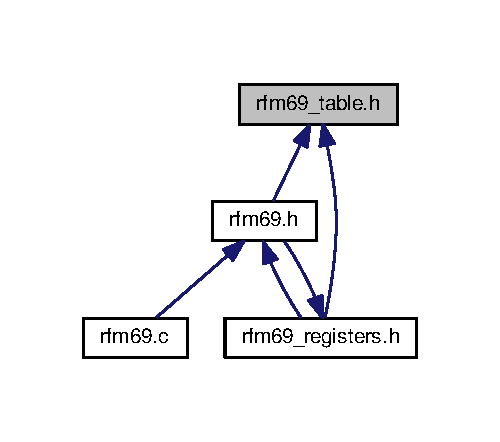
\includegraphics[width=240pt]{rfm69__table_8h__dep__incl}
\end{center}
\end{figure}
\subsection*{Макросы}
\begin{DoxyCompactItemize}
\item 
\#define \hyperlink{rfm69__table_8h_ab1c78669a770ddfb58e99c063225f32f}{P\+A\+R\+A\+M\+P}~0x00
\item 
\#define \hyperlink{rfm69__table_8h_ace6927011fd37b5dc2907de601ae5a8f}{C\+U\+T\+\_\+\+O\+F\+F\+\_\+\+F\+R\+E\+Q\+\_\+\+M100}~\hyperlink{rfm69_8h_a53532033984f6c3768b7f0198559bf2e}{C\+U\+T\+\_\+\+O\+F\+F\+\_\+\+F\+R\+E\+Q}$\ast$100
\item 
\#define \hyperlink{rfm69__table_8h_ab71f13b081475714ab5771e81883f06a}{R\+X\+\_\+\+B\+W\+\_\+\+M10}~\hyperlink{rfm69_8h_a4a4e7a01439b700bd3a6becd6dd122e0}{R\+X\+\_\+\+B\+W}$\ast$10
\item 
\#define \hyperlink{rfm69__table_8h_ade419dfc07a685580dd336aa324f17ad}{R\+X\+B\+W}~0x17
\item 
\#define \hyperlink{rfm69__table_8h_a926e5b6dd5c82bd98949b9927ce907a4}{C\+U\+T\+\_\+\+O\+F\+F\+\_\+\+F\+R\+E\+Q\+\_\+\+A\+F\+C\+\_\+\+M100}~\hyperlink{rfm69_8h_a852de8dab119942f450faa8722897b5b}{C\+U\+T\+\_\+\+O\+F\+F\+\_\+\+F\+R\+E\+Q\+\_\+\+A\+F\+C}$\ast$100
\item 
\#define \hyperlink{rfm69__table_8h_ac42052e2c49c4c1c478ed1af8fc2bd85}{R\+X\+\_\+\+B\+W\+\_\+\+A\+F\+C\+\_\+\+M10}~\hyperlink{rfm69_8h_aa8796d662eb191d6f49e303b9be80e50}{R\+X\+\_\+\+B\+W\+\_\+\+A\+F\+C}$\ast$10
\item 
\#define \hyperlink{rfm69__table_8h_a0f7037bb17d86e8987b9967bed0d473c}{O\+O\+K\+\_\+\+P\+E\+A\+K\+\_\+\+T\+H\+R\+E\+S\+H\+\_\+\+S\+T\+E\+P\+\_\+\+M10}~O\+O\+K\+\_\+\+P\+E\+A\+K\+\_\+\+T\+H\+R\+E\+S\+H\+\_\+\+S\+T\+E\+P$\ast$10
\item 
\#define \hyperlink{rfm69__table_8h_ae79f8e289893175157565ac4be40c063}{O\+O\+K\+\_\+\+P\+E\+A\+K\+\_\+\+T\+H\+R\+E\+S\+H\+\_\+\+D\+E\+C\+\_\+\+M100}~\hyperlink{rfm69_8h_af123b4ef96eb56f98e73951ab76ce314}{O\+O\+K\+\_\+\+P\+E\+A\+K\+\_\+\+T\+H\+R\+E\+S\+H\+\_\+\+D\+E\+C}$\ast$100
\item 
\#define \hyperlink{rfm69__table_8h_aa2f9059f987d6088a0b77a2af76e3ab2}{I\+N\+T\+E\+R\+P\+A\+C\+K\+E\+T\+R\+X\+D\+E\+L\+A\+Y}~0x00
\end{DoxyCompactItemize}


\subsection{Макросы}
\hypertarget{rfm69__table_8h_a926e5b6dd5c82bd98949b9927ce907a4}{\index{rfm69\+\_\+table.\+h@{rfm69\+\_\+table.\+h}!C\+U\+T\+\_\+\+O\+F\+F\+\_\+\+F\+R\+E\+Q\+\_\+\+A\+F\+C\+\_\+\+M100@{C\+U\+T\+\_\+\+O\+F\+F\+\_\+\+F\+R\+E\+Q\+\_\+\+A\+F\+C\+\_\+\+M100}}
\index{C\+U\+T\+\_\+\+O\+F\+F\+\_\+\+F\+R\+E\+Q\+\_\+\+A\+F\+C\+\_\+\+M100@{C\+U\+T\+\_\+\+O\+F\+F\+\_\+\+F\+R\+E\+Q\+\_\+\+A\+F\+C\+\_\+\+M100}!rfm69\+\_\+table.\+h@{rfm69\+\_\+table.\+h}}
\subsubsection[{C\+U\+T\+\_\+\+O\+F\+F\+\_\+\+F\+R\+E\+Q\+\_\+\+A\+F\+C\+\_\+\+M100}]{\setlength{\rightskip}{0pt plus 5cm}\#define C\+U\+T\+\_\+\+O\+F\+F\+\_\+\+F\+R\+E\+Q\+\_\+\+A\+F\+C\+\_\+\+M100~{\bf C\+U\+T\+\_\+\+O\+F\+F\+\_\+\+F\+R\+E\+Q\+\_\+\+A\+F\+C}$\ast$100}}\label{rfm69__table_8h_a926e5b6dd5c82bd98949b9927ce907a4}
\hypertarget{rfm69__table_8h_ace6927011fd37b5dc2907de601ae5a8f}{\index{rfm69\+\_\+table.\+h@{rfm69\+\_\+table.\+h}!C\+U\+T\+\_\+\+O\+F\+F\+\_\+\+F\+R\+E\+Q\+\_\+\+M100@{C\+U\+T\+\_\+\+O\+F\+F\+\_\+\+F\+R\+E\+Q\+\_\+\+M100}}
\index{C\+U\+T\+\_\+\+O\+F\+F\+\_\+\+F\+R\+E\+Q\+\_\+\+M100@{C\+U\+T\+\_\+\+O\+F\+F\+\_\+\+F\+R\+E\+Q\+\_\+\+M100}!rfm69\+\_\+table.\+h@{rfm69\+\_\+table.\+h}}
\subsubsection[{C\+U\+T\+\_\+\+O\+F\+F\+\_\+\+F\+R\+E\+Q\+\_\+\+M100}]{\setlength{\rightskip}{0pt plus 5cm}\#define C\+U\+T\+\_\+\+O\+F\+F\+\_\+\+F\+R\+E\+Q\+\_\+\+M100~{\bf C\+U\+T\+\_\+\+O\+F\+F\+\_\+\+F\+R\+E\+Q}$\ast$100}}\label{rfm69__table_8h_ace6927011fd37b5dc2907de601ae5a8f}
\hypertarget{rfm69__table_8h_aa2f9059f987d6088a0b77a2af76e3ab2}{\index{rfm69\+\_\+table.\+h@{rfm69\+\_\+table.\+h}!I\+N\+T\+E\+R\+P\+A\+C\+K\+E\+T\+R\+X\+D\+E\+L\+A\+Y@{I\+N\+T\+E\+R\+P\+A\+C\+K\+E\+T\+R\+X\+D\+E\+L\+A\+Y}}
\index{I\+N\+T\+E\+R\+P\+A\+C\+K\+E\+T\+R\+X\+D\+E\+L\+A\+Y@{I\+N\+T\+E\+R\+P\+A\+C\+K\+E\+T\+R\+X\+D\+E\+L\+A\+Y}!rfm69\+\_\+table.\+h@{rfm69\+\_\+table.\+h}}
\subsubsection[{I\+N\+T\+E\+R\+P\+A\+C\+K\+E\+T\+R\+X\+D\+E\+L\+A\+Y}]{\setlength{\rightskip}{0pt plus 5cm}\#define I\+N\+T\+E\+R\+P\+A\+C\+K\+E\+T\+R\+X\+D\+E\+L\+A\+Y~0x00}}\label{rfm69__table_8h_aa2f9059f987d6088a0b77a2af76e3ab2}
\hypertarget{rfm69__table_8h_ae79f8e289893175157565ac4be40c063}{\index{rfm69\+\_\+table.\+h@{rfm69\+\_\+table.\+h}!O\+O\+K\+\_\+\+P\+E\+A\+K\+\_\+\+T\+H\+R\+E\+S\+H\+\_\+\+D\+E\+C\+\_\+\+M100@{O\+O\+K\+\_\+\+P\+E\+A\+K\+\_\+\+T\+H\+R\+E\+S\+H\+\_\+\+D\+E\+C\+\_\+\+M100}}
\index{O\+O\+K\+\_\+\+P\+E\+A\+K\+\_\+\+T\+H\+R\+E\+S\+H\+\_\+\+D\+E\+C\+\_\+\+M100@{O\+O\+K\+\_\+\+P\+E\+A\+K\+\_\+\+T\+H\+R\+E\+S\+H\+\_\+\+D\+E\+C\+\_\+\+M100}!rfm69\+\_\+table.\+h@{rfm69\+\_\+table.\+h}}
\subsubsection[{O\+O\+K\+\_\+\+P\+E\+A\+K\+\_\+\+T\+H\+R\+E\+S\+H\+\_\+\+D\+E\+C\+\_\+\+M100}]{\setlength{\rightskip}{0pt plus 5cm}\#define O\+O\+K\+\_\+\+P\+E\+A\+K\+\_\+\+T\+H\+R\+E\+S\+H\+\_\+\+D\+E\+C\+\_\+\+M100~{\bf O\+O\+K\+\_\+\+P\+E\+A\+K\+\_\+\+T\+H\+R\+E\+S\+H\+\_\+\+D\+E\+C}$\ast$100}}\label{rfm69__table_8h_ae79f8e289893175157565ac4be40c063}
\hypertarget{rfm69__table_8h_a0f7037bb17d86e8987b9967bed0d473c}{\index{rfm69\+\_\+table.\+h@{rfm69\+\_\+table.\+h}!O\+O\+K\+\_\+\+P\+E\+A\+K\+\_\+\+T\+H\+R\+E\+S\+H\+\_\+\+S\+T\+E\+P\+\_\+\+M10@{O\+O\+K\+\_\+\+P\+E\+A\+K\+\_\+\+T\+H\+R\+E\+S\+H\+\_\+\+S\+T\+E\+P\+\_\+\+M10}}
\index{O\+O\+K\+\_\+\+P\+E\+A\+K\+\_\+\+T\+H\+R\+E\+S\+H\+\_\+\+S\+T\+E\+P\+\_\+\+M10@{O\+O\+K\+\_\+\+P\+E\+A\+K\+\_\+\+T\+H\+R\+E\+S\+H\+\_\+\+S\+T\+E\+P\+\_\+\+M10}!rfm69\+\_\+table.\+h@{rfm69\+\_\+table.\+h}}
\subsubsection[{O\+O\+K\+\_\+\+P\+E\+A\+K\+\_\+\+T\+H\+R\+E\+S\+H\+\_\+\+S\+T\+E\+P\+\_\+\+M10}]{\setlength{\rightskip}{0pt plus 5cm}\#define O\+O\+K\+\_\+\+P\+E\+A\+K\+\_\+\+T\+H\+R\+E\+S\+H\+\_\+\+S\+T\+E\+P\+\_\+\+M10~O\+O\+K\+\_\+\+P\+E\+A\+K\+\_\+\+T\+H\+R\+E\+S\+H\+\_\+\+S\+T\+E\+P$\ast$10}}\label{rfm69__table_8h_a0f7037bb17d86e8987b9967bed0d473c}
\hypertarget{rfm69__table_8h_ab1c78669a770ddfb58e99c063225f32f}{\index{rfm69\+\_\+table.\+h@{rfm69\+\_\+table.\+h}!P\+A\+R\+A\+M\+P@{P\+A\+R\+A\+M\+P}}
\index{P\+A\+R\+A\+M\+P@{P\+A\+R\+A\+M\+P}!rfm69\+\_\+table.\+h@{rfm69\+\_\+table.\+h}}
\subsubsection[{P\+A\+R\+A\+M\+P}]{\setlength{\rightskip}{0pt plus 5cm}\#define P\+A\+R\+A\+M\+P~0x00}}\label{rfm69__table_8h_ab1c78669a770ddfb58e99c063225f32f}
\hypertarget{rfm69__table_8h_ac42052e2c49c4c1c478ed1af8fc2bd85}{\index{rfm69\+\_\+table.\+h@{rfm69\+\_\+table.\+h}!R\+X\+\_\+\+B\+W\+\_\+\+A\+F\+C\+\_\+\+M10@{R\+X\+\_\+\+B\+W\+\_\+\+A\+F\+C\+\_\+\+M10}}
\index{R\+X\+\_\+\+B\+W\+\_\+\+A\+F\+C\+\_\+\+M10@{R\+X\+\_\+\+B\+W\+\_\+\+A\+F\+C\+\_\+\+M10}!rfm69\+\_\+table.\+h@{rfm69\+\_\+table.\+h}}
\subsubsection[{R\+X\+\_\+\+B\+W\+\_\+\+A\+F\+C\+\_\+\+M10}]{\setlength{\rightskip}{0pt plus 5cm}\#define R\+X\+\_\+\+B\+W\+\_\+\+A\+F\+C\+\_\+\+M10~{\bf R\+X\+\_\+\+B\+W\+\_\+\+A\+F\+C}$\ast$10}}\label{rfm69__table_8h_ac42052e2c49c4c1c478ed1af8fc2bd85}
\hypertarget{rfm69__table_8h_ab71f13b081475714ab5771e81883f06a}{\index{rfm69\+\_\+table.\+h@{rfm69\+\_\+table.\+h}!R\+X\+\_\+\+B\+W\+\_\+\+M10@{R\+X\+\_\+\+B\+W\+\_\+\+M10}}
\index{R\+X\+\_\+\+B\+W\+\_\+\+M10@{R\+X\+\_\+\+B\+W\+\_\+\+M10}!rfm69\+\_\+table.\+h@{rfm69\+\_\+table.\+h}}
\subsubsection[{R\+X\+\_\+\+B\+W\+\_\+\+M10}]{\setlength{\rightskip}{0pt plus 5cm}\#define R\+X\+\_\+\+B\+W\+\_\+\+M10~{\bf R\+X\+\_\+\+B\+W}$\ast$10}}\label{rfm69__table_8h_ab71f13b081475714ab5771e81883f06a}
\hypertarget{rfm69__table_8h_ade419dfc07a685580dd336aa324f17ad}{\index{rfm69\+\_\+table.\+h@{rfm69\+\_\+table.\+h}!R\+X\+B\+W@{R\+X\+B\+W}}
\index{R\+X\+B\+W@{R\+X\+B\+W}!rfm69\+\_\+table.\+h@{rfm69\+\_\+table.\+h}}
\subsubsection[{R\+X\+B\+W}]{\setlength{\rightskip}{0pt plus 5cm}\#define R\+X\+B\+W~0x17}}\label{rfm69__table_8h_ade419dfc07a685580dd336aa324f17ad}

%--- End generated contents ---

% Index
\newpage
\phantomsection
\addcontentsline{toc}{chapter}{Алфавитный указатель}
\printindex

\end{document}
